\documentclass[twoside]{book}

% Packages required by doxygen
\usepackage{calc}
\usepackage{doxygen}
\usepackage{graphicx}
\usepackage[utf8]{inputenc}
\usepackage{makeidx}
\usepackage{multicol}
\usepackage{multirow}
\usepackage{textcomp}
\usepackage[table]{xcolor}

% Font selection
\usepackage[T1]{fontenc}
\usepackage{mathptmx}
\usepackage[scaled=.90]{helvet}
\usepackage{courier}
\usepackage{amssymb}
\usepackage{sectsty}
\renewcommand{\familydefault}{\sfdefault}
\allsectionsfont{%
  \fontseries{bc}\selectfont%
  \color{darkgray}%
}
\renewcommand{\DoxyLabelFont}{%
  \fontseries{bc}\selectfont%
  \color{darkgray}%
}

% Page & text layout
\usepackage{geometry}
\geometry{%
  a4paper,%
  top=2.5cm,%
  bottom=2.5cm,%
  left=2.5cm,%
  right=2.5cm%
}
\tolerance=750
\hfuzz=15pt
\hbadness=750
\setlength{\emergencystretch}{15pt}
\setlength{\parindent}{0cm}
\setlength{\parskip}{0.2cm}
\makeatletter
\renewcommand{\paragraph}{%
  \@startsection{paragraph}{4}{0ex}{-1.0ex}{1.0ex}{%
    \normalfont\normalsize\bfseries\SS@parafont%
  }%
}
\renewcommand{\subparagraph}{%
  \@startsection{subparagraph}{5}{0ex}{-1.0ex}{1.0ex}{%
    \normalfont\normalsize\bfseries\SS@subparafont%
  }%
}
\makeatother

% Headers & footers
\usepackage{fancyhdr}
\pagestyle{fancyplain}
\fancyhead[LE]{\fancyplain{}{\bfseries\thepage}}
\fancyhead[CE]{\fancyplain{}{}}
\fancyhead[RE]{\fancyplain{}{\bfseries\leftmark}}
\fancyhead[LO]{\fancyplain{}{\bfseries\rightmark}}
\fancyhead[CO]{\fancyplain{}{}}
\fancyhead[RO]{\fancyplain{}{\bfseries\thepage}}
\fancyfoot[LE]{\fancyplain{}{}}
\fancyfoot[CE]{\fancyplain{}{}}
\fancyfoot[RE]{\fancyplain{}{\bfseries\scriptsize Generated on Thu Nov 20 2014 17\-:49\-:29 for F\-C\-A\-L to C++ Translator by Doxygen }}
\fancyfoot[LO]{\fancyplain{}{\bfseries\scriptsize Generated on Thu Nov 20 2014 17\-:49\-:29 for F\-C\-A\-L to C++ Translator by Doxygen }}
\fancyfoot[CO]{\fancyplain{}{}}
\fancyfoot[RO]{\fancyplain{}{}}
\renewcommand{\footrulewidth}{0.4pt}
\renewcommand{\chaptermark}[1]{%
  \markboth{#1}{}%
}
\renewcommand{\sectionmark}[1]{%
  \markright{\thesection\ #1}%
}

% Indices & bibliography
\usepackage{natbib}
\usepackage[titles]{tocloft}
\setcounter{tocdepth}{3}
\setcounter{secnumdepth}{5}
\makeindex

% Hyperlinks (required, but should be loaded last)
\usepackage{ifpdf}
\ifpdf
  \usepackage[pdftex,pagebackref=true]{hyperref}
\else
  \usepackage[ps2pdf,pagebackref=true]{hyperref}
\fi
\hypersetup{%
  colorlinks=true,%
  linkcolor=blue,%
  citecolor=blue,%
  unicode%
}

% Custom commands
\newcommand{\clearemptydoublepage}{%
  \newpage{\pagestyle{empty}\cleardoublepage}%
}


%===== C O N T E N T S =====

\begin{document}

% Titlepage & ToC
\hypersetup{pageanchor=false}
\pagenumbering{roman}
\begin{titlepage}
\vspace*{7cm}
\begin{center}%
{\Large F\-C\-A\-L to C++ Translator }\\
\vspace*{1cm}
{\large Generated by Doxygen 1.8.6}\\
\vspace*{0.5cm}
{\small Thu Nov 20 2014 17:49:29}\\
\end{center}
\end{titlepage}
\clearemptydoublepage
\tableofcontents
\clearemptydoublepage
\pagenumbering{arabic}
\hypersetup{pageanchor=true}

%--- Begin generated contents ---
\chapter{My Personal Index Page}
\label{index}\hypertarget{index}{}\hypertarget{index_intro_sec}{}\section{Introduction}\label{index_intro_sec}
This is the introduction.\hypertarget{index_install_sec}{}\section{Installation}\label{index_install_sec}
This is how you make or install my software\hypertarget{index_step1}{}\subsection{Step 1\-: Opening the box}\label{index_step1}
Here is some more details. 
\chapter{Hierarchical Index}
\section{Class Hierarchy}
This inheritance list is sorted roughly, but not completely, alphabetically\-:\begin{DoxyCompactList}
\item \contentsline{section}{Ext\-Token}{\pageref{classExtToken}}{}
\begin{DoxyCompactList}
\item \contentsline{section}{Char\-Const\-Token}{\pageref{classCharConstToken}}{}
\item \contentsline{section}{Dash\-Token}{\pageref{classDashToken}}{}
\item \contentsline{section}{End\-Of\-File\-Token}{\pageref{classEndOfFileToken}}{}
\item \contentsline{section}{False\-Kwd\-Token}{\pageref{classFalseKwdToken}}{}
\item \contentsline{section}{Float\-Const\-Token}{\pageref{classFloatConstToken}}{}
\item \contentsline{section}{Forward\-Slash\-Token}{\pageref{classForwardSlashToken}}{}
\item \contentsline{section}{If\-Token}{\pageref{classIfToken}}{}
\item \contentsline{section}{Int\-Const\-Token}{\pageref{classIntConstToken}}{}
\item \contentsline{section}{Left\-Paren\-Token}{\pageref{classLeftParenToken}}{}
\item \contentsline{section}{Let\-Token}{\pageref{classLetToken}}{}
\item \contentsline{section}{Not\-Op\-Token}{\pageref{classNotOpToken}}{}
\item \contentsline{section}{Plus\-Sign\-Token}{\pageref{classPlusSignToken}}{}
\item \contentsline{section}{Relational\-Op\-Token}{\pageref{classRelationalOpToken}}{}
\item \contentsline{section}{Star\-Token}{\pageref{classStarToken}}{}
\item \contentsline{section}{String\-Const\-Token}{\pageref{classStringConstToken}}{}
\item \contentsline{section}{True\-Kwd\-Token}{\pageref{classTrueKwdToken}}{}
\item \contentsline{section}{Variable\-Name\-Token}{\pageref{classVariableNameToken}}{}
\end{DoxyCompactList}
\item \contentsline{section}{Node}{\pageref{classNode}}{}
\begin{DoxyCompactList}
\item \contentsline{section}{Expr}{\pageref{classExpr}}{}
\begin{DoxyCompactList}
\item \contentsline{section}{Any\-Const}{\pageref{classAnyConst}}{}
\item \contentsline{section}{Bin\-Op\-Expr}{\pageref{classBinOpExpr}}{}
\item \contentsline{section}{Function\-Call}{\pageref{classFunctionCall}}{}
\item \contentsline{section}{If\-Expr}{\pageref{classIfExpr}}{}
\item \contentsline{section}{Let\-Expr}{\pageref{classLetExpr}}{}
\item \contentsline{section}{Matrix\-Ref\-Expr}{\pageref{classMatrixRefExpr}}{}
\item \contentsline{section}{Not\-Expr}{\pageref{classNotExpr}}{}
\item \contentsline{section}{Parens\-Expr}{\pageref{classParensExpr}}{}
\item \contentsline{section}{Var\-Name}{\pageref{classVarName}}{}
\end{DoxyCompactList}
\item \contentsline{section}{Root}{\pageref{classRoot}}{}
\item \contentsline{section}{Stmt}{\pageref{classStmt}}{}
\begin{DoxyCompactList}
\item \contentsline{section}{For\-Stmt}{\pageref{classForStmt}}{}
\item \contentsline{section}{If\-Else\-Stmt}{\pageref{classIfElseStmt}}{}
\item \contentsline{section}{If\-Stmt}{\pageref{classIfStmt}}{}
\item \contentsline{section}{Matrix\-Adv\-Decl}{\pageref{classMatrixAdvDecl}}{}
\item \contentsline{section}{Matrix\-Assign\-Stmt}{\pageref{classMatrixAssignStmt}}{}
\item \contentsline{section}{Matrix\-Decl}{\pageref{classMatrixDecl}}{}
\item \contentsline{section}{Print\-Stmt}{\pageref{classPrintStmt}}{}
\item \contentsline{section}{Standard\-Assign\-Stmt}{\pageref{classStandardAssignStmt}}{}
\item \contentsline{section}{Standard\-Decl}{\pageref{classStandardDecl}}{}
\item \contentsline{section}{Stmt\-Block}{\pageref{classStmtBlock}}{}
\item \contentsline{section}{While\-Stmt}{\pageref{classWhileStmt}}{}
\end{DoxyCompactList}
\item \contentsline{section}{Stmts}{\pageref{classStmts}}{}
\begin{DoxyCompactList}
\item \contentsline{section}{Empty\-Stmts}{\pageref{classEmptyStmts}}{}
\item \contentsline{section}{Stmt\-Stmts}{\pageref{classStmtStmts}}{}
\end{DoxyCompactList}
\end{DoxyCompactList}
\item \contentsline{section}{Parser}{\pageref{classParser}}{}
\item \contentsline{section}{Parse\-Result}{\pageref{classParseResult}}{}
\item \contentsline{section}{Scanner}{\pageref{classScanner}}{}
\item Test\-Suite\begin{DoxyCompactList}
\item \contentsline{section}{Ast\-Test\-Suite}{\pageref{classAstTestSuite}}{}
\item \contentsline{section}{Parser\-Test\-Suite}{\pageref{classParserTestSuite}}{}
\item \contentsline{section}{Regex\-Test\-Suite}{\pageref{classRegexTestSuite}}{}
\item \contentsline{section}{Scanner\-Test\-Suite}{\pageref{classScannerTestSuite}}{}
\end{DoxyCompactList}
\item \contentsline{section}{Token}{\pageref{classToken}}{}
\end{DoxyCompactList}

\chapter{Class Index}
\section{Class List}
Here are the classes, structs, unions and interfaces with brief descriptions\-:\begin{DoxyCompactList}
\item\contentsline{section}{\hyperlink{classAnyConst}{Any\-Const} \\*Represents a constant -\/ of any type (string, int, float, etc...). \par
 }{\pageref{classAnyConst}}{}
\item\contentsline{section}{\hyperlink{classAstTestSuite}{Ast\-Test\-Suite} }{\pageref{classAstTestSuite}}{}
\item\contentsline{section}{\hyperlink{classBinOpExpr}{Bin\-Op\-Expr} \\*Represents two expressions separated by an operation. \par
 }{\pageref{classBinOpExpr}}{}
\item\contentsline{section}{\hyperlink{classCharConstToken}{Char\-Const\-Token} }{\pageref{classCharConstToken}}{}
\item\contentsline{section}{\hyperlink{classDashToken}{Dash\-Token} }{\pageref{classDashToken}}{}
\item\contentsline{section}{\hyperlink{classEmptyStmts}{Empty\-Stmts} \\*Represents emptiness }{\pageref{classEmptyStmts}}{}
\item\contentsline{section}{\hyperlink{classEndOfFileToken}{End\-Of\-File\-Token} }{\pageref{classEndOfFileToken}}{}
\item\contentsline{section}{\hyperlink{classExpr}{Expr} \\*Parent for all expression instances to be parsed \par
 }{\pageref{classExpr}}{}
\item\contentsline{section}{\hyperlink{classExtToken}{Ext\-Token} }{\pageref{classExtToken}}{}
\item\contentsline{section}{\hyperlink{classFalseKwdToken}{False\-Kwd\-Token} }{\pageref{classFalseKwdToken}}{}
\item\contentsline{section}{\hyperlink{classFloatConstToken}{Float\-Const\-Token} }{\pageref{classFloatConstToken}}{}
\item\contentsline{section}{\hyperlink{classForStmt}{For\-Stmt} \\*Represents a for-\/loop statement. \par
 }{\pageref{classForStmt}}{}
\item\contentsline{section}{\hyperlink{classForwardSlashToken}{Forward\-Slash\-Token} }{\pageref{classForwardSlashToken}}{}
\item\contentsline{section}{\hyperlink{classFunctionCall}{Function\-Call} \\*Represents a function call. \par
 }{\pageref{classFunctionCall}}{}
\item\contentsline{section}{\hyperlink{classIfElseStmt}{If\-Else\-Stmt} \\*Represents an if-\/else statement. \par
 }{\pageref{classIfElseStmt}}{}
\item\contentsline{section}{\hyperlink{classIfExpr}{If\-Expr} \\*Represents if-\/then-\/else expression \par
 }{\pageref{classIfExpr}}{}
\item\contentsline{section}{\hyperlink{classIfStmt}{If\-Stmt} \\*Represents an if statement. \par
 }{\pageref{classIfStmt}}{}
\item\contentsline{section}{\hyperlink{classIfToken}{If\-Token} }{\pageref{classIfToken}}{}
\item\contentsline{section}{\hyperlink{classIntConstToken}{Int\-Const\-Token} }{\pageref{classIntConstToken}}{}
\item\contentsline{section}{\hyperlink{classLeftParenToken}{Left\-Paren\-Token} }{\pageref{classLeftParenToken}}{}
\item\contentsline{section}{\hyperlink{classLetExpr}{Let\-Expr} \\*Represents a let expression. \par
 }{\pageref{classLetExpr}}{}
\item\contentsline{section}{\hyperlink{classLetToken}{Let\-Token} }{\pageref{classLetToken}}{}
\item\contentsline{section}{\hyperlink{classMatrixAdvDecl}{Matrix\-Adv\-Decl} \\*Represents a declaration of a matrix with initial values. \par
 }{\pageref{classMatrixAdvDecl}}{}
\item\contentsline{section}{\hyperlink{classMatrixAssignStmt}{Matrix\-Assign\-Stmt} \\*Represents a matrix assignment. \par
 }{\pageref{classMatrixAssignStmt}}{}
\item\contentsline{section}{\hyperlink{classMatrixDecl}{Matrix\-Decl} \\*Represents a standard declaration of a matrix. \par
 }{\pageref{classMatrixDecl}}{}
\item\contentsline{section}{\hyperlink{classMatrixRefExpr}{Matrix\-Ref\-Expr} \\*Represents accessing a matrix. \par
 }{\pageref{classMatrixRefExpr}}{}
\item\contentsline{section}{\hyperlink{classNode}{Node} \\*Abstract parent or grandparent for all classes in the Abstract Syntax Tree (A\-S\-T) }{\pageref{classNode}}{}
\item\contentsline{section}{\hyperlink{classNotExpr}{Not\-Expr} \\*Represents negation of a boolean \par
 }{\pageref{classNotExpr}}{}
\item\contentsline{section}{\hyperlink{classNotOpToken}{Not\-Op\-Token} }{\pageref{classNotOpToken}}{}
\item\contentsline{section}{\hyperlink{classParensExpr}{Parens\-Expr} \\*Represents an expression surrounded by parenthesis. \par
 }{\pageref{classParensExpr}}{}
\item\contentsline{section}{\hyperlink{classParser}{Parser} \\*Organizes F\-C\-A\-L text into an tree }{\pageref{classParser}}{}
\item\contentsline{section}{\hyperlink{classParseResult}{Parse\-Result} }{\pageref{classParseResult}}{}
\item\contentsline{section}{\hyperlink{classParserTestSuite}{Parser\-Test\-Suite} }{\pageref{classParserTestSuite}}{}
\item\contentsline{section}{\hyperlink{classPlusSignToken}{Plus\-Sign\-Token} }{\pageref{classPlusSignToken}}{}
\item\contentsline{section}{\hyperlink{classPrintStmt}{Print\-Stmt} \\*Represents a print statement. \par
 }{\pageref{classPrintStmt}}{}
\item\contentsline{section}{\hyperlink{classRegexTestSuite}{Regex\-Test\-Suite} }{\pageref{classRegexTestSuite}}{}
\item\contentsline{section}{\hyperlink{classRelationalOpToken}{Relational\-Op\-Token} }{\pageref{classRelationalOpToken}}{}
\item\contentsline{section}{\hyperlink{classRoot}{Root} \\*Handles initial function declaration }{\pageref{classRoot}}{}
\item\contentsline{section}{\hyperlink{classScanner}{Scanner} }{\pageref{classScanner}}{}
\item\contentsline{section}{\hyperlink{classScannerTestSuite}{Scanner\-Test\-Suite} }{\pageref{classScannerTestSuite}}{}
\item\contentsline{section}{\hyperlink{classStandardAssignStmt}{Standard\-Assign\-Stmt} \\*Represents a standard variable assignment. \par
 }{\pageref{classStandardAssignStmt}}{}
\item\contentsline{section}{\hyperlink{classStandardDecl}{Standard\-Decl} \\*Represents a declaration of a variable \par
 }{\pageref{classStandardDecl}}{}
\item\contentsline{section}{\hyperlink{classStarToken}{Star\-Token} }{\pageref{classStarToken}}{}
\item\contentsline{section}{\hyperlink{classStmt}{Stmt} \\*Parent for all statment instances to be parsed \par
 }{\pageref{classStmt}}{}
\item\contentsline{section}{\hyperlink{classStmtBlock}{Stmt\-Block} \\*Represents a stmt which contains a block of stmts. \par
 }{\pageref{classStmtBlock}}{}
\item\contentsline{section}{\hyperlink{classStmts}{Stmts} \\*Parent for all statements to be parsed }{\pageref{classStmts}}{}
\item\contentsline{section}{\hyperlink{classStmtStmts}{Stmt\-Stmts} \\*This provides a gateway to stmt objects. Without this, there would only be \par
 \hyperlink{classStmts}{Stmts} and no \hyperlink{classStmt}{Stmt} would be able to be parsed }{\pageref{classStmtStmts}}{}
\item\contentsline{section}{\hyperlink{classStringConstToken}{String\-Const\-Token} }{\pageref{classStringConstToken}}{}
\item\contentsline{section}{\hyperlink{classToken}{Token} }{\pageref{classToken}}{}
\item\contentsline{section}{\hyperlink{classTrueKwdToken}{True\-Kwd\-Token} }{\pageref{classTrueKwdToken}}{}
\item\contentsline{section}{\hyperlink{classVariableNameToken}{Variable\-Name\-Token} }{\pageref{classVariableNameToken}}{}
\item\contentsline{section}{\hyperlink{classVarName}{Var\-Name} \\*Represents a variable name. \par
 }{\pageref{classVarName}}{}
\item\contentsline{section}{\hyperlink{classWhileStmt}{While\-Stmt} \\*Represents a while-\/loop statement. \par
 }{\pageref{classWhileStmt}}{}
\end{DoxyCompactList}

\chapter{File Index}
\section{File List}
Here is a list of all files with brief descriptions\-:\begin{DoxyCompactList}
\item\contentsline{section}{\hyperlink{AST_8cpp}{A\-S\-T.\-cpp} }{\pageref{AST_8cpp}}{}
\item\contentsline{section}{\hyperlink{AST_8h}{A\-S\-T.\-h} }{\pageref{AST_8h}}{}
\item\contentsline{section}{\hyperlink{ast__tests_8cpp}{ast\-\_\-tests.\-cpp} }{\pageref{ast__tests_8cpp}}{}
\item\contentsline{section}{\hyperlink{ast__tests_8h}{ast\-\_\-tests.\-h} }{\pageref{ast__tests_8h}}{}
\item\contentsline{section}{\hyperlink{extToken_8cpp}{ext\-Token.\-cpp} }{\pageref{extToken_8cpp}}{}
\item\contentsline{section}{\hyperlink{extToken_8h}{ext\-Token.\-h} }{\pageref{extToken_8h}}{}
\item\contentsline{section}{\hyperlink{mainpage_8h}{mainpage.\-h} }{\pageref{mainpage_8h}}{}
\item\contentsline{section}{\hyperlink{parser_8cpp}{parser.\-cpp} }{\pageref{parser_8cpp}}{}
\item\contentsline{section}{\hyperlink{parser_8h}{parser.\-h} }{\pageref{parser_8h}}{}
\item\contentsline{section}{\hyperlink{parser__tests_8cpp}{parser\-\_\-tests.\-cpp} }{\pageref{parser__tests_8cpp}}{}
\item\contentsline{section}{\hyperlink{parser__tests_8h}{parser\-\_\-tests.\-h} }{\pageref{parser__tests_8h}}{}
\item\contentsline{section}{\hyperlink{parseResult_8cpp}{parse\-Result.\-cpp} }{\pageref{parseResult_8cpp}}{}
\item\contentsline{section}{\hyperlink{parseResult_8h}{parse\-Result.\-h} }{\pageref{parseResult_8h}}{}
\item\contentsline{section}{\hyperlink{readInput_8cpp}{read\-Input.\-cpp} }{\pageref{readInput_8cpp}}{}
\item\contentsline{section}{\hyperlink{readInput_8h}{read\-Input.\-h} }{\pageref{readInput_8h}}{}
\item\contentsline{section}{\hyperlink{regex_8cpp}{regex.\-cpp} }{\pageref{regex_8cpp}}{}
\item\contentsline{section}{\hyperlink{regex_8h}{regex.\-h} }{\pageref{regex_8h}}{}
\item\contentsline{section}{\hyperlink{regex__tests_8cpp}{regex\-\_\-tests.\-cpp} }{\pageref{regex__tests_8cpp}}{}
\item\contentsline{section}{\hyperlink{regex__tests_8h}{regex\-\_\-tests.\-h} }{\pageref{regex__tests_8h}}{}
\item\contentsline{section}{\hyperlink{scanner_8cpp}{scanner.\-cpp} }{\pageref{scanner_8cpp}}{}
\item\contentsline{section}{\hyperlink{scanner_8h}{scanner.\-h} }{\pageref{scanner_8h}}{}
\item\contentsline{section}{\hyperlink{scanner__tests_8cpp}{scanner\-\_\-tests.\-cpp} }{\pageref{scanner__tests_8cpp}}{}
\item\contentsline{section}{\hyperlink{scanner__tests_8h}{scanner\-\_\-tests.\-h} }{\pageref{scanner__tests_8h}}{}
\end{DoxyCompactList}

\chapter{Class Documentation}
\hypertarget{classAnyConst}{\section{Any\-Const Class Reference}
\label{classAnyConst}\index{Any\-Const@{Any\-Const}}
}


Represents a constant -\/ of any type (string, int, float, etc...). \par
  




{\ttfamily \#include $<$A\-S\-T.\-h$>$}



Inheritance diagram for Any\-Const\-:\nopagebreak
\begin{figure}[H]
\begin{center}
\leavevmode
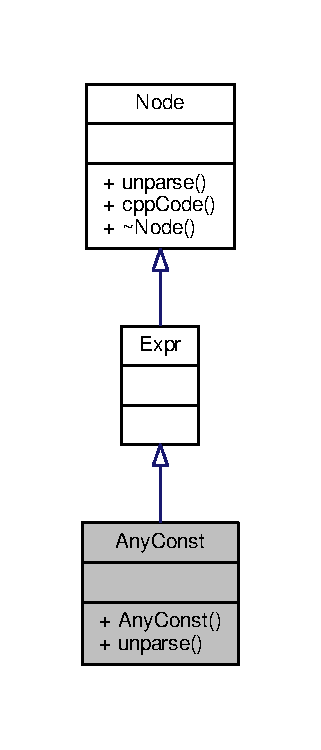
\includegraphics[width=154pt]{classAnyConst__inherit__graph}
\end{center}
\end{figure}


Collaboration diagram for Any\-Const\-:\nopagebreak
\begin{figure}[H]
\begin{center}
\leavevmode
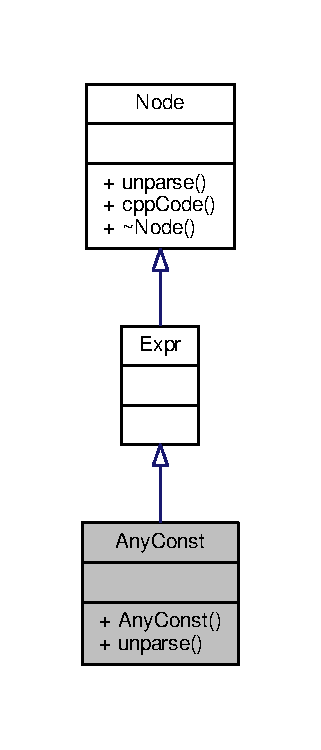
\includegraphics[width=154pt]{classAnyConst__coll__graph}
\end{center}
\end{figure}
\subsection*{Public Member Functions}
\begin{DoxyCompactItemize}
\item 
\hyperlink{classAnyConst_a2ae9135a82a8954e22765ecfec832eea}{Any\-Const} (std\-::string s)
\item 
std\-::string \hyperlink{classAnyConst_a2c4a9d1499b29bde8e72650cae459716}{unparse} ()
\begin{DoxyCompactList}\small\item\em Returns a string representation of the code modeled by this class and all its variables. \end{DoxyCompactList}\end{DoxyCompactItemize}


\subsection{Detailed Description}
Represents a constant -\/ of any type (string, int, float, etc...). \par
 

Model\-: \hyperlink{classExpr}{Expr} \-:\-:= const \par
 Example\-: 100 

\subsection{Constructor \& Destructor Documentation}
\hypertarget{classAnyConst_a2ae9135a82a8954e22765ecfec832eea}{\index{Any\-Const@{Any\-Const}!Any\-Const@{Any\-Const}}
\index{Any\-Const@{Any\-Const}!AnyConst@{Any\-Const}}
\subsubsection[{Any\-Const}]{\setlength{\rightskip}{0pt plus 5cm}Any\-Const\-::\-Any\-Const (
\begin{DoxyParamCaption}
\item[{std\-::string}]{s}
\end{DoxyParamCaption}
)\hspace{0.3cm}{\ttfamily [inline]}}}\label{classAnyConst_a2ae9135a82a8954e22765ecfec832eea}
Public constructor. 
\begin{DoxyParams}{Parameters}
{\em s} & -\/ Value of the constant \\
\hline
\end{DoxyParams}


\subsection{Member Function Documentation}
\hypertarget{classAnyConst_a2c4a9d1499b29bde8e72650cae459716}{\index{Any\-Const@{Any\-Const}!unparse@{unparse}}
\index{unparse@{unparse}!AnyConst@{Any\-Const}}
\subsubsection[{unparse}]{\setlength{\rightskip}{0pt plus 5cm}string Any\-Const\-::unparse (
\begin{DoxyParamCaption}
{}
\end{DoxyParamCaption}
)\hspace{0.3cm}{\ttfamily [virtual]}}}\label{classAnyConst_a2c4a9d1499b29bde8e72650cae459716}


Returns a string representation of the code modeled by this class and all its variables. 

\begin{DoxyReturn}{Returns}
std\-::string. 
\end{DoxyReturn}


Implements \hyperlink{classNode_a60ea533e0900961c05e701db70097136}{Node}.



The documentation for this class was generated from the following files\-:\begin{DoxyCompactItemize}
\item 
\hyperlink{AST_8h}{A\-S\-T.\-h}\item 
\hyperlink{AST_8cpp}{A\-S\-T.\-cpp}\end{DoxyCompactItemize}

\hypertarget{classAstTestSuite}{\section{Ast\-Test\-Suite Class Reference}
\label{classAstTestSuite}\index{Ast\-Test\-Suite@{Ast\-Test\-Suite}}
}


{\ttfamily \#include $<$ast\-\_\-tests.\-h$>$}



Inheritance diagram for Ast\-Test\-Suite\-:\nopagebreak
\begin{figure}[H]
\begin{center}
\leavevmode
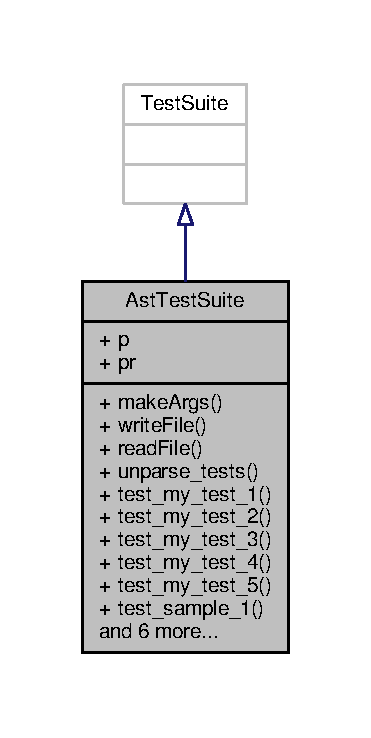
\includegraphics[width=178pt]{classAstTestSuite__inherit__graph}
\end{center}
\end{figure}


Collaboration diagram for Ast\-Test\-Suite\-:\nopagebreak
\begin{figure}[H]
\begin{center}
\leavevmode
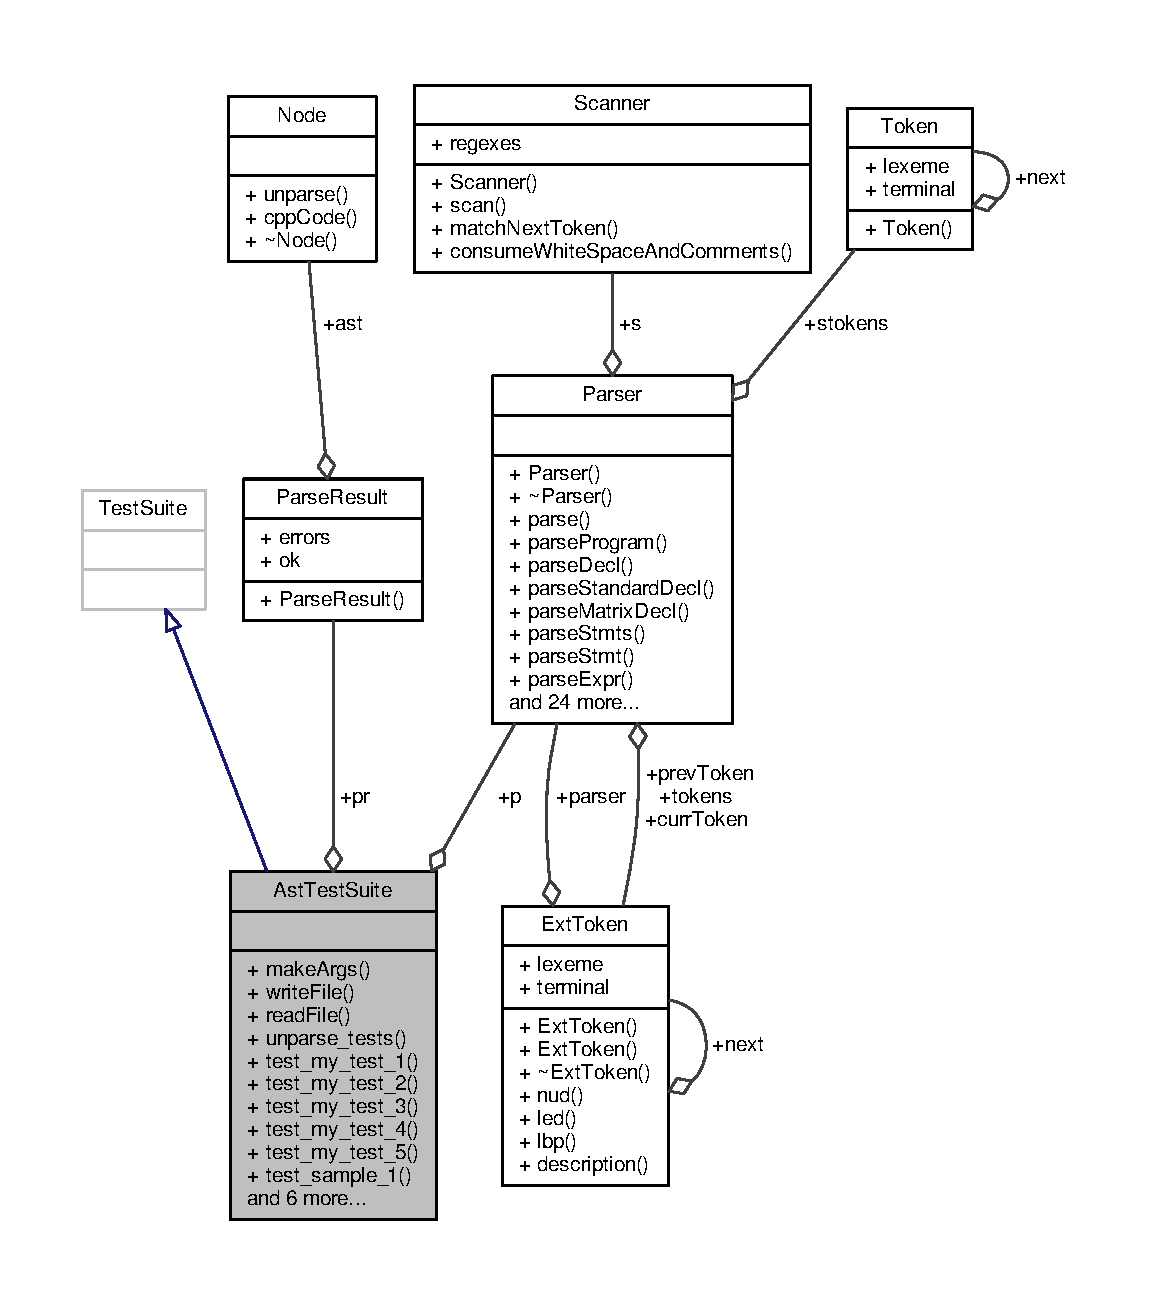
\includegraphics[width=350pt]{classAstTestSuite__coll__graph}
\end{center}
\end{figure}
\subsection*{Public Member Functions}
\begin{DoxyCompactItemize}
\item 
char $\ast$$\ast$ \hyperlink{classAstTestSuite_a2f0462e7a965acda10e09e70432cab40}{make\-Args} (const char $\ast$a0, const char $\ast$a1)
\item 
void \hyperlink{classAstTestSuite_ab935b3c95647b24b5f250b7e3332a313}{write\-File} (const string text, const string filename)
\item 
char $\ast$ \hyperlink{classAstTestSuite_afb1462e2494b011f0e5077a567e0ba3d}{read\-File} (const char $\ast$fn)
\item 
void \hyperlink{classAstTestSuite_a1fb6dcbf82548632381eb89079b456aa}{unparse\-\_\-tests} (string file)
\item 
void \hyperlink{classAstTestSuite_a4cbddb78a689baf1b27a2a49a0865518}{test\-\_\-my\-\_\-test\-\_\-1} ()
\begin{DoxyCompactList}\small\item\em Ensures the root of the function can be parsed. \end{DoxyCompactList}\item 
void \hyperlink{classAstTestSuite_ac7d9c4949e470d827005c1ead8ea124e}{test\-\_\-my\-\_\-test\-\_\-2} ()
\begin{DoxyCompactList}\small\item\em Ensures variables can be declared. \end{DoxyCompactList}\item 
void \hyperlink{classAstTestSuite_a0e62549846c7bf5fec73a3e905489dd3}{test\-\_\-my\-\_\-test\-\_\-3} ()
\begin{DoxyCompactList}\small\item\em Ensures if statements can be parsed and variables can be assigned. \end{DoxyCompactList}\item 
void \hyperlink{classAstTestSuite_aecae8b1ee68f7d09ae460b88db03bc40}{test\-\_\-my\-\_\-test\-\_\-4} ()
\begin{DoxyCompactList}\small\item\em Ensures loops can be parsed and expressions can be printed. \end{DoxyCompactList}\item 
void \hyperlink{classAstTestSuite_a9d44a169841879efae1412b4a59feee5}{test\-\_\-my\-\_\-test\-\_\-5} ()
\begin{DoxyCompactList}\small\item\em Ensures everything can be parsed. \end{DoxyCompactList}\item 
void \hyperlink{classAstTestSuite_ade48304a65cbc7449bd22ec9097b6a8c}{test\-\_\-sample\-\_\-1} (void)
\item 
void \hyperlink{classAstTestSuite_af764267aa9a94610fd5307ae81107312}{test\-\_\-sample\-\_\-2} (void)
\item 
void \hyperlink{classAstTestSuite_a956750fe55d2eb218eb75bd7dc75bc34}{test\-\_\-sample\-\_\-3} (void)
\item 
void \hyperlink{classAstTestSuite_a665836b3d23c82eda3233a3c5d2f0ba4}{test\-\_\-sample\-\_\-4} (void)
\item 
void \hyperlink{classAstTestSuite_a9cceb7f0e5a6714d539f25db38424851}{test\-\_\-sample\-\_\-5} (void)
\item 
void \hyperlink{classAstTestSuite_adbc7de61740aaf9ebf9b7e25f024f318}{test\-\_\-mysample} (void)
\item 
void \hyperlink{classAstTestSuite_ade9231acfe5f8c8f02e00e54749cf99b}{test\-\_\-forest\-\_\-loss} (void)
\end{DoxyCompactItemize}
\subsection*{Public Attributes}
\begin{DoxyCompactItemize}
\item 
\hyperlink{classParser}{Parser} \hyperlink{classAstTestSuite_a148a26ab78abac732d857d7095f6dea5}{p}
\item 
\hyperlink{classParseResult}{Parse\-Result} \hyperlink{classAstTestSuite_ab27964f1743a2889538ca27e644eb1aa}{pr}
\end{DoxyCompactItemize}


\subsection{Member Function Documentation}
\hypertarget{classAstTestSuite_a2f0462e7a965acda10e09e70432cab40}{\index{Ast\-Test\-Suite@{Ast\-Test\-Suite}!make\-Args@{make\-Args}}
\index{make\-Args@{make\-Args}!AstTestSuite@{Ast\-Test\-Suite}}
\subsubsection[{make\-Args}]{\setlength{\rightskip}{0pt plus 5cm}char$\ast$$\ast$ Ast\-Test\-Suite\-::make\-Args (
\begin{DoxyParamCaption}
\item[{const char $\ast$}]{a0, }
\item[{const char $\ast$}]{a1}
\end{DoxyParamCaption}
)\hspace{0.3cm}{\ttfamily [inline]}}}\label{classAstTestSuite_a2f0462e7a965acda10e09e70432cab40}
\hypertarget{classAstTestSuite_afb1462e2494b011f0e5077a567e0ba3d}{\index{Ast\-Test\-Suite@{Ast\-Test\-Suite}!read\-File@{read\-File}}
\index{read\-File@{read\-File}!AstTestSuite@{Ast\-Test\-Suite}}
\subsubsection[{read\-File}]{\setlength{\rightskip}{0pt plus 5cm}char$\ast$ Ast\-Test\-Suite\-::read\-File (
\begin{DoxyParamCaption}
\item[{const char $\ast$}]{fn}
\end{DoxyParamCaption}
)\hspace{0.3cm}{\ttfamily [inline]}}}\label{classAstTestSuite_afb1462e2494b011f0e5077a567e0ba3d}
\hypertarget{classAstTestSuite_ade9231acfe5f8c8f02e00e54749cf99b}{\index{Ast\-Test\-Suite@{Ast\-Test\-Suite}!test\-\_\-forest\-\_\-loss@{test\-\_\-forest\-\_\-loss}}
\index{test\-\_\-forest\-\_\-loss@{test\-\_\-forest\-\_\-loss}!AstTestSuite@{Ast\-Test\-Suite}}
\subsubsection[{test\-\_\-forest\-\_\-loss}]{\setlength{\rightskip}{0pt plus 5cm}void Ast\-Test\-Suite\-::test\-\_\-forest\-\_\-loss (
\begin{DoxyParamCaption}
\item[{void}]{}
\end{DoxyParamCaption}
)\hspace{0.3cm}{\ttfamily [inline]}}}\label{classAstTestSuite_ade9231acfe5f8c8f02e00e54749cf99b}
\hypertarget{classAstTestSuite_a4cbddb78a689baf1b27a2a49a0865518}{\index{Ast\-Test\-Suite@{Ast\-Test\-Suite}!test\-\_\-my\-\_\-test\-\_\-1@{test\-\_\-my\-\_\-test\-\_\-1}}
\index{test\-\_\-my\-\_\-test\-\_\-1@{test\-\_\-my\-\_\-test\-\_\-1}!AstTestSuite@{Ast\-Test\-Suite}}
\subsubsection[{test\-\_\-my\-\_\-test\-\_\-1}]{\setlength{\rightskip}{0pt plus 5cm}void Ast\-Test\-Suite\-::test\-\_\-my\-\_\-test\-\_\-1 (
\begin{DoxyParamCaption}
{}
\end{DoxyParamCaption}
)\hspace{0.3cm}{\ttfamily [inline]}}}\label{classAstTestSuite_a4cbddb78a689baf1b27a2a49a0865518}


Ensures the root of the function can be parsed. 

Tests that \hyperlink{classRoot}{Root} and \hyperlink{classEmptyStmts}{Empty\-Stmts} are correctly integrated into the parser

This was the first test to pass on 11/18/2014 \hypertarget{classAstTestSuite_ac7d9c4949e470d827005c1ead8ea124e}{\index{Ast\-Test\-Suite@{Ast\-Test\-Suite}!test\-\_\-my\-\_\-test\-\_\-2@{test\-\_\-my\-\_\-test\-\_\-2}}
\index{test\-\_\-my\-\_\-test\-\_\-2@{test\-\_\-my\-\_\-test\-\_\-2}!AstTestSuite@{Ast\-Test\-Suite}}
\subsubsection[{test\-\_\-my\-\_\-test\-\_\-2}]{\setlength{\rightskip}{0pt plus 5cm}void Ast\-Test\-Suite\-::test\-\_\-my\-\_\-test\-\_\-2 (
\begin{DoxyParamCaption}
{}
\end{DoxyParamCaption}
)\hspace{0.3cm}{\ttfamily [inline]}}}\label{classAstTestSuite_ac7d9c4949e470d827005c1ead8ea124e}


Ensures variables can be declared. 

Tests that \hyperlink{classStandardDecl}{Standard\-Decl}, \hyperlink{classMatrixDecl}{Matrix\-Decl}, and Matrix\-Advanced\-Decl are all correctly integrated into the parser

This was the second test to pass on 11/18/2014 \hypertarget{classAstTestSuite_a0e62549846c7bf5fec73a3e905489dd3}{\index{Ast\-Test\-Suite@{Ast\-Test\-Suite}!test\-\_\-my\-\_\-test\-\_\-3@{test\-\_\-my\-\_\-test\-\_\-3}}
\index{test\-\_\-my\-\_\-test\-\_\-3@{test\-\_\-my\-\_\-test\-\_\-3}!AstTestSuite@{Ast\-Test\-Suite}}
\subsubsection[{test\-\_\-my\-\_\-test\-\_\-3}]{\setlength{\rightskip}{0pt plus 5cm}void Ast\-Test\-Suite\-::test\-\_\-my\-\_\-test\-\_\-3 (
\begin{DoxyParamCaption}
{}
\end{DoxyParamCaption}
)\hspace{0.3cm}{\ttfamily [inline]}}}\label{classAstTestSuite_a0e62549846c7bf5fec73a3e905489dd3}


Ensures if statements can be parsed and variables can be assigned. 

Tests that \hyperlink{classIfElseStmt}{If\-Else\-Stmt}, \hyperlink{classStandardAssignStmt}{Standard\-Assign\-Stmt}, and \hyperlink{classMatrixAssignStmt}{Matrix\-Assign\-Stmt} are correctly integrated into the parser

This was the third test to pass on 11/19/2014 \hypertarget{classAstTestSuite_aecae8b1ee68f7d09ae460b88db03bc40}{\index{Ast\-Test\-Suite@{Ast\-Test\-Suite}!test\-\_\-my\-\_\-test\-\_\-4@{test\-\_\-my\-\_\-test\-\_\-4}}
\index{test\-\_\-my\-\_\-test\-\_\-4@{test\-\_\-my\-\_\-test\-\_\-4}!AstTestSuite@{Ast\-Test\-Suite}}
\subsubsection[{test\-\_\-my\-\_\-test\-\_\-4}]{\setlength{\rightskip}{0pt plus 5cm}void Ast\-Test\-Suite\-::test\-\_\-my\-\_\-test\-\_\-4 (
\begin{DoxyParamCaption}
{}
\end{DoxyParamCaption}
)\hspace{0.3cm}{\ttfamily [inline]}}}\label{classAstTestSuite_aecae8b1ee68f7d09ae460b88db03bc40}


Ensures loops can be parsed and expressions can be printed. 

Tests that \hyperlink{classWhileStmt}{While\-Stmt}, \hyperlink{classForStmt}{For\-Stmt}, and \hyperlink{classPrintStmt}{Print\-Stmt} can be parsed.

This was the fourth test to pass on 11/19/2014 \hypertarget{classAstTestSuite_a9d44a169841879efae1412b4a59feee5}{\index{Ast\-Test\-Suite@{Ast\-Test\-Suite}!test\-\_\-my\-\_\-test\-\_\-5@{test\-\_\-my\-\_\-test\-\_\-5}}
\index{test\-\_\-my\-\_\-test\-\_\-5@{test\-\_\-my\-\_\-test\-\_\-5}!AstTestSuite@{Ast\-Test\-Suite}}
\subsubsection[{test\-\_\-my\-\_\-test\-\_\-5}]{\setlength{\rightskip}{0pt plus 5cm}void Ast\-Test\-Suite\-::test\-\_\-my\-\_\-test\-\_\-5 (
\begin{DoxyParamCaption}
{}
\end{DoxyParamCaption}
)\hspace{0.3cm}{\ttfamily [inline]}}}\label{classAstTestSuite_a9d44a169841879efae1412b4a59feee5}


Ensures everything can be parsed. 

Tests all classes declared in \hyperlink{AST_8h}{A\-S\-T.\-h}

This was the fifth test to pass on 11/20/2014 \hypertarget{classAstTestSuite_adbc7de61740aaf9ebf9b7e25f024f318}{\index{Ast\-Test\-Suite@{Ast\-Test\-Suite}!test\-\_\-mysample@{test\-\_\-mysample}}
\index{test\-\_\-mysample@{test\-\_\-mysample}!AstTestSuite@{Ast\-Test\-Suite}}
\subsubsection[{test\-\_\-mysample}]{\setlength{\rightskip}{0pt plus 5cm}void Ast\-Test\-Suite\-::test\-\_\-mysample (
\begin{DoxyParamCaption}
\item[{void}]{}
\end{DoxyParamCaption}
)\hspace{0.3cm}{\ttfamily [inline]}}}\label{classAstTestSuite_adbc7de61740aaf9ebf9b7e25f024f318}
\hypertarget{classAstTestSuite_ade48304a65cbc7449bd22ec9097b6a8c}{\index{Ast\-Test\-Suite@{Ast\-Test\-Suite}!test\-\_\-sample\-\_\-1@{test\-\_\-sample\-\_\-1}}
\index{test\-\_\-sample\-\_\-1@{test\-\_\-sample\-\_\-1}!AstTestSuite@{Ast\-Test\-Suite}}
\subsubsection[{test\-\_\-sample\-\_\-1}]{\setlength{\rightskip}{0pt plus 5cm}void Ast\-Test\-Suite\-::test\-\_\-sample\-\_\-1 (
\begin{DoxyParamCaption}
\item[{void}]{}
\end{DoxyParamCaption}
)\hspace{0.3cm}{\ttfamily [inline]}}}\label{classAstTestSuite_ade48304a65cbc7449bd22ec9097b6a8c}
\hypertarget{classAstTestSuite_af764267aa9a94610fd5307ae81107312}{\index{Ast\-Test\-Suite@{Ast\-Test\-Suite}!test\-\_\-sample\-\_\-2@{test\-\_\-sample\-\_\-2}}
\index{test\-\_\-sample\-\_\-2@{test\-\_\-sample\-\_\-2}!AstTestSuite@{Ast\-Test\-Suite}}
\subsubsection[{test\-\_\-sample\-\_\-2}]{\setlength{\rightskip}{0pt plus 5cm}void Ast\-Test\-Suite\-::test\-\_\-sample\-\_\-2 (
\begin{DoxyParamCaption}
\item[{void}]{}
\end{DoxyParamCaption}
)\hspace{0.3cm}{\ttfamily [inline]}}}\label{classAstTestSuite_af764267aa9a94610fd5307ae81107312}
\hypertarget{classAstTestSuite_a956750fe55d2eb218eb75bd7dc75bc34}{\index{Ast\-Test\-Suite@{Ast\-Test\-Suite}!test\-\_\-sample\-\_\-3@{test\-\_\-sample\-\_\-3}}
\index{test\-\_\-sample\-\_\-3@{test\-\_\-sample\-\_\-3}!AstTestSuite@{Ast\-Test\-Suite}}
\subsubsection[{test\-\_\-sample\-\_\-3}]{\setlength{\rightskip}{0pt plus 5cm}void Ast\-Test\-Suite\-::test\-\_\-sample\-\_\-3 (
\begin{DoxyParamCaption}
\item[{void}]{}
\end{DoxyParamCaption}
)\hspace{0.3cm}{\ttfamily [inline]}}}\label{classAstTestSuite_a956750fe55d2eb218eb75bd7dc75bc34}
\hypertarget{classAstTestSuite_a665836b3d23c82eda3233a3c5d2f0ba4}{\index{Ast\-Test\-Suite@{Ast\-Test\-Suite}!test\-\_\-sample\-\_\-4@{test\-\_\-sample\-\_\-4}}
\index{test\-\_\-sample\-\_\-4@{test\-\_\-sample\-\_\-4}!AstTestSuite@{Ast\-Test\-Suite}}
\subsubsection[{test\-\_\-sample\-\_\-4}]{\setlength{\rightskip}{0pt plus 5cm}void Ast\-Test\-Suite\-::test\-\_\-sample\-\_\-4 (
\begin{DoxyParamCaption}
\item[{void}]{}
\end{DoxyParamCaption}
)\hspace{0.3cm}{\ttfamily [inline]}}}\label{classAstTestSuite_a665836b3d23c82eda3233a3c5d2f0ba4}
\hypertarget{classAstTestSuite_a9cceb7f0e5a6714d539f25db38424851}{\index{Ast\-Test\-Suite@{Ast\-Test\-Suite}!test\-\_\-sample\-\_\-5@{test\-\_\-sample\-\_\-5}}
\index{test\-\_\-sample\-\_\-5@{test\-\_\-sample\-\_\-5}!AstTestSuite@{Ast\-Test\-Suite}}
\subsubsection[{test\-\_\-sample\-\_\-5}]{\setlength{\rightskip}{0pt plus 5cm}void Ast\-Test\-Suite\-::test\-\_\-sample\-\_\-5 (
\begin{DoxyParamCaption}
\item[{void}]{}
\end{DoxyParamCaption}
)\hspace{0.3cm}{\ttfamily [inline]}}}\label{classAstTestSuite_a9cceb7f0e5a6714d539f25db38424851}
\hypertarget{classAstTestSuite_a1fb6dcbf82548632381eb89079b456aa}{\index{Ast\-Test\-Suite@{Ast\-Test\-Suite}!unparse\-\_\-tests@{unparse\-\_\-tests}}
\index{unparse\-\_\-tests@{unparse\-\_\-tests}!AstTestSuite@{Ast\-Test\-Suite}}
\subsubsection[{unparse\-\_\-tests}]{\setlength{\rightskip}{0pt plus 5cm}void Ast\-Test\-Suite\-::unparse\-\_\-tests (
\begin{DoxyParamCaption}
\item[{string}]{file}
\end{DoxyParamCaption}
)\hspace{0.3cm}{\ttfamily [inline]}}}\label{classAstTestSuite_a1fb6dcbf82548632381eb89079b456aa}
\hypertarget{classAstTestSuite_ab935b3c95647b24b5f250b7e3332a313}{\index{Ast\-Test\-Suite@{Ast\-Test\-Suite}!write\-File@{write\-File}}
\index{write\-File@{write\-File}!AstTestSuite@{Ast\-Test\-Suite}}
\subsubsection[{write\-File}]{\setlength{\rightskip}{0pt plus 5cm}void Ast\-Test\-Suite\-::write\-File (
\begin{DoxyParamCaption}
\item[{const string}]{text, }
\item[{const string}]{filename}
\end{DoxyParamCaption}
)\hspace{0.3cm}{\ttfamily [inline]}}}\label{classAstTestSuite_ab935b3c95647b24b5f250b7e3332a313}


\subsection{Member Data Documentation}
\hypertarget{classAstTestSuite_a148a26ab78abac732d857d7095f6dea5}{\index{Ast\-Test\-Suite@{Ast\-Test\-Suite}!p@{p}}
\index{p@{p}!AstTestSuite@{Ast\-Test\-Suite}}
\subsubsection[{p}]{\setlength{\rightskip}{0pt plus 5cm}{\bf Parser} Ast\-Test\-Suite\-::p}}\label{classAstTestSuite_a148a26ab78abac732d857d7095f6dea5}
\hypertarget{classAstTestSuite_ab27964f1743a2889538ca27e644eb1aa}{\index{Ast\-Test\-Suite@{Ast\-Test\-Suite}!pr@{pr}}
\index{pr@{pr}!AstTestSuite@{Ast\-Test\-Suite}}
\subsubsection[{pr}]{\setlength{\rightskip}{0pt plus 5cm}{\bf Parse\-Result} Ast\-Test\-Suite\-::pr}}\label{classAstTestSuite_ab27964f1743a2889538ca27e644eb1aa}


The documentation for this class was generated from the following file\-:\begin{DoxyCompactItemize}
\item 
\hyperlink{ast__tests_8h}{ast\-\_\-tests.\-h}\end{DoxyCompactItemize}

\hypertarget{classBinOpExpr}{\section{Bin\-Op\-Expr Class Reference}
\label{classBinOpExpr}\index{Bin\-Op\-Expr@{Bin\-Op\-Expr}}
}


Represents two expressions separated by an operation. \par
  




{\ttfamily \#include $<$A\-S\-T.\-h$>$}



Inheritance diagram for Bin\-Op\-Expr\-:\nopagebreak
\begin{figure}[H]
\begin{center}
\leavevmode
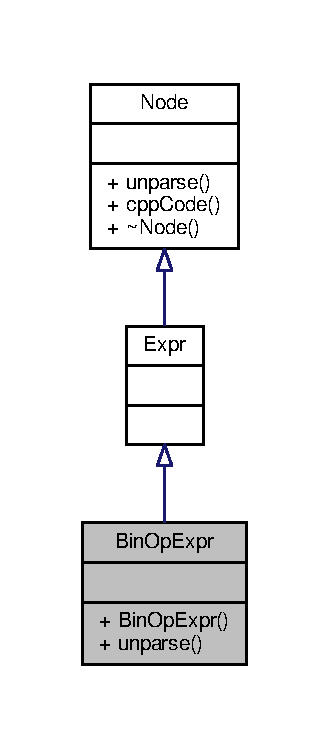
\includegraphics[width=158pt]{classBinOpExpr__inherit__graph}
\end{center}
\end{figure}


Collaboration diagram for Bin\-Op\-Expr\-:\nopagebreak
\begin{figure}[H]
\begin{center}
\leavevmode
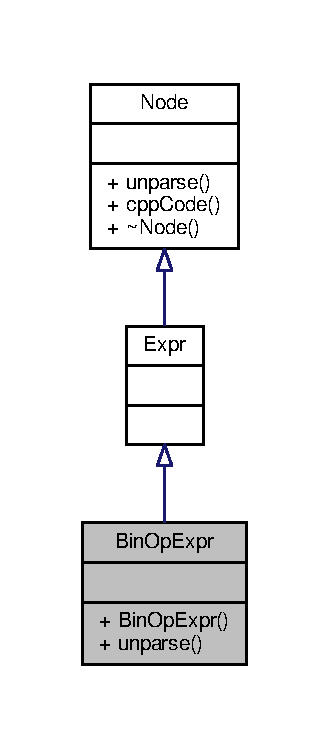
\includegraphics[width=158pt]{classBinOpExpr__coll__graph}
\end{center}
\end{figure}
\subsection*{Public Member Functions}
\begin{DoxyCompactItemize}
\item 
\hyperlink{classBinOpExpr_a1f1e3308250be423314a06f916a653c5}{Bin\-Op\-Expr} (\hyperlink{classExpr}{Expr} $\ast$L, std\-::string op, \hyperlink{classExpr}{Expr} $\ast$R)
\item 
std\-::string \hyperlink{classBinOpExpr_a1ec35159c20a6b8481ee89ae5829c14d}{unparse} ()
\begin{DoxyCompactList}\small\item\em Returns a string representation of the code modeled by this class and all its variables. \end{DoxyCompactList}\end{DoxyCompactItemize}


\subsection{Detailed Description}
Represents two expressions separated by an operation. \par
 

Model\-: \hyperlink{classExpr}{Expr} \-:\-:= \hyperlink{classExpr}{Expr} {\itshape op} \hyperlink{classExpr}{Expr} \par
 Example\-: 1 + 1 

\subsection{Constructor \& Destructor Documentation}
\hypertarget{classBinOpExpr_a1f1e3308250be423314a06f916a653c5}{\index{Bin\-Op\-Expr@{Bin\-Op\-Expr}!Bin\-Op\-Expr@{Bin\-Op\-Expr}}
\index{Bin\-Op\-Expr@{Bin\-Op\-Expr}!BinOpExpr@{Bin\-Op\-Expr}}
\subsubsection[{Bin\-Op\-Expr}]{\setlength{\rightskip}{0pt plus 5cm}Bin\-Op\-Expr\-::\-Bin\-Op\-Expr (
\begin{DoxyParamCaption}
\item[{{\bf Expr} $\ast$}]{L, }
\item[{std\-::string}]{op, }
\item[{{\bf Expr} $\ast$}]{R}
\end{DoxyParamCaption}
)\hspace{0.3cm}{\ttfamily [inline]}}}\label{classBinOpExpr_a1f1e3308250be423314a06f916a653c5}
Public constructor. 
\begin{DoxyParams}{Parameters}
{\em L} & -\/ Expression on left-\/hand side of operation \\
\hline
{\em op} & -\/ Operation splitting the left and right expressions \\
\hline
{\em R} & -\/ Expression on right-\/hand side of operation \\
\hline
\end{DoxyParams}


\subsection{Member Function Documentation}
\hypertarget{classBinOpExpr_a1ec35159c20a6b8481ee89ae5829c14d}{\index{Bin\-Op\-Expr@{Bin\-Op\-Expr}!unparse@{unparse}}
\index{unparse@{unparse}!BinOpExpr@{Bin\-Op\-Expr}}
\subsubsection[{unparse}]{\setlength{\rightskip}{0pt plus 5cm}string Bin\-Op\-Expr\-::unparse (
\begin{DoxyParamCaption}
{}
\end{DoxyParamCaption}
)\hspace{0.3cm}{\ttfamily [virtual]}}}\label{classBinOpExpr_a1ec35159c20a6b8481ee89ae5829c14d}


Returns a string representation of the code modeled by this class and all its variables. 

\begin{DoxyReturn}{Returns}
std\-::string. 
\end{DoxyReturn}


Implements \hyperlink{classNode_a60ea533e0900961c05e701db70097136}{Node}.



The documentation for this class was generated from the following files\-:\begin{DoxyCompactItemize}
\item 
\hyperlink{AST_8h}{A\-S\-T.\-h}\item 
\hyperlink{AST_8cpp}{A\-S\-T.\-cpp}\end{DoxyCompactItemize}

\hypertarget{classCharConstToken}{\section{Char\-Const\-Token Class Reference}
\label{classCharConstToken}\index{Char\-Const\-Token@{Char\-Const\-Token}}
}


{\ttfamily \#include $<$ext\-Token.\-h$>$}



Inheritance diagram for Char\-Const\-Token\-:\nopagebreak
\begin{figure}[H]
\begin{center}
\leavevmode
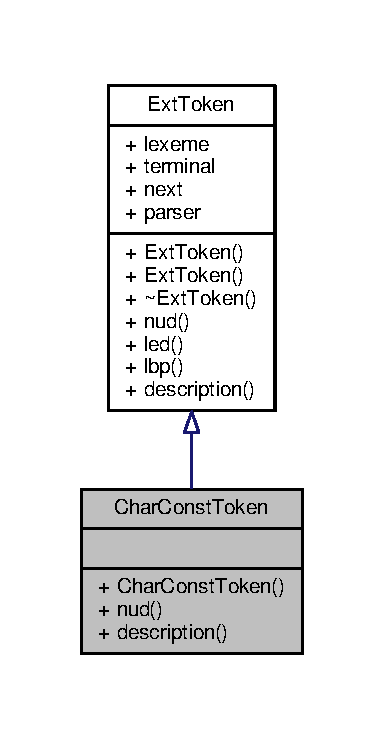
\includegraphics[width=184pt]{classCharConstToken__inherit__graph}
\end{center}
\end{figure}


Collaboration diagram for Char\-Const\-Token\-:\nopagebreak
\begin{figure}[H]
\begin{center}
\leavevmode
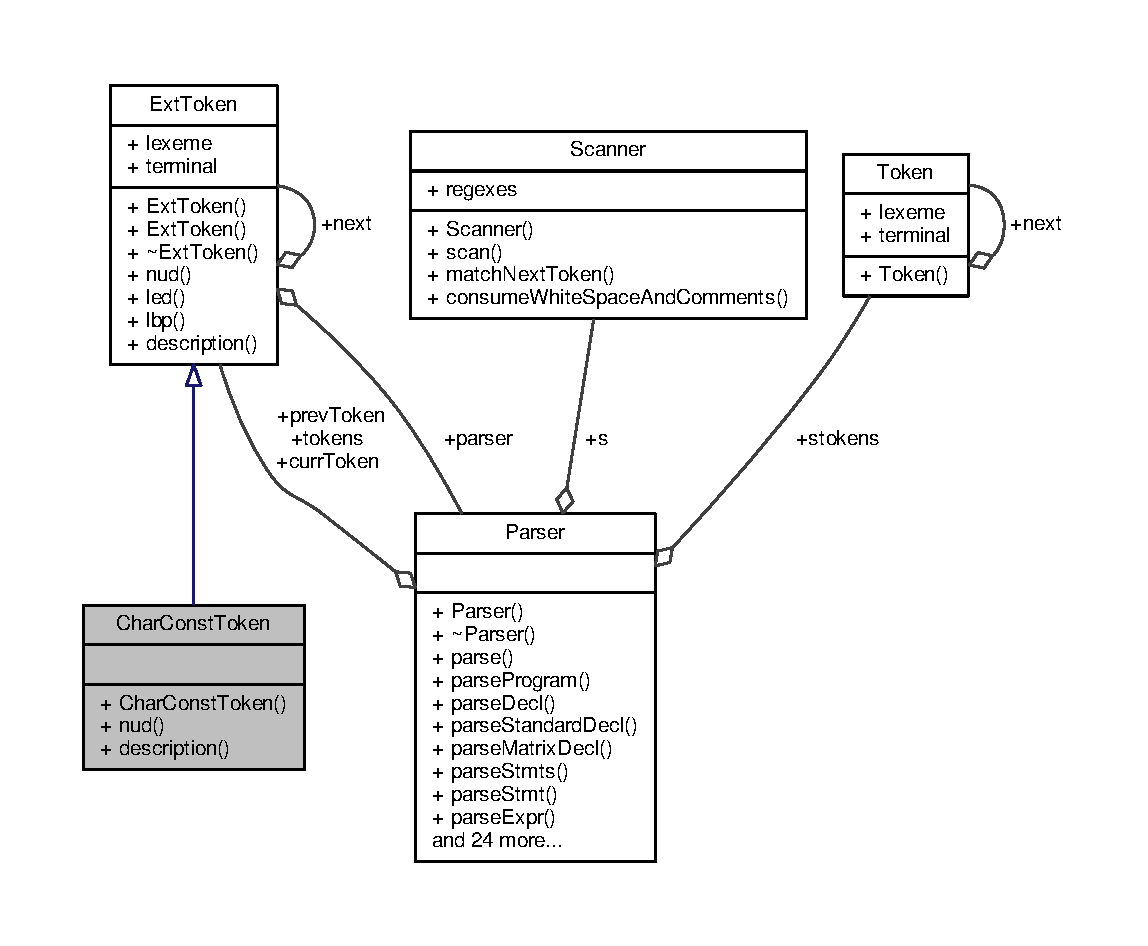
\includegraphics[width=350pt]{classCharConstToken__coll__graph}
\end{center}
\end{figure}
\subsection*{Public Member Functions}
\begin{DoxyCompactItemize}
\item 
\hyperlink{classCharConstToken_a9dcb8d0d26c4f9c66570357641933c51}{Char\-Const\-Token} (\hyperlink{classParser}{Parser} $\ast$p, \hyperlink{classToken}{Token} $\ast$t)
\item 
\hyperlink{classParseResult}{Parse\-Result} \hyperlink{classCharConstToken_a33032d6b35ef2b6ebc4db770b374ad5b}{nud} ()
\item 
std\-::string \hyperlink{classCharConstToken_addf2603d51bc2be908137f06737d8b30}{description} ()
\end{DoxyCompactItemize}
\subsection*{Additional Inherited Members}


\subsection{Constructor \& Destructor Documentation}
\hypertarget{classCharConstToken_a9dcb8d0d26c4f9c66570357641933c51}{\index{Char\-Const\-Token@{Char\-Const\-Token}!Char\-Const\-Token@{Char\-Const\-Token}}
\index{Char\-Const\-Token@{Char\-Const\-Token}!CharConstToken@{Char\-Const\-Token}}
\subsubsection[{Char\-Const\-Token}]{\setlength{\rightskip}{0pt plus 5cm}Char\-Const\-Token\-::\-Char\-Const\-Token (
\begin{DoxyParamCaption}
\item[{{\bf Parser} $\ast$}]{p, }
\item[{{\bf Token} $\ast$}]{t}
\end{DoxyParamCaption}
)\hspace{0.3cm}{\ttfamily [inline]}}}\label{classCharConstToken_a9dcb8d0d26c4f9c66570357641933c51}


\subsection{Member Function Documentation}
\hypertarget{classCharConstToken_addf2603d51bc2be908137f06737d8b30}{\index{Char\-Const\-Token@{Char\-Const\-Token}!description@{description}}
\index{description@{description}!CharConstToken@{Char\-Const\-Token}}
\subsubsection[{description}]{\setlength{\rightskip}{0pt plus 5cm}std\-::string Char\-Const\-Token\-::description (
\begin{DoxyParamCaption}
{}
\end{DoxyParamCaption}
)\hspace{0.3cm}{\ttfamily [inline]}, {\ttfamily [virtual]}}}\label{classCharConstToken_addf2603d51bc2be908137f06737d8b30}


Reimplemented from \hyperlink{classExtToken_a4ab6e72ac23235650b1756f794172ebb}{Ext\-Token}.

\hypertarget{classCharConstToken_a33032d6b35ef2b6ebc4db770b374ad5b}{\index{Char\-Const\-Token@{Char\-Const\-Token}!nud@{nud}}
\index{nud@{nud}!CharConstToken@{Char\-Const\-Token}}
\subsubsection[{nud}]{\setlength{\rightskip}{0pt plus 5cm}{\bf Parse\-Result} Char\-Const\-Token\-::nud (
\begin{DoxyParamCaption}
{}
\end{DoxyParamCaption}
)\hspace{0.3cm}{\ttfamily [inline]}, {\ttfamily [virtual]}}}\label{classCharConstToken_a33032d6b35ef2b6ebc4db770b374ad5b}


Reimplemented from \hyperlink{classExtToken_a5c21a5ffe91f212085259126652ab77c}{Ext\-Token}.



The documentation for this class was generated from the following file\-:\begin{DoxyCompactItemize}
\item 
\hyperlink{extToken_8h}{ext\-Token.\-h}\end{DoxyCompactItemize}

\hypertarget{classDashToken}{\section{Dash\-Token Class Reference}
\label{classDashToken}\index{Dash\-Token@{Dash\-Token}}
}


{\ttfamily \#include $<$ext\-Token.\-h$>$}



Inheritance diagram for Dash\-Token\-:\nopagebreak
\begin{figure}[H]
\begin{center}
\leavevmode
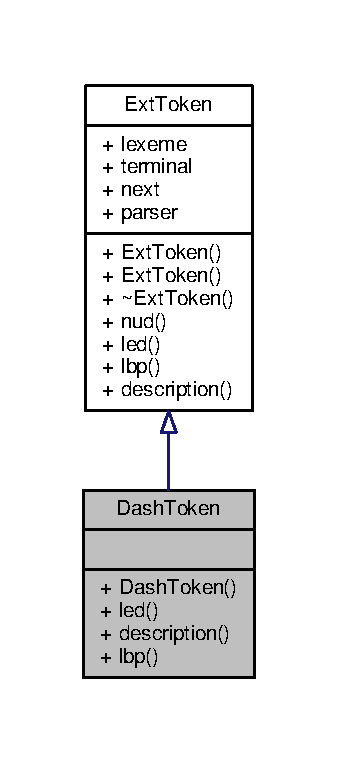
\includegraphics[width=162pt]{classDashToken__inherit__graph}
\end{center}
\end{figure}


Collaboration diagram for Dash\-Token\-:\nopagebreak
\begin{figure}[H]
\begin{center}
\leavevmode
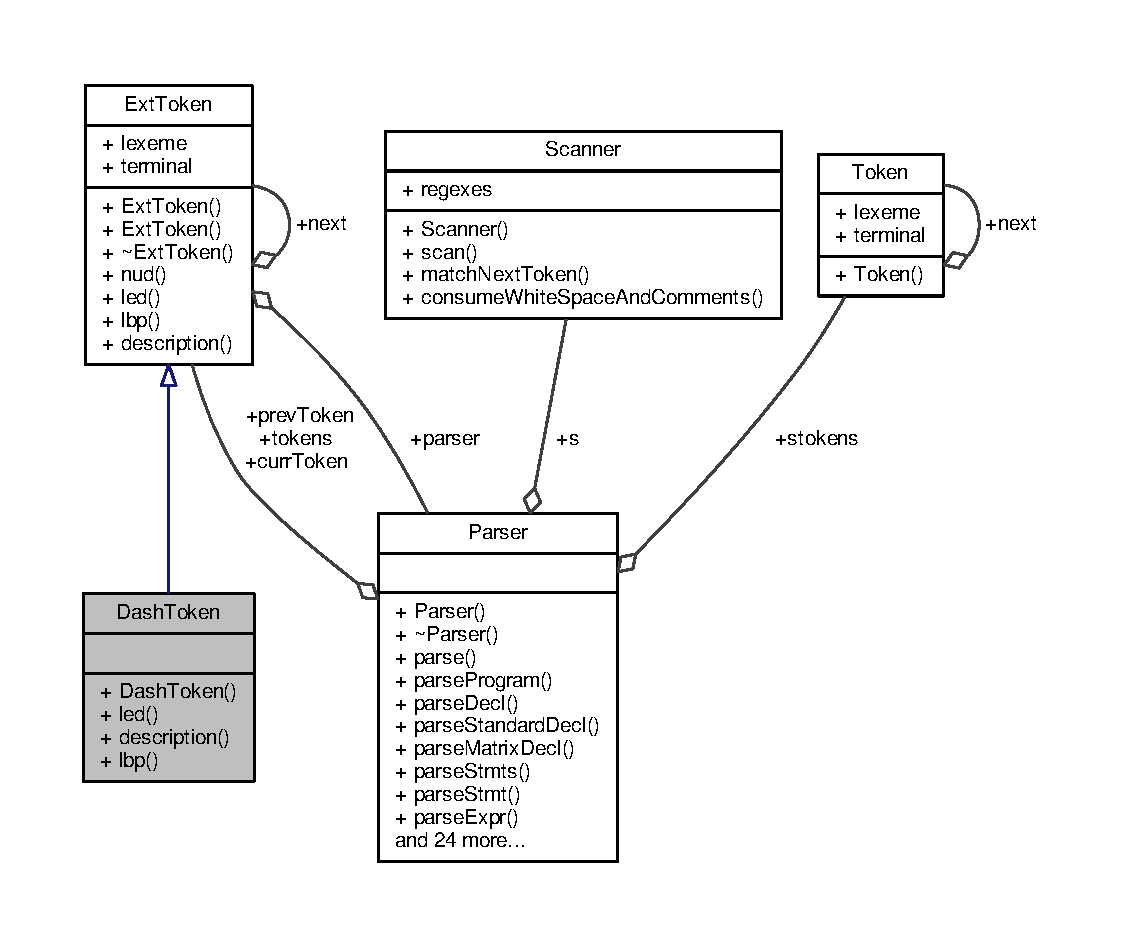
\includegraphics[width=350pt]{classDashToken__coll__graph}
\end{center}
\end{figure}
\subsection*{Public Member Functions}
\begin{DoxyCompactItemize}
\item 
\hyperlink{classDashToken_a9570d66563405c728e679b63a44e53e2}{Dash\-Token} (\hyperlink{classParser}{Parser} $\ast$p, \hyperlink{classToken}{Token} $\ast$t)
\item 
\hyperlink{classParseResult}{Parse\-Result} \hyperlink{classDashToken_a703ca6afcd05ac4688c66b82e177bdbc}{led} (\hyperlink{classParseResult}{Parse\-Result} left)
\item 
std\-::string \hyperlink{classDashToken_a02d79abb30dcab20081edb8e969885d2}{description} ()
\item 
int \hyperlink{classDashToken_a1cf877584a85c06e884a182744e92b39}{lbp} ()
\end{DoxyCompactItemize}
\subsection*{Additional Inherited Members}


\subsection{Constructor \& Destructor Documentation}
\hypertarget{classDashToken_a9570d66563405c728e679b63a44e53e2}{\index{Dash\-Token@{Dash\-Token}!Dash\-Token@{Dash\-Token}}
\index{Dash\-Token@{Dash\-Token}!DashToken@{Dash\-Token}}
\subsubsection[{Dash\-Token}]{\setlength{\rightskip}{0pt plus 5cm}Dash\-Token\-::\-Dash\-Token (
\begin{DoxyParamCaption}
\item[{{\bf Parser} $\ast$}]{p, }
\item[{{\bf Token} $\ast$}]{t}
\end{DoxyParamCaption}
)\hspace{0.3cm}{\ttfamily [inline]}}}\label{classDashToken_a9570d66563405c728e679b63a44e53e2}


\subsection{Member Function Documentation}
\hypertarget{classDashToken_a02d79abb30dcab20081edb8e969885d2}{\index{Dash\-Token@{Dash\-Token}!description@{description}}
\index{description@{description}!DashToken@{Dash\-Token}}
\subsubsection[{description}]{\setlength{\rightskip}{0pt plus 5cm}std\-::string Dash\-Token\-::description (
\begin{DoxyParamCaption}
{}
\end{DoxyParamCaption}
)\hspace{0.3cm}{\ttfamily [inline]}, {\ttfamily [virtual]}}}\label{classDashToken_a02d79abb30dcab20081edb8e969885d2}


Reimplemented from \hyperlink{classExtToken_a4ab6e72ac23235650b1756f794172ebb}{Ext\-Token}.

\hypertarget{classDashToken_a1cf877584a85c06e884a182744e92b39}{\index{Dash\-Token@{Dash\-Token}!lbp@{lbp}}
\index{lbp@{lbp}!DashToken@{Dash\-Token}}
\subsubsection[{lbp}]{\setlength{\rightskip}{0pt plus 5cm}int Dash\-Token\-::lbp (
\begin{DoxyParamCaption}
{}
\end{DoxyParamCaption}
)\hspace{0.3cm}{\ttfamily [inline]}, {\ttfamily [virtual]}}}\label{classDashToken_a1cf877584a85c06e884a182744e92b39}


Reimplemented from \hyperlink{classExtToken_a6c0d61faa058b71147dd54bacee1db94}{Ext\-Token}.

\hypertarget{classDashToken_a703ca6afcd05ac4688c66b82e177bdbc}{\index{Dash\-Token@{Dash\-Token}!led@{led}}
\index{led@{led}!DashToken@{Dash\-Token}}
\subsubsection[{led}]{\setlength{\rightskip}{0pt plus 5cm}{\bf Parse\-Result} Dash\-Token\-::led (
\begin{DoxyParamCaption}
\item[{{\bf Parse\-Result}}]{left}
\end{DoxyParamCaption}
)\hspace{0.3cm}{\ttfamily [inline]}, {\ttfamily [virtual]}}}\label{classDashToken_a703ca6afcd05ac4688c66b82e177bdbc}


Reimplemented from \hyperlink{classExtToken_afb2c9b0040e198d1d8aa2e041c5a7211}{Ext\-Token}.



The documentation for this class was generated from the following file\-:\begin{DoxyCompactItemize}
\item 
\hyperlink{extToken_8h}{ext\-Token.\-h}\end{DoxyCompactItemize}

\hypertarget{classEmptyStmts}{\section{Empty\-Stmts Class Reference}
\label{classEmptyStmts}\index{Empty\-Stmts@{Empty\-Stmts}}
}


Represents emptiness.  




{\ttfamily \#include $<$A\-S\-T.\-h$>$}



Inheritance diagram for Empty\-Stmts\-:\nopagebreak
\begin{figure}[H]
\begin{center}
\leavevmode
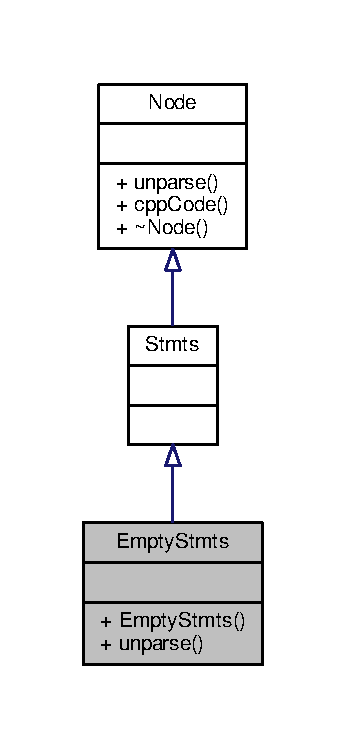
\includegraphics[width=166pt]{classEmptyStmts__inherit__graph}
\end{center}
\end{figure}


Collaboration diagram for Empty\-Stmts\-:\nopagebreak
\begin{figure}[H]
\begin{center}
\leavevmode
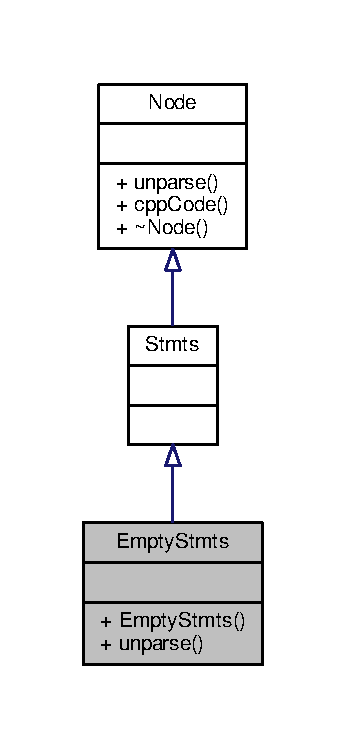
\includegraphics[width=166pt]{classEmptyStmts__coll__graph}
\end{center}
\end{figure}
\subsection*{Public Member Functions}
\begin{DoxyCompactItemize}
\item 
\hyperlink{classEmptyStmts_aec1fdeb62d294b8fedf55ff234fcacf5}{Empty\-Stmts} ()
\item 
std\-::string \hyperlink{classEmptyStmts_a0f5a1640891e7c70f8ac38d6df031f0e}{unparse} ()
\begin{DoxyCompactList}\small\item\em Returns a string representation of the code modeled by this class and all its variables. \end{DoxyCompactList}\end{DoxyCompactItemize}


\subsection{Detailed Description}
Represents emptiness. 

Model\-: \hyperlink{classStmts}{Stmts} \-:\-:= $<$$<$empty$>$$>$ \par
 Example\-: $<$$<$emptiness$>$$>$ 

\subsection{Constructor \& Destructor Documentation}
\hypertarget{classEmptyStmts_aec1fdeb62d294b8fedf55ff234fcacf5}{\index{Empty\-Stmts@{Empty\-Stmts}!Empty\-Stmts@{Empty\-Stmts}}
\index{Empty\-Stmts@{Empty\-Stmts}!EmptyStmts@{Empty\-Stmts}}
\subsubsection[{Empty\-Stmts}]{\setlength{\rightskip}{0pt plus 5cm}Empty\-Stmts\-::\-Empty\-Stmts (
\begin{DoxyParamCaption}
{}
\end{DoxyParamCaption}
)\hspace{0.3cm}{\ttfamily [inline]}}}\label{classEmptyStmts_aec1fdeb62d294b8fedf55ff234fcacf5}
Public constructor. 

\subsection{Member Function Documentation}
\hypertarget{classEmptyStmts_a0f5a1640891e7c70f8ac38d6df031f0e}{\index{Empty\-Stmts@{Empty\-Stmts}!unparse@{unparse}}
\index{unparse@{unparse}!EmptyStmts@{Empty\-Stmts}}
\subsubsection[{unparse}]{\setlength{\rightskip}{0pt plus 5cm}string Empty\-Stmts\-::unparse (
\begin{DoxyParamCaption}
{}
\end{DoxyParamCaption}
)\hspace{0.3cm}{\ttfamily [virtual]}}}\label{classEmptyStmts_a0f5a1640891e7c70f8ac38d6df031f0e}


Returns a string representation of the code modeled by this class and all its variables. 

\begin{DoxyReturn}{Returns}
std\-::string. 
\end{DoxyReturn}


Implements \hyperlink{classNode_a60ea533e0900961c05e701db70097136}{Node}.



The documentation for this class was generated from the following files\-:\begin{DoxyCompactItemize}
\item 
\hyperlink{AST_8h}{A\-S\-T.\-h}\item 
\hyperlink{AST_8cpp}{A\-S\-T.\-cpp}\end{DoxyCompactItemize}

\hypertarget{classEndOfFileToken}{\section{End\-Of\-File\-Token Class Reference}
\label{classEndOfFileToken}\index{End\-Of\-File\-Token@{End\-Of\-File\-Token}}
}


{\ttfamily \#include $<$ext\-Token.\-h$>$}



Inheritance diagram for End\-Of\-File\-Token\-:\nopagebreak
\begin{figure}[H]
\begin{center}
\leavevmode
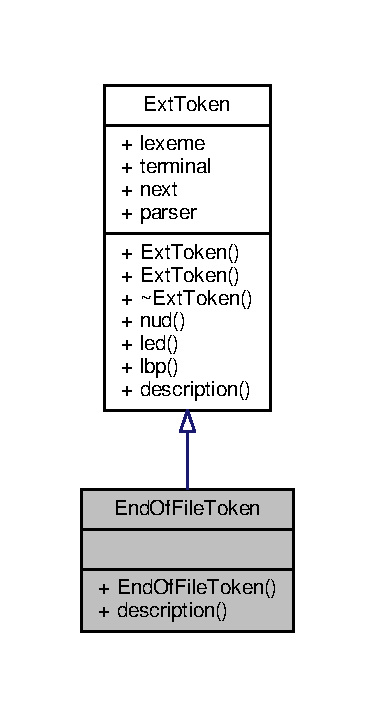
\includegraphics[width=180pt]{classEndOfFileToken__inherit__graph}
\end{center}
\end{figure}


Collaboration diagram for End\-Of\-File\-Token\-:\nopagebreak
\begin{figure}[H]
\begin{center}
\leavevmode
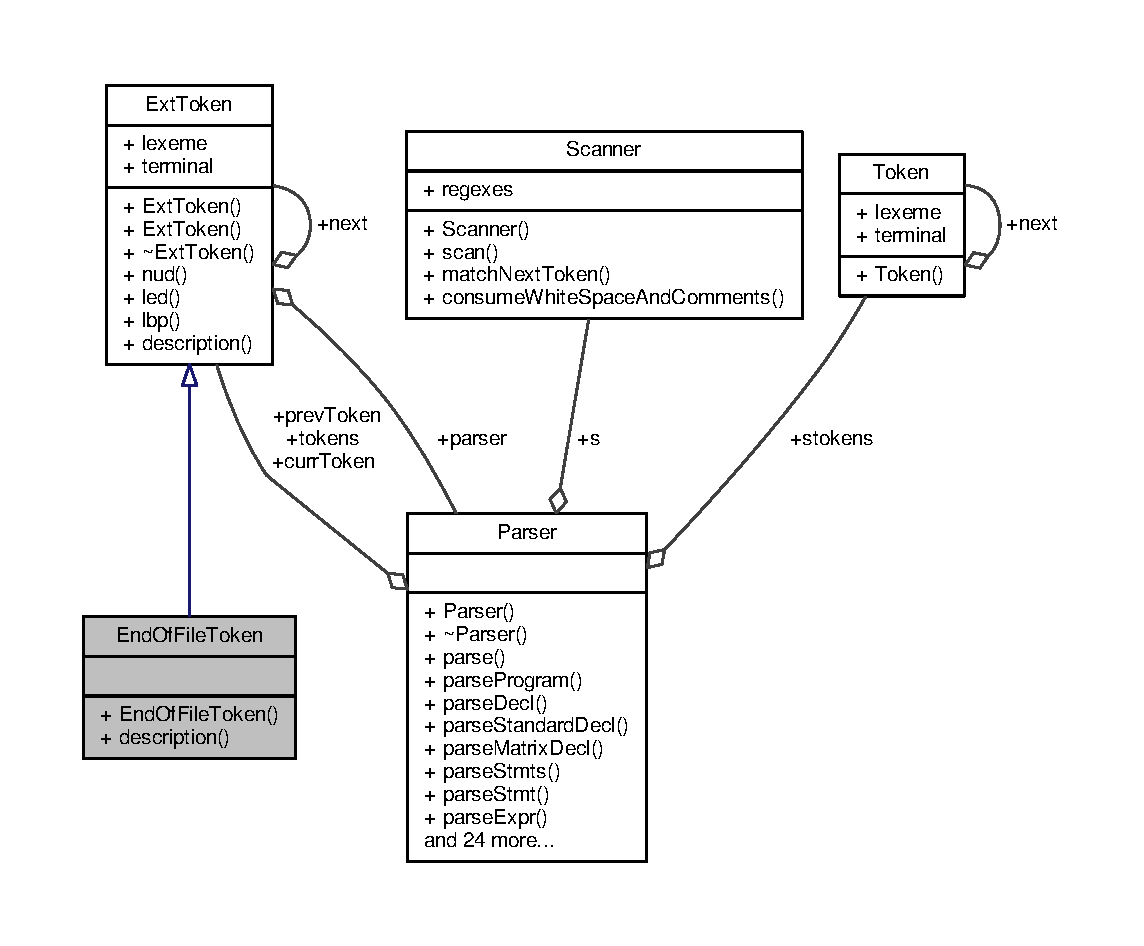
\includegraphics[width=350pt]{classEndOfFileToken__coll__graph}
\end{center}
\end{figure}
\subsection*{Public Member Functions}
\begin{DoxyCompactItemize}
\item 
\hyperlink{classEndOfFileToken_a5c093bc13648a4f4df525ea4242e59d9}{End\-Of\-File\-Token} (\hyperlink{classParser}{Parser} $\ast$p, \hyperlink{classToken}{Token} $\ast$t)
\item 
std\-::string \hyperlink{classEndOfFileToken_a918312b101ca8cc7fb5ba4e56bc12b58}{description} ()
\end{DoxyCompactItemize}
\subsection*{Additional Inherited Members}


\subsection{Constructor \& Destructor Documentation}
\hypertarget{classEndOfFileToken_a5c093bc13648a4f4df525ea4242e59d9}{\index{End\-Of\-File\-Token@{End\-Of\-File\-Token}!End\-Of\-File\-Token@{End\-Of\-File\-Token}}
\index{End\-Of\-File\-Token@{End\-Of\-File\-Token}!EndOfFileToken@{End\-Of\-File\-Token}}
\subsubsection[{End\-Of\-File\-Token}]{\setlength{\rightskip}{0pt plus 5cm}End\-Of\-File\-Token\-::\-End\-Of\-File\-Token (
\begin{DoxyParamCaption}
\item[{{\bf Parser} $\ast$}]{p, }
\item[{{\bf Token} $\ast$}]{t}
\end{DoxyParamCaption}
)\hspace{0.3cm}{\ttfamily [inline]}}}\label{classEndOfFileToken_a5c093bc13648a4f4df525ea4242e59d9}


\subsection{Member Function Documentation}
\hypertarget{classEndOfFileToken_a918312b101ca8cc7fb5ba4e56bc12b58}{\index{End\-Of\-File\-Token@{End\-Of\-File\-Token}!description@{description}}
\index{description@{description}!EndOfFileToken@{End\-Of\-File\-Token}}
\subsubsection[{description}]{\setlength{\rightskip}{0pt plus 5cm}std\-::string End\-Of\-File\-Token\-::description (
\begin{DoxyParamCaption}
{}
\end{DoxyParamCaption}
)\hspace{0.3cm}{\ttfamily [inline]}, {\ttfamily [virtual]}}}\label{classEndOfFileToken_a918312b101ca8cc7fb5ba4e56bc12b58}


Reimplemented from \hyperlink{classExtToken_a4ab6e72ac23235650b1756f794172ebb}{Ext\-Token}.



The documentation for this class was generated from the following file\-:\begin{DoxyCompactItemize}
\item 
\hyperlink{extToken_8h}{ext\-Token.\-h}\end{DoxyCompactItemize}

\hypertarget{classExpr}{\section{Expr Class Reference}
\label{classExpr}\index{Expr@{Expr}}
}


Parent for all expression instances to be parsed \par
  




{\ttfamily \#include $<$A\-S\-T.\-h$>$}



Inheritance diagram for Expr\-:\nopagebreak
\begin{figure}[H]
\begin{center}
\leavevmode
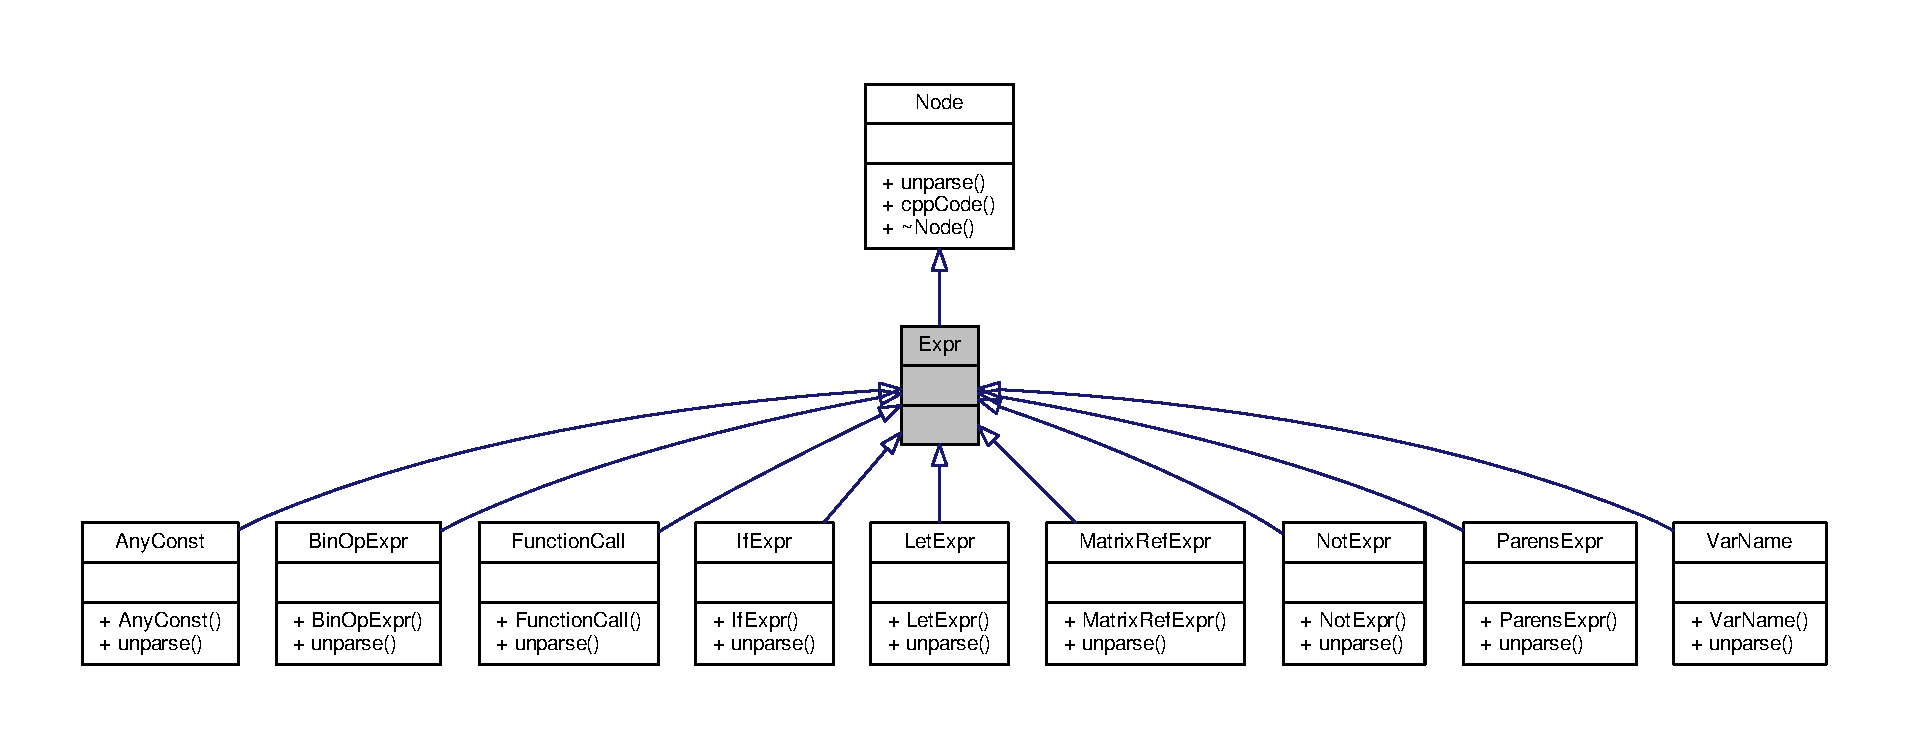
\includegraphics[width=350pt]{classExpr__inherit__graph}
\end{center}
\end{figure}


Collaboration diagram for Expr\-:\nopagebreak
\begin{figure}[H]
\begin{center}
\leavevmode
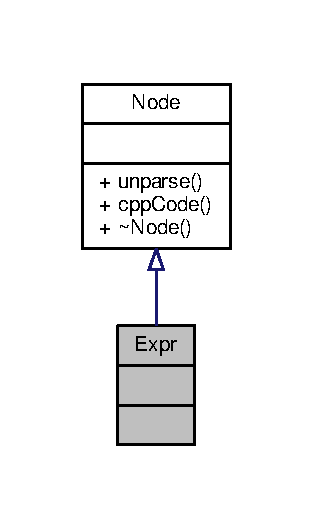
\includegraphics[width=150pt]{classExpr__coll__graph}
\end{center}
\end{figure}
\subsection*{Additional Inherited Members}


\subsection{Detailed Description}
Parent for all expression instances to be parsed \par
 

Model\-: \hyperlink{classExpr}{Expr} \-:\-:= var\-Name \par
 Example\-: x 

The documentation for this class was generated from the following file\-:\begin{DoxyCompactItemize}
\item 
\hyperlink{AST_8h}{A\-S\-T.\-h}\end{DoxyCompactItemize}

\hypertarget{classExtToken}{\section{Ext\-Token Class Reference}
\label{classExtToken}\index{Ext\-Token@{Ext\-Token}}
}


{\ttfamily \#include $<$ext\-Token.\-h$>$}



Inheritance diagram for Ext\-Token\-:\nopagebreak
\begin{figure}[H]
\begin{center}
\leavevmode
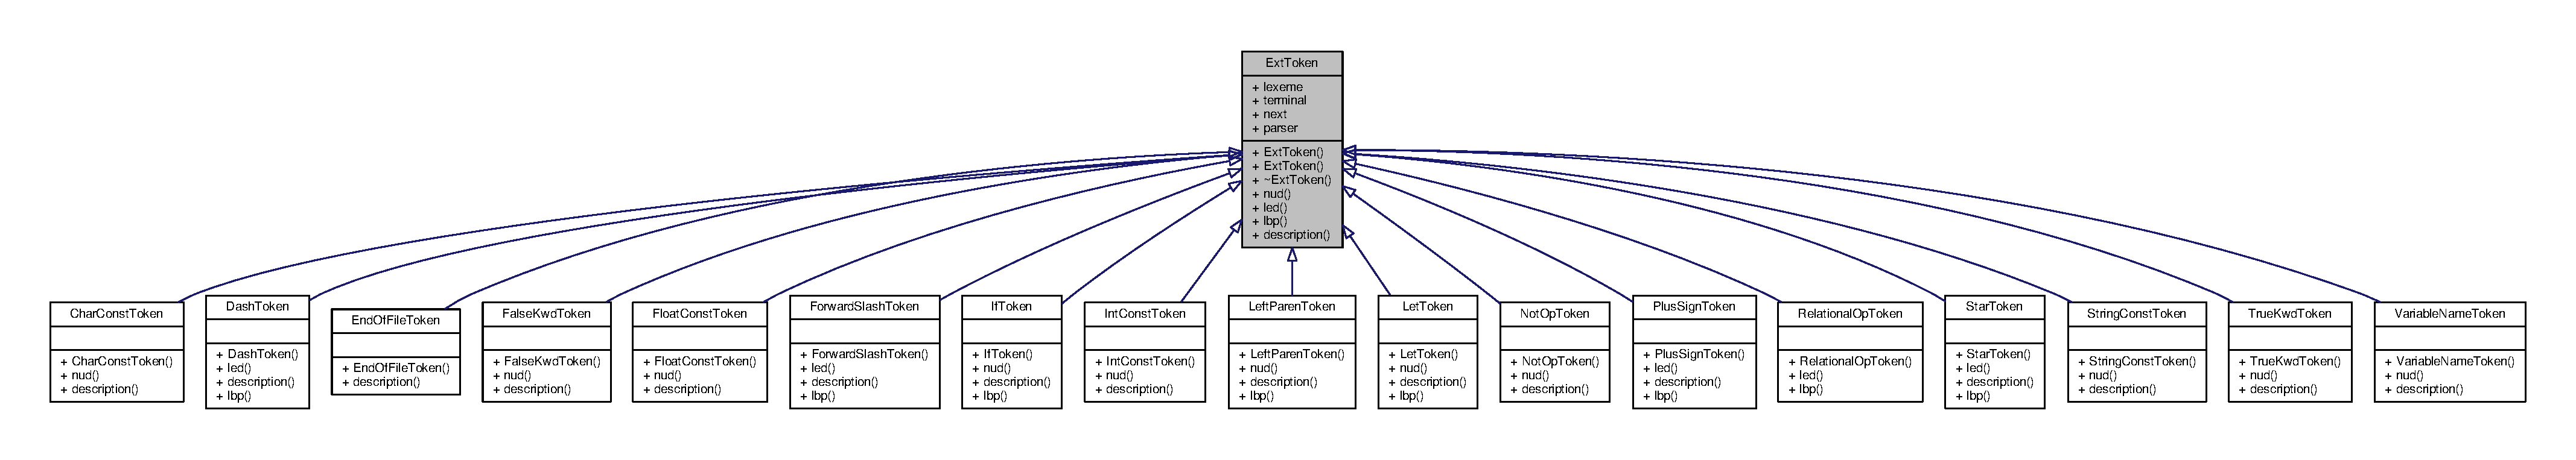
\includegraphics[width=350pt]{classExtToken__inherit__graph}
\end{center}
\end{figure}


Collaboration diagram for Ext\-Token\-:\nopagebreak
\begin{figure}[H]
\begin{center}
\leavevmode
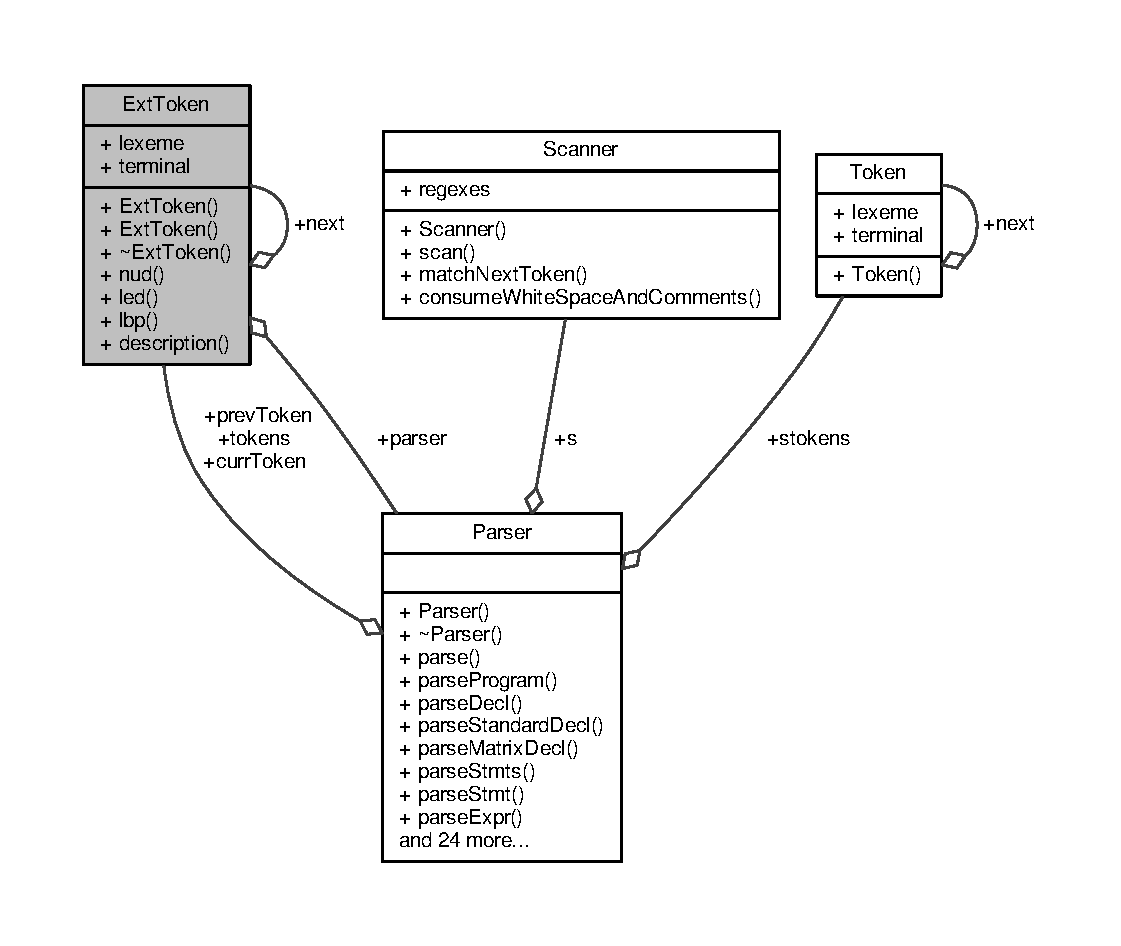
\includegraphics[width=350pt]{classExtToken__coll__graph}
\end{center}
\end{figure}
\subsection*{Public Member Functions}
\begin{DoxyCompactItemize}
\item 
\hyperlink{classExtToken_a45a27528f391faf5679b7b30563ce846}{Ext\-Token} (\hyperlink{classParser}{Parser} $\ast$p, \hyperlink{classToken}{Token} $\ast$t)
\item 
\hyperlink{classExtToken_afa8972152abec42cd52b6f6f70a9a179}{Ext\-Token} (\hyperlink{classParser}{Parser} $\ast$p, \hyperlink{classToken}{Token} $\ast$t, std\-::string d)
\item 
virtual \hyperlink{classExtToken_a20af764e16aad213816429272d96a918}{$\sim$\-Ext\-Token} ()
\item 
virtual \hyperlink{classParseResult}{Parse\-Result} \hyperlink{classExtToken_a5c21a5ffe91f212085259126652ab77c}{nud} ()
\item 
virtual \hyperlink{classParseResult}{Parse\-Result} \hyperlink{classExtToken_afb2c9b0040e198d1d8aa2e041c5a7211}{led} (\hyperlink{classParseResult}{Parse\-Result} left)
\item 
virtual int \hyperlink{classExtToken_a6c0d61faa058b71147dd54bacee1db94}{lbp} ()
\item 
virtual std\-::string \hyperlink{classExtToken_a4ab6e72ac23235650b1756f794172ebb}{description} ()
\end{DoxyCompactItemize}
\subsection*{Public Attributes}
\begin{DoxyCompactItemize}
\item 
std\-::string \hyperlink{classExtToken_a5af1643a542ef7ee8ca0f82706383ae3}{lexeme}
\item 
\hyperlink{scanner_8h_ab7f9b765cab7ed98e5a7f05690f6a061}{token\-Type} \hyperlink{classExtToken_abbdaef42b65403cdc0247839ef95c875}{terminal}
\item 
\hyperlink{classExtToken}{Ext\-Token} $\ast$ \hyperlink{classExtToken_aa02995a897183b2a6ef758e541534e46}{next}
\item 
\hyperlink{classParser}{Parser} $\ast$ \hyperlink{classExtToken_af70d22156d5f8e855a8b0d92a82706ba}{parser}
\end{DoxyCompactItemize}


\subsection{Constructor \& Destructor Documentation}
\hypertarget{classExtToken_a45a27528f391faf5679b7b30563ce846}{\index{Ext\-Token@{Ext\-Token}!Ext\-Token@{Ext\-Token}}
\index{Ext\-Token@{Ext\-Token}!ExtToken@{Ext\-Token}}
\subsubsection[{Ext\-Token}]{\setlength{\rightskip}{0pt plus 5cm}Ext\-Token\-::\-Ext\-Token (
\begin{DoxyParamCaption}
\item[{{\bf Parser} $\ast$}]{p, }
\item[{{\bf Token} $\ast$}]{t}
\end{DoxyParamCaption}
)\hspace{0.3cm}{\ttfamily [inline]}}}\label{classExtToken_a45a27528f391faf5679b7b30563ce846}
\hypertarget{classExtToken_afa8972152abec42cd52b6f6f70a9a179}{\index{Ext\-Token@{Ext\-Token}!Ext\-Token@{Ext\-Token}}
\index{Ext\-Token@{Ext\-Token}!ExtToken@{Ext\-Token}}
\subsubsection[{Ext\-Token}]{\setlength{\rightskip}{0pt plus 5cm}Ext\-Token\-::\-Ext\-Token (
\begin{DoxyParamCaption}
\item[{{\bf Parser} $\ast$}]{p, }
\item[{{\bf Token} $\ast$}]{t, }
\item[{std\-::string}]{d}
\end{DoxyParamCaption}
)\hspace{0.3cm}{\ttfamily [inline]}}}\label{classExtToken_afa8972152abec42cd52b6f6f70a9a179}
\hypertarget{classExtToken_a20af764e16aad213816429272d96a918}{\index{Ext\-Token@{Ext\-Token}!$\sim$\-Ext\-Token@{$\sim$\-Ext\-Token}}
\index{$\sim$\-Ext\-Token@{$\sim$\-Ext\-Token}!ExtToken@{Ext\-Token}}
\subsubsection[{$\sim$\-Ext\-Token}]{\setlength{\rightskip}{0pt plus 5cm}virtual Ext\-Token\-::$\sim$\-Ext\-Token (
\begin{DoxyParamCaption}
{}
\end{DoxyParamCaption}
)\hspace{0.3cm}{\ttfamily [inline]}, {\ttfamily [virtual]}}}\label{classExtToken_a20af764e16aad213816429272d96a918}


\subsection{Member Function Documentation}
\hypertarget{classExtToken_a4ab6e72ac23235650b1756f794172ebb}{\index{Ext\-Token@{Ext\-Token}!description@{description}}
\index{description@{description}!ExtToken@{Ext\-Token}}
\subsubsection[{description}]{\setlength{\rightskip}{0pt plus 5cm}virtual std\-::string Ext\-Token\-::description (
\begin{DoxyParamCaption}
{}
\end{DoxyParamCaption}
)\hspace{0.3cm}{\ttfamily [inline]}, {\ttfamily [virtual]}}}\label{classExtToken_a4ab6e72ac23235650b1756f794172ebb}


Reimplemented in \hyperlink{classEndOfFileToken_a918312b101ca8cc7fb5ba4e56bc12b58}{End\-Of\-File\-Token}, \hyperlink{classForwardSlashToken_ac27b1ab175ec08c468bd0d4c41636a5c}{Forward\-Slash\-Token}, \hyperlink{classDashToken_a02d79abb30dcab20081edb8e969885d2}{Dash\-Token}, \hyperlink{classStarToken_a59b81cb08057d75eca4b9a8aad8e2be1}{Star\-Token}, \hyperlink{classPlusSignToken_a61a05ac9660848e13da97d5746808868}{Plus\-Sign\-Token}, \hyperlink{classLeftParenToken_a2df35684bd2081c3bdfe2357946917bc}{Left\-Paren\-Token}, \hyperlink{classLetToken_a2c5ba0489774bf6468a26f4e19d7fab4}{Let\-Token}, \hyperlink{classIfToken_aad226162c5649920c13c2a9e9e7a3617}{If\-Token}, \hyperlink{classVariableNameToken_a54bc3a78736e5c967dc4b1c58e66135b}{Variable\-Name\-Token}, \hyperlink{classCharConstToken_addf2603d51bc2be908137f06737d8b30}{Char\-Const\-Token}, \hyperlink{classStringConstToken_a6343169471a6cb6e422496f2f640691f}{String\-Const\-Token}, \hyperlink{classFloatConstToken_a529b6d3ad479b0f6b940a82ba48b98c0}{Float\-Const\-Token}, \hyperlink{classIntConstToken_a98191508d849878d40800e447a0f1892}{Int\-Const\-Token}, \hyperlink{classFalseKwdToken_a8351fad7090214687138e113b5a581f1}{False\-Kwd\-Token}, \hyperlink{classTrueKwdToken_af4dbe740f06e6928a436d06349af67a9}{True\-Kwd\-Token}, and \hyperlink{classNotOpToken_a136a11f1e42542a9a58b7c14249c9d23}{Not\-Op\-Token}.

\hypertarget{classExtToken_a6c0d61faa058b71147dd54bacee1db94}{\index{Ext\-Token@{Ext\-Token}!lbp@{lbp}}
\index{lbp@{lbp}!ExtToken@{Ext\-Token}}
\subsubsection[{lbp}]{\setlength{\rightskip}{0pt plus 5cm}virtual int Ext\-Token\-::lbp (
\begin{DoxyParamCaption}
{}
\end{DoxyParamCaption}
)\hspace{0.3cm}{\ttfamily [inline]}, {\ttfamily [virtual]}}}\label{classExtToken_a6c0d61faa058b71147dd54bacee1db94}


Reimplemented in \hyperlink{classRelationalOpToken_ada096491d9553aea21089230489d6aef}{Relational\-Op\-Token}, \hyperlink{classForwardSlashToken_ad65829044355922a291dfbfd3052b183}{Forward\-Slash\-Token}, \hyperlink{classDashToken_a1cf877584a85c06e884a182744e92b39}{Dash\-Token}, \hyperlink{classStarToken_a87682a46d434781795d060e43e7eae23}{Star\-Token}, \hyperlink{classPlusSignToken_a80753eec970928e042da350df83150f2}{Plus\-Sign\-Token}, \hyperlink{classLeftParenToken_afa1b94645278f097bb097d3b24445d14}{Left\-Paren\-Token}, \hyperlink{classLetToken_a2a5ab5bc5897340513480c162bb2b065}{Let\-Token}, and \hyperlink{classIfToken_abfd39ff4c4818d382bf0b97fd097c478}{If\-Token}.

\hypertarget{classExtToken_afb2c9b0040e198d1d8aa2e041c5a7211}{\index{Ext\-Token@{Ext\-Token}!led@{led}}
\index{led@{led}!ExtToken@{Ext\-Token}}
\subsubsection[{led}]{\setlength{\rightskip}{0pt plus 5cm}virtual {\bf Parse\-Result} Ext\-Token\-::led (
\begin{DoxyParamCaption}
\item[{{\bf Parse\-Result}}]{left}
\end{DoxyParamCaption}
)\hspace{0.3cm}{\ttfamily [inline]}, {\ttfamily [virtual]}}}\label{classExtToken_afb2c9b0040e198d1d8aa2e041c5a7211}


Reimplemented in \hyperlink{classRelationalOpToken_a426c64391e7b3272d8e6277964730e05}{Relational\-Op\-Token}, \hyperlink{classForwardSlashToken_ac2dda7b791ab555e4323f17baaf323e1}{Forward\-Slash\-Token}, \hyperlink{classDashToken_a703ca6afcd05ac4688c66b82e177bdbc}{Dash\-Token}, \hyperlink{classStarToken_aba82bdc81500a58096bfeedad600ad10}{Star\-Token}, and \hyperlink{classPlusSignToken_a4d79a17891f92800259308ce71402526}{Plus\-Sign\-Token}.

\hypertarget{classExtToken_a5c21a5ffe91f212085259126652ab77c}{\index{Ext\-Token@{Ext\-Token}!nud@{nud}}
\index{nud@{nud}!ExtToken@{Ext\-Token}}
\subsubsection[{nud}]{\setlength{\rightskip}{0pt plus 5cm}virtual {\bf Parse\-Result} Ext\-Token\-::nud (
\begin{DoxyParamCaption}
{}
\end{DoxyParamCaption}
)\hspace{0.3cm}{\ttfamily [inline]}, {\ttfamily [virtual]}}}\label{classExtToken_a5c21a5ffe91f212085259126652ab77c}


Reimplemented in \hyperlink{classLeftParenToken_a3cb3ae9ab2647e5534c85529d314f08b}{Left\-Paren\-Token}, \hyperlink{classLetToken_a14df948cdf775bde8392bf58d53b91f3}{Let\-Token}, \hyperlink{classIfToken_add06bd79ce755fd5503f78e507109e52}{If\-Token}, \hyperlink{classVariableNameToken_a6e775ad5b8c2eafd2e2a185ab90b1f27}{Variable\-Name\-Token}, \hyperlink{classCharConstToken_a33032d6b35ef2b6ebc4db770b374ad5b}{Char\-Const\-Token}, \hyperlink{classStringConstToken_a4767bba84d30289ab31d501f240b80fb}{String\-Const\-Token}, \hyperlink{classFloatConstToken_a991e92ae34d0b01a3b1dd08ed01b8e6e}{Float\-Const\-Token}, \hyperlink{classIntConstToken_ae1f720d6006c47e145cae7879d09c708}{Int\-Const\-Token}, \hyperlink{classFalseKwdToken_adc06b0433535d552c1e7f8076d756fb3}{False\-Kwd\-Token}, \hyperlink{classTrueKwdToken_ad86f05acb9483438db153eab44aa6dac}{True\-Kwd\-Token}, and \hyperlink{classNotOpToken_a55a0dd53742aaca04338c16be079b031}{Not\-Op\-Token}.



\subsection{Member Data Documentation}
\hypertarget{classExtToken_a5af1643a542ef7ee8ca0f82706383ae3}{\index{Ext\-Token@{Ext\-Token}!lexeme@{lexeme}}
\index{lexeme@{lexeme}!ExtToken@{Ext\-Token}}
\subsubsection[{lexeme}]{\setlength{\rightskip}{0pt plus 5cm}std\-::string Ext\-Token\-::lexeme}}\label{classExtToken_a5af1643a542ef7ee8ca0f82706383ae3}
\hypertarget{classExtToken_aa02995a897183b2a6ef758e541534e46}{\index{Ext\-Token@{Ext\-Token}!next@{next}}
\index{next@{next}!ExtToken@{Ext\-Token}}
\subsubsection[{next}]{\setlength{\rightskip}{0pt plus 5cm}{\bf Ext\-Token}$\ast$ Ext\-Token\-::next}}\label{classExtToken_aa02995a897183b2a6ef758e541534e46}
\hypertarget{classExtToken_af70d22156d5f8e855a8b0d92a82706ba}{\index{Ext\-Token@{Ext\-Token}!parser@{parser}}
\index{parser@{parser}!ExtToken@{Ext\-Token}}
\subsubsection[{parser}]{\setlength{\rightskip}{0pt plus 5cm}{\bf Parser}$\ast$ Ext\-Token\-::parser}}\label{classExtToken_af70d22156d5f8e855a8b0d92a82706ba}
\hypertarget{classExtToken_abbdaef42b65403cdc0247839ef95c875}{\index{Ext\-Token@{Ext\-Token}!terminal@{terminal}}
\index{terminal@{terminal}!ExtToken@{Ext\-Token}}
\subsubsection[{terminal}]{\setlength{\rightskip}{0pt plus 5cm}{\bf token\-Type} Ext\-Token\-::terminal}}\label{classExtToken_abbdaef42b65403cdc0247839ef95c875}


The documentation for this class was generated from the following file\-:\begin{DoxyCompactItemize}
\item 
\hyperlink{extToken_8h}{ext\-Token.\-h}\end{DoxyCompactItemize}

\hypertarget{classFalseKwdToken}{\section{False\-Kwd\-Token Class Reference}
\label{classFalseKwdToken}\index{False\-Kwd\-Token@{False\-Kwd\-Token}}
}


{\ttfamily \#include $<$ext\-Token.\-h$>$}



Inheritance diagram for False\-Kwd\-Token\-:\nopagebreak
\begin{figure}[H]
\begin{center}
\leavevmode
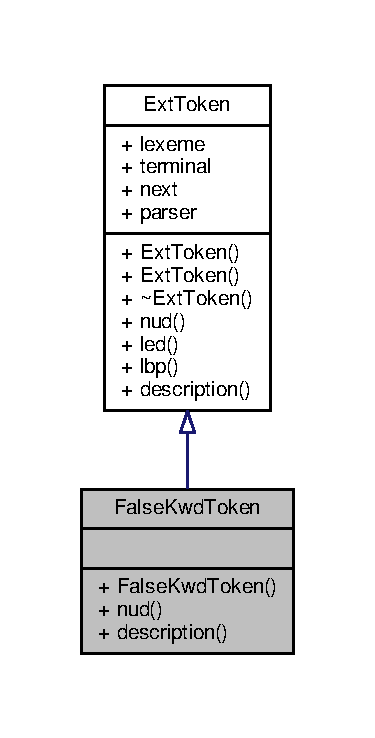
\includegraphics[width=180pt]{classFalseKwdToken__inherit__graph}
\end{center}
\end{figure}


Collaboration diagram for False\-Kwd\-Token\-:\nopagebreak
\begin{figure}[H]
\begin{center}
\leavevmode
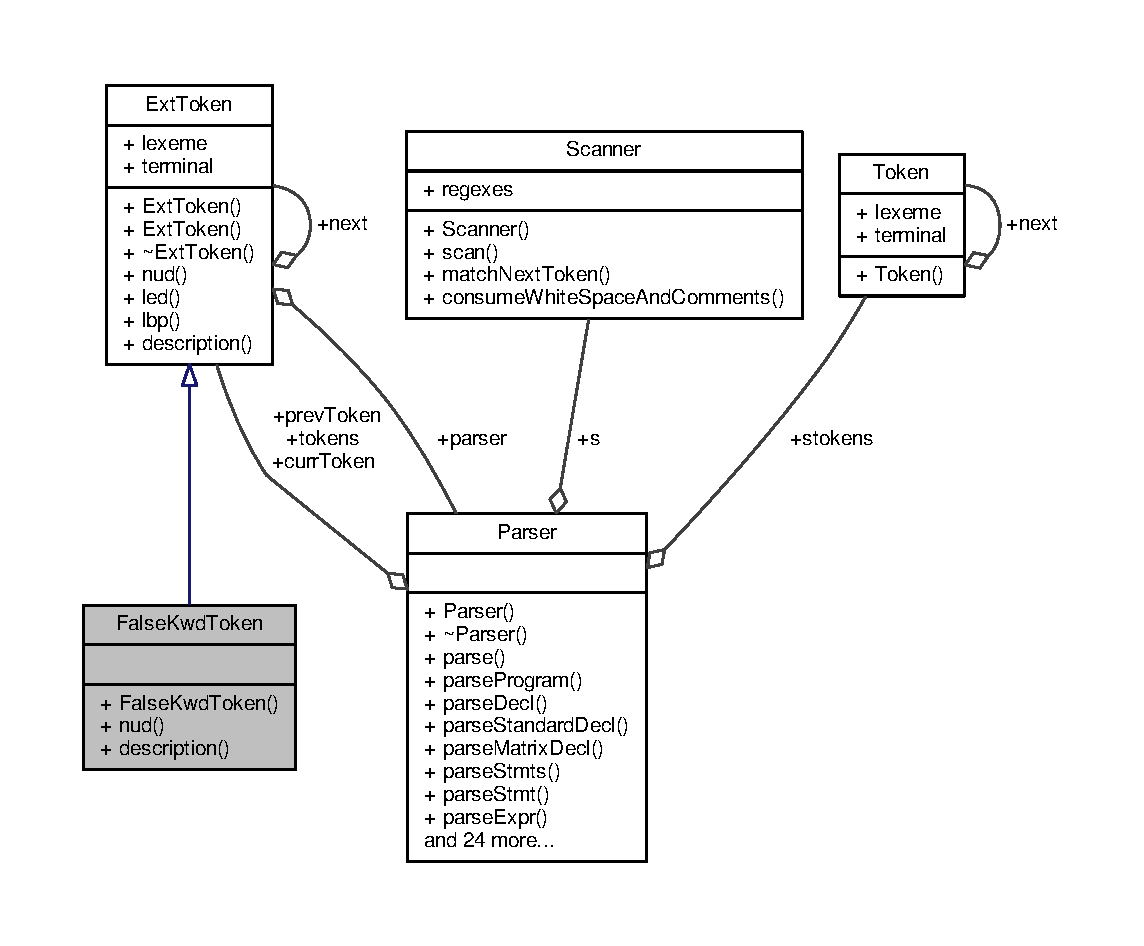
\includegraphics[width=350pt]{classFalseKwdToken__coll__graph}
\end{center}
\end{figure}
\subsection*{Public Member Functions}
\begin{DoxyCompactItemize}
\item 
\hyperlink{classFalseKwdToken_add6402d29fd7b22253a0dc73370597e4}{False\-Kwd\-Token} (\hyperlink{classParser}{Parser} $\ast$p, \hyperlink{classToken}{Token} $\ast$t)
\item 
\hyperlink{classParseResult}{Parse\-Result} \hyperlink{classFalseKwdToken_adc06b0433535d552c1e7f8076d756fb3}{nud} ()
\item 
std\-::string \hyperlink{classFalseKwdToken_a8351fad7090214687138e113b5a581f1}{description} ()
\end{DoxyCompactItemize}
\subsection*{Additional Inherited Members}


\subsection{Constructor \& Destructor Documentation}
\hypertarget{classFalseKwdToken_add6402d29fd7b22253a0dc73370597e4}{\index{False\-Kwd\-Token@{False\-Kwd\-Token}!False\-Kwd\-Token@{False\-Kwd\-Token}}
\index{False\-Kwd\-Token@{False\-Kwd\-Token}!FalseKwdToken@{False\-Kwd\-Token}}
\subsubsection[{False\-Kwd\-Token}]{\setlength{\rightskip}{0pt plus 5cm}False\-Kwd\-Token\-::\-False\-Kwd\-Token (
\begin{DoxyParamCaption}
\item[{{\bf Parser} $\ast$}]{p, }
\item[{{\bf Token} $\ast$}]{t}
\end{DoxyParamCaption}
)\hspace{0.3cm}{\ttfamily [inline]}}}\label{classFalseKwdToken_add6402d29fd7b22253a0dc73370597e4}


\subsection{Member Function Documentation}
\hypertarget{classFalseKwdToken_a8351fad7090214687138e113b5a581f1}{\index{False\-Kwd\-Token@{False\-Kwd\-Token}!description@{description}}
\index{description@{description}!FalseKwdToken@{False\-Kwd\-Token}}
\subsubsection[{description}]{\setlength{\rightskip}{0pt plus 5cm}std\-::string False\-Kwd\-Token\-::description (
\begin{DoxyParamCaption}
{}
\end{DoxyParamCaption}
)\hspace{0.3cm}{\ttfamily [inline]}, {\ttfamily [virtual]}}}\label{classFalseKwdToken_a8351fad7090214687138e113b5a581f1}


Reimplemented from \hyperlink{classExtToken_a4ab6e72ac23235650b1756f794172ebb}{Ext\-Token}.

\hypertarget{classFalseKwdToken_adc06b0433535d552c1e7f8076d756fb3}{\index{False\-Kwd\-Token@{False\-Kwd\-Token}!nud@{nud}}
\index{nud@{nud}!FalseKwdToken@{False\-Kwd\-Token}}
\subsubsection[{nud}]{\setlength{\rightskip}{0pt plus 5cm}{\bf Parse\-Result} False\-Kwd\-Token\-::nud (
\begin{DoxyParamCaption}
{}
\end{DoxyParamCaption}
)\hspace{0.3cm}{\ttfamily [inline]}, {\ttfamily [virtual]}}}\label{classFalseKwdToken_adc06b0433535d552c1e7f8076d756fb3}


Reimplemented from \hyperlink{classExtToken_a5c21a5ffe91f212085259126652ab77c}{Ext\-Token}.



The documentation for this class was generated from the following file\-:\begin{DoxyCompactItemize}
\item 
\hyperlink{extToken_8h}{ext\-Token.\-h}\end{DoxyCompactItemize}

\hypertarget{classFloatConstToken}{\section{Float\-Const\-Token Class Reference}
\label{classFloatConstToken}\index{Float\-Const\-Token@{Float\-Const\-Token}}
}


{\ttfamily \#include $<$ext\-Token.\-h$>$}



Inheritance diagram for Float\-Const\-Token\-:\nopagebreak
\begin{figure}[H]
\begin{center}
\leavevmode
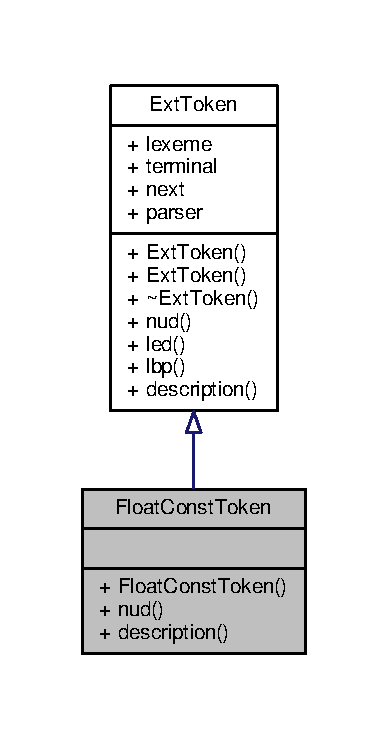
\includegraphics[width=186pt]{classFloatConstToken__inherit__graph}
\end{center}
\end{figure}


Collaboration diagram for Float\-Const\-Token\-:\nopagebreak
\begin{figure}[H]
\begin{center}
\leavevmode
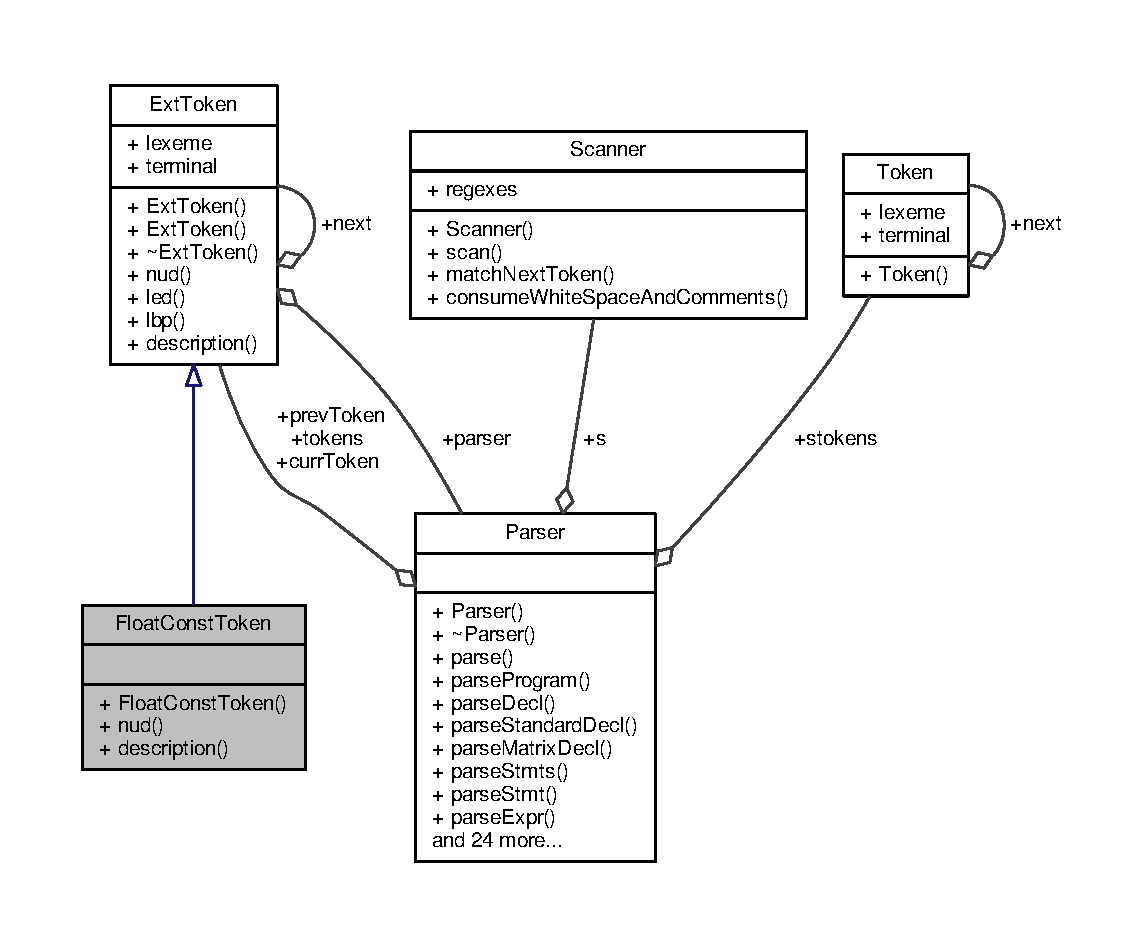
\includegraphics[width=350pt]{classFloatConstToken__coll__graph}
\end{center}
\end{figure}
\subsection*{Public Member Functions}
\begin{DoxyCompactItemize}
\item 
\hyperlink{classFloatConstToken_aecee1d0e4e8a9410701c68c30858a4db}{Float\-Const\-Token} (\hyperlink{classParser}{Parser} $\ast$p, \hyperlink{classToken}{Token} $\ast$t)
\item 
\hyperlink{classParseResult}{Parse\-Result} \hyperlink{classFloatConstToken_a991e92ae34d0b01a3b1dd08ed01b8e6e}{nud} ()
\item 
std\-::string \hyperlink{classFloatConstToken_a529b6d3ad479b0f6b940a82ba48b98c0}{description} ()
\end{DoxyCompactItemize}
\subsection*{Additional Inherited Members}


\subsection{Constructor \& Destructor Documentation}
\hypertarget{classFloatConstToken_aecee1d0e4e8a9410701c68c30858a4db}{\index{Float\-Const\-Token@{Float\-Const\-Token}!Float\-Const\-Token@{Float\-Const\-Token}}
\index{Float\-Const\-Token@{Float\-Const\-Token}!FloatConstToken@{Float\-Const\-Token}}
\subsubsection[{Float\-Const\-Token}]{\setlength{\rightskip}{0pt plus 5cm}Float\-Const\-Token\-::\-Float\-Const\-Token (
\begin{DoxyParamCaption}
\item[{{\bf Parser} $\ast$}]{p, }
\item[{{\bf Token} $\ast$}]{t}
\end{DoxyParamCaption}
)\hspace{0.3cm}{\ttfamily [inline]}}}\label{classFloatConstToken_aecee1d0e4e8a9410701c68c30858a4db}


\subsection{Member Function Documentation}
\hypertarget{classFloatConstToken_a529b6d3ad479b0f6b940a82ba48b98c0}{\index{Float\-Const\-Token@{Float\-Const\-Token}!description@{description}}
\index{description@{description}!FloatConstToken@{Float\-Const\-Token}}
\subsubsection[{description}]{\setlength{\rightskip}{0pt plus 5cm}std\-::string Float\-Const\-Token\-::description (
\begin{DoxyParamCaption}
{}
\end{DoxyParamCaption}
)\hspace{0.3cm}{\ttfamily [inline]}, {\ttfamily [virtual]}}}\label{classFloatConstToken_a529b6d3ad479b0f6b940a82ba48b98c0}


Reimplemented from \hyperlink{classExtToken_a4ab6e72ac23235650b1756f794172ebb}{Ext\-Token}.

\hypertarget{classFloatConstToken_a991e92ae34d0b01a3b1dd08ed01b8e6e}{\index{Float\-Const\-Token@{Float\-Const\-Token}!nud@{nud}}
\index{nud@{nud}!FloatConstToken@{Float\-Const\-Token}}
\subsubsection[{nud}]{\setlength{\rightskip}{0pt plus 5cm}{\bf Parse\-Result} Float\-Const\-Token\-::nud (
\begin{DoxyParamCaption}
{}
\end{DoxyParamCaption}
)\hspace{0.3cm}{\ttfamily [inline]}, {\ttfamily [virtual]}}}\label{classFloatConstToken_a991e92ae34d0b01a3b1dd08ed01b8e6e}


Reimplemented from \hyperlink{classExtToken_a5c21a5ffe91f212085259126652ab77c}{Ext\-Token}.



The documentation for this class was generated from the following file\-:\begin{DoxyCompactItemize}
\item 
\hyperlink{extToken_8h}{ext\-Token.\-h}\end{DoxyCompactItemize}

\hypertarget{classForStmt}{\section{For\-Stmt Class Reference}
\label{classForStmt}\index{For\-Stmt@{For\-Stmt}}
}


Represents a for-\/loop statement. \par
  




{\ttfamily \#include $<$A\-S\-T.\-h$>$}



Inheritance diagram for For\-Stmt\-:\nopagebreak
\begin{figure}[H]
\begin{center}
\leavevmode
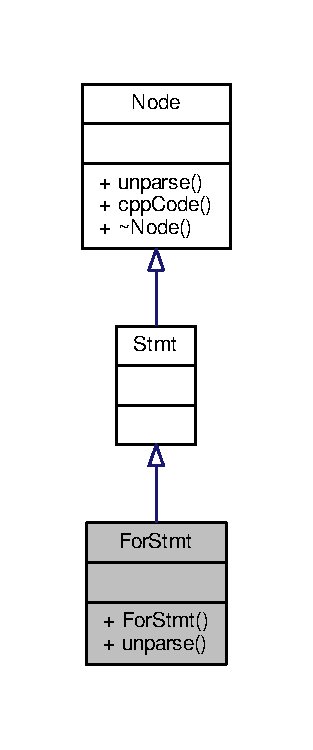
\includegraphics[width=150pt]{classForStmt__inherit__graph}
\end{center}
\end{figure}


Collaboration diagram for For\-Stmt\-:\nopagebreak
\begin{figure}[H]
\begin{center}
\leavevmode
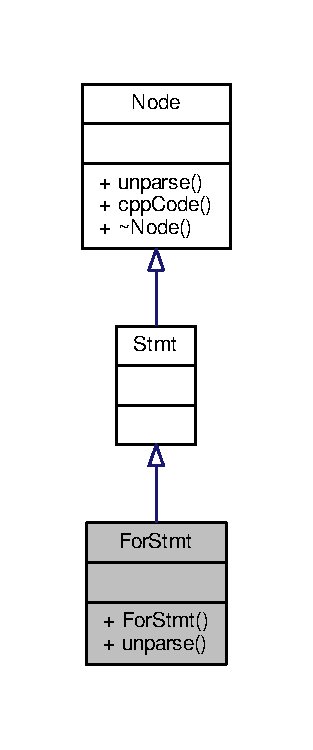
\includegraphics[width=150pt]{classForStmt__coll__graph}
\end{center}
\end{figure}
\subsection*{Public Member Functions}
\begin{DoxyCompactItemize}
\item 
\hyperlink{classForStmt_a2ae00de4dde21c01dab79fa9f53ea747}{For\-Stmt} (\hyperlink{classVarName}{Var\-Name} $\ast$v, \hyperlink{classExpr}{Expr} $\ast$e1, \hyperlink{classExpr}{Expr} $\ast$e2, \hyperlink{classStmt}{Stmt} $\ast$s)
\item 
std\-::string \hyperlink{classForStmt_a9cf08250042ae5a0a54d2196b584e28e}{unparse} ()
\begin{DoxyCompactList}\small\item\em Returns a string representation of the code modeled by this class and all its variables. \end{DoxyCompactList}\end{DoxyCompactItemize}


\subsection{Detailed Description}
Represents a for-\/loop statement. \par
 

Model\-: \hyperlink{classStmt}{Stmt} \-:\-:= 'for' '(' var\-Name '=' \hyperlink{classExpr}{Expr} '\-:' \hyperlink{classExpr}{Expr} ')' \hyperlink{classStmt}{Stmt} \par
 Example\-: for (i = 1\-: 10) \{ print(i); \} 

\subsection{Constructor \& Destructor Documentation}
\hypertarget{classForStmt_a2ae00de4dde21c01dab79fa9f53ea747}{\index{For\-Stmt@{For\-Stmt}!For\-Stmt@{For\-Stmt}}
\index{For\-Stmt@{For\-Stmt}!ForStmt@{For\-Stmt}}
\subsubsection[{For\-Stmt}]{\setlength{\rightskip}{0pt plus 5cm}For\-Stmt\-::\-For\-Stmt (
\begin{DoxyParamCaption}
\item[{{\bf Var\-Name} $\ast$}]{v, }
\item[{{\bf Expr} $\ast$}]{e1, }
\item[{{\bf Expr} $\ast$}]{e2, }
\item[{{\bf Stmt} $\ast$}]{s}
\end{DoxyParamCaption}
)\hspace{0.3cm}{\ttfamily [inline]}}}\label{classForStmt_a2ae00de4dde21c01dab79fa9f53ea747}
Public constructor. 
\begin{DoxyParams}{Parameters}
{\em v} & -\/ Variable that will change each time through the loop \\
\hline
{\em e1} & -\/ Original value given to the variable on first iteration \\
\hline
{\em e2} & -\/ Expression of the stopping value of the variable through the iteration \\
\hline
{\em s} & -\/ Expression to be executed for each iteration \\
\hline
\end{DoxyParams}


\subsection{Member Function Documentation}
\hypertarget{classForStmt_a9cf08250042ae5a0a54d2196b584e28e}{\index{For\-Stmt@{For\-Stmt}!unparse@{unparse}}
\index{unparse@{unparse}!ForStmt@{For\-Stmt}}
\subsubsection[{unparse}]{\setlength{\rightskip}{0pt plus 5cm}string For\-Stmt\-::unparse (
\begin{DoxyParamCaption}
{}
\end{DoxyParamCaption}
)\hspace{0.3cm}{\ttfamily [virtual]}}}\label{classForStmt_a9cf08250042ae5a0a54d2196b584e28e}


Returns a string representation of the code modeled by this class and all its variables. 

\begin{DoxyReturn}{Returns}
std\-::string. 
\end{DoxyReturn}


Implements \hyperlink{classNode_a60ea533e0900961c05e701db70097136}{Node}.



The documentation for this class was generated from the following files\-:\begin{DoxyCompactItemize}
\item 
\hyperlink{AST_8h}{A\-S\-T.\-h}\item 
\hyperlink{AST_8cpp}{A\-S\-T.\-cpp}\end{DoxyCompactItemize}

\hypertarget{classForwardSlashToken}{\section{Forward\-Slash\-Token Class Reference}
\label{classForwardSlashToken}\index{Forward\-Slash\-Token@{Forward\-Slash\-Token}}
}


{\ttfamily \#include $<$ext\-Token.\-h$>$}



Inheritance diagram for Forward\-Slash\-Token\-:\nopagebreak
\begin{figure}[H]
\begin{center}
\leavevmode
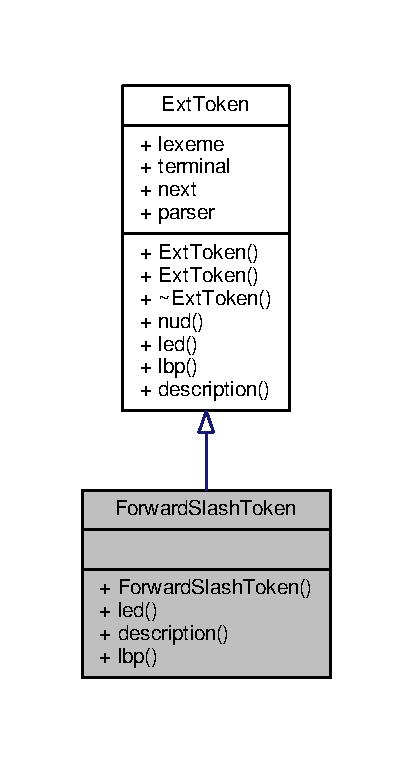
\includegraphics[width=198pt]{classForwardSlashToken__inherit__graph}
\end{center}
\end{figure}


Collaboration diagram for Forward\-Slash\-Token\-:\nopagebreak
\begin{figure}[H]
\begin{center}
\leavevmode
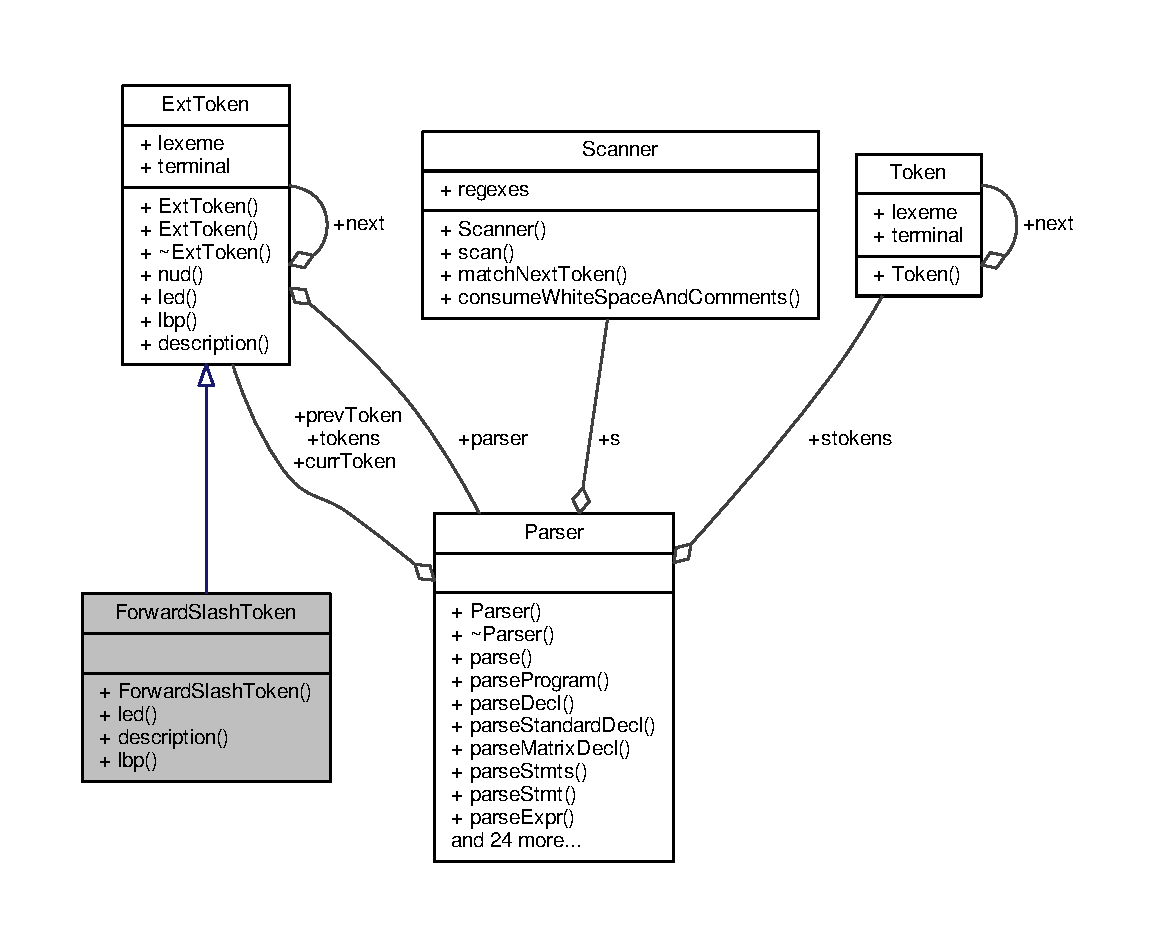
\includegraphics[width=350pt]{classForwardSlashToken__coll__graph}
\end{center}
\end{figure}
\subsection*{Public Member Functions}
\begin{DoxyCompactItemize}
\item 
\hyperlink{classForwardSlashToken_ae818840269cd15f6f6b00929fb4eb979}{Forward\-Slash\-Token} (\hyperlink{classParser}{Parser} $\ast$p, \hyperlink{classToken}{Token} $\ast$t)
\item 
\hyperlink{classParseResult}{Parse\-Result} \hyperlink{classForwardSlashToken_ac2dda7b791ab555e4323f17baaf323e1}{led} (\hyperlink{classParseResult}{Parse\-Result} left)
\item 
std\-::string \hyperlink{classForwardSlashToken_ac27b1ab175ec08c468bd0d4c41636a5c}{description} ()
\item 
int \hyperlink{classForwardSlashToken_ad65829044355922a291dfbfd3052b183}{lbp} ()
\end{DoxyCompactItemize}
\subsection*{Additional Inherited Members}


\subsection{Constructor \& Destructor Documentation}
\hypertarget{classForwardSlashToken_ae818840269cd15f6f6b00929fb4eb979}{\index{Forward\-Slash\-Token@{Forward\-Slash\-Token}!Forward\-Slash\-Token@{Forward\-Slash\-Token}}
\index{Forward\-Slash\-Token@{Forward\-Slash\-Token}!ForwardSlashToken@{Forward\-Slash\-Token}}
\subsubsection[{Forward\-Slash\-Token}]{\setlength{\rightskip}{0pt plus 5cm}Forward\-Slash\-Token\-::\-Forward\-Slash\-Token (
\begin{DoxyParamCaption}
\item[{{\bf Parser} $\ast$}]{p, }
\item[{{\bf Token} $\ast$}]{t}
\end{DoxyParamCaption}
)\hspace{0.3cm}{\ttfamily [inline]}}}\label{classForwardSlashToken_ae818840269cd15f6f6b00929fb4eb979}


\subsection{Member Function Documentation}
\hypertarget{classForwardSlashToken_ac27b1ab175ec08c468bd0d4c41636a5c}{\index{Forward\-Slash\-Token@{Forward\-Slash\-Token}!description@{description}}
\index{description@{description}!ForwardSlashToken@{Forward\-Slash\-Token}}
\subsubsection[{description}]{\setlength{\rightskip}{0pt plus 5cm}std\-::string Forward\-Slash\-Token\-::description (
\begin{DoxyParamCaption}
{}
\end{DoxyParamCaption}
)\hspace{0.3cm}{\ttfamily [inline]}, {\ttfamily [virtual]}}}\label{classForwardSlashToken_ac27b1ab175ec08c468bd0d4c41636a5c}


Reimplemented from \hyperlink{classExtToken_a4ab6e72ac23235650b1756f794172ebb}{Ext\-Token}.

\hypertarget{classForwardSlashToken_ad65829044355922a291dfbfd3052b183}{\index{Forward\-Slash\-Token@{Forward\-Slash\-Token}!lbp@{lbp}}
\index{lbp@{lbp}!ForwardSlashToken@{Forward\-Slash\-Token}}
\subsubsection[{lbp}]{\setlength{\rightskip}{0pt plus 5cm}int Forward\-Slash\-Token\-::lbp (
\begin{DoxyParamCaption}
{}
\end{DoxyParamCaption}
)\hspace{0.3cm}{\ttfamily [inline]}, {\ttfamily [virtual]}}}\label{classForwardSlashToken_ad65829044355922a291dfbfd3052b183}


Reimplemented from \hyperlink{classExtToken_a6c0d61faa058b71147dd54bacee1db94}{Ext\-Token}.

\hypertarget{classForwardSlashToken_ac2dda7b791ab555e4323f17baaf323e1}{\index{Forward\-Slash\-Token@{Forward\-Slash\-Token}!led@{led}}
\index{led@{led}!ForwardSlashToken@{Forward\-Slash\-Token}}
\subsubsection[{led}]{\setlength{\rightskip}{0pt plus 5cm}{\bf Parse\-Result} Forward\-Slash\-Token\-::led (
\begin{DoxyParamCaption}
\item[{{\bf Parse\-Result}}]{left}
\end{DoxyParamCaption}
)\hspace{0.3cm}{\ttfamily [inline]}, {\ttfamily [virtual]}}}\label{classForwardSlashToken_ac2dda7b791ab555e4323f17baaf323e1}


Reimplemented from \hyperlink{classExtToken_afb2c9b0040e198d1d8aa2e041c5a7211}{Ext\-Token}.



The documentation for this class was generated from the following file\-:\begin{DoxyCompactItemize}
\item 
\hyperlink{extToken_8h}{ext\-Token.\-h}\end{DoxyCompactItemize}

\hypertarget{classFunctionCall}{\section{Function\-Call Class Reference}
\label{classFunctionCall}\index{Function\-Call@{Function\-Call}}
}


Represents a function call. \par
  




{\ttfamily \#include $<$A\-S\-T.\-h$>$}



Inheritance diagram for Function\-Call\-:\nopagebreak
\begin{figure}[H]
\begin{center}
\leavevmode
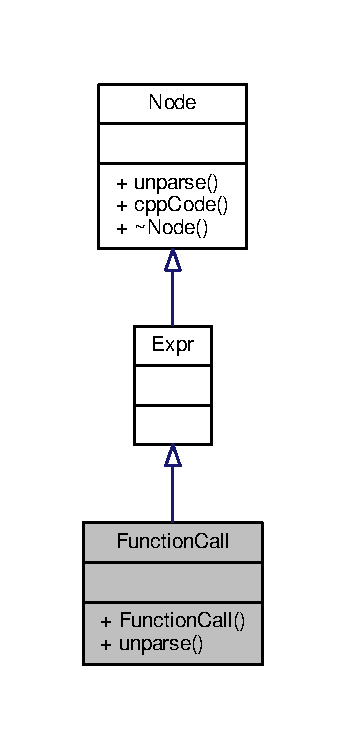
\includegraphics[width=166pt]{classFunctionCall__inherit__graph}
\end{center}
\end{figure}


Collaboration diagram for Function\-Call\-:\nopagebreak
\begin{figure}[H]
\begin{center}
\leavevmode
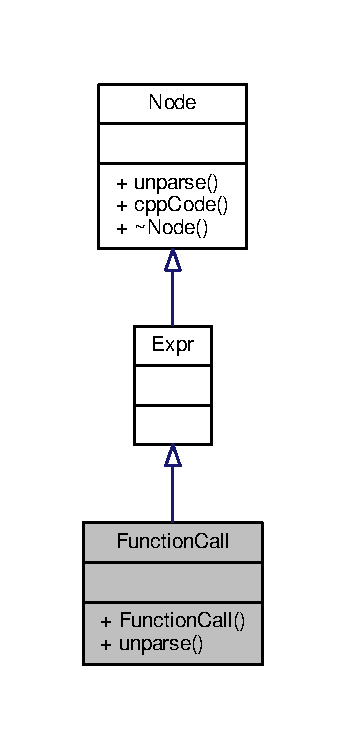
\includegraphics[width=166pt]{classFunctionCall__coll__graph}
\end{center}
\end{figure}
\subsection*{Public Member Functions}
\begin{DoxyCompactItemize}
\item 
\hyperlink{classFunctionCall_ac233a4d5357e0eeb59ff8a0b9d075d28}{Function\-Call} (\hyperlink{classVarName}{Var\-Name} $\ast$v, \hyperlink{classExpr}{Expr} $\ast$e)
\item 
std\-::string \hyperlink{classFunctionCall_aa80e938636e993ed9956e11a51858b95}{unparse} ()
\begin{DoxyCompactList}\small\item\em Returns a string representation of the code modeled by this class and all its variables. \end{DoxyCompactList}\end{DoxyCompactItemize}


\subsection{Detailed Description}
Represents a function call. \par
 

Model\-: \hyperlink{classExpr}{Expr} \-:\-:= var\-Name '(' \hyperlink{classExpr}{Expr} ')' \par
 Example\-: main(1) 

\subsection{Constructor \& Destructor Documentation}
\hypertarget{classFunctionCall_ac233a4d5357e0eeb59ff8a0b9d075d28}{\index{Function\-Call@{Function\-Call}!Function\-Call@{Function\-Call}}
\index{Function\-Call@{Function\-Call}!FunctionCall@{Function\-Call}}
\subsubsection[{Function\-Call}]{\setlength{\rightskip}{0pt plus 5cm}Function\-Call\-::\-Function\-Call (
\begin{DoxyParamCaption}
\item[{{\bf Var\-Name} $\ast$}]{v, }
\item[{{\bf Expr} $\ast$}]{e}
\end{DoxyParamCaption}
)\hspace{0.3cm}{\ttfamily [inline]}}}\label{classFunctionCall_ac233a4d5357e0eeb59ff8a0b9d075d28}
Public constructor. 
\begin{DoxyParams}{Parameters}
{\em v} & -\/ Name of function being called \\
\hline
{\em e} & -\/ Expression of arguments \\
\hline
\end{DoxyParams}


\subsection{Member Function Documentation}
\hypertarget{classFunctionCall_aa80e938636e993ed9956e11a51858b95}{\index{Function\-Call@{Function\-Call}!unparse@{unparse}}
\index{unparse@{unparse}!FunctionCall@{Function\-Call}}
\subsubsection[{unparse}]{\setlength{\rightskip}{0pt plus 5cm}string Function\-Call\-::unparse (
\begin{DoxyParamCaption}
{}
\end{DoxyParamCaption}
)\hspace{0.3cm}{\ttfamily [virtual]}}}\label{classFunctionCall_aa80e938636e993ed9956e11a51858b95}


Returns a string representation of the code modeled by this class and all its variables. 

\begin{DoxyReturn}{Returns}
std\-::string. 
\end{DoxyReturn}


Implements \hyperlink{classNode_a60ea533e0900961c05e701db70097136}{Node}.



The documentation for this class was generated from the following files\-:\begin{DoxyCompactItemize}
\item 
\hyperlink{AST_8h}{A\-S\-T.\-h}\item 
\hyperlink{AST_8cpp}{A\-S\-T.\-cpp}\end{DoxyCompactItemize}

\hypertarget{classIfElseStmt}{\section{If\-Else\-Stmt Class Reference}
\label{classIfElseStmt}\index{If\-Else\-Stmt@{If\-Else\-Stmt}}
}


Represents an if-\/else statement. \par
  




{\ttfamily \#include $<$A\-S\-T.\-h$>$}



Inheritance diagram for If\-Else\-Stmt\-:\nopagebreak
\begin{figure}[H]
\begin{center}
\leavevmode
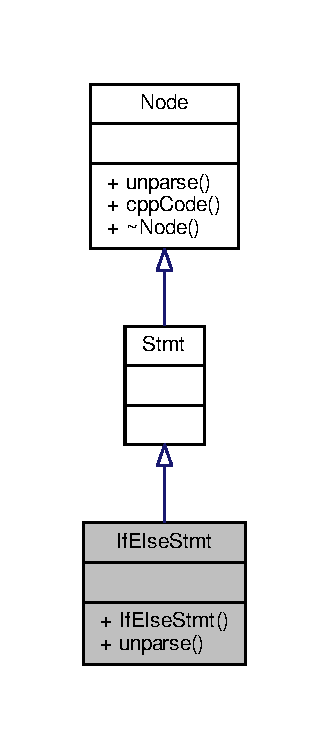
\includegraphics[width=158pt]{classIfElseStmt__inherit__graph}
\end{center}
\end{figure}


Collaboration diagram for If\-Else\-Stmt\-:\nopagebreak
\begin{figure}[H]
\begin{center}
\leavevmode
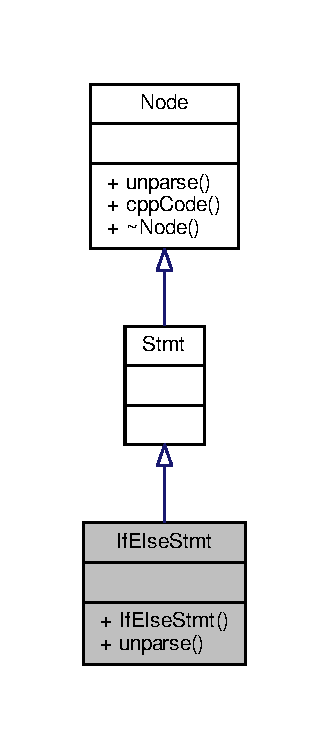
\includegraphics[width=158pt]{classIfElseStmt__coll__graph}
\end{center}
\end{figure}
\subsection*{Public Member Functions}
\begin{DoxyCompactItemize}
\item 
\hyperlink{classIfElseStmt_a9e0fde33a0889aa64175dfdf7e7326da}{If\-Else\-Stmt} (\hyperlink{classExpr}{Expr} $\ast$e, \hyperlink{classStmt}{Stmt} $\ast$s1, \hyperlink{classStmt}{Stmt} $\ast$s2)
\item 
std\-::string \hyperlink{classIfElseStmt_a2e8c850644f33e4ba918c53d0212e59f}{unparse} ()
\begin{DoxyCompactList}\small\item\em Returns a string representation of the code modeled by this class and all its variables. \end{DoxyCompactList}\end{DoxyCompactItemize}


\subsection{Detailed Description}
Represents an if-\/else statement. \par
 

Model\-: \hyperlink{classStmt}{Stmt} \-:\-:= 'if' '(' \hyperlink{classExpr}{Expr} ')' \hyperlink{classStmt}{Stmt} 'else' \hyperlink{classStmt}{Stmt} \par
 Example\-: if (True) \{ x += 1; \} else \{ x -\/= 1; \} 

\subsection{Constructor \& Destructor Documentation}
\hypertarget{classIfElseStmt_a9e0fde33a0889aa64175dfdf7e7326da}{\index{If\-Else\-Stmt@{If\-Else\-Stmt}!If\-Else\-Stmt@{If\-Else\-Stmt}}
\index{If\-Else\-Stmt@{If\-Else\-Stmt}!IfElseStmt@{If\-Else\-Stmt}}
\subsubsection[{If\-Else\-Stmt}]{\setlength{\rightskip}{0pt plus 5cm}If\-Else\-Stmt\-::\-If\-Else\-Stmt (
\begin{DoxyParamCaption}
\item[{{\bf Expr} $\ast$}]{e, }
\item[{{\bf Stmt} $\ast$}]{s1, }
\item[{{\bf Stmt} $\ast$}]{s2}
\end{DoxyParamCaption}
)\hspace{0.3cm}{\ttfamily [inline]}}}\label{classIfElseStmt_a9e0fde33a0889aa64175dfdf7e7326da}
Public constructor. 
\begin{DoxyParams}{Parameters}
{\em e} & -\/ Boolean expression that is evaluated by if \\
\hline
{\em s1} & -\/ Statement to be executed if true \\
\hline
{\em s2} & -\/ Statement to be executed if false \\
\hline
\end{DoxyParams}


\subsection{Member Function Documentation}
\hypertarget{classIfElseStmt_a2e8c850644f33e4ba918c53d0212e59f}{\index{If\-Else\-Stmt@{If\-Else\-Stmt}!unparse@{unparse}}
\index{unparse@{unparse}!IfElseStmt@{If\-Else\-Stmt}}
\subsubsection[{unparse}]{\setlength{\rightskip}{0pt plus 5cm}string If\-Else\-Stmt\-::unparse (
\begin{DoxyParamCaption}
{}
\end{DoxyParamCaption}
)\hspace{0.3cm}{\ttfamily [virtual]}}}\label{classIfElseStmt_a2e8c850644f33e4ba918c53d0212e59f}


Returns a string representation of the code modeled by this class and all its variables. 

\begin{DoxyReturn}{Returns}
std\-::string. 
\end{DoxyReturn}


Implements \hyperlink{classNode_a60ea533e0900961c05e701db70097136}{Node}.



The documentation for this class was generated from the following files\-:\begin{DoxyCompactItemize}
\item 
\hyperlink{AST_8h}{A\-S\-T.\-h}\item 
\hyperlink{AST_8cpp}{A\-S\-T.\-cpp}\end{DoxyCompactItemize}

\hypertarget{classIfExpr}{\section{If\-Expr Class Reference}
\label{classIfExpr}\index{If\-Expr@{If\-Expr}}
}


Represents if-\/then-\/else expression \par
  




{\ttfamily \#include $<$A\-S\-T.\-h$>$}



Inheritance diagram for If\-Expr\-:\nopagebreak
\begin{figure}[H]
\begin{center}
\leavevmode
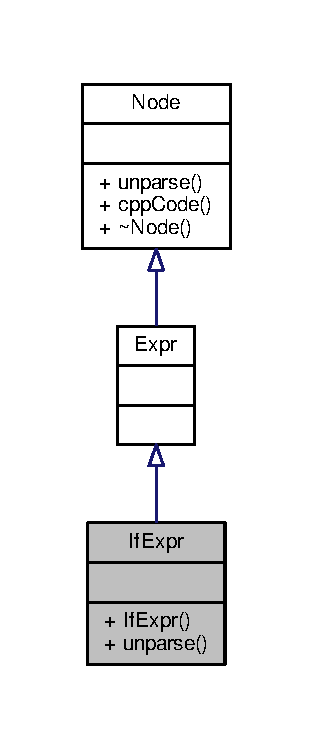
\includegraphics[width=150pt]{classIfExpr__inherit__graph}
\end{center}
\end{figure}


Collaboration diagram for If\-Expr\-:\nopagebreak
\begin{figure}[H]
\begin{center}
\leavevmode
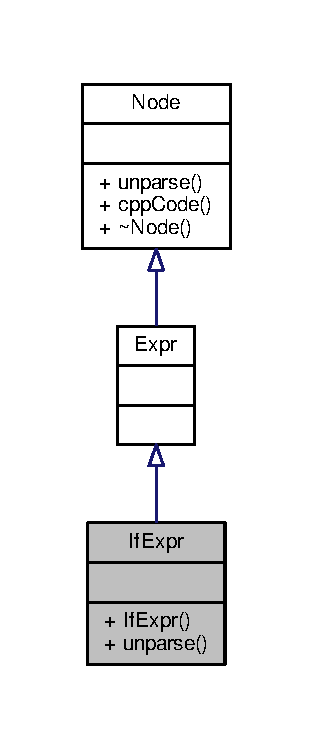
\includegraphics[width=150pt]{classIfExpr__coll__graph}
\end{center}
\end{figure}
\subsection*{Public Member Functions}
\begin{DoxyCompactItemize}
\item 
\hyperlink{classIfExpr_a8ade872da7dc8d8d80c6d5897353e0ae}{If\-Expr} (\hyperlink{classExpr}{Expr} $\ast$e1, \hyperlink{classExpr}{Expr} $\ast$e2, \hyperlink{classExpr}{Expr} $\ast$e3)
\item 
std\-::string \hyperlink{classIfExpr_a4b4c34fffb9539bac51cf5eb35e30081}{unparse} ()
\begin{DoxyCompactList}\small\item\em Returns a string representation of the code modeled by this class and all its variables. \end{DoxyCompactList}\end{DoxyCompactItemize}


\subsection{Detailed Description}
Represents if-\/then-\/else expression \par
 

Model\-: \hyperlink{classExpr}{Expr} \-:\-:= 'if' \hyperlink{classExpr}{Expr} 'then' \hyperlink{classExpr}{Expr} 'else' \hyperlink{classExpr}{Expr} \par
 Example\-: if True then print(\char`\"{}\-Hello World\char`\"{}); else print(\char`\"{}\-This will never be read!!!\char`\"{}); 

\subsection{Constructor \& Destructor Documentation}
\hypertarget{classIfExpr_a8ade872da7dc8d8d80c6d5897353e0ae}{\index{If\-Expr@{If\-Expr}!If\-Expr@{If\-Expr}}
\index{If\-Expr@{If\-Expr}!IfExpr@{If\-Expr}}
\subsubsection[{If\-Expr}]{\setlength{\rightskip}{0pt plus 5cm}If\-Expr\-::\-If\-Expr (
\begin{DoxyParamCaption}
\item[{{\bf Expr} $\ast$}]{e1, }
\item[{{\bf Expr} $\ast$}]{e2, }
\item[{{\bf Expr} $\ast$}]{e3}
\end{DoxyParamCaption}
)\hspace{0.3cm}{\ttfamily [inline]}}}\label{classIfExpr_a8ade872da7dc8d8d80c6d5897353e0ae}
Public constructor. 
\begin{DoxyParams}{Parameters}
{\em e1} & -\/ Boolean expression to be considered \\
\hline
{\em e2} & -\/ Expression to be evaluated if true \\
\hline
{\em e3} & -\/ Expression to be evaluated if false \\
\hline
\end{DoxyParams}


\subsection{Member Function Documentation}
\hypertarget{classIfExpr_a4b4c34fffb9539bac51cf5eb35e30081}{\index{If\-Expr@{If\-Expr}!unparse@{unparse}}
\index{unparse@{unparse}!IfExpr@{If\-Expr}}
\subsubsection[{unparse}]{\setlength{\rightskip}{0pt plus 5cm}string If\-Expr\-::unparse (
\begin{DoxyParamCaption}
{}
\end{DoxyParamCaption}
)\hspace{0.3cm}{\ttfamily [virtual]}}}\label{classIfExpr_a4b4c34fffb9539bac51cf5eb35e30081}


Returns a string representation of the code modeled by this class and all its variables. 

\begin{DoxyReturn}{Returns}
std\-::string. 
\end{DoxyReturn}


Implements \hyperlink{classNode_a60ea533e0900961c05e701db70097136}{Node}.



The documentation for this class was generated from the following files\-:\begin{DoxyCompactItemize}
\item 
\hyperlink{AST_8h}{A\-S\-T.\-h}\item 
\hyperlink{AST_8cpp}{A\-S\-T.\-cpp}\end{DoxyCompactItemize}

\hypertarget{classIfStmt}{\section{If\-Stmt Class Reference}
\label{classIfStmt}\index{If\-Stmt@{If\-Stmt}}
}


Represents an if statement. \par
  




{\ttfamily \#include $<$A\-S\-T.\-h$>$}



Inheritance diagram for If\-Stmt\-:\nopagebreak
\begin{figure}[H]
\begin{center}
\leavevmode
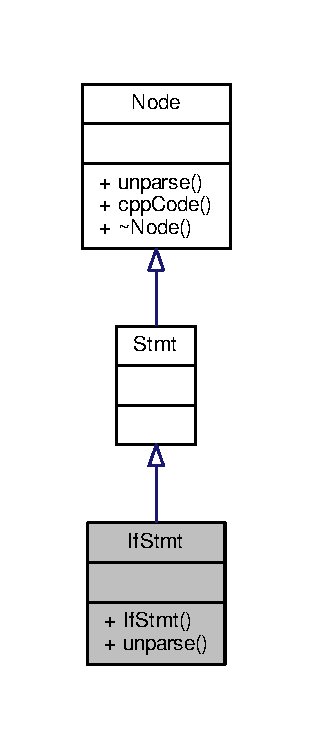
\includegraphics[width=150pt]{classIfStmt__inherit__graph}
\end{center}
\end{figure}


Collaboration diagram for If\-Stmt\-:\nopagebreak
\begin{figure}[H]
\begin{center}
\leavevmode
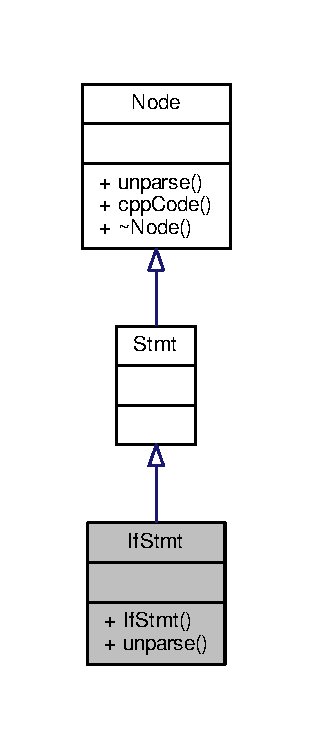
\includegraphics[width=150pt]{classIfStmt__coll__graph}
\end{center}
\end{figure}
\subsection*{Public Member Functions}
\begin{DoxyCompactItemize}
\item 
\hyperlink{classIfStmt_a917206365fb4307ede6751d2d00e0a58}{If\-Stmt} (\hyperlink{classExpr}{Expr} $\ast$e, \hyperlink{classStmt}{Stmt} $\ast$s)
\item 
std\-::string \hyperlink{classIfStmt_abc1ada72841299826de65fbdf5dc36a0}{unparse} ()
\begin{DoxyCompactList}\small\item\em Returns a string representation of the code modeled by this class and all its variables. \end{DoxyCompactList}\end{DoxyCompactItemize}


\subsection{Detailed Description}
Represents an if statement. \par
 

Model\-: \hyperlink{classStmt}{Stmt} \-:\-:= 'if' '(' \hyperlink{classExpr}{Expr} ')' \hyperlink{classStmt}{Stmt} \par
 Example\-: if (True) \{ x += 1; \} 

\subsection{Constructor \& Destructor Documentation}
\hypertarget{classIfStmt_a917206365fb4307ede6751d2d00e0a58}{\index{If\-Stmt@{If\-Stmt}!If\-Stmt@{If\-Stmt}}
\index{If\-Stmt@{If\-Stmt}!IfStmt@{If\-Stmt}}
\subsubsection[{If\-Stmt}]{\setlength{\rightskip}{0pt plus 5cm}If\-Stmt\-::\-If\-Stmt (
\begin{DoxyParamCaption}
\item[{{\bf Expr} $\ast$}]{e, }
\item[{{\bf Stmt} $\ast$}]{s}
\end{DoxyParamCaption}
)\hspace{0.3cm}{\ttfamily [inline]}}}\label{classIfStmt_a917206365fb4307ede6751d2d00e0a58}
Public constructor. 
\begin{DoxyParams}{Parameters}
{\em e} & -\/ Boolean expression that is evaluated by if \\
\hline
{\em s} & -\/ Statement to be executed if true \\
\hline
\end{DoxyParams}


\subsection{Member Function Documentation}
\hypertarget{classIfStmt_abc1ada72841299826de65fbdf5dc36a0}{\index{If\-Stmt@{If\-Stmt}!unparse@{unparse}}
\index{unparse@{unparse}!IfStmt@{If\-Stmt}}
\subsubsection[{unparse}]{\setlength{\rightskip}{0pt plus 5cm}string If\-Stmt\-::unparse (
\begin{DoxyParamCaption}
{}
\end{DoxyParamCaption}
)\hspace{0.3cm}{\ttfamily [virtual]}}}\label{classIfStmt_abc1ada72841299826de65fbdf5dc36a0}


Returns a string representation of the code modeled by this class and all its variables. 

\begin{DoxyReturn}{Returns}
std\-::string. 
\end{DoxyReturn}


Implements \hyperlink{classNode_a60ea533e0900961c05e701db70097136}{Node}.



The documentation for this class was generated from the following files\-:\begin{DoxyCompactItemize}
\item 
\hyperlink{AST_8h}{A\-S\-T.\-h}\item 
\hyperlink{AST_8cpp}{A\-S\-T.\-cpp}\end{DoxyCompactItemize}

\hypertarget{classIfToken}{\section{If\-Token Class Reference}
\label{classIfToken}\index{If\-Token@{If\-Token}}
}


{\ttfamily \#include $<$ext\-Token.\-h$>$}



Inheritance diagram for If\-Token\-:\nopagebreak
\begin{figure}[H]
\begin{center}
\leavevmode
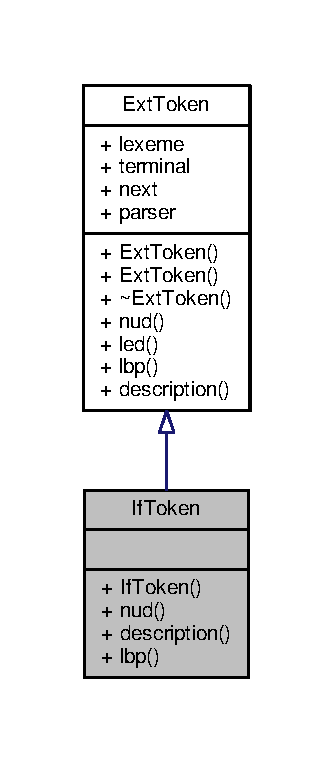
\includegraphics[width=160pt]{classIfToken__inherit__graph}
\end{center}
\end{figure}


Collaboration diagram for If\-Token\-:\nopagebreak
\begin{figure}[H]
\begin{center}
\leavevmode
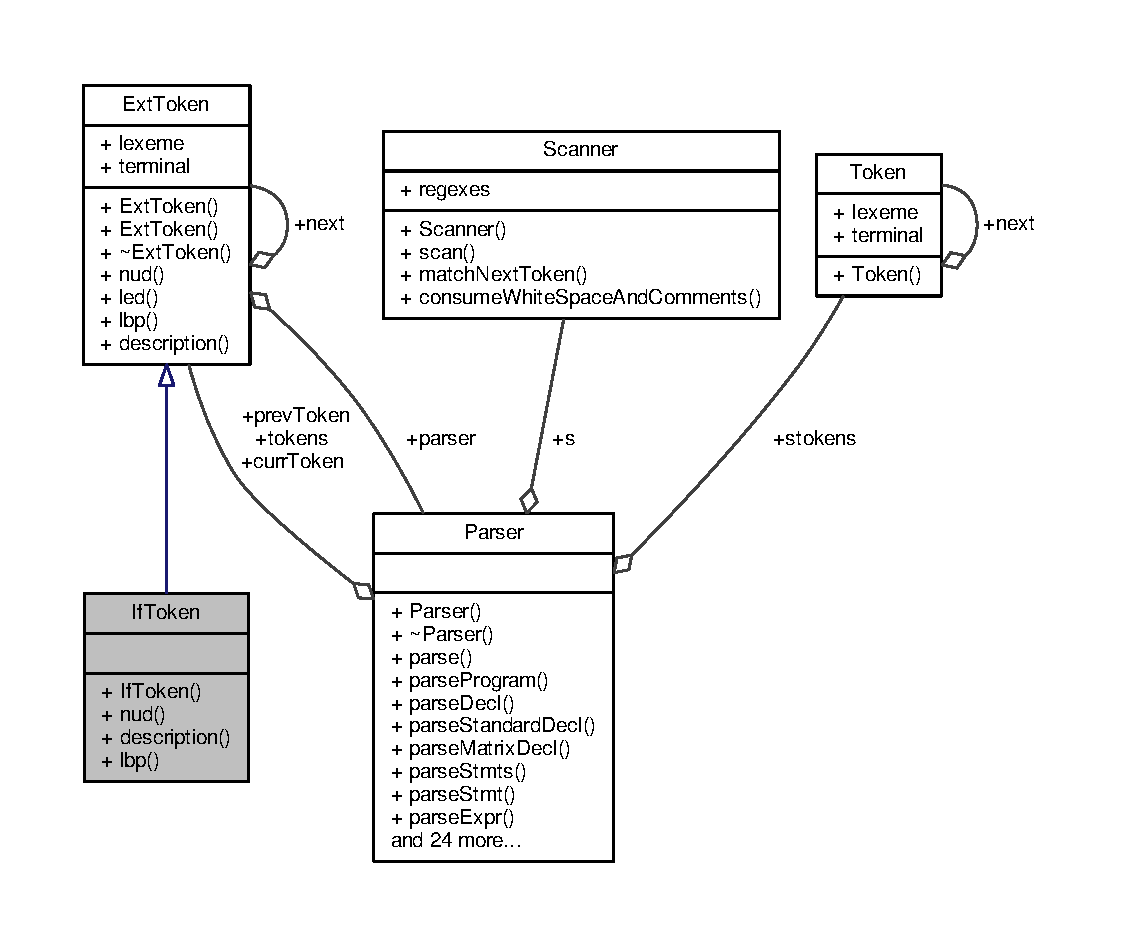
\includegraphics[width=350pt]{classIfToken__coll__graph}
\end{center}
\end{figure}
\subsection*{Public Member Functions}
\begin{DoxyCompactItemize}
\item 
\hyperlink{classIfToken_a607028595b06b8a950000ba3e82329db}{If\-Token} (\hyperlink{classParser}{Parser} $\ast$p, \hyperlink{classToken}{Token} $\ast$t)
\item 
\hyperlink{classParseResult}{Parse\-Result} \hyperlink{classIfToken_add06bd79ce755fd5503f78e507109e52}{nud} ()
\item 
std\-::string \hyperlink{classIfToken_aad226162c5649920c13c2a9e9e7a3617}{description} ()
\item 
int \hyperlink{classIfToken_abfd39ff4c4818d382bf0b97fd097c478}{lbp} ()
\end{DoxyCompactItemize}
\subsection*{Additional Inherited Members}


\subsection{Constructor \& Destructor Documentation}
\hypertarget{classIfToken_a607028595b06b8a950000ba3e82329db}{\index{If\-Token@{If\-Token}!If\-Token@{If\-Token}}
\index{If\-Token@{If\-Token}!IfToken@{If\-Token}}
\subsubsection[{If\-Token}]{\setlength{\rightskip}{0pt plus 5cm}If\-Token\-::\-If\-Token (
\begin{DoxyParamCaption}
\item[{{\bf Parser} $\ast$}]{p, }
\item[{{\bf Token} $\ast$}]{t}
\end{DoxyParamCaption}
)\hspace{0.3cm}{\ttfamily [inline]}}}\label{classIfToken_a607028595b06b8a950000ba3e82329db}


\subsection{Member Function Documentation}
\hypertarget{classIfToken_aad226162c5649920c13c2a9e9e7a3617}{\index{If\-Token@{If\-Token}!description@{description}}
\index{description@{description}!IfToken@{If\-Token}}
\subsubsection[{description}]{\setlength{\rightskip}{0pt plus 5cm}std\-::string If\-Token\-::description (
\begin{DoxyParamCaption}
{}
\end{DoxyParamCaption}
)\hspace{0.3cm}{\ttfamily [inline]}, {\ttfamily [virtual]}}}\label{classIfToken_aad226162c5649920c13c2a9e9e7a3617}


Reimplemented from \hyperlink{classExtToken_a4ab6e72ac23235650b1756f794172ebb}{Ext\-Token}.

\hypertarget{classIfToken_abfd39ff4c4818d382bf0b97fd097c478}{\index{If\-Token@{If\-Token}!lbp@{lbp}}
\index{lbp@{lbp}!IfToken@{If\-Token}}
\subsubsection[{lbp}]{\setlength{\rightskip}{0pt plus 5cm}int If\-Token\-::lbp (
\begin{DoxyParamCaption}
{}
\end{DoxyParamCaption}
)\hspace{0.3cm}{\ttfamily [inline]}, {\ttfamily [virtual]}}}\label{classIfToken_abfd39ff4c4818d382bf0b97fd097c478}


Reimplemented from \hyperlink{classExtToken_a6c0d61faa058b71147dd54bacee1db94}{Ext\-Token}.

\hypertarget{classIfToken_add06bd79ce755fd5503f78e507109e52}{\index{If\-Token@{If\-Token}!nud@{nud}}
\index{nud@{nud}!IfToken@{If\-Token}}
\subsubsection[{nud}]{\setlength{\rightskip}{0pt plus 5cm}{\bf Parse\-Result} If\-Token\-::nud (
\begin{DoxyParamCaption}
{}
\end{DoxyParamCaption}
)\hspace{0.3cm}{\ttfamily [inline]}, {\ttfamily [virtual]}}}\label{classIfToken_add06bd79ce755fd5503f78e507109e52}


Reimplemented from \hyperlink{classExtToken_a5c21a5ffe91f212085259126652ab77c}{Ext\-Token}.



The documentation for this class was generated from the following file\-:\begin{DoxyCompactItemize}
\item 
\hyperlink{extToken_8h}{ext\-Token.\-h}\end{DoxyCompactItemize}

\hypertarget{classIntConstToken}{\section{Int\-Const\-Token Class Reference}
\label{classIntConstToken}\index{Int\-Const\-Token@{Int\-Const\-Token}}
}


{\ttfamily \#include $<$ext\-Token.\-h$>$}



Inheritance diagram for Int\-Const\-Token\-:\nopagebreak
\begin{figure}[H]
\begin{center}
\leavevmode
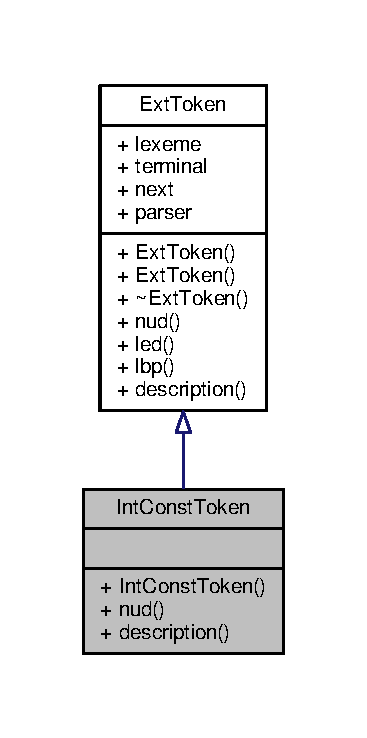
\includegraphics[width=176pt]{classIntConstToken__inherit__graph}
\end{center}
\end{figure}


Collaboration diagram for Int\-Const\-Token\-:\nopagebreak
\begin{figure}[H]
\begin{center}
\leavevmode
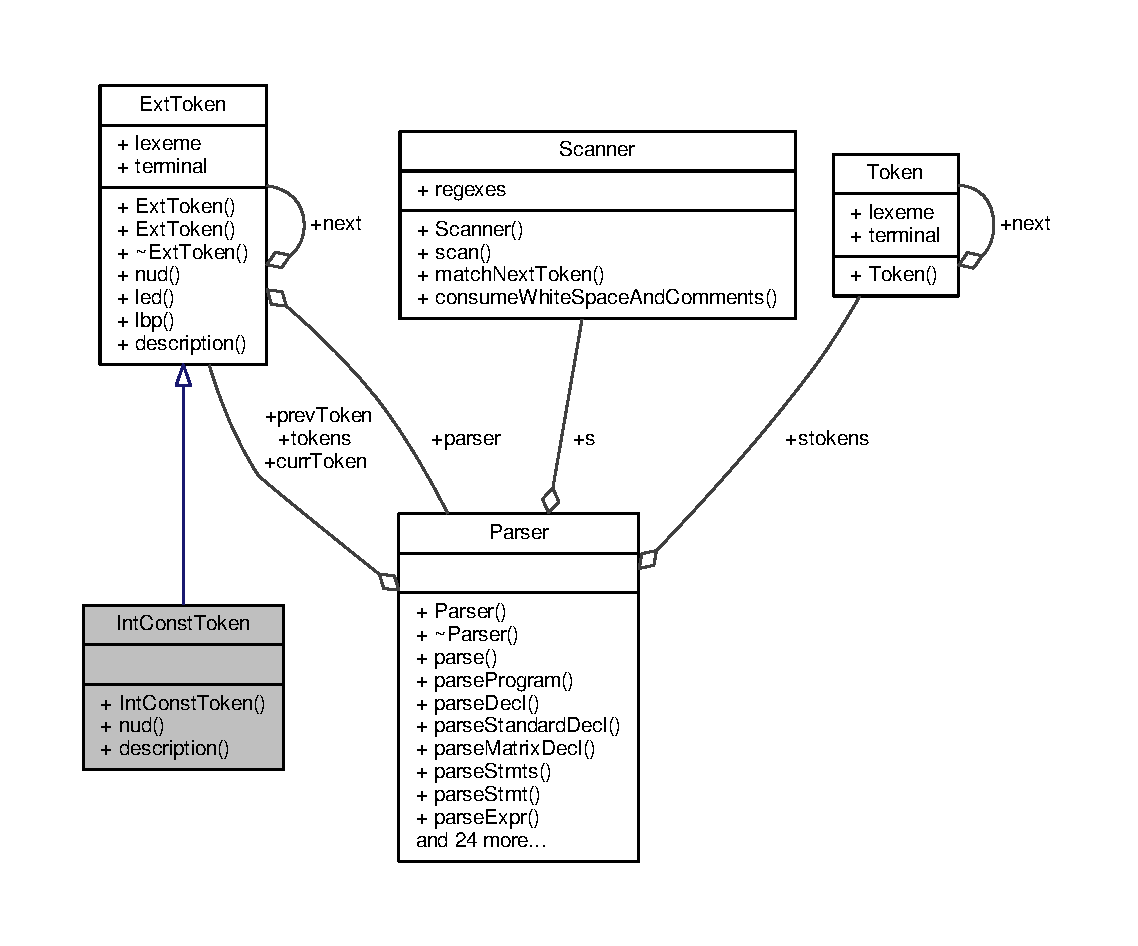
\includegraphics[width=350pt]{classIntConstToken__coll__graph}
\end{center}
\end{figure}
\subsection*{Public Member Functions}
\begin{DoxyCompactItemize}
\item 
\hyperlink{classIntConstToken_a14c6bf0af5a915969b4fef1758067af3}{Int\-Const\-Token} (\hyperlink{classParser}{Parser} $\ast$p, \hyperlink{classToken}{Token} $\ast$t)
\item 
\hyperlink{classParseResult}{Parse\-Result} \hyperlink{classIntConstToken_ae1f720d6006c47e145cae7879d09c708}{nud} ()
\item 
std\-::string \hyperlink{classIntConstToken_a98191508d849878d40800e447a0f1892}{description} ()
\end{DoxyCompactItemize}
\subsection*{Additional Inherited Members}


\subsection{Constructor \& Destructor Documentation}
\hypertarget{classIntConstToken_a14c6bf0af5a915969b4fef1758067af3}{\index{Int\-Const\-Token@{Int\-Const\-Token}!Int\-Const\-Token@{Int\-Const\-Token}}
\index{Int\-Const\-Token@{Int\-Const\-Token}!IntConstToken@{Int\-Const\-Token}}
\subsubsection[{Int\-Const\-Token}]{\setlength{\rightskip}{0pt plus 5cm}Int\-Const\-Token\-::\-Int\-Const\-Token (
\begin{DoxyParamCaption}
\item[{{\bf Parser} $\ast$}]{p, }
\item[{{\bf Token} $\ast$}]{t}
\end{DoxyParamCaption}
)\hspace{0.3cm}{\ttfamily [inline]}}}\label{classIntConstToken_a14c6bf0af5a915969b4fef1758067af3}


\subsection{Member Function Documentation}
\hypertarget{classIntConstToken_a98191508d849878d40800e447a0f1892}{\index{Int\-Const\-Token@{Int\-Const\-Token}!description@{description}}
\index{description@{description}!IntConstToken@{Int\-Const\-Token}}
\subsubsection[{description}]{\setlength{\rightskip}{0pt plus 5cm}std\-::string Int\-Const\-Token\-::description (
\begin{DoxyParamCaption}
{}
\end{DoxyParamCaption}
)\hspace{0.3cm}{\ttfamily [inline]}, {\ttfamily [virtual]}}}\label{classIntConstToken_a98191508d849878d40800e447a0f1892}


Reimplemented from \hyperlink{classExtToken_a4ab6e72ac23235650b1756f794172ebb}{Ext\-Token}.

\hypertarget{classIntConstToken_ae1f720d6006c47e145cae7879d09c708}{\index{Int\-Const\-Token@{Int\-Const\-Token}!nud@{nud}}
\index{nud@{nud}!IntConstToken@{Int\-Const\-Token}}
\subsubsection[{nud}]{\setlength{\rightskip}{0pt plus 5cm}{\bf Parse\-Result} Int\-Const\-Token\-::nud (
\begin{DoxyParamCaption}
{}
\end{DoxyParamCaption}
)\hspace{0.3cm}{\ttfamily [inline]}, {\ttfamily [virtual]}}}\label{classIntConstToken_ae1f720d6006c47e145cae7879d09c708}


Reimplemented from \hyperlink{classExtToken_a5c21a5ffe91f212085259126652ab77c}{Ext\-Token}.



The documentation for this class was generated from the following file\-:\begin{DoxyCompactItemize}
\item 
\hyperlink{extToken_8h}{ext\-Token.\-h}\end{DoxyCompactItemize}

\hypertarget{classLeftParenToken}{\section{Left\-Paren\-Token Class Reference}
\label{classLeftParenToken}\index{Left\-Paren\-Token@{Left\-Paren\-Token}}
}


{\ttfamily \#include $<$ext\-Token.\-h$>$}



Inheritance diagram for Left\-Paren\-Token\-:\nopagebreak
\begin{figure}[H]
\begin{center}
\leavevmode
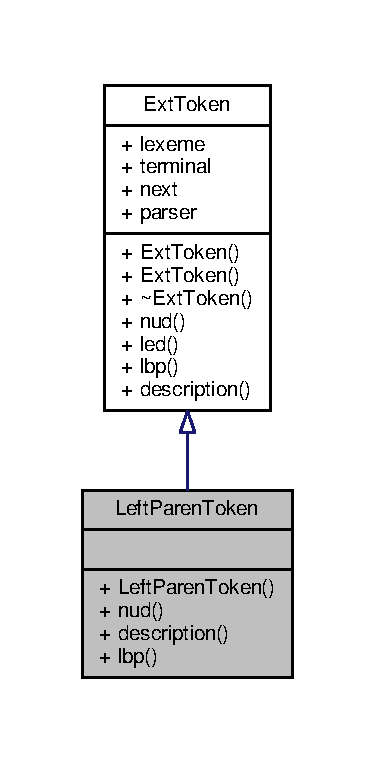
\includegraphics[width=180pt]{classLeftParenToken__inherit__graph}
\end{center}
\end{figure}


Collaboration diagram for Left\-Paren\-Token\-:\nopagebreak
\begin{figure}[H]
\begin{center}
\leavevmode
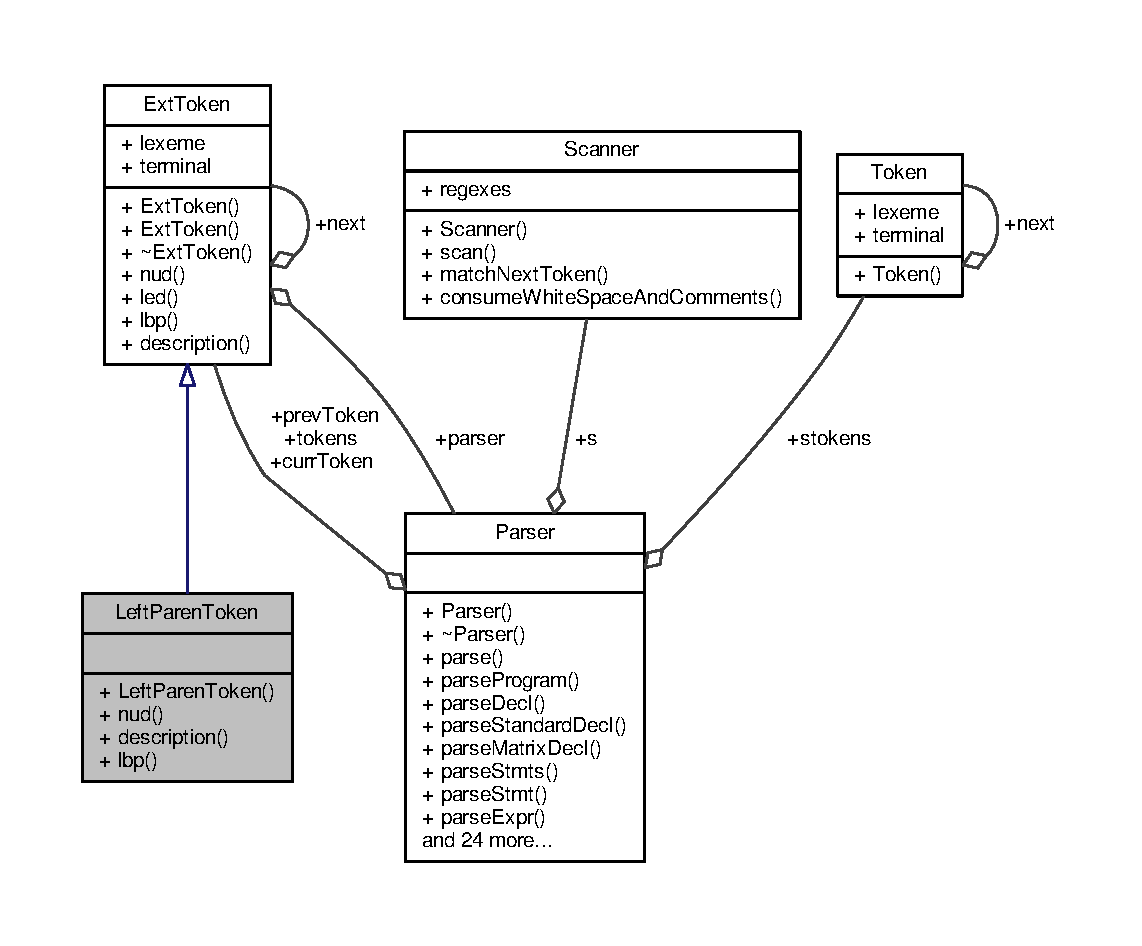
\includegraphics[width=350pt]{classLeftParenToken__coll__graph}
\end{center}
\end{figure}
\subsection*{Public Member Functions}
\begin{DoxyCompactItemize}
\item 
\hyperlink{classLeftParenToken_aecdc6faf48a1a7192ec55712f0264cba}{Left\-Paren\-Token} (\hyperlink{classParser}{Parser} $\ast$p, \hyperlink{classToken}{Token} $\ast$t)
\item 
\hyperlink{classParseResult}{Parse\-Result} \hyperlink{classLeftParenToken_a3cb3ae9ab2647e5534c85529d314f08b}{nud} ()
\item 
std\-::string \hyperlink{classLeftParenToken_a2df35684bd2081c3bdfe2357946917bc}{description} ()
\item 
int \hyperlink{classLeftParenToken_afa1b94645278f097bb097d3b24445d14}{lbp} ()
\end{DoxyCompactItemize}
\subsection*{Additional Inherited Members}


\subsection{Constructor \& Destructor Documentation}
\hypertarget{classLeftParenToken_aecdc6faf48a1a7192ec55712f0264cba}{\index{Left\-Paren\-Token@{Left\-Paren\-Token}!Left\-Paren\-Token@{Left\-Paren\-Token}}
\index{Left\-Paren\-Token@{Left\-Paren\-Token}!LeftParenToken@{Left\-Paren\-Token}}
\subsubsection[{Left\-Paren\-Token}]{\setlength{\rightskip}{0pt plus 5cm}Left\-Paren\-Token\-::\-Left\-Paren\-Token (
\begin{DoxyParamCaption}
\item[{{\bf Parser} $\ast$}]{p, }
\item[{{\bf Token} $\ast$}]{t}
\end{DoxyParamCaption}
)\hspace{0.3cm}{\ttfamily [inline]}}}\label{classLeftParenToken_aecdc6faf48a1a7192ec55712f0264cba}


\subsection{Member Function Documentation}
\hypertarget{classLeftParenToken_a2df35684bd2081c3bdfe2357946917bc}{\index{Left\-Paren\-Token@{Left\-Paren\-Token}!description@{description}}
\index{description@{description}!LeftParenToken@{Left\-Paren\-Token}}
\subsubsection[{description}]{\setlength{\rightskip}{0pt plus 5cm}std\-::string Left\-Paren\-Token\-::description (
\begin{DoxyParamCaption}
{}
\end{DoxyParamCaption}
)\hspace{0.3cm}{\ttfamily [inline]}, {\ttfamily [virtual]}}}\label{classLeftParenToken_a2df35684bd2081c3bdfe2357946917bc}


Reimplemented from \hyperlink{classExtToken_a4ab6e72ac23235650b1756f794172ebb}{Ext\-Token}.

\hypertarget{classLeftParenToken_afa1b94645278f097bb097d3b24445d14}{\index{Left\-Paren\-Token@{Left\-Paren\-Token}!lbp@{lbp}}
\index{lbp@{lbp}!LeftParenToken@{Left\-Paren\-Token}}
\subsubsection[{lbp}]{\setlength{\rightskip}{0pt plus 5cm}int Left\-Paren\-Token\-::lbp (
\begin{DoxyParamCaption}
{}
\end{DoxyParamCaption}
)\hspace{0.3cm}{\ttfamily [inline]}, {\ttfamily [virtual]}}}\label{classLeftParenToken_afa1b94645278f097bb097d3b24445d14}


Reimplemented from \hyperlink{classExtToken_a6c0d61faa058b71147dd54bacee1db94}{Ext\-Token}.

\hypertarget{classLeftParenToken_a3cb3ae9ab2647e5534c85529d314f08b}{\index{Left\-Paren\-Token@{Left\-Paren\-Token}!nud@{nud}}
\index{nud@{nud}!LeftParenToken@{Left\-Paren\-Token}}
\subsubsection[{nud}]{\setlength{\rightskip}{0pt plus 5cm}{\bf Parse\-Result} Left\-Paren\-Token\-::nud (
\begin{DoxyParamCaption}
{}
\end{DoxyParamCaption}
)\hspace{0.3cm}{\ttfamily [inline]}, {\ttfamily [virtual]}}}\label{classLeftParenToken_a3cb3ae9ab2647e5534c85529d314f08b}


Reimplemented from \hyperlink{classExtToken_a5c21a5ffe91f212085259126652ab77c}{Ext\-Token}.



The documentation for this class was generated from the following file\-:\begin{DoxyCompactItemize}
\item 
\hyperlink{extToken_8h}{ext\-Token.\-h}\end{DoxyCompactItemize}

\hypertarget{classLetExpr}{\section{Let\-Expr Class Reference}
\label{classLetExpr}\index{Let\-Expr@{Let\-Expr}}
}


Represents a let expression. \par
  




{\ttfamily \#include $<$A\-S\-T.\-h$>$}



Inheritance diagram for Let\-Expr\-:\nopagebreak
\begin{figure}[H]
\begin{center}
\leavevmode
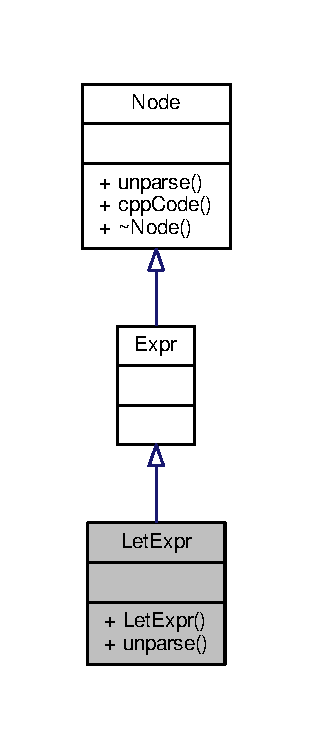
\includegraphics[width=150pt]{classLetExpr__inherit__graph}
\end{center}
\end{figure}


Collaboration diagram for Let\-Expr\-:\nopagebreak
\begin{figure}[H]
\begin{center}
\leavevmode
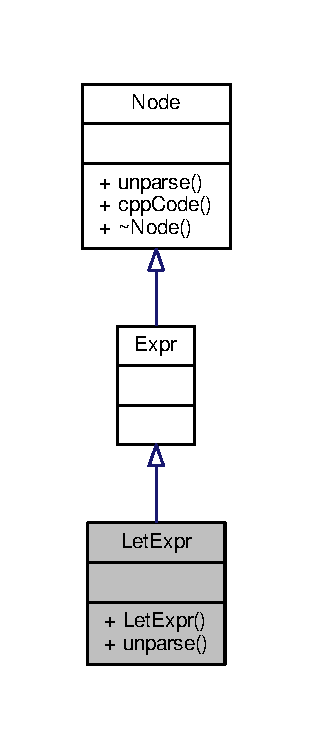
\includegraphics[width=150pt]{classLetExpr__coll__graph}
\end{center}
\end{figure}
\subsection*{Public Member Functions}
\begin{DoxyCompactItemize}
\item 
\hyperlink{classLetExpr_aeed5f20120434ad46cdb0ddca148603b}{Let\-Expr} (\hyperlink{classStmts}{Stmts} $\ast$s, \hyperlink{classExpr}{Expr} $\ast$e)
\item 
std\-::string \hyperlink{classLetExpr_a518a538c87aeec36204d8a465be32913}{unparse} ()
\begin{DoxyCompactList}\small\item\em Returns a string representation of the code modeled by this class and all its variables. \end{DoxyCompactList}\end{DoxyCompactItemize}


\subsection{Detailed Description}
Represents a let expression. \par
 

Model\-: \hyperlink{classExpr}{Expr} \-:\-:= 'let' \hyperlink{classStmts}{Stmts} 'in' \hyperlink{classExpr}{Expr} 'end' \par
 Example\-: let x = 7; 

\subsection{Constructor \& Destructor Documentation}
\hypertarget{classLetExpr_aeed5f20120434ad46cdb0ddca148603b}{\index{Let\-Expr@{Let\-Expr}!Let\-Expr@{Let\-Expr}}
\index{Let\-Expr@{Let\-Expr}!LetExpr@{Let\-Expr}}
\subsubsection[{Let\-Expr}]{\setlength{\rightskip}{0pt plus 5cm}Let\-Expr\-::\-Let\-Expr (
\begin{DoxyParamCaption}
\item[{{\bf Stmts} $\ast$}]{s, }
\item[{{\bf Expr} $\ast$}]{e}
\end{DoxyParamCaption}
)\hspace{0.3cm}{\ttfamily [inline]}}}\label{classLetExpr_aeed5f20120434ad46cdb0ddca148603b}
Public constructor. 
\begin{DoxyParams}{Parameters}
{\em s} & -\/ Statement to be considered \\
\hline
{\em e} & -\/ Expression to be evaluated \\
\hline
\end{DoxyParams}


\subsection{Member Function Documentation}
\hypertarget{classLetExpr_a518a538c87aeec36204d8a465be32913}{\index{Let\-Expr@{Let\-Expr}!unparse@{unparse}}
\index{unparse@{unparse}!LetExpr@{Let\-Expr}}
\subsubsection[{unparse}]{\setlength{\rightskip}{0pt plus 5cm}string Let\-Expr\-::unparse (
\begin{DoxyParamCaption}
{}
\end{DoxyParamCaption}
)\hspace{0.3cm}{\ttfamily [virtual]}}}\label{classLetExpr_a518a538c87aeec36204d8a465be32913}


Returns a string representation of the code modeled by this class and all its variables. 

\begin{DoxyReturn}{Returns}
std\-::string. 
\end{DoxyReturn}


Implements \hyperlink{classNode_a60ea533e0900961c05e701db70097136}{Node}.



The documentation for this class was generated from the following files\-:\begin{DoxyCompactItemize}
\item 
\hyperlink{AST_8h}{A\-S\-T.\-h}\item 
\hyperlink{AST_8cpp}{A\-S\-T.\-cpp}\end{DoxyCompactItemize}

\hypertarget{classLetToken}{\section{Let\-Token Class Reference}
\label{classLetToken}\index{Let\-Token@{Let\-Token}}
}


{\ttfamily \#include $<$ext\-Token.\-h$>$}



Inheritance diagram for Let\-Token\-:\nopagebreak
\begin{figure}[H]
\begin{center}
\leavevmode
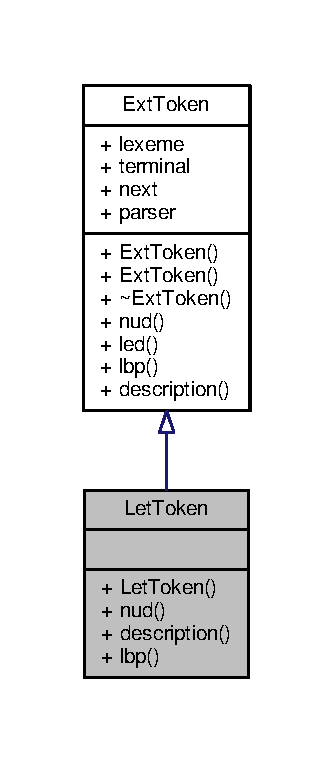
\includegraphics[width=160pt]{classLetToken__inherit__graph}
\end{center}
\end{figure}


Collaboration diagram for Let\-Token\-:\nopagebreak
\begin{figure}[H]
\begin{center}
\leavevmode
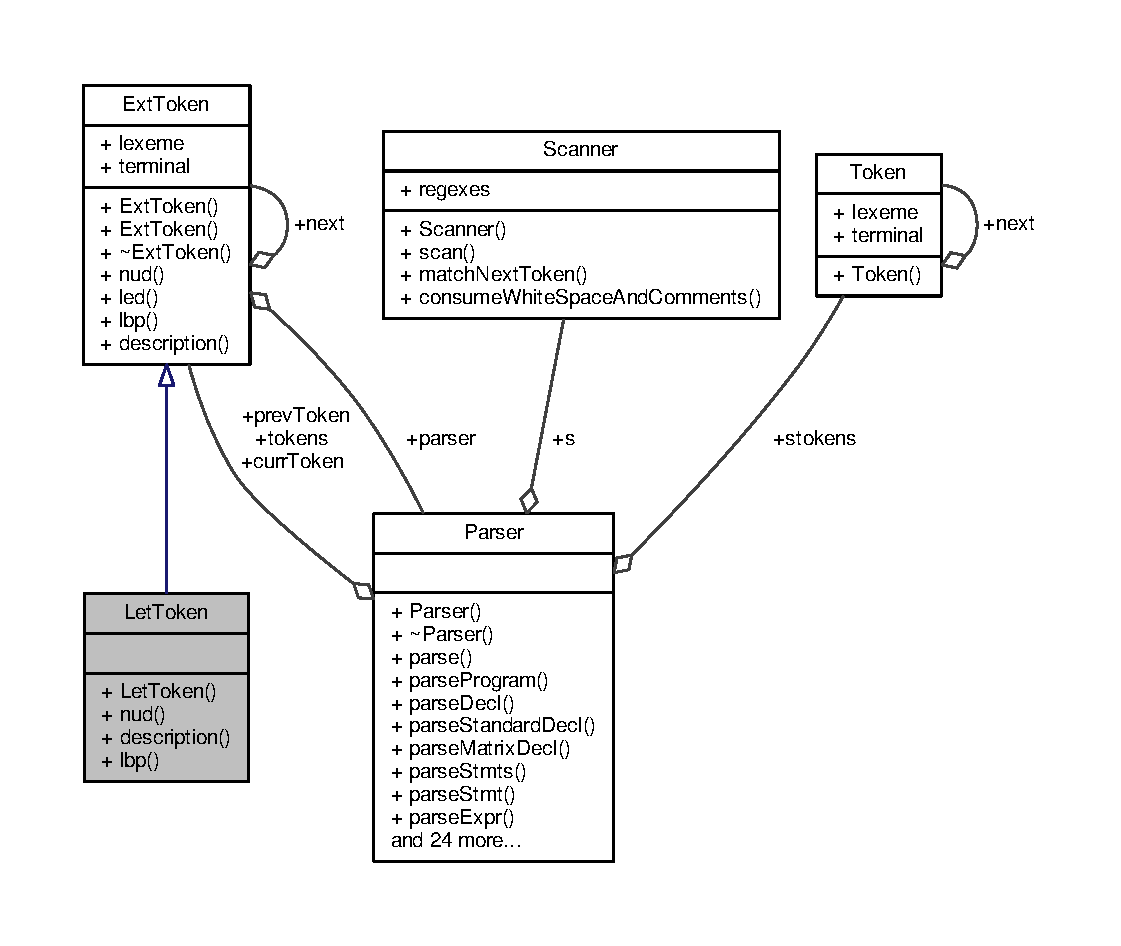
\includegraphics[width=350pt]{classLetToken__coll__graph}
\end{center}
\end{figure}
\subsection*{Public Member Functions}
\begin{DoxyCompactItemize}
\item 
\hyperlink{classLetToken_a94651a82207e47cd2c1066a58cb1fe08}{Let\-Token} (\hyperlink{classParser}{Parser} $\ast$p, \hyperlink{classToken}{Token} $\ast$t)
\item 
\hyperlink{classParseResult}{Parse\-Result} \hyperlink{classLetToken_a14df948cdf775bde8392bf58d53b91f3}{nud} ()
\item 
std\-::string \hyperlink{classLetToken_a2c5ba0489774bf6468a26f4e19d7fab4}{description} ()
\item 
int \hyperlink{classLetToken_a2a5ab5bc5897340513480c162bb2b065}{lbp} ()
\end{DoxyCompactItemize}
\subsection*{Additional Inherited Members}


\subsection{Constructor \& Destructor Documentation}
\hypertarget{classLetToken_a94651a82207e47cd2c1066a58cb1fe08}{\index{Let\-Token@{Let\-Token}!Let\-Token@{Let\-Token}}
\index{Let\-Token@{Let\-Token}!LetToken@{Let\-Token}}
\subsubsection[{Let\-Token}]{\setlength{\rightskip}{0pt plus 5cm}Let\-Token\-::\-Let\-Token (
\begin{DoxyParamCaption}
\item[{{\bf Parser} $\ast$}]{p, }
\item[{{\bf Token} $\ast$}]{t}
\end{DoxyParamCaption}
)\hspace{0.3cm}{\ttfamily [inline]}}}\label{classLetToken_a94651a82207e47cd2c1066a58cb1fe08}


\subsection{Member Function Documentation}
\hypertarget{classLetToken_a2c5ba0489774bf6468a26f4e19d7fab4}{\index{Let\-Token@{Let\-Token}!description@{description}}
\index{description@{description}!LetToken@{Let\-Token}}
\subsubsection[{description}]{\setlength{\rightskip}{0pt plus 5cm}std\-::string Let\-Token\-::description (
\begin{DoxyParamCaption}
{}
\end{DoxyParamCaption}
)\hspace{0.3cm}{\ttfamily [inline]}, {\ttfamily [virtual]}}}\label{classLetToken_a2c5ba0489774bf6468a26f4e19d7fab4}


Reimplemented from \hyperlink{classExtToken_a4ab6e72ac23235650b1756f794172ebb}{Ext\-Token}.

\hypertarget{classLetToken_a2a5ab5bc5897340513480c162bb2b065}{\index{Let\-Token@{Let\-Token}!lbp@{lbp}}
\index{lbp@{lbp}!LetToken@{Let\-Token}}
\subsubsection[{lbp}]{\setlength{\rightskip}{0pt plus 5cm}int Let\-Token\-::lbp (
\begin{DoxyParamCaption}
{}
\end{DoxyParamCaption}
)\hspace{0.3cm}{\ttfamily [inline]}, {\ttfamily [virtual]}}}\label{classLetToken_a2a5ab5bc5897340513480c162bb2b065}


Reimplemented from \hyperlink{classExtToken_a6c0d61faa058b71147dd54bacee1db94}{Ext\-Token}.

\hypertarget{classLetToken_a14df948cdf775bde8392bf58d53b91f3}{\index{Let\-Token@{Let\-Token}!nud@{nud}}
\index{nud@{nud}!LetToken@{Let\-Token}}
\subsubsection[{nud}]{\setlength{\rightskip}{0pt plus 5cm}{\bf Parse\-Result} Let\-Token\-::nud (
\begin{DoxyParamCaption}
{}
\end{DoxyParamCaption}
)\hspace{0.3cm}{\ttfamily [inline]}, {\ttfamily [virtual]}}}\label{classLetToken_a14df948cdf775bde8392bf58d53b91f3}


Reimplemented from \hyperlink{classExtToken_a5c21a5ffe91f212085259126652ab77c}{Ext\-Token}.



The documentation for this class was generated from the following file\-:\begin{DoxyCompactItemize}
\item 
\hyperlink{extToken_8h}{ext\-Token.\-h}\end{DoxyCompactItemize}

\hypertarget{classMatrixAdvDecl}{\section{Matrix\-Adv\-Decl Class Reference}
\label{classMatrixAdvDecl}\index{Matrix\-Adv\-Decl@{Matrix\-Adv\-Decl}}
}


Represents a declaration of a matrix with initial values. \par
  




{\ttfamily \#include $<$A\-S\-T.\-h$>$}



Inheritance diagram for Matrix\-Adv\-Decl\-:\nopagebreak
\begin{figure}[H]
\begin{center}
\leavevmode
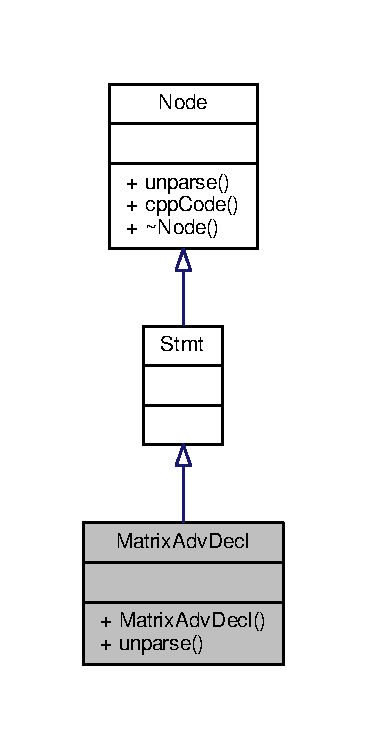
\includegraphics[width=176pt]{classMatrixAdvDecl__inherit__graph}
\end{center}
\end{figure}


Collaboration diagram for Matrix\-Adv\-Decl\-:\nopagebreak
\begin{figure}[H]
\begin{center}
\leavevmode
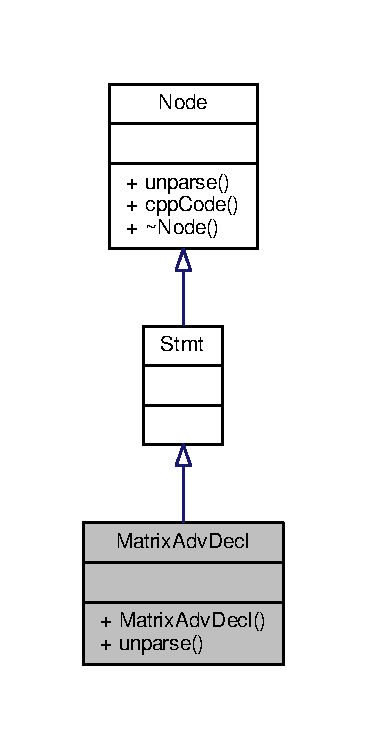
\includegraphics[width=176pt]{classMatrixAdvDecl__coll__graph}
\end{center}
\end{figure}
\subsection*{Public Member Functions}
\begin{DoxyCompactItemize}
\item 
\hyperlink{classMatrixAdvDecl_af91ad882300c22394ae4e203452985ce}{Matrix\-Adv\-Decl} (\hyperlink{classVarName}{Var\-Name} $\ast$v1, \hyperlink{classVarName}{Var\-Name} $\ast$v2, \hyperlink{classVarName}{Var\-Name} $\ast$v3, \hyperlink{classExpr}{Expr} $\ast$e1, \hyperlink{classExpr}{Expr} $\ast$e2, \hyperlink{classExpr}{Expr} $\ast$e3)
\item 
std\-::string \hyperlink{classMatrixAdvDecl_afa5f531b97e350e9a8c434bf5bdf1a0d}{unparse} ()
\begin{DoxyCompactList}\small\item\em Returns a string representation of the code modeled by this class and all its variables. \end{DoxyCompactList}\end{DoxyCompactItemize}


\subsection{Detailed Description}
Represents a declaration of a matrix with initial values. \par
 

Model\-: Decl \-:\-:= 'Matrix' var\-Name '\mbox{[}' \hyperlink{classExpr}{Expr} ',' \hyperlink{classExpr}{Expr} '\mbox{]}' var\-Name ',' var\-Name '=' \hyperlink{classExpr}{Expr} ';' \par
 Example\-: Matrix n\mbox{[}10,10\mbox{]} ni, ni = mi + mj; 

\subsection{Constructor \& Destructor Documentation}
\hypertarget{classMatrixAdvDecl_af91ad882300c22394ae4e203452985ce}{\index{Matrix\-Adv\-Decl@{Matrix\-Adv\-Decl}!Matrix\-Adv\-Decl@{Matrix\-Adv\-Decl}}
\index{Matrix\-Adv\-Decl@{Matrix\-Adv\-Decl}!MatrixAdvDecl@{Matrix\-Adv\-Decl}}
\subsubsection[{Matrix\-Adv\-Decl}]{\setlength{\rightskip}{0pt plus 5cm}Matrix\-Adv\-Decl\-::\-Matrix\-Adv\-Decl (
\begin{DoxyParamCaption}
\item[{{\bf Var\-Name} $\ast$}]{v1, }
\item[{{\bf Var\-Name} $\ast$}]{v2, }
\item[{{\bf Var\-Name} $\ast$}]{v3, }
\item[{{\bf Expr} $\ast$}]{e1, }
\item[{{\bf Expr} $\ast$}]{e2, }
\item[{{\bf Expr} $\ast$}]{e3}
\end{DoxyParamCaption}
)\hspace{0.3cm}{\ttfamily [inline]}}}\label{classMatrixAdvDecl_af91ad882300c22394ae4e203452985ce}
Public constructor. 
\begin{DoxyParams}{Parameters}
{\em v1} & -\/ Name of matrix being constructed \\
\hline
{\em v2} & -\/ First index variable name \\
\hline
{\em v3} & -\/ Second index variable name \\
\hline
{\em e1} & -\/ Row index expression \\
\hline
{\em e2} & -\/ Col index expression \\
\hline
{\em e3} & -\/ \hyperlink{classExpr}{Expr} for value to be assigned \\
\hline
\end{DoxyParams}


\subsection{Member Function Documentation}
\hypertarget{classMatrixAdvDecl_afa5f531b97e350e9a8c434bf5bdf1a0d}{\index{Matrix\-Adv\-Decl@{Matrix\-Adv\-Decl}!unparse@{unparse}}
\index{unparse@{unparse}!MatrixAdvDecl@{Matrix\-Adv\-Decl}}
\subsubsection[{unparse}]{\setlength{\rightskip}{0pt plus 5cm}string Matrix\-Adv\-Decl\-::unparse (
\begin{DoxyParamCaption}
{}
\end{DoxyParamCaption}
)\hspace{0.3cm}{\ttfamily [virtual]}}}\label{classMatrixAdvDecl_afa5f531b97e350e9a8c434bf5bdf1a0d}


Returns a string representation of the code modeled by this class and all its variables. 

\begin{DoxyReturn}{Returns}
std\-::string. 
\end{DoxyReturn}


Implements \hyperlink{classNode_a60ea533e0900961c05e701db70097136}{Node}.



The documentation for this class was generated from the following files\-:\begin{DoxyCompactItemize}
\item 
\hyperlink{AST_8h}{A\-S\-T.\-h}\item 
\hyperlink{AST_8cpp}{A\-S\-T.\-cpp}\end{DoxyCompactItemize}

\hypertarget{classMatrixAssignStmt}{\section{Matrix\-Assign\-Stmt Class Reference}
\label{classMatrixAssignStmt}\index{Matrix\-Assign\-Stmt@{Matrix\-Assign\-Stmt}}
}


Represents a matrix assignment. \par
  




{\ttfamily \#include $<$A\-S\-T.\-h$>$}



Inheritance diagram for Matrix\-Assign\-Stmt\-:\nopagebreak
\begin{figure}[H]
\begin{center}
\leavevmode
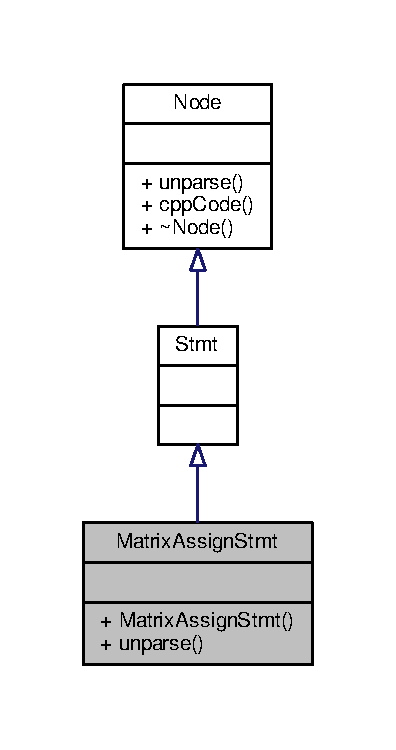
\includegraphics[width=190pt]{classMatrixAssignStmt__inherit__graph}
\end{center}
\end{figure}


Collaboration diagram for Matrix\-Assign\-Stmt\-:\nopagebreak
\begin{figure}[H]
\begin{center}
\leavevmode
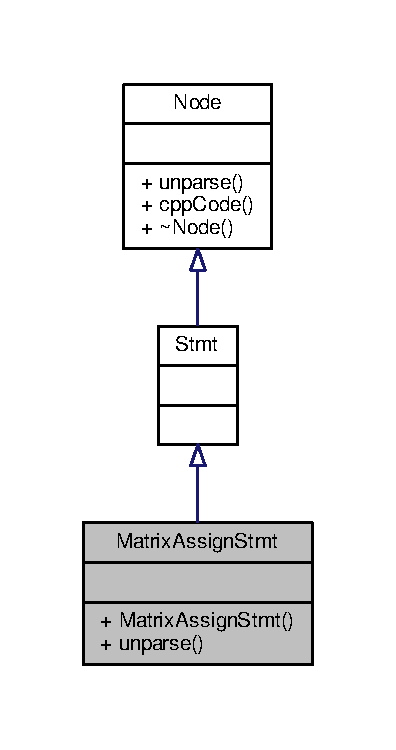
\includegraphics[width=190pt]{classMatrixAssignStmt__coll__graph}
\end{center}
\end{figure}
\subsection*{Public Member Functions}
\begin{DoxyCompactItemize}
\item 
\hyperlink{classMatrixAssignStmt_aa68d9d5e2febd0e7378fa8ce9433276e}{Matrix\-Assign\-Stmt} (\hyperlink{classVarName}{Var\-Name} $\ast$v, \hyperlink{classExpr}{Expr} $\ast$e1, \hyperlink{classExpr}{Expr} $\ast$e2, \hyperlink{classExpr}{Expr} $\ast$e3)
\item 
std\-::string \hyperlink{classMatrixAssignStmt_a7eb7f14cd0efb9a8fbe6a463a5f5a7cf}{unparse} ()
\begin{DoxyCompactList}\small\item\em Returns a string representation of the code modeled by this class and all its variables. \end{DoxyCompactList}\end{DoxyCompactItemize}


\subsection{Detailed Description}
Represents a matrix assignment. \par
 

Model\-: var\-Name '\mbox{[}' \hyperlink{classExpr}{Expr} ',' \hyperlink{classExpr}{Expr} '\mbox{]}' '=' \hyperlink{classExpr}{Expr} ';' \par
 Example\-: matrix\mbox{[}0,0\mbox{]} = 8; 

\subsection{Constructor \& Destructor Documentation}
\hypertarget{classMatrixAssignStmt_aa68d9d5e2febd0e7378fa8ce9433276e}{\index{Matrix\-Assign\-Stmt@{Matrix\-Assign\-Stmt}!Matrix\-Assign\-Stmt@{Matrix\-Assign\-Stmt}}
\index{Matrix\-Assign\-Stmt@{Matrix\-Assign\-Stmt}!MatrixAssignStmt@{Matrix\-Assign\-Stmt}}
\subsubsection[{Matrix\-Assign\-Stmt}]{\setlength{\rightskip}{0pt plus 5cm}Matrix\-Assign\-Stmt\-::\-Matrix\-Assign\-Stmt (
\begin{DoxyParamCaption}
\item[{{\bf Var\-Name} $\ast$}]{v, }
\item[{{\bf Expr} $\ast$}]{e1, }
\item[{{\bf Expr} $\ast$}]{e2, }
\item[{{\bf Expr} $\ast$}]{e3}
\end{DoxyParamCaption}
)\hspace{0.3cm}{\ttfamily [inline]}}}\label{classMatrixAssignStmt_aa68d9d5e2febd0e7378fa8ce9433276e}
Public constructor. 
\begin{DoxyParams}{Parameters}
{\em v} & -\/ Name of matrix being assigned \\
\hline
{\em e1} & -\/ Expression of the value of the row to be assigned \\
\hline
{\em e2} & -\/ Expression of the value to the col to be assigned \\
\hline
{\em e3} & -\/ Expression of the value to be assigned \\
\hline
\end{DoxyParams}


\subsection{Member Function Documentation}
\hypertarget{classMatrixAssignStmt_a7eb7f14cd0efb9a8fbe6a463a5f5a7cf}{\index{Matrix\-Assign\-Stmt@{Matrix\-Assign\-Stmt}!unparse@{unparse}}
\index{unparse@{unparse}!MatrixAssignStmt@{Matrix\-Assign\-Stmt}}
\subsubsection[{unparse}]{\setlength{\rightskip}{0pt plus 5cm}string Matrix\-Assign\-Stmt\-::unparse (
\begin{DoxyParamCaption}
{}
\end{DoxyParamCaption}
)\hspace{0.3cm}{\ttfamily [virtual]}}}\label{classMatrixAssignStmt_a7eb7f14cd0efb9a8fbe6a463a5f5a7cf}


Returns a string representation of the code modeled by this class and all its variables. 

\begin{DoxyReturn}{Returns}
std\-::string. 
\end{DoxyReturn}


Implements \hyperlink{classNode_a60ea533e0900961c05e701db70097136}{Node}.



The documentation for this class was generated from the following files\-:\begin{DoxyCompactItemize}
\item 
\hyperlink{AST_8h}{A\-S\-T.\-h}\item 
\hyperlink{AST_8cpp}{A\-S\-T.\-cpp}\end{DoxyCompactItemize}

\hypertarget{classMatrixDecl}{\section{Matrix\-Decl Class Reference}
\label{classMatrixDecl}\index{Matrix\-Decl@{Matrix\-Decl}}
}


Represents a standard declaration of a matrix. \par
  




{\ttfamily \#include $<$A\-S\-T.\-h$>$}



Inheritance diagram for Matrix\-Decl\-:\nopagebreak
\begin{figure}[H]
\begin{center}
\leavevmode
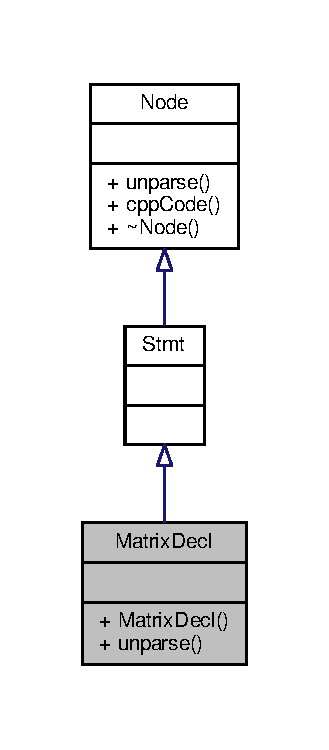
\includegraphics[width=158pt]{classMatrixDecl__inherit__graph}
\end{center}
\end{figure}


Collaboration diagram for Matrix\-Decl\-:\nopagebreak
\begin{figure}[H]
\begin{center}
\leavevmode
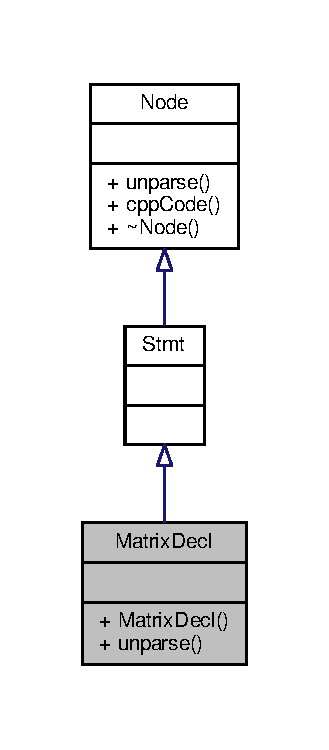
\includegraphics[width=158pt]{classMatrixDecl__coll__graph}
\end{center}
\end{figure}
\subsection*{Public Member Functions}
\begin{DoxyCompactItemize}
\item 
\hyperlink{classMatrixDecl_a8547ecfc238547a828bc43374fe42833}{Matrix\-Decl} (\hyperlink{classVarName}{Var\-Name} $\ast$v, \hyperlink{classExpr}{Expr} $\ast$e)
\item 
std\-::string \hyperlink{classMatrixDecl_a060b7cc8af5fd4cb10e045321b39d397}{unparse} ()
\begin{DoxyCompactList}\small\item\em Returns a string representation of the code modeled by this class and all its variables. \end{DoxyCompactList}\end{DoxyCompactItemize}


\subsection{Detailed Description}
Represents a standard declaration of a matrix. \par
 

Model\-: Decl \-:\-:= 'Matrix' var\-Name '=' \hyperlink{classExpr}{Expr} ';' \par
 Example\-: Matrix new\-\_\-matrix = 10; 

\subsection{Constructor \& Destructor Documentation}
\hypertarget{classMatrixDecl_a8547ecfc238547a828bc43374fe42833}{\index{Matrix\-Decl@{Matrix\-Decl}!Matrix\-Decl@{Matrix\-Decl}}
\index{Matrix\-Decl@{Matrix\-Decl}!MatrixDecl@{Matrix\-Decl}}
\subsubsection[{Matrix\-Decl}]{\setlength{\rightskip}{0pt plus 5cm}Matrix\-Decl\-::\-Matrix\-Decl (
\begin{DoxyParamCaption}
\item[{{\bf Var\-Name} $\ast$}]{v, }
\item[{{\bf Expr} $\ast$}]{e}
\end{DoxyParamCaption}
)\hspace{0.3cm}{\ttfamily [inline]}}}\label{classMatrixDecl_a8547ecfc238547a828bc43374fe42833}
Public constructor. 
\begin{DoxyParams}{Parameters}
{\em v} & -\/ Name of matrix being constructed \\
\hline
{\em e} & -\/ \hyperlink{classExpr}{Expr} of value being assigned \\
\hline
\end{DoxyParams}


\subsection{Member Function Documentation}
\hypertarget{classMatrixDecl_a060b7cc8af5fd4cb10e045321b39d397}{\index{Matrix\-Decl@{Matrix\-Decl}!unparse@{unparse}}
\index{unparse@{unparse}!MatrixDecl@{Matrix\-Decl}}
\subsubsection[{unparse}]{\setlength{\rightskip}{0pt plus 5cm}string Matrix\-Decl\-::unparse (
\begin{DoxyParamCaption}
{}
\end{DoxyParamCaption}
)\hspace{0.3cm}{\ttfamily [virtual]}}}\label{classMatrixDecl_a060b7cc8af5fd4cb10e045321b39d397}


Returns a string representation of the code modeled by this class and all its variables. 

\begin{DoxyReturn}{Returns}
std\-::string. 
\end{DoxyReturn}


Implements \hyperlink{classNode_a60ea533e0900961c05e701db70097136}{Node}.



The documentation for this class was generated from the following files\-:\begin{DoxyCompactItemize}
\item 
\hyperlink{AST_8h}{A\-S\-T.\-h}\item 
\hyperlink{AST_8cpp}{A\-S\-T.\-cpp}\end{DoxyCompactItemize}

\hypertarget{classMatrixRefExpr}{\section{Matrix\-Ref\-Expr Class Reference}
\label{classMatrixRefExpr}\index{Matrix\-Ref\-Expr@{Matrix\-Ref\-Expr}}
}


Represents accessing a matrix. \par
  




{\ttfamily \#include $<$A\-S\-T.\-h$>$}



Inheritance diagram for Matrix\-Ref\-Expr\-:\nopagebreak
\begin{figure}[H]
\begin{center}
\leavevmode
\includegraphics[width=174pt]{classMatrixRefExpr__inherit__graph}
\end{center}
\end{figure}


Collaboration diagram for Matrix\-Ref\-Expr\-:\nopagebreak
\begin{figure}[H]
\begin{center}
\leavevmode
\includegraphics[width=174pt]{classMatrixRefExpr__coll__graph}
\end{center}
\end{figure}
\subsection*{Public Member Functions}
\begin{DoxyCompactItemize}
\item 
\hyperlink{classMatrixRefExpr_a70075a049a62f4115f9964206ca3da1e}{Matrix\-Ref\-Expr} (\hyperlink{classVarName}{Var\-Name} $\ast$v, \hyperlink{classExpr}{Expr} $\ast$e1, \hyperlink{classExpr}{Expr} $\ast$e2)
\item 
std\-::string \hyperlink{classMatrixRefExpr_ae1026da77ca12726f14e2f61656a22d8}{unparse} ()
\begin{DoxyCompactList}\small\item\em Returns a string representation of the code modeled by this class and all its variables. \end{DoxyCompactList}\end{DoxyCompactItemize}


\subsection{Detailed Description}
Represents accessing a matrix. \par
 

Model\-: \hyperlink{classExpr}{Expr} \-:\-:= var\-Name '\mbox{[}' \hyperlink{classExpr}{Expr} ',' \hyperlink{classExpr}{Expr} '\mbox{]}' \par
 Example\-: matrix\mbox{[}0.\-0\mbox{]} 

\subsection{Constructor \& Destructor Documentation}
\hypertarget{classMatrixRefExpr_a70075a049a62f4115f9964206ca3da1e}{\index{Matrix\-Ref\-Expr@{Matrix\-Ref\-Expr}!Matrix\-Ref\-Expr@{Matrix\-Ref\-Expr}}
\index{Matrix\-Ref\-Expr@{Matrix\-Ref\-Expr}!MatrixRefExpr@{Matrix\-Ref\-Expr}}
\subsubsection[{Matrix\-Ref\-Expr}]{\setlength{\rightskip}{0pt plus 5cm}Matrix\-Ref\-Expr\-::\-Matrix\-Ref\-Expr (
\begin{DoxyParamCaption}
\item[{{\bf Var\-Name} $\ast$}]{v, }
\item[{{\bf Expr} $\ast$}]{e1, }
\item[{{\bf Expr} $\ast$}]{e2}
\end{DoxyParamCaption}
)\hspace{0.3cm}{\ttfamily [inline]}}}\label{classMatrixRefExpr_a70075a049a62f4115f9964206ca3da1e}
Public constructor. 
\begin{DoxyParams}{Parameters}
{\em v} & -\/ Name of matrix being accessed \\
\hline
{\em e1} & -\/ Expression of row being accessed \\
\hline
{\em e2} & -\/ Expression of col being accessed \\
\hline
\end{DoxyParams}


\subsection{Member Function Documentation}
\hypertarget{classMatrixRefExpr_ae1026da77ca12726f14e2f61656a22d8}{\index{Matrix\-Ref\-Expr@{Matrix\-Ref\-Expr}!unparse@{unparse}}
\index{unparse@{unparse}!MatrixRefExpr@{Matrix\-Ref\-Expr}}
\subsubsection[{unparse}]{\setlength{\rightskip}{0pt plus 5cm}string Matrix\-Ref\-Expr\-::unparse (
\begin{DoxyParamCaption}
{}
\end{DoxyParamCaption}
)\hspace{0.3cm}{\ttfamily [virtual]}}}\label{classMatrixRefExpr_ae1026da77ca12726f14e2f61656a22d8}


Returns a string representation of the code modeled by this class and all its variables. 

\begin{DoxyReturn}{Returns}
std\-::string. 
\end{DoxyReturn}


Implements \hyperlink{classNode_a60ea533e0900961c05e701db70097136}{Node}.



The documentation for this class was generated from the following files\-:\begin{DoxyCompactItemize}
\item 
\hyperlink{AST_8h}{A\-S\-T.\-h}\item 
\hyperlink{AST_8cpp}{A\-S\-T.\-cpp}\end{DoxyCompactItemize}

\hypertarget{classNode}{\section{Node Class Reference}
\label{classNode}\index{Node@{Node}}
}


Abstract parent or grandparent for all classes in the Abstract Syntax Tree (A\-S\-T)  




{\ttfamily \#include $<$A\-S\-T.\-h$>$}



Inheritance diagram for Node\-:
\nopagebreak
\begin{figure}[H]
\begin{center}
\leavevmode
\includegraphics[width=350pt]{classNode__inherit__graph}
\end{center}
\end{figure}


Collaboration diagram for Node\-:\nopagebreak
\begin{figure}[H]
\begin{center}
\leavevmode
\includegraphics[width=150pt]{classNode__coll__graph}
\end{center}
\end{figure}
\subsection*{Public Member Functions}
\begin{DoxyCompactItemize}
\item 
virtual std\-::string \hyperlink{classNode_a60ea533e0900961c05e701db70097136}{unparse} ()=0
\item 
virtual std\-::string \hyperlink{classNode_ab9dc8a0791d329231bc8427a7d7e9c2f}{cpp\-Code} ()
\item 
virtual \hyperlink{classNode_af5e3fa79300bf5f3f2f3ecae6e795a94}{$\sim$\-Node} ()
\end{DoxyCompactItemize}


\subsection{Detailed Description}
Abstract parent or grandparent for all classes in the Abstract Syntax Tree (A\-S\-T) 

\subsection{Constructor \& Destructor Documentation}
\hypertarget{classNode_af5e3fa79300bf5f3f2f3ecae6e795a94}{\index{Node@{Node}!$\sim$\-Node@{$\sim$\-Node}}
\index{$\sim$\-Node@{$\sim$\-Node}!Node@{Node}}
\subsubsection[{$\sim$\-Node}]{\setlength{\rightskip}{0pt plus 5cm}virtual Node\-::$\sim$\-Node (
\begin{DoxyParamCaption}
{}
\end{DoxyParamCaption}
)\hspace{0.3cm}{\ttfamily [inline]}, {\ttfamily [virtual]}}}\label{classNode_af5e3fa79300bf5f3f2f3ecae6e795a94}


\subsection{Member Function Documentation}
\hypertarget{classNode_ab9dc8a0791d329231bc8427a7d7e9c2f}{\index{Node@{Node}!cpp\-Code@{cpp\-Code}}
\index{cpp\-Code@{cpp\-Code}!Node@{Node}}
\subsubsection[{cpp\-Code}]{\setlength{\rightskip}{0pt plus 5cm}virtual std\-::string Node\-::cpp\-Code (
\begin{DoxyParamCaption}
{}
\end{DoxyParamCaption}
)\hspace{0.3cm}{\ttfamily [inline]}, {\ttfamily [virtual]}}}\label{classNode_ab9dc8a0791d329231bc8427a7d7e9c2f}
\hypertarget{classNode_a60ea533e0900961c05e701db70097136}{\index{Node@{Node}!unparse@{unparse}}
\index{unparse@{unparse}!Node@{Node}}
\subsubsection[{unparse}]{\setlength{\rightskip}{0pt plus 5cm}virtual std\-::string Node\-::unparse (
\begin{DoxyParamCaption}
{}
\end{DoxyParamCaption}
)\hspace{0.3cm}{\ttfamily [pure virtual]}}}\label{classNode_a60ea533e0900961c05e701db70097136}


Implemented in \hyperlink{classNotExpr_aa1632e9a8abf6aa1bf110afed379066b}{Not\-Expr}, \hyperlink{classIfExpr_a4b4c34fffb9539bac51cf5eb35e30081}{If\-Expr}, \hyperlink{classLetExpr_a518a538c87aeec36204d8a465be32913}{Let\-Expr}, \hyperlink{classParensExpr_ad8eabc69cf42ce3ee92d88caeb40134a}{Parens\-Expr}, \hyperlink{classFunctionCall_aa80e938636e993ed9956e11a51858b95}{Function\-Call}, \hyperlink{classMatrixRefExpr_ae1026da77ca12726f14e2f61656a22d8}{Matrix\-Ref\-Expr}, \hyperlink{classBinOpExpr_a1ec35159c20a6b8481ee89ae5829c14d}{Bin\-Op\-Expr}, \hyperlink{classAnyConst_a2c4a9d1499b29bde8e72650cae459716}{Any\-Const}, \hyperlink{classVarName_aabc6d52ebde3abe413bd9a2d75a50f3c}{Var\-Name}, \hyperlink{classWhileStmt_a1fd1b12f4d16d898b9dcc647417057fa}{While\-Stmt}, \hyperlink{classForStmt_a9cf08250042ae5a0a54d2196b584e28e}{For\-Stmt}, \hyperlink{classPrintStmt_a7f80dc4ce628e16d32cb6f06a417a748}{Print\-Stmt}, \hyperlink{classMatrixAssignStmt_a7eb7f14cd0efb9a8fbe6a463a5f5a7cf}{Matrix\-Assign\-Stmt}, \hyperlink{classStandardAssignStmt_aa4bef62d90b49a7ed4c5120cb656ba0e}{Standard\-Assign\-Stmt}, \hyperlink{classIfElseStmt_a2e8c850644f33e4ba918c53d0212e59f}{If\-Else\-Stmt}, \hyperlink{classIfStmt_abc1ada72841299826de65fbdf5dc36a0}{If\-Stmt}, \hyperlink{classStmtBlock_add948dedcbf091739307aa977f0a027e}{Stmt\-Block}, \hyperlink{classMatrixDecl_a060b7cc8af5fd4cb10e045321b39d397}{Matrix\-Decl}, \hyperlink{classMatrixAdvDecl_afa5f531b97e350e9a8c434bf5bdf1a0d}{Matrix\-Adv\-Decl}, \hyperlink{classStandardDecl_a3ee30dee2f990e66c795a1fb77fe0117}{Standard\-Decl}, \hyperlink{classStmtStmts_ae1cfeb7d7f0c155c6be7b42614954a23}{Stmt\-Stmts}, \hyperlink{classEmptyStmts_a0f5a1640891e7c70f8ac38d6df031f0e}{Empty\-Stmts}, and \hyperlink{classRoot_a887fe7392c99899892838a032925525c}{Root}.



The documentation for this class was generated from the following file\-:\begin{DoxyCompactItemize}
\item 
\hyperlink{AST_8h}{A\-S\-T.\-h}\end{DoxyCompactItemize}

\hypertarget{classNotExpr}{\section{Not\-Expr Class Reference}
\label{classNotExpr}\index{Not\-Expr@{Not\-Expr}}
}


Represents negation of a boolean \par
  




{\ttfamily \#include $<$A\-S\-T.\-h$>$}



Inheritance diagram for Not\-Expr\-:\nopagebreak
\begin{figure}[H]
\begin{center}
\leavevmode
\includegraphics[width=150pt]{classNotExpr__inherit__graph}
\end{center}
\end{figure}


Collaboration diagram for Not\-Expr\-:\nopagebreak
\begin{figure}[H]
\begin{center}
\leavevmode
\includegraphics[width=150pt]{classNotExpr__coll__graph}
\end{center}
\end{figure}
\subsection*{Public Member Functions}
\begin{DoxyCompactItemize}
\item 
\hyperlink{classNotExpr_a7939cb5c7141f8ede498cef1e8f9694c}{Not\-Expr} (\hyperlink{classExpr}{Expr} $\ast$e)
\item 
std\-::string \hyperlink{classNotExpr_aa1632e9a8abf6aa1bf110afed379066b}{unparse} ()
\begin{DoxyCompactList}\small\item\em Returns a string representation of the code modeled by this class and all its variables. \end{DoxyCompactList}\end{DoxyCompactItemize}


\subsection{Detailed Description}
Represents negation of a boolean \par
 

Model\-: \hyperlink{classExpr}{Expr} \-:\-:= '!' \hyperlink{classExpr}{Expr} \par
 Example\-: !true 

\subsection{Constructor \& Destructor Documentation}
\hypertarget{classNotExpr_a7939cb5c7141f8ede498cef1e8f9694c}{\index{Not\-Expr@{Not\-Expr}!Not\-Expr@{Not\-Expr}}
\index{Not\-Expr@{Not\-Expr}!NotExpr@{Not\-Expr}}
\subsubsection[{Not\-Expr}]{\setlength{\rightskip}{0pt plus 5cm}Not\-Expr\-::\-Not\-Expr (
\begin{DoxyParamCaption}
\item[{{\bf Expr} $\ast$}]{e}
\end{DoxyParamCaption}
)\hspace{0.3cm}{\ttfamily [inline]}}}\label{classNotExpr_a7939cb5c7141f8ede498cef1e8f9694c}
Public constructor. 
\begin{DoxyParams}{Parameters}
{\em e} & -\/ Boolean expression being negated \\
\hline
\end{DoxyParams}


\subsection{Member Function Documentation}
\hypertarget{classNotExpr_aa1632e9a8abf6aa1bf110afed379066b}{\index{Not\-Expr@{Not\-Expr}!unparse@{unparse}}
\index{unparse@{unparse}!NotExpr@{Not\-Expr}}
\subsubsection[{unparse}]{\setlength{\rightskip}{0pt plus 5cm}string Not\-Expr\-::unparse (
\begin{DoxyParamCaption}
{}
\end{DoxyParamCaption}
)\hspace{0.3cm}{\ttfamily [virtual]}}}\label{classNotExpr_aa1632e9a8abf6aa1bf110afed379066b}


Returns a string representation of the code modeled by this class and all its variables. 

\begin{DoxyReturn}{Returns}
std\-::string. 
\end{DoxyReturn}


Implements \hyperlink{classNode_a60ea533e0900961c05e701db70097136}{Node}.



The documentation for this class was generated from the following files\-:\begin{DoxyCompactItemize}
\item 
\hyperlink{AST_8h}{A\-S\-T.\-h}\item 
\hyperlink{AST_8cpp}{A\-S\-T.\-cpp}\end{DoxyCompactItemize}

\hypertarget{classNotOpToken}{\section{Not\-Op\-Token Class Reference}
\label{classNotOpToken}\index{Not\-Op\-Token@{Not\-Op\-Token}}
}


{\ttfamily \#include $<$ext\-Token.\-h$>$}



Inheritance diagram for Not\-Op\-Token\-:\nopagebreak
\begin{figure}[H]
\begin{center}
\leavevmode
\includegraphics[width=166pt]{classNotOpToken__inherit__graph}
\end{center}
\end{figure}


Collaboration diagram for Not\-Op\-Token\-:\nopagebreak
\begin{figure}[H]
\begin{center}
\leavevmode
\includegraphics[width=350pt]{classNotOpToken__coll__graph}
\end{center}
\end{figure}
\subsection*{Public Member Functions}
\begin{DoxyCompactItemize}
\item 
\hyperlink{classNotOpToken_afb8b9e96a178b1dfd69abf0a901dfddf}{Not\-Op\-Token} (\hyperlink{classParser}{Parser} $\ast$p, \hyperlink{classToken}{Token} $\ast$t)
\item 
\hyperlink{classParseResult}{Parse\-Result} \hyperlink{classNotOpToken_a55a0dd53742aaca04338c16be079b031}{nud} ()
\item 
std\-::string \hyperlink{classNotOpToken_a136a11f1e42542a9a58b7c14249c9d23}{description} ()
\end{DoxyCompactItemize}
\subsection*{Additional Inherited Members}


\subsection{Constructor \& Destructor Documentation}
\hypertarget{classNotOpToken_afb8b9e96a178b1dfd69abf0a901dfddf}{\index{Not\-Op\-Token@{Not\-Op\-Token}!Not\-Op\-Token@{Not\-Op\-Token}}
\index{Not\-Op\-Token@{Not\-Op\-Token}!NotOpToken@{Not\-Op\-Token}}
\subsubsection[{Not\-Op\-Token}]{\setlength{\rightskip}{0pt plus 5cm}Not\-Op\-Token\-::\-Not\-Op\-Token (
\begin{DoxyParamCaption}
\item[{{\bf Parser} $\ast$}]{p, }
\item[{{\bf Token} $\ast$}]{t}
\end{DoxyParamCaption}
)\hspace{0.3cm}{\ttfamily [inline]}}}\label{classNotOpToken_afb8b9e96a178b1dfd69abf0a901dfddf}


\subsection{Member Function Documentation}
\hypertarget{classNotOpToken_a136a11f1e42542a9a58b7c14249c9d23}{\index{Not\-Op\-Token@{Not\-Op\-Token}!description@{description}}
\index{description@{description}!NotOpToken@{Not\-Op\-Token}}
\subsubsection[{description}]{\setlength{\rightskip}{0pt plus 5cm}std\-::string Not\-Op\-Token\-::description (
\begin{DoxyParamCaption}
{}
\end{DoxyParamCaption}
)\hspace{0.3cm}{\ttfamily [inline]}, {\ttfamily [virtual]}}}\label{classNotOpToken_a136a11f1e42542a9a58b7c14249c9d23}


Reimplemented from \hyperlink{classExtToken_a4ab6e72ac23235650b1756f794172ebb}{Ext\-Token}.

\hypertarget{classNotOpToken_a55a0dd53742aaca04338c16be079b031}{\index{Not\-Op\-Token@{Not\-Op\-Token}!nud@{nud}}
\index{nud@{nud}!NotOpToken@{Not\-Op\-Token}}
\subsubsection[{nud}]{\setlength{\rightskip}{0pt plus 5cm}{\bf Parse\-Result} Not\-Op\-Token\-::nud (
\begin{DoxyParamCaption}
{}
\end{DoxyParamCaption}
)\hspace{0.3cm}{\ttfamily [inline]}, {\ttfamily [virtual]}}}\label{classNotOpToken_a55a0dd53742aaca04338c16be079b031}


Reimplemented from \hyperlink{classExtToken_a5c21a5ffe91f212085259126652ab77c}{Ext\-Token}.



The documentation for this class was generated from the following file\-:\begin{DoxyCompactItemize}
\item 
\hyperlink{extToken_8h}{ext\-Token.\-h}\end{DoxyCompactItemize}

\hypertarget{classParensExpr}{\section{Parens\-Expr Class Reference}
\label{classParensExpr}\index{Parens\-Expr@{Parens\-Expr}}
}


Represents an expression surrounded by parenthesis. \par
  




{\ttfamily \#include $<$A\-S\-T.\-h$>$}



Inheritance diagram for Parens\-Expr\-:\nopagebreak
\begin{figure}[H]
\begin{center}
\leavevmode
\includegraphics[width=162pt]{classParensExpr__inherit__graph}
\end{center}
\end{figure}


Collaboration diagram for Parens\-Expr\-:\nopagebreak
\begin{figure}[H]
\begin{center}
\leavevmode
\includegraphics[width=162pt]{classParensExpr__coll__graph}
\end{center}
\end{figure}
\subsection*{Public Member Functions}
\begin{DoxyCompactItemize}
\item 
\hyperlink{classParensExpr_a1f690170bb62040a48c38df1aef7a453}{Parens\-Expr} (\hyperlink{classExpr}{Expr} $\ast$e)
\item 
std\-::string \hyperlink{classParensExpr_ad8eabc69cf42ce3ee92d88caeb40134a}{unparse} ()
\begin{DoxyCompactList}\small\item\em Returns a string representation of the code modeled by this class and all its variables. \end{DoxyCompactList}\end{DoxyCompactItemize}


\subsection{Detailed Description}
Represents an expression surrounded by parenthesis. \par
 

Model\-: \hyperlink{classExpr}{Expr} \-:\-:= '(' \hyperlink{classExpr}{Expr} ')' \par
 Example\-: (1 + 1) 

\subsection{Constructor \& Destructor Documentation}
\hypertarget{classParensExpr_a1f690170bb62040a48c38df1aef7a453}{\index{Parens\-Expr@{Parens\-Expr}!Parens\-Expr@{Parens\-Expr}}
\index{Parens\-Expr@{Parens\-Expr}!ParensExpr@{Parens\-Expr}}
\subsubsection[{Parens\-Expr}]{\setlength{\rightskip}{0pt plus 5cm}Parens\-Expr\-::\-Parens\-Expr (
\begin{DoxyParamCaption}
\item[{{\bf Expr} $\ast$}]{e}
\end{DoxyParamCaption}
)\hspace{0.3cm}{\ttfamily [inline]}}}\label{classParensExpr_a1f690170bb62040a48c38df1aef7a453}
Public constructor. 
\begin{DoxyParams}{Parameters}
{\em e} & -\/ Expression evaluated inside the parenthesis \\
\hline
\end{DoxyParams}


\subsection{Member Function Documentation}
\hypertarget{classParensExpr_ad8eabc69cf42ce3ee92d88caeb40134a}{\index{Parens\-Expr@{Parens\-Expr}!unparse@{unparse}}
\index{unparse@{unparse}!ParensExpr@{Parens\-Expr}}
\subsubsection[{unparse}]{\setlength{\rightskip}{0pt plus 5cm}string Parens\-Expr\-::unparse (
\begin{DoxyParamCaption}
{}
\end{DoxyParamCaption}
)\hspace{0.3cm}{\ttfamily [virtual]}}}\label{classParensExpr_ad8eabc69cf42ce3ee92d88caeb40134a}


Returns a string representation of the code modeled by this class and all its variables. 

\begin{DoxyReturn}{Returns}
std\-::string. 
\end{DoxyReturn}


Implements \hyperlink{classNode_a60ea533e0900961c05e701db70097136}{Node}.



The documentation for this class was generated from the following files\-:\begin{DoxyCompactItemize}
\item 
\hyperlink{AST_8h}{A\-S\-T.\-h}\item 
\hyperlink{AST_8cpp}{A\-S\-T.\-cpp}\end{DoxyCompactItemize}

\hypertarget{classParser}{\section{Parser Class Reference}
\label{classParser}\index{Parser@{Parser}}
}


Organizes F\-C\-A\-L text into an tree.  




{\ttfamily \#include $<$parser.\-h$>$}



Collaboration diagram for Parser\-:\nopagebreak
\begin{figure}[H]
\begin{center}
\leavevmode
\includegraphics[width=350pt]{classParser__coll__graph}
\end{center}
\end{figure}
\subsection*{Public Member Functions}
\begin{DoxyCompactItemize}
\item 
\hyperlink{classParser_a12234f6cd36b61af4b50c94a179422c1}{Parser} ()
\begin{DoxyCompactList}\small\item\em Default constructor. Sets everything to N\-U\-L\-L. \end{DoxyCompactList}\item 
\hyperlink{classParser_a3e658b5917a93a3ef648050d060e3a93}{$\sim$\-Parser} ()
\begin{DoxyCompactList}\small\item\em Default destructor. \end{DoxyCompactList}\item 
\hyperlink{classParseResult}{Parse\-Result} \hyperlink{classParser_a2c1a7aa0b09a43bc1eef460817efb1d6}{parse} (const char $\ast$text)
\begin{DoxyCompactList}\small\item\em Parses the program. \end{DoxyCompactList}\item 
\hyperlink{classParseResult}{Parse\-Result} \hyperlink{classParser_a14e25c84322809e2f060dc530362ea71}{parse\-Program} ()
\begin{DoxyCompactList}\small\item\em Parses the program. \end{DoxyCompactList}\item 
\hyperlink{classParseResult}{Parse\-Result} \hyperlink{classParser_ac646227983887c1cd13dae67fa1bc142}{parse\-Decl} ()
\begin{DoxyCompactList}\small\item\em Parses declarations of variables. \end{DoxyCompactList}\item 
\hyperlink{classParseResult}{Parse\-Result} \hyperlink{classParser_a1e1f83c0f4b11148a356d951f191425e}{parse\-Standard\-Decl} ()
\begin{DoxyCompactList}\small\item\em Parses a standard declaration of a variable. \end{DoxyCompactList}\item 
\hyperlink{classParseResult}{Parse\-Result} \hyperlink{classParser_a3a00df25fda2af308b69f05eed14ac69}{parse\-Matrix\-Decl} ()
\begin{DoxyCompactList}\small\item\em Parses a Matrix Declaration. \end{DoxyCompactList}\item 
\hyperlink{classParseResult}{Parse\-Result} \hyperlink{classParser_a452db3def31683cb0305e57a01489bd4}{parse\-Stmts} ()
\begin{DoxyCompactList}\small\item\em Starting place to parse any type of \hyperlink{classStmts}{Stmts}. \end{DoxyCompactList}\item 
\hyperlink{classParseResult}{Parse\-Result} \hyperlink{classParser_a9709c4793d0cce012d595f3ee416cd25}{parse\-Stmt} ()
\begin{DoxyCompactList}\small\item\em Starting place to parse any type of \hyperlink{classStmt}{Stmt}. \end{DoxyCompactList}\item 
\hyperlink{classParseResult}{Parse\-Result} \hyperlink{classParser_a50227dc24dc7a175ac0533d9957dfcf8}{parse\-Expr} (int rbp)
\begin{DoxyCompactList}\small\item\em Starting place to parse any type of \hyperlink{classExpr}{Expr}. \end{DoxyCompactList}\item 
\hyperlink{classParseResult}{Parse\-Result} \hyperlink{classParser_ad40f1e5e4c66814f959d982f94b767a3}{parse\-True\-Kwd} ()
\begin{DoxyCompactList}\small\item\em Parses the 'True' keyword. \end{DoxyCompactList}\item 
\hyperlink{classParseResult}{Parse\-Result} \hyperlink{classParser_a56f03d2e70d12648c55ce56a11e63324}{parse\-False\-Kwd} ()
\begin{DoxyCompactList}\small\item\em Parses the 'False' keyword. \end{DoxyCompactList}\item 
\hyperlink{classParseResult}{Parse\-Result} \hyperlink{classParser_a2b200b744e5bedf82ef6f610d7877cfc}{parse\-Int\-Const} ()
\begin{DoxyCompactList}\small\item\em Parses a constant of type Int. \end{DoxyCompactList}\item 
\hyperlink{classParseResult}{Parse\-Result} \hyperlink{classParser_aaf7b1176fd53246f59577c7eec8b9d22}{parse\-Float\-Const} ()
\begin{DoxyCompactList}\small\item\em Parses a constant of type Float. \end{DoxyCompactList}\item 
\hyperlink{classParseResult}{Parse\-Result} \hyperlink{classParser_a4d8930d45c2b730912154c46cc54833c}{parse\-String\-Const} ()
\begin{DoxyCompactList}\small\item\em Parses a constant of type string. \end{DoxyCompactList}\item 
\hyperlink{classParseResult}{Parse\-Result} \hyperlink{classParser_a49c9b3d31ca060c97873e5485d518da3}{parse\-Char\-Const} ()
\item 
\hyperlink{classParseResult}{Parse\-Result} \hyperlink{classParser_a8c1baf62f71da64590e883e51ce622ca}{parse\-Variable\-Name} ()
\begin{DoxyCompactList}\small\item\em Parses a variable name use. \end{DoxyCompactList}\item 
\hyperlink{classParseResult}{Parse\-Result} \hyperlink{classParser_aec4c38e1e63c9becfd3a8fc4a1a73f01}{parse\-Nested\-Expr} ()
\begin{DoxyCompactList}\small\item\em Parses a nested expression. \end{DoxyCompactList}\item 
\hyperlink{classParseResult}{Parse\-Result} \hyperlink{classParser_a1503ceff46112d6d4f0e01b5fb77afcd}{parse\-Not\-Expr} ()
\begin{DoxyCompactList}\small\item\em Parses the negation of a boolen expression. \end{DoxyCompactList}\item 
\hyperlink{classParseResult}{Parse\-Result} \hyperlink{classParser_aa24c33b04779801b330d7fe5a74349e5}{parse\-Let\-Expr} ()
\begin{DoxyCompactList}\small\item\em Parses let expression. \end{DoxyCompactList}\item 
\hyperlink{classParseResult}{Parse\-Result} \hyperlink{classParser_a555bc6f671d408208e6d049f8e9f3c86}{parse\-If\-Expr} ()
\begin{DoxyCompactList}\small\item\em Parses if-\/then-\/else expression. \end{DoxyCompactList}\item 
\hyperlink{classParseResult}{Parse\-Result} \hyperlink{classParser_ae09cb2b5a7f80c6ad4ad9ccf27a746ca}{parse\-Addition} (\hyperlink{classParseResult}{Parse\-Result} left)
\begin{DoxyCompactList}\small\item\em Parses an addition operation of two expressions. \end{DoxyCompactList}\item 
\hyperlink{classParseResult}{Parse\-Result} \hyperlink{classParser_a52e6a57d53fc98e5819cc51b3cbe5bd5}{parse\-Multiplication} (\hyperlink{classParseResult}{Parse\-Result} left)
\begin{DoxyCompactList}\small\item\em Parses a multiplication operation of two expressions. \end{DoxyCompactList}\item 
\hyperlink{classParseResult}{Parse\-Result} \hyperlink{classParser_ac22cf1f77e0ca4c23942d5cbcc47eb37}{parse\-Subtraction} (\hyperlink{classParseResult}{Parse\-Result} left)
\begin{DoxyCompactList}\small\item\em Parses a substraction operation of two expressions. \end{DoxyCompactList}\item 
\hyperlink{classParseResult}{Parse\-Result} \hyperlink{classParser_ad05e6cd1bf83179ecb727b83cbbd0c4e}{parse\-Division} (\hyperlink{classParseResult}{Parse\-Result} left)
\begin{DoxyCompactList}\small\item\em Parses a division operation of two expressions. \end{DoxyCompactList}\item 
\hyperlink{classParseResult}{Parse\-Result} \hyperlink{classParser_ab42ecabc4dbe601d5ed9667351c0c0b8}{parse\-Relational\-Expr} (\hyperlink{classParseResult}{Parse\-Result} left)
\begin{DoxyCompactList}\small\item\em Parses two expressions being related to one another. \end{DoxyCompactList}\item 
void \hyperlink{classParser_a3199aab5275c8b6477245eb866fabf35}{match} (\hyperlink{scanner_8h_ab7f9b765cab7ed98e5a7f05690f6a061}{token\-Type} tt)
\begin{DoxyCompactList}\small\item\em Matches next token. \end{DoxyCompactList}\item 
bool \hyperlink{classParser_a151ffb920a67527813d77bc4ba44c4a7}{attempt\-Match} (\hyperlink{scanner_8h_ab7f9b765cab7ed98e5a7f05690f6a061}{token\-Type} tt)
\begin{DoxyCompactList}\small\item\em Attempts to match next token. \end{DoxyCompactList}\item 
bool \hyperlink{classParser_a67a10b685bd263477b5f59f1923cdec3}{next\-Is} (\hyperlink{scanner_8h_ab7f9b765cab7ed98e5a7f05690f6a061}{token\-Type} tt)
\begin{DoxyCompactList}\small\item\em Determines if next token is of a certain type. \end{DoxyCompactList}\item 
void \hyperlink{classParser_a324a5bb61c9dfc645300a92aecd6fe69}{next\-Token} ()
\begin{DoxyCompactList}\small\item\em Moves to next token in linked-\/list. \end{DoxyCompactList}\item 
std\-::string \hyperlink{classParser_a1f45059a13bc0c98355278a9ca9feed9}{terminal\-Description} (\hyperlink{scanner_8h_ab7f9b765cab7ed98e5a7f05690f6a061}{token\-Type} terminal)
\begin{DoxyCompactList}\small\item\em Retrieves the description for a token\-Type. \end{DoxyCompactList}\item 
std\-::string \hyperlink{classParser_a341bee73e8b1e8558505a237846b16b3}{make\-Error\-Msg} (\hyperlink{scanner_8h_ab7f9b765cab7ed98e5a7f05690f6a061}{token\-Type} terminal)
\begin{DoxyCompactList}\small\item\em Makes error message based on token\-Type. \end{DoxyCompactList}\item 
std\-::string \hyperlink{classParser_ad38e58ddee85db2aecbd3c7bdcf42116}{make\-Error\-Msg\-Expected} (\hyperlink{scanner_8h_ab7f9b765cab7ed98e5a7f05690f6a061}{token\-Type} terminal)
\begin{DoxyCompactList}\small\item\em Creates an expected error message. \end{DoxyCompactList}\item 
std\-::string \hyperlink{classParser_a60c23daeffb7ced92599e4f2555f71c9}{make\-Error\-Msg} (const char $\ast$msg)
\begin{DoxyCompactList}\small\item\em Makes programmer-\/defined error message. \end{DoxyCompactList}\end{DoxyCompactItemize}
\subsection*{Public Attributes}
\begin{DoxyCompactItemize}
\item 
\hyperlink{classExtToken}{Ext\-Token} $\ast$ \hyperlink{classParser_a3606ff327be18af7f76df95f50851633}{tokens}
\item 
\hyperlink{classExtToken}{Ext\-Token} $\ast$ \hyperlink{classParser_a75ab2e2b9385c14e5f967f873340ed11}{curr\-Token}
\item 
\hyperlink{classExtToken}{Ext\-Token} $\ast$ \hyperlink{classParser_a4bcf7560a5ea1b486bbe4bb54a5a22eb}{prev\-Token}
\item 
\hyperlink{classToken}{Token} $\ast$ \hyperlink{classParser_a0910de176dcc1cdfbf7ad99622ce9dd5}{stokens}
\item 
\hyperlink{classScanner}{Scanner} $\ast$ \hyperlink{classParser_ab2ef99ea9e732f5fd176b3949a6c32af}{s}
\end{DoxyCompactItemize}


\subsection{Detailed Description}
Organizes F\-C\-A\-L text into an tree. 

\hyperlink{classParser}{Parser} is a collection of methods headlined by \hyperlink{classParser_a2c1a7aa0b09a43bc1eef460817efb1d6}{Parser\-::parse} which takes in text. It then proceeds to march through the text and determines the syntax of the code, while creating a tree. It is heavily tied to A\-St.\-h and \hyperlink{AST_8cpp}{A\-S\-T.\-cpp} in that it uses classes defined in those files to create the structure of the tree. After creating the tree, it can easily be traversed by way of executing methods for each \hyperlink{classNode}{Node} -\/ ie the classes declard in \hyperlink{AST_8h}{A\-S\-T.\-h}.

Though it cannot do it on it's own, when paired with a grammar, this can translate code from one language to another. In its current form, it is setup to translate F\-C\-A\-L code into C++ code. Heavy modifications would be needed to alter the two languages. 

\subsection{Constructor \& Destructor Documentation}
\hypertarget{classParser_a12234f6cd36b61af4b50c94a179422c1}{\index{Parser@{Parser}!Parser@{Parser}}
\index{Parser@{Parser}!Parser@{Parser}}
\subsubsection[{Parser}]{\setlength{\rightskip}{0pt plus 5cm}Parser\-::\-Parser (
\begin{DoxyParamCaption}
{}
\end{DoxyParamCaption}
)}}\label{classParser_a12234f6cd36b61af4b50c94a179422c1}


Default constructor. Sets everything to N\-U\-L\-L. 

\hypertarget{classParser_a3e658b5917a93a3ef648050d060e3a93}{\index{Parser@{Parser}!$\sim$\-Parser@{$\sim$\-Parser}}
\index{$\sim$\-Parser@{$\sim$\-Parser}!Parser@{Parser}}
\subsubsection[{$\sim$\-Parser}]{\setlength{\rightskip}{0pt plus 5cm}Parser\-::$\sim$\-Parser (
\begin{DoxyParamCaption}
{}
\end{DoxyParamCaption}
)}}\label{classParser_a3e658b5917a93a3ef648050d060e3a93}


Default destructor. 



\subsection{Member Function Documentation}
\hypertarget{classParser_a151ffb920a67527813d77bc4ba44c4a7}{\index{Parser@{Parser}!attempt\-Match@{attempt\-Match}}
\index{attempt\-Match@{attempt\-Match}!Parser@{Parser}}
\subsubsection[{attempt\-Match}]{\setlength{\rightskip}{0pt plus 5cm}bool Parser\-::attempt\-Match (
\begin{DoxyParamCaption}
\item[{{\bf token\-Type}}]{tt}
\end{DoxyParamCaption}
)}}\label{classParser_a151ffb920a67527813d77bc4ba44c4a7}


Attempts to match next token. 

Used to check if the next token equals something, For example, checking whether there is an 'else' in an if-\/statement or not.


\begin{DoxyParams}{Parameters}
{\em tt} & Type next token might match \\
\hline
\end{DoxyParams}
\begin{DoxyReturn}{Returns}
void 
\end{DoxyReturn}
\hypertarget{classParser_a341bee73e8b1e8558505a237846b16b3}{\index{Parser@{Parser}!make\-Error\-Msg@{make\-Error\-Msg}}
\index{make\-Error\-Msg@{make\-Error\-Msg}!Parser@{Parser}}
\subsubsection[{make\-Error\-Msg}]{\setlength{\rightskip}{0pt plus 5cm}string Parser\-::make\-Error\-Msg (
\begin{DoxyParamCaption}
\item[{{\bf token\-Type}}]{terminal}
\end{DoxyParamCaption}
)}}\label{classParser_a341bee73e8b1e8558505a237846b16b3}


Makes error message based on token\-Type. 

Used to show user that an unexpected symbol was found while parsing.


\begin{DoxyParams}{Parameters}
{\em terminal} & Type next token might match \\
\hline
\end{DoxyParams}
\begin{DoxyReturn}{Returns}
string 
\end{DoxyReturn}
\hypertarget{classParser_a60c23daeffb7ced92599e4f2555f71c9}{\index{Parser@{Parser}!make\-Error\-Msg@{make\-Error\-Msg}}
\index{make\-Error\-Msg@{make\-Error\-Msg}!Parser@{Parser}}
\subsubsection[{make\-Error\-Msg}]{\setlength{\rightskip}{0pt plus 5cm}string Parser\-::make\-Error\-Msg (
\begin{DoxyParamCaption}
\item[{const char $\ast$}]{msg}
\end{DoxyParamCaption}
)}}\label{classParser_a60c23daeffb7ced92599e4f2555f71c9}


Makes programmer-\/defined error message. 

Based on text input, creates an error message that is that message.


\begin{DoxyParams}{Parameters}
{\em msg} & Error message \\
\hline
\end{DoxyParams}
\begin{DoxyReturn}{Returns}
string 
\end{DoxyReturn}
\hypertarget{classParser_ad38e58ddee85db2aecbd3c7bdcf42116}{\index{Parser@{Parser}!make\-Error\-Msg\-Expected@{make\-Error\-Msg\-Expected}}
\index{make\-Error\-Msg\-Expected@{make\-Error\-Msg\-Expected}!Parser@{Parser}}
\subsubsection[{make\-Error\-Msg\-Expected}]{\setlength{\rightskip}{0pt plus 5cm}string Parser\-::make\-Error\-Msg\-Expected (
\begin{DoxyParamCaption}
\item[{{\bf token\-Type}}]{terminal}
\end{DoxyParamCaption}
)}}\label{classParser_ad38e58ddee85db2aecbd3c7bdcf42116}


Creates an expected error message. 

Used to specify that the program expected a value, yet received something else. It then is able to show the user where the program is going wrong.


\begin{DoxyParams}{Parameters}
{\em terminal} & Type expected \\
\hline
\end{DoxyParams}
\begin{DoxyReturn}{Returns}
string 
\end{DoxyReturn}
\hypertarget{classParser_a3199aab5275c8b6477245eb866fabf35}{\index{Parser@{Parser}!match@{match}}
\index{match@{match}!Parser@{Parser}}
\subsubsection[{match}]{\setlength{\rightskip}{0pt plus 5cm}void Parser\-::match (
\begin{DoxyParamCaption}
\item[{{\bf token\-Type}}]{tt}
\end{DoxyParamCaption}
)}}\label{classParser_a3199aab5275c8b6477245eb866fabf35}


Matches next token. 

Used when in order to be syntatically correct, the next token M\-U\-S\-T equal something. For example, there must be a '=' in an assignment. If the particular type is not found, an error is thrown


\begin{DoxyParams}{Parameters}
{\em tt} & Type that must be matched by next token \\
\hline
\end{DoxyParams}
\begin{DoxyReturn}{Returns}
void 
\end{DoxyReturn}
\hypertarget{classParser_a67a10b685bd263477b5f59f1923cdec3}{\index{Parser@{Parser}!next\-Is@{next\-Is}}
\index{next\-Is@{next\-Is}!Parser@{Parser}}
\subsubsection[{next\-Is}]{\setlength{\rightskip}{0pt plus 5cm}bool Parser\-::next\-Is (
\begin{DoxyParamCaption}
\item[{{\bf token\-Type}}]{tt}
\end{DoxyParamCaption}
)}}\label{classParser_a67a10b685bd263477b5f59f1923cdec3}


Determines if next token is of a certain type. 


\begin{DoxyParams}{Parameters}
{\em tt} & Type next token might match \\
\hline
\end{DoxyParams}
\begin{DoxyReturn}{Returns}
bool 
\end{DoxyReturn}
\hypertarget{classParser_a324a5bb61c9dfc645300a92aecd6fe69}{\index{Parser@{Parser}!next\-Token@{next\-Token}}
\index{next\-Token@{next\-Token}!Parser@{Parser}}
\subsubsection[{next\-Token}]{\setlength{\rightskip}{0pt plus 5cm}void Parser\-::next\-Token (
\begin{DoxyParamCaption}
{}
\end{DoxyParamCaption}
)}}\label{classParser_a324a5bb61c9dfc645300a92aecd6fe69}


Moves to next token in linked-\/list. 

Used to explicitly move to the next token without checking anything.

\begin{DoxyReturn}{Returns}
void 
\end{DoxyReturn}
\hypertarget{classParser_a2c1a7aa0b09a43bc1eef460817efb1d6}{\index{Parser@{Parser}!parse@{parse}}
\index{parse@{parse}!Parser@{Parser}}
\subsubsection[{parse}]{\setlength{\rightskip}{0pt plus 5cm}{\bf Parse\-Result} Parser\-::parse (
\begin{DoxyParamCaption}
\item[{const char $\ast$}]{text}
\end{DoxyParamCaption}
)}}\label{classParser_a2c1a7aa0b09a43bc1eef460817efb1d6}


Parses the program. 

First creates a list of tokens that represent the input text. Second, it checks to make sure that the tokens, and therfore the program, is well-\/formed without any lexical errors. Third and final, creates a tree out of the tokens.

\begin{DoxyReturn}{Returns}
\hyperlink{classParseResult}{Parse\-Result} 
\end{DoxyReturn}
\hypertarget{classParser_ae09cb2b5a7f80c6ad4ad9ccf27a746ca}{\index{Parser@{Parser}!parse\-Addition@{parse\-Addition}}
\index{parse\-Addition@{parse\-Addition}!Parser@{Parser}}
\subsubsection[{parse\-Addition}]{\setlength{\rightskip}{0pt plus 5cm}{\bf Parse\-Result} Parser\-::parse\-Addition (
\begin{DoxyParamCaption}
\item[{{\bf Parse\-Result}}]{pr\-Left}
\end{DoxyParamCaption}
)}}\label{classParser_ae09cb2b5a7f80c6ad4ad9ccf27a746ca}


Parses an addition operation of two expressions. 

\begin{DoxyReturn}{Returns}
\hyperlink{classParseResult}{Parse\-Result} 
\end{DoxyReturn}
\hypertarget{classParser_a49c9b3d31ca060c97873e5485d518da3}{\index{Parser@{Parser}!parse\-Char\-Const@{parse\-Char\-Const}}
\index{parse\-Char\-Const@{parse\-Char\-Const}!Parser@{Parser}}
\subsubsection[{parse\-Char\-Const}]{\setlength{\rightskip}{0pt plus 5cm}{\bf Parse\-Result} Parser\-::parse\-Char\-Const (
\begin{DoxyParamCaption}
{}
\end{DoxyParamCaption}
)}}\label{classParser_a49c9b3d31ca060c97873e5485d518da3}
\hypertarget{classParser_ac646227983887c1cd13dae67fa1bc142}{\index{Parser@{Parser}!parse\-Decl@{parse\-Decl}}
\index{parse\-Decl@{parse\-Decl}!Parser@{Parser}}
\subsubsection[{parse\-Decl}]{\setlength{\rightskip}{0pt plus 5cm}{\bf Parse\-Result} Parser\-::parse\-Decl (
\begin{DoxyParamCaption}
{}
\end{DoxyParamCaption}
)}}\label{classParser_ac646227983887c1cd13dae67fa1bc142}


Parses declarations of variables. 

Finds the keyword -\/ ie int, float, matrix, etc -\/ and correctly passes responsibilities to the function tailored to handle the task. If it sees 'Matrix' it will call \hyperlink{classParser_a3a00df25fda2af308b69f05eed14ac69}{Parser\-::parse\-Matrix\-Decl}, else it will call \hyperlink{classParser_a1e1f83c0f4b11148a356d951f191425e}{Parser\-::parse\-Standard\-Decl}.

\begin{DoxyReturn}{Returns}
\hyperlink{classParseResult}{Parse\-Result} 
\end{DoxyReturn}
\hypertarget{classParser_ad05e6cd1bf83179ecb727b83cbbd0c4e}{\index{Parser@{Parser}!parse\-Division@{parse\-Division}}
\index{parse\-Division@{parse\-Division}!Parser@{Parser}}
\subsubsection[{parse\-Division}]{\setlength{\rightskip}{0pt plus 5cm}{\bf Parse\-Result} Parser\-::parse\-Division (
\begin{DoxyParamCaption}
\item[{{\bf Parse\-Result}}]{pr\-Left}
\end{DoxyParamCaption}
)}}\label{classParser_ad05e6cd1bf83179ecb727b83cbbd0c4e}


Parses a division operation of two expressions. 

\begin{DoxyReturn}{Returns}
\hyperlink{classParseResult}{Parse\-Result} 
\end{DoxyReturn}
\hypertarget{classParser_a50227dc24dc7a175ac0533d9957dfcf8}{\index{Parser@{Parser}!parse\-Expr@{parse\-Expr}}
\index{parse\-Expr@{parse\-Expr}!Parser@{Parser}}
\subsubsection[{parse\-Expr}]{\setlength{\rightskip}{0pt plus 5cm}{\bf Parse\-Result} Parser\-::parse\-Expr (
\begin{DoxyParamCaption}
\item[{int}]{rbp}
\end{DoxyParamCaption}
)}}\label{classParser_a50227dc24dc7a175ac0533d9957dfcf8}


Starting place to parse any type of \hyperlink{classExpr}{Expr}. 

Based on context clues, determines which type of expression is next and pinpoints a function which is tailored to handle such a parse

\begin{DoxyReturn}{Returns}
\hyperlink{classParseResult}{Parse\-Result} 
\end{DoxyReturn}
\hypertarget{classParser_a56f03d2e70d12648c55ce56a11e63324}{\index{Parser@{Parser}!parse\-False\-Kwd@{parse\-False\-Kwd}}
\index{parse\-False\-Kwd@{parse\-False\-Kwd}!Parser@{Parser}}
\subsubsection[{parse\-False\-Kwd}]{\setlength{\rightskip}{0pt plus 5cm}{\bf Parse\-Result} Parser\-::parse\-False\-Kwd (
\begin{DoxyParamCaption}
{}
\end{DoxyParamCaption}
)}}\label{classParser_a56f03d2e70d12648c55ce56a11e63324}


Parses the 'False' keyword. 

\begin{DoxyReturn}{Returns}
\hyperlink{classParseResult}{Parse\-Result} 
\end{DoxyReturn}
\hypertarget{classParser_aaf7b1176fd53246f59577c7eec8b9d22}{\index{Parser@{Parser}!parse\-Float\-Const@{parse\-Float\-Const}}
\index{parse\-Float\-Const@{parse\-Float\-Const}!Parser@{Parser}}
\subsubsection[{parse\-Float\-Const}]{\setlength{\rightskip}{0pt plus 5cm}{\bf Parse\-Result} Parser\-::parse\-Float\-Const (
\begin{DoxyParamCaption}
{}
\end{DoxyParamCaption}
)}}\label{classParser_aaf7b1176fd53246f59577c7eec8b9d22}


Parses a constant of type Float. 

\begin{DoxyReturn}{Returns}
\hyperlink{classParseResult}{Parse\-Result} 
\end{DoxyReturn}
\hypertarget{classParser_a555bc6f671d408208e6d049f8e9f3c86}{\index{Parser@{Parser}!parse\-If\-Expr@{parse\-If\-Expr}}
\index{parse\-If\-Expr@{parse\-If\-Expr}!Parser@{Parser}}
\subsubsection[{parse\-If\-Expr}]{\setlength{\rightskip}{0pt plus 5cm}{\bf Parse\-Result} Parser\-::parse\-If\-Expr (
\begin{DoxyParamCaption}
{}
\end{DoxyParamCaption}
)}}\label{classParser_a555bc6f671d408208e6d049f8e9f3c86}


Parses if-\/then-\/else expression. 

\begin{DoxyReturn}{Returns}
\hyperlink{classParseResult}{Parse\-Result} 
\end{DoxyReturn}
\hypertarget{classParser_a2b200b744e5bedf82ef6f610d7877cfc}{\index{Parser@{Parser}!parse\-Int\-Const@{parse\-Int\-Const}}
\index{parse\-Int\-Const@{parse\-Int\-Const}!Parser@{Parser}}
\subsubsection[{parse\-Int\-Const}]{\setlength{\rightskip}{0pt plus 5cm}{\bf Parse\-Result} Parser\-::parse\-Int\-Const (
\begin{DoxyParamCaption}
{}
\end{DoxyParamCaption}
)}}\label{classParser_a2b200b744e5bedf82ef6f610d7877cfc}


Parses a constant of type Int. 

\begin{DoxyReturn}{Returns}
\hyperlink{classParseResult}{Parse\-Result} 
\end{DoxyReturn}
\hypertarget{classParser_aa24c33b04779801b330d7fe5a74349e5}{\index{Parser@{Parser}!parse\-Let\-Expr@{parse\-Let\-Expr}}
\index{parse\-Let\-Expr@{parse\-Let\-Expr}!Parser@{Parser}}
\subsubsection[{parse\-Let\-Expr}]{\setlength{\rightskip}{0pt plus 5cm}{\bf Parse\-Result} Parser\-::parse\-Let\-Expr (
\begin{DoxyParamCaption}
{}
\end{DoxyParamCaption}
)}}\label{classParser_aa24c33b04779801b330d7fe5a74349e5}


Parses let expression. 

\begin{DoxyReturn}{Returns}
\hyperlink{classParseResult}{Parse\-Result} 
\end{DoxyReturn}
\hypertarget{classParser_a3a00df25fda2af308b69f05eed14ac69}{\index{Parser@{Parser}!parse\-Matrix\-Decl@{parse\-Matrix\-Decl}}
\index{parse\-Matrix\-Decl@{parse\-Matrix\-Decl}!Parser@{Parser}}
\subsubsection[{parse\-Matrix\-Decl}]{\setlength{\rightskip}{0pt plus 5cm}{\bf Parse\-Result} Parser\-::parse\-Matrix\-Decl (
\begin{DoxyParamCaption}
{}
\end{DoxyParamCaption}
)}}\label{classParser_a3a00df25fda2af308b69f05eed14ac69}


Parses a Matrix Declaration. 

This serves the same purpose as a standard declaration parse, however, it is specifically tailored for matrices as they are a unique subset of declarations. It also is able to correctly determine which type of matrix declaration is being implemented and act accordingly.

\begin{DoxyReturn}{Returns}
\hyperlink{classParseResult}{Parse\-Result} 
\end{DoxyReturn}
\hypertarget{classParser_a52e6a57d53fc98e5819cc51b3cbe5bd5}{\index{Parser@{Parser}!parse\-Multiplication@{parse\-Multiplication}}
\index{parse\-Multiplication@{parse\-Multiplication}!Parser@{Parser}}
\subsubsection[{parse\-Multiplication}]{\setlength{\rightskip}{0pt plus 5cm}{\bf Parse\-Result} Parser\-::parse\-Multiplication (
\begin{DoxyParamCaption}
\item[{{\bf Parse\-Result}}]{pr\-Left}
\end{DoxyParamCaption}
)}}\label{classParser_a52e6a57d53fc98e5819cc51b3cbe5bd5}


Parses a multiplication operation of two expressions. 

\begin{DoxyReturn}{Returns}
\hyperlink{classParseResult}{Parse\-Result} 
\end{DoxyReturn}
\hypertarget{classParser_aec4c38e1e63c9becfd3a8fc4a1a73f01}{\index{Parser@{Parser}!parse\-Nested\-Expr@{parse\-Nested\-Expr}}
\index{parse\-Nested\-Expr@{parse\-Nested\-Expr}!Parser@{Parser}}
\subsubsection[{parse\-Nested\-Expr}]{\setlength{\rightskip}{0pt plus 5cm}{\bf Parse\-Result} Parser\-::parse\-Nested\-Expr (
\begin{DoxyParamCaption}
{}
\end{DoxyParamCaption}
)}}\label{classParser_aec4c38e1e63c9becfd3a8fc4a1a73f01}


Parses a nested expression. 

Important for maintaining order of operations within the program. For example\-: (1 + 1) $\ast$ 2.

\begin{DoxyReturn}{Returns}
\hyperlink{classParseResult}{Parse\-Result} 
\end{DoxyReturn}
\hypertarget{classParser_a1503ceff46112d6d4f0e01b5fb77afcd}{\index{Parser@{Parser}!parse\-Not\-Expr@{parse\-Not\-Expr}}
\index{parse\-Not\-Expr@{parse\-Not\-Expr}!Parser@{Parser}}
\subsubsection[{parse\-Not\-Expr}]{\setlength{\rightskip}{0pt plus 5cm}{\bf Parse\-Result} Parser\-::parse\-Not\-Expr (
\begin{DoxyParamCaption}
{}
\end{DoxyParamCaption}
)}}\label{classParser_a1503ceff46112d6d4f0e01b5fb77afcd}


Parses the negation of a boolen expression. 

\begin{DoxyReturn}{Returns}
\hyperlink{classParseResult}{Parse\-Result} 
\end{DoxyReturn}
\hypertarget{classParser_a14e25c84322809e2f060dc530362ea71}{\index{Parser@{Parser}!parse\-Program@{parse\-Program}}
\index{parse\-Program@{parse\-Program}!Parser@{Parser}}
\subsubsection[{parse\-Program}]{\setlength{\rightskip}{0pt plus 5cm}{\bf Parse\-Result} Parser\-::parse\-Program (
\begin{DoxyParamCaption}
{}
\end{DoxyParamCaption}
)}}\label{classParser_a14e25c84322809e2f060dc530362ea71}


Parses the program. 

This is the initial part of parsing. It is finds the name of the function being parsed and then proceeds to find all the subsequent statements held within the the body of the method.

\begin{DoxySeeAlso}{See Also}
\hyperlink{classRoot}{Root}
\end{DoxySeeAlso}
\begin{DoxyReturn}{Returns}
\hyperlink{classParseResult}{Parse\-Result} 
\end{DoxyReturn}
\hypertarget{classParser_ab42ecabc4dbe601d5ed9667351c0c0b8}{\index{Parser@{Parser}!parse\-Relational\-Expr@{parse\-Relational\-Expr}}
\index{parse\-Relational\-Expr@{parse\-Relational\-Expr}!Parser@{Parser}}
\subsubsection[{parse\-Relational\-Expr}]{\setlength{\rightskip}{0pt plus 5cm}{\bf Parse\-Result} Parser\-::parse\-Relational\-Expr (
\begin{DoxyParamCaption}
\item[{{\bf Parse\-Result}}]{pr\-Left}
\end{DoxyParamCaption}
)}}\label{classParser_ab42ecabc4dbe601d5ed9667351c0c0b8}


Parses two expressions being related to one another. 

This is most often used in if-\/statments and while-\/loops. Common examples include \char`\"{}\&\&\char`\"{}, \char`\"{}$>$\char`\"{}, \char`\"{}$<$=\char`\"{}, etc.

\begin{DoxyReturn}{Returns}
\hyperlink{classParseResult}{Parse\-Result} 
\end{DoxyReturn}
\hypertarget{classParser_a1e1f83c0f4b11148a356d951f191425e}{\index{Parser@{Parser}!parse\-Standard\-Decl@{parse\-Standard\-Decl}}
\index{parse\-Standard\-Decl@{parse\-Standard\-Decl}!Parser@{Parser}}
\subsubsection[{parse\-Standard\-Decl}]{\setlength{\rightskip}{0pt plus 5cm}{\bf Parse\-Result} Parser\-::parse\-Standard\-Decl (
\begin{DoxyParamCaption}
{}
\end{DoxyParamCaption}
)}}\label{classParser_a1e1f83c0f4b11148a356d951f191425e}


Parses a standard declaration of a variable. 

Finds the keyword -\/ ie int, float, etc -\/ and creates a node that accurately reflects the declaration happening.

\begin{DoxyReturn}{Returns}
\hyperlink{classParseResult}{Parse\-Result} 
\end{DoxyReturn}
\hypertarget{classParser_a9709c4793d0cce012d595f3ee416cd25}{\index{Parser@{Parser}!parse\-Stmt@{parse\-Stmt}}
\index{parse\-Stmt@{parse\-Stmt}!Parser@{Parser}}
\subsubsection[{parse\-Stmt}]{\setlength{\rightskip}{0pt plus 5cm}{\bf Parse\-Result} Parser\-::parse\-Stmt (
\begin{DoxyParamCaption}
{}
\end{DoxyParamCaption}
)}}\label{classParser_a9709c4793d0cce012d595f3ee416cd25}


Starting place to parse any type of \hyperlink{classStmt}{Stmt}. 

Based on context clues, determines which type of statement is next and pinpoints a function which is tailored to handle such a parse

\begin{DoxyReturn}{Returns}
\hyperlink{classParseResult}{Parse\-Result} 
\end{DoxyReturn}
\hypertarget{classParser_a452db3def31683cb0305e57a01489bd4}{\index{Parser@{Parser}!parse\-Stmts@{parse\-Stmts}}
\index{parse\-Stmts@{parse\-Stmts}!Parser@{Parser}}
\subsubsection[{parse\-Stmts}]{\setlength{\rightskip}{0pt plus 5cm}{\bf Parse\-Result} Parser\-::parse\-Stmts (
\begin{DoxyParamCaption}
{}
\end{DoxyParamCaption}
)}}\label{classParser_a452db3def31683cb0305e57a01489bd4}


Starting place to parse any type of \hyperlink{classStmts}{Stmts}. 

Based on context clues, determines which type of statements is next and pinpoints a function which is tailored to handle such a parse.

\begin{DoxyReturn}{Returns}
\hyperlink{classParseResult}{Parse\-Result} 
\end{DoxyReturn}
\hypertarget{classParser_a4d8930d45c2b730912154c46cc54833c}{\index{Parser@{Parser}!parse\-String\-Const@{parse\-String\-Const}}
\index{parse\-String\-Const@{parse\-String\-Const}!Parser@{Parser}}
\subsubsection[{parse\-String\-Const}]{\setlength{\rightskip}{0pt plus 5cm}{\bf Parse\-Result} Parser\-::parse\-String\-Const (
\begin{DoxyParamCaption}
{}
\end{DoxyParamCaption}
)}}\label{classParser_a4d8930d45c2b730912154c46cc54833c}


Parses a constant of type string. 

\begin{DoxyReturn}{Returns}
\hyperlink{classParseResult}{Parse\-Result} 
\end{DoxyReturn}
\hypertarget{classParser_ac22cf1f77e0ca4c23942d5cbcc47eb37}{\index{Parser@{Parser}!parse\-Subtraction@{parse\-Subtraction}}
\index{parse\-Subtraction@{parse\-Subtraction}!Parser@{Parser}}
\subsubsection[{parse\-Subtraction}]{\setlength{\rightskip}{0pt plus 5cm}{\bf Parse\-Result} Parser\-::parse\-Subtraction (
\begin{DoxyParamCaption}
\item[{{\bf Parse\-Result}}]{pr\-Left}
\end{DoxyParamCaption}
)}}\label{classParser_ac22cf1f77e0ca4c23942d5cbcc47eb37}


Parses a substraction operation of two expressions. 

\begin{DoxyReturn}{Returns}
\hyperlink{classParseResult}{Parse\-Result} 
\end{DoxyReturn}
\hypertarget{classParser_ad40f1e5e4c66814f959d982f94b767a3}{\index{Parser@{Parser}!parse\-True\-Kwd@{parse\-True\-Kwd}}
\index{parse\-True\-Kwd@{parse\-True\-Kwd}!Parser@{Parser}}
\subsubsection[{parse\-True\-Kwd}]{\setlength{\rightskip}{0pt plus 5cm}{\bf Parse\-Result} Parser\-::parse\-True\-Kwd (
\begin{DoxyParamCaption}
{}
\end{DoxyParamCaption}
)}}\label{classParser_ad40f1e5e4c66814f959d982f94b767a3}


Parses the 'True' keyword. 

\begin{DoxyReturn}{Returns}
\hyperlink{classParseResult}{Parse\-Result} 
\end{DoxyReturn}
\hypertarget{classParser_a8c1baf62f71da64590e883e51ce622ca}{\index{Parser@{Parser}!parse\-Variable\-Name@{parse\-Variable\-Name}}
\index{parse\-Variable\-Name@{parse\-Variable\-Name}!Parser@{Parser}}
\subsubsection[{parse\-Variable\-Name}]{\setlength{\rightskip}{0pt plus 5cm}{\bf Parse\-Result} Parser\-::parse\-Variable\-Name (
\begin{DoxyParamCaption}
{}
\end{DoxyParamCaption}
)}}\label{classParser_a8c1baf62f71da64590e883e51ce622ca}


Parses a variable name use. 

Determines whether indeed a variable is being referenced or if a program is being called and parses appropriately

\begin{DoxyReturn}{Returns}
\hyperlink{classParseResult}{Parse\-Result} 
\end{DoxyReturn}
\hypertarget{classParser_a1f45059a13bc0c98355278a9ca9feed9}{\index{Parser@{Parser}!terminal\-Description@{terminal\-Description}}
\index{terminal\-Description@{terminal\-Description}!Parser@{Parser}}
\subsubsection[{terminal\-Description}]{\setlength{\rightskip}{0pt plus 5cm}string Parser\-::terminal\-Description (
\begin{DoxyParamCaption}
\item[{{\bf token\-Type}}]{terminal}
\end{DoxyParamCaption}
)}}\label{classParser_a1f45059a13bc0c98355278a9ca9feed9}


Retrieves the description for a token\-Type. 


\begin{DoxyParams}{Parameters}
{\em terminal} & token\-Type of which we want to know the description \\
\hline
\end{DoxyParams}
\begin{DoxyReturn}{Returns}
string 
\end{DoxyReturn}


\subsection{Member Data Documentation}
\hypertarget{classParser_a75ab2e2b9385c14e5f967f873340ed11}{\index{Parser@{Parser}!curr\-Token@{curr\-Token}}
\index{curr\-Token@{curr\-Token}!Parser@{Parser}}
\subsubsection[{curr\-Token}]{\setlength{\rightskip}{0pt plus 5cm}{\bf Ext\-Token}$\ast$ Parser\-::curr\-Token}}\label{classParser_a75ab2e2b9385c14e5f967f873340ed11}
\hypertarget{classParser_a4bcf7560a5ea1b486bbe4bb54a5a22eb}{\index{Parser@{Parser}!prev\-Token@{prev\-Token}}
\index{prev\-Token@{prev\-Token}!Parser@{Parser}}
\subsubsection[{prev\-Token}]{\setlength{\rightskip}{0pt plus 5cm}{\bf Ext\-Token}$\ast$ Parser\-::prev\-Token}}\label{classParser_a4bcf7560a5ea1b486bbe4bb54a5a22eb}
\hypertarget{classParser_ab2ef99ea9e732f5fd176b3949a6c32af}{\index{Parser@{Parser}!s@{s}}
\index{s@{s}!Parser@{Parser}}
\subsubsection[{s}]{\setlength{\rightskip}{0pt plus 5cm}{\bf Scanner}$\ast$ Parser\-::s}}\label{classParser_ab2ef99ea9e732f5fd176b3949a6c32af}
\hypertarget{classParser_a0910de176dcc1cdfbf7ad99622ce9dd5}{\index{Parser@{Parser}!stokens@{stokens}}
\index{stokens@{stokens}!Parser@{Parser}}
\subsubsection[{stokens}]{\setlength{\rightskip}{0pt plus 5cm}{\bf Token}$\ast$ Parser\-::stokens}}\label{classParser_a0910de176dcc1cdfbf7ad99622ce9dd5}
\hypertarget{classParser_a3606ff327be18af7f76df95f50851633}{\index{Parser@{Parser}!tokens@{tokens}}
\index{tokens@{tokens}!Parser@{Parser}}
\subsubsection[{tokens}]{\setlength{\rightskip}{0pt plus 5cm}{\bf Ext\-Token}$\ast$ Parser\-::tokens}}\label{classParser_a3606ff327be18af7f76df95f50851633}


The documentation for this class was generated from the following files\-:\begin{DoxyCompactItemize}
\item 
\hyperlink{parser_8h}{parser.\-h}\item 
\hyperlink{parser_8cpp}{parser.\-cpp}\end{DoxyCompactItemize}

\hypertarget{classParseResult}{\section{Parse\-Result Class Reference}
\label{classParseResult}\index{Parse\-Result@{Parse\-Result}}
}


{\ttfamily \#include $<$parse\-Result.\-h$>$}



Collaboration diagram for Parse\-Result\-:\nopagebreak
\begin{figure}[H]
\begin{center}
\leavevmode
\includegraphics[width=166pt]{classParseResult__coll__graph}
\end{center}
\end{figure}
\subsection*{Public Member Functions}
\begin{DoxyCompactItemize}
\item 
\hyperlink{classParseResult_acd4a266f815bec59fa27f64f1923fe9e}{Parse\-Result} ()
\end{DoxyCompactItemize}
\subsection*{Public Attributes}
\begin{DoxyCompactItemize}
\item 
std\-::string \hyperlink{classParseResult_ab2dd8deb95c5177148f488ca5d31307a}{errors}
\item 
\hyperlink{classNode}{Node} $\ast$ \hyperlink{classParseResult_aa04c6ed3cba109f276e5bc089ca2ff15}{ast}
\item 
bool \hyperlink{classParseResult_a64eb6658c1fc5bbf35fdce181f6845d5}{ok}
\end{DoxyCompactItemize}


\subsection{Constructor \& Destructor Documentation}
\hypertarget{classParseResult_acd4a266f815bec59fa27f64f1923fe9e}{\index{Parse\-Result@{Parse\-Result}!Parse\-Result@{Parse\-Result}}
\index{Parse\-Result@{Parse\-Result}!ParseResult@{Parse\-Result}}
\subsubsection[{Parse\-Result}]{\setlength{\rightskip}{0pt plus 5cm}Parse\-Result\-::\-Parse\-Result (
\begin{DoxyParamCaption}
{}
\end{DoxyParamCaption}
)}}\label{classParseResult_acd4a266f815bec59fa27f64f1923fe9e}


\subsection{Member Data Documentation}
\hypertarget{classParseResult_aa04c6ed3cba109f276e5bc089ca2ff15}{\index{Parse\-Result@{Parse\-Result}!ast@{ast}}
\index{ast@{ast}!ParseResult@{Parse\-Result}}
\subsubsection[{ast}]{\setlength{\rightskip}{0pt plus 5cm}{\bf Node}$\ast$ Parse\-Result\-::ast}}\label{classParseResult_aa04c6ed3cba109f276e5bc089ca2ff15}
\hypertarget{classParseResult_ab2dd8deb95c5177148f488ca5d31307a}{\index{Parse\-Result@{Parse\-Result}!errors@{errors}}
\index{errors@{errors}!ParseResult@{Parse\-Result}}
\subsubsection[{errors}]{\setlength{\rightskip}{0pt plus 5cm}std\-::string Parse\-Result\-::errors}}\label{classParseResult_ab2dd8deb95c5177148f488ca5d31307a}
\hypertarget{classParseResult_a64eb6658c1fc5bbf35fdce181f6845d5}{\index{Parse\-Result@{Parse\-Result}!ok@{ok}}
\index{ok@{ok}!ParseResult@{Parse\-Result}}
\subsubsection[{ok}]{\setlength{\rightskip}{0pt plus 5cm}bool Parse\-Result\-::ok}}\label{classParseResult_a64eb6658c1fc5bbf35fdce181f6845d5}


The documentation for this class was generated from the following files\-:\begin{DoxyCompactItemize}
\item 
\hyperlink{parseResult_8h}{parse\-Result.\-h}\item 
\hyperlink{parseResult_8cpp}{parse\-Result.\-cpp}\end{DoxyCompactItemize}

\hypertarget{classParserTestSuite}{\section{Parser\-Test\-Suite Class Reference}
\label{classParserTestSuite}\index{Parser\-Test\-Suite@{Parser\-Test\-Suite}}
}


{\ttfamily \#include $<$parser\-\_\-tests.\-h$>$}



Inheritance diagram for Parser\-Test\-Suite\-:\nopagebreak
\begin{figure}[H]
\begin{center}
\leavevmode
\includegraphics[width=220pt]{classParserTestSuite__inherit__graph}
\end{center}
\end{figure}


Collaboration diagram for Parser\-Test\-Suite\-:\nopagebreak
\begin{figure}[H]
\begin{center}
\leavevmode
\includegraphics[width=350pt]{classParserTestSuite__coll__graph}
\end{center}
\end{figure}
\subsection*{Public Member Functions}
\begin{DoxyCompactItemize}
\item 
void \hyperlink{classParserTestSuite_ab7eff3217b5e28c9003f27c51da107ac}{test\-\_\-setup\-\_\-code} ()
\item 
void \hyperlink{classParserTestSuite_ac4a829a66a1582bee38e90ac3f0355f4}{test\-\_\-parse\-\_\-bad\-\_\-syntax} ()
\item 
void \hyperlink{classParserTestSuite_a26eed485bc2671f4ac256ef97a21b704}{test\-\_\-parse\-\_\-sample\-\_\-1} ()
\item 
void \hyperlink{classParserTestSuite_a0f1d6af1e07e35541fb83416d5e3e229}{test\-\_\-parse\-\_\-sample\-\_\-2} ()
\item 
void \hyperlink{classParserTestSuite_aecc132f6b6dbb2e5bba08baec64f3f65}{test\-\_\-parse\-\_\-sample\-\_\-3} ()
\item 
void \hyperlink{classParserTestSuite_a6e5dfaf7b8ddc98001a4fec39b3f0a79}{test\-\_\-parse\-\_\-sample\-\_\-4} ()
\item 
void \hyperlink{classParserTestSuite_a5b9a3cf2b76271244baaaaa4c8b7f7d5}{test\-\_\-parse\-\_\-sample\-\_\-5} ()
\item 
void \hyperlink{classParserTestSuite_ae59d0f6d92f8d83833d51ef01479fdeb}{test\-\_\-parse\-\_\-mysample} ()
\item 
void \hyperlink{classParserTestSuite_a379db1a22b2c32defb8395b9b2166f76}{test\-\_\-parse\-\_\-forest\-Loss\-V2} ()
\end{DoxyCompactItemize}
\subsection*{Public Attributes}
\begin{DoxyCompactItemize}
\item 
\hyperlink{classScanner}{Scanner} $\ast$ \hyperlink{classParserTestSuite_a0c4943b3d23b79be363ba9e1ac7c02ed}{s}
\item 
\hyperlink{classParser}{Parser} $\ast$ \hyperlink{classParserTestSuite_a1d637f2f8be1326423ee5b4fd270c553}{p}
\end{DoxyCompactItemize}


\subsection{Member Function Documentation}
\hypertarget{classParserTestSuite_ac4a829a66a1582bee38e90ac3f0355f4}{\index{Parser\-Test\-Suite@{Parser\-Test\-Suite}!test\-\_\-parse\-\_\-bad\-\_\-syntax@{test\-\_\-parse\-\_\-bad\-\_\-syntax}}
\index{test\-\_\-parse\-\_\-bad\-\_\-syntax@{test\-\_\-parse\-\_\-bad\-\_\-syntax}!ParserTestSuite@{Parser\-Test\-Suite}}
\subsubsection[{test\-\_\-parse\-\_\-bad\-\_\-syntax}]{\setlength{\rightskip}{0pt plus 5cm}void Parser\-Test\-Suite\-::test\-\_\-parse\-\_\-bad\-\_\-syntax (
\begin{DoxyParamCaption}
{}
\end{DoxyParamCaption}
)\hspace{0.3cm}{\ttfamily [inline]}}}\label{classParserTestSuite_ac4a829a66a1582bee38e90ac3f0355f4}
\hypertarget{classParserTestSuite_a379db1a22b2c32defb8395b9b2166f76}{\index{Parser\-Test\-Suite@{Parser\-Test\-Suite}!test\-\_\-parse\-\_\-forest\-Loss\-V2@{test\-\_\-parse\-\_\-forest\-Loss\-V2}}
\index{test\-\_\-parse\-\_\-forest\-Loss\-V2@{test\-\_\-parse\-\_\-forest\-Loss\-V2}!ParserTestSuite@{Parser\-Test\-Suite}}
\subsubsection[{test\-\_\-parse\-\_\-forest\-Loss\-V2}]{\setlength{\rightskip}{0pt plus 5cm}void Parser\-Test\-Suite\-::test\-\_\-parse\-\_\-forest\-Loss\-V2 (
\begin{DoxyParamCaption}
{}
\end{DoxyParamCaption}
)\hspace{0.3cm}{\ttfamily [inline]}}}\label{classParserTestSuite_a379db1a22b2c32defb8395b9b2166f76}
\hypertarget{classParserTestSuite_ae59d0f6d92f8d83833d51ef01479fdeb}{\index{Parser\-Test\-Suite@{Parser\-Test\-Suite}!test\-\_\-parse\-\_\-mysample@{test\-\_\-parse\-\_\-mysample}}
\index{test\-\_\-parse\-\_\-mysample@{test\-\_\-parse\-\_\-mysample}!ParserTestSuite@{Parser\-Test\-Suite}}
\subsubsection[{test\-\_\-parse\-\_\-mysample}]{\setlength{\rightskip}{0pt plus 5cm}void Parser\-Test\-Suite\-::test\-\_\-parse\-\_\-mysample (
\begin{DoxyParamCaption}
{}
\end{DoxyParamCaption}
)\hspace{0.3cm}{\ttfamily [inline]}}}\label{classParserTestSuite_ae59d0f6d92f8d83833d51ef01479fdeb}
\hypertarget{classParserTestSuite_a26eed485bc2671f4ac256ef97a21b704}{\index{Parser\-Test\-Suite@{Parser\-Test\-Suite}!test\-\_\-parse\-\_\-sample\-\_\-1@{test\-\_\-parse\-\_\-sample\-\_\-1}}
\index{test\-\_\-parse\-\_\-sample\-\_\-1@{test\-\_\-parse\-\_\-sample\-\_\-1}!ParserTestSuite@{Parser\-Test\-Suite}}
\subsubsection[{test\-\_\-parse\-\_\-sample\-\_\-1}]{\setlength{\rightskip}{0pt plus 5cm}void Parser\-Test\-Suite\-::test\-\_\-parse\-\_\-sample\-\_\-1 (
\begin{DoxyParamCaption}
{}
\end{DoxyParamCaption}
)\hspace{0.3cm}{\ttfamily [inline]}}}\label{classParserTestSuite_a26eed485bc2671f4ac256ef97a21b704}
\hypertarget{classParserTestSuite_a0f1d6af1e07e35541fb83416d5e3e229}{\index{Parser\-Test\-Suite@{Parser\-Test\-Suite}!test\-\_\-parse\-\_\-sample\-\_\-2@{test\-\_\-parse\-\_\-sample\-\_\-2}}
\index{test\-\_\-parse\-\_\-sample\-\_\-2@{test\-\_\-parse\-\_\-sample\-\_\-2}!ParserTestSuite@{Parser\-Test\-Suite}}
\subsubsection[{test\-\_\-parse\-\_\-sample\-\_\-2}]{\setlength{\rightskip}{0pt plus 5cm}void Parser\-Test\-Suite\-::test\-\_\-parse\-\_\-sample\-\_\-2 (
\begin{DoxyParamCaption}
{}
\end{DoxyParamCaption}
)\hspace{0.3cm}{\ttfamily [inline]}}}\label{classParserTestSuite_a0f1d6af1e07e35541fb83416d5e3e229}
\hypertarget{classParserTestSuite_aecc132f6b6dbb2e5bba08baec64f3f65}{\index{Parser\-Test\-Suite@{Parser\-Test\-Suite}!test\-\_\-parse\-\_\-sample\-\_\-3@{test\-\_\-parse\-\_\-sample\-\_\-3}}
\index{test\-\_\-parse\-\_\-sample\-\_\-3@{test\-\_\-parse\-\_\-sample\-\_\-3}!ParserTestSuite@{Parser\-Test\-Suite}}
\subsubsection[{test\-\_\-parse\-\_\-sample\-\_\-3}]{\setlength{\rightskip}{0pt plus 5cm}void Parser\-Test\-Suite\-::test\-\_\-parse\-\_\-sample\-\_\-3 (
\begin{DoxyParamCaption}
{}
\end{DoxyParamCaption}
)\hspace{0.3cm}{\ttfamily [inline]}}}\label{classParserTestSuite_aecc132f6b6dbb2e5bba08baec64f3f65}
\hypertarget{classParserTestSuite_a6e5dfaf7b8ddc98001a4fec39b3f0a79}{\index{Parser\-Test\-Suite@{Parser\-Test\-Suite}!test\-\_\-parse\-\_\-sample\-\_\-4@{test\-\_\-parse\-\_\-sample\-\_\-4}}
\index{test\-\_\-parse\-\_\-sample\-\_\-4@{test\-\_\-parse\-\_\-sample\-\_\-4}!ParserTestSuite@{Parser\-Test\-Suite}}
\subsubsection[{test\-\_\-parse\-\_\-sample\-\_\-4}]{\setlength{\rightskip}{0pt plus 5cm}void Parser\-Test\-Suite\-::test\-\_\-parse\-\_\-sample\-\_\-4 (
\begin{DoxyParamCaption}
{}
\end{DoxyParamCaption}
)\hspace{0.3cm}{\ttfamily [inline]}}}\label{classParserTestSuite_a6e5dfaf7b8ddc98001a4fec39b3f0a79}
\hypertarget{classParserTestSuite_a5b9a3cf2b76271244baaaaa4c8b7f7d5}{\index{Parser\-Test\-Suite@{Parser\-Test\-Suite}!test\-\_\-parse\-\_\-sample\-\_\-5@{test\-\_\-parse\-\_\-sample\-\_\-5}}
\index{test\-\_\-parse\-\_\-sample\-\_\-5@{test\-\_\-parse\-\_\-sample\-\_\-5}!ParserTestSuite@{Parser\-Test\-Suite}}
\subsubsection[{test\-\_\-parse\-\_\-sample\-\_\-5}]{\setlength{\rightskip}{0pt plus 5cm}void Parser\-Test\-Suite\-::test\-\_\-parse\-\_\-sample\-\_\-5 (
\begin{DoxyParamCaption}
{}
\end{DoxyParamCaption}
)\hspace{0.3cm}{\ttfamily [inline]}}}\label{classParserTestSuite_a5b9a3cf2b76271244baaaaa4c8b7f7d5}
\hypertarget{classParserTestSuite_ab7eff3217b5e28c9003f27c51da107ac}{\index{Parser\-Test\-Suite@{Parser\-Test\-Suite}!test\-\_\-setup\-\_\-code@{test\-\_\-setup\-\_\-code}}
\index{test\-\_\-setup\-\_\-code@{test\-\_\-setup\-\_\-code}!ParserTestSuite@{Parser\-Test\-Suite}}
\subsubsection[{test\-\_\-setup\-\_\-code}]{\setlength{\rightskip}{0pt plus 5cm}void Parser\-Test\-Suite\-::test\-\_\-setup\-\_\-code (
\begin{DoxyParamCaption}
{}
\end{DoxyParamCaption}
)\hspace{0.3cm}{\ttfamily [inline]}}}\label{classParserTestSuite_ab7eff3217b5e28c9003f27c51da107ac}


\subsection{Member Data Documentation}
\hypertarget{classParserTestSuite_a1d637f2f8be1326423ee5b4fd270c553}{\index{Parser\-Test\-Suite@{Parser\-Test\-Suite}!p@{p}}
\index{p@{p}!ParserTestSuite@{Parser\-Test\-Suite}}
\subsubsection[{p}]{\setlength{\rightskip}{0pt plus 5cm}{\bf Parser}$\ast$ Parser\-Test\-Suite\-::p}}\label{classParserTestSuite_a1d637f2f8be1326423ee5b4fd270c553}
\hypertarget{classParserTestSuite_a0c4943b3d23b79be363ba9e1ac7c02ed}{\index{Parser\-Test\-Suite@{Parser\-Test\-Suite}!s@{s}}
\index{s@{s}!ParserTestSuite@{Parser\-Test\-Suite}}
\subsubsection[{s}]{\setlength{\rightskip}{0pt plus 5cm}{\bf Scanner}$\ast$ Parser\-Test\-Suite\-::s}}\label{classParserTestSuite_a0c4943b3d23b79be363ba9e1ac7c02ed}


The documentation for this class was generated from the following file\-:\begin{DoxyCompactItemize}
\item 
\hyperlink{parser__tests_8h}{parser\-\_\-tests.\-h}\end{DoxyCompactItemize}

\hypertarget{classPlusSignToken}{\section{Plus\-Sign\-Token Class Reference}
\label{classPlusSignToken}\index{Plus\-Sign\-Token@{Plus\-Sign\-Token}}
}


{\ttfamily \#include $<$ext\-Token.\-h$>$}



Inheritance diagram for Plus\-Sign\-Token\-:\nopagebreak
\begin{figure}[H]
\begin{center}
\leavevmode
\includegraphics[width=176pt]{classPlusSignToken__inherit__graph}
\end{center}
\end{figure}


Collaboration diagram for Plus\-Sign\-Token\-:\nopagebreak
\begin{figure}[H]
\begin{center}
\leavevmode
\includegraphics[width=350pt]{classPlusSignToken__coll__graph}
\end{center}
\end{figure}
\subsection*{Public Member Functions}
\begin{DoxyCompactItemize}
\item 
\hyperlink{classPlusSignToken_ad480457c426f911f8286a73e8cf7f949}{Plus\-Sign\-Token} (\hyperlink{classParser}{Parser} $\ast$p, \hyperlink{classToken}{Token} $\ast$t)
\item 
\hyperlink{classParseResult}{Parse\-Result} \hyperlink{classPlusSignToken_a4d79a17891f92800259308ce71402526}{led} (\hyperlink{classParseResult}{Parse\-Result} left)
\item 
std\-::string \hyperlink{classPlusSignToken_a61a05ac9660848e13da97d5746808868}{description} ()
\item 
int \hyperlink{classPlusSignToken_a80753eec970928e042da350df83150f2}{lbp} ()
\end{DoxyCompactItemize}
\subsection*{Additional Inherited Members}


\subsection{Constructor \& Destructor Documentation}
\hypertarget{classPlusSignToken_ad480457c426f911f8286a73e8cf7f949}{\index{Plus\-Sign\-Token@{Plus\-Sign\-Token}!Plus\-Sign\-Token@{Plus\-Sign\-Token}}
\index{Plus\-Sign\-Token@{Plus\-Sign\-Token}!PlusSignToken@{Plus\-Sign\-Token}}
\subsubsection[{Plus\-Sign\-Token}]{\setlength{\rightskip}{0pt plus 5cm}Plus\-Sign\-Token\-::\-Plus\-Sign\-Token (
\begin{DoxyParamCaption}
\item[{{\bf Parser} $\ast$}]{p, }
\item[{{\bf Token} $\ast$}]{t}
\end{DoxyParamCaption}
)\hspace{0.3cm}{\ttfamily [inline]}}}\label{classPlusSignToken_ad480457c426f911f8286a73e8cf7f949}


\subsection{Member Function Documentation}
\hypertarget{classPlusSignToken_a61a05ac9660848e13da97d5746808868}{\index{Plus\-Sign\-Token@{Plus\-Sign\-Token}!description@{description}}
\index{description@{description}!PlusSignToken@{Plus\-Sign\-Token}}
\subsubsection[{description}]{\setlength{\rightskip}{0pt plus 5cm}std\-::string Plus\-Sign\-Token\-::description (
\begin{DoxyParamCaption}
{}
\end{DoxyParamCaption}
)\hspace{0.3cm}{\ttfamily [inline]}, {\ttfamily [virtual]}}}\label{classPlusSignToken_a61a05ac9660848e13da97d5746808868}


Reimplemented from \hyperlink{classExtToken_a4ab6e72ac23235650b1756f794172ebb}{Ext\-Token}.

\hypertarget{classPlusSignToken_a80753eec970928e042da350df83150f2}{\index{Plus\-Sign\-Token@{Plus\-Sign\-Token}!lbp@{lbp}}
\index{lbp@{lbp}!PlusSignToken@{Plus\-Sign\-Token}}
\subsubsection[{lbp}]{\setlength{\rightskip}{0pt plus 5cm}int Plus\-Sign\-Token\-::lbp (
\begin{DoxyParamCaption}
{}
\end{DoxyParamCaption}
)\hspace{0.3cm}{\ttfamily [inline]}, {\ttfamily [virtual]}}}\label{classPlusSignToken_a80753eec970928e042da350df83150f2}


Reimplemented from \hyperlink{classExtToken_a6c0d61faa058b71147dd54bacee1db94}{Ext\-Token}.

\hypertarget{classPlusSignToken_a4d79a17891f92800259308ce71402526}{\index{Plus\-Sign\-Token@{Plus\-Sign\-Token}!led@{led}}
\index{led@{led}!PlusSignToken@{Plus\-Sign\-Token}}
\subsubsection[{led}]{\setlength{\rightskip}{0pt plus 5cm}{\bf Parse\-Result} Plus\-Sign\-Token\-::led (
\begin{DoxyParamCaption}
\item[{{\bf Parse\-Result}}]{left}
\end{DoxyParamCaption}
)\hspace{0.3cm}{\ttfamily [inline]}, {\ttfamily [virtual]}}}\label{classPlusSignToken_a4d79a17891f92800259308ce71402526}


Reimplemented from \hyperlink{classExtToken_afb2c9b0040e198d1d8aa2e041c5a7211}{Ext\-Token}.



The documentation for this class was generated from the following file\-:\begin{DoxyCompactItemize}
\item 
\hyperlink{extToken_8h}{ext\-Token.\-h}\end{DoxyCompactItemize}

\hypertarget{classPrintStmt}{\section{Print\-Stmt Class Reference}
\label{classPrintStmt}\index{Print\-Stmt@{Print\-Stmt}}
}


Represents a print statement. \par
  




{\ttfamily \#include $<$A\-S\-T.\-h$>$}



Inheritance diagram for Print\-Stmt\-:\nopagebreak
\begin{figure}[H]
\begin{center}
\leavevmode
\includegraphics[width=152pt]{classPrintStmt__inherit__graph}
\end{center}
\end{figure}


Collaboration diagram for Print\-Stmt\-:\nopagebreak
\begin{figure}[H]
\begin{center}
\leavevmode
\includegraphics[width=152pt]{classPrintStmt__coll__graph}
\end{center}
\end{figure}
\subsection*{Public Member Functions}
\begin{DoxyCompactItemize}
\item 
\hyperlink{classPrintStmt_a58af5b7c49ef63dfa35950ac253f81ca}{Print\-Stmt} (\hyperlink{classExpr}{Expr} $\ast$e)
\item 
std\-::string \hyperlink{classPrintStmt_a7f80dc4ce628e16d32cb6f06a417a748}{unparse} ()
\begin{DoxyCompactList}\small\item\em Returns a string representation of the code modeled by this class and all its variables. \end{DoxyCompactList}\end{DoxyCompactItemize}


\subsection{Detailed Description}
Represents a print statement. \par
 

Model\-: \hyperlink{classStmt}{Stmt} \-:\-:= 'print' '(' \hyperlink{classExpr}{Expr} ')' ';' \par
 Example\-: print(\char`\"{}\-Hello World\char`\"{}); 

\subsection{Constructor \& Destructor Documentation}
\hypertarget{classPrintStmt_a58af5b7c49ef63dfa35950ac253f81ca}{\index{Print\-Stmt@{Print\-Stmt}!Print\-Stmt@{Print\-Stmt}}
\index{Print\-Stmt@{Print\-Stmt}!PrintStmt@{Print\-Stmt}}
\subsubsection[{Print\-Stmt}]{\setlength{\rightskip}{0pt plus 5cm}Print\-Stmt\-::\-Print\-Stmt (
\begin{DoxyParamCaption}
\item[{{\bf Expr} $\ast$}]{e}
\end{DoxyParamCaption}
)\hspace{0.3cm}{\ttfamily [inline]}}}\label{classPrintStmt_a58af5b7c49ef63dfa35950ac253f81ca}
Public constructor. 
\begin{DoxyParams}{Parameters}
{\em e} & -\/ Expression of what is to be printed \\
\hline
\end{DoxyParams}


\subsection{Member Function Documentation}
\hypertarget{classPrintStmt_a7f80dc4ce628e16d32cb6f06a417a748}{\index{Print\-Stmt@{Print\-Stmt}!unparse@{unparse}}
\index{unparse@{unparse}!PrintStmt@{Print\-Stmt}}
\subsubsection[{unparse}]{\setlength{\rightskip}{0pt plus 5cm}string Print\-Stmt\-::unparse (
\begin{DoxyParamCaption}
{}
\end{DoxyParamCaption}
)\hspace{0.3cm}{\ttfamily [virtual]}}}\label{classPrintStmt_a7f80dc4ce628e16d32cb6f06a417a748}


Returns a string representation of the code modeled by this class and all its variables. 

\begin{DoxyReturn}{Returns}
std\-::string. 
\end{DoxyReturn}


Implements \hyperlink{classNode_a60ea533e0900961c05e701db70097136}{Node}.



The documentation for this class was generated from the following files\-:\begin{DoxyCompactItemize}
\item 
\hyperlink{AST_8h}{A\-S\-T.\-h}\item 
\hyperlink{AST_8cpp}{A\-S\-T.\-cpp}\end{DoxyCompactItemize}

\hypertarget{classRegexTestSuite}{\section{Regex\-Test\-Suite Class Reference}
\label{classRegexTestSuite}\index{Regex\-Test\-Suite@{Regex\-Test\-Suite}}
}


{\ttfamily \#include $<$regex\-\_\-tests.\-h$>$}



Inheritance diagram for Regex\-Test\-Suite\-:\nopagebreak
\begin{figure}[H]
\begin{center}
\leavevmode
\includegraphics[width=212pt]{classRegexTestSuite__inherit__graph}
\end{center}
\end{figure}


Collaboration diagram for Regex\-Test\-Suite\-:\nopagebreak
\begin{figure}[H]
\begin{center}
\leavevmode
\includegraphics[width=212pt]{classRegexTestSuite__coll__graph}
\end{center}
\end{figure}
\subsection*{Public Member Functions}
\begin{DoxyCompactItemize}
\item 
void \hyperlink{classRegexTestSuite_aac0838d917fd9fd6cc71ee086c644555}{test\-\_\-make\-\_\-match\-Regex\-\_\-match} (void)
\item 
void \hyperlink{classRegexTestSuite_ad9c02b9f4fd7feca750d476cda8e0c60}{test\-\_\-make\-\_\-match\-Regex\-\_\-no\-\_\-match} (void)
\item 
void \hyperlink{classRegexTestSuite_a0f46b90e2c0a1c98750a3335d086979a}{test\-\_\-make\-\_\-match\-Regex\-\_\-match\-\_\-string\-\_\-copy} (void)
\end{DoxyCompactItemize}


\subsection{Member Function Documentation}
\hypertarget{classRegexTestSuite_aac0838d917fd9fd6cc71ee086c644555}{\index{Regex\-Test\-Suite@{Regex\-Test\-Suite}!test\-\_\-make\-\_\-match\-Regex\-\_\-match@{test\-\_\-make\-\_\-match\-Regex\-\_\-match}}
\index{test\-\_\-make\-\_\-match\-Regex\-\_\-match@{test\-\_\-make\-\_\-match\-Regex\-\_\-match}!RegexTestSuite@{Regex\-Test\-Suite}}
\subsubsection[{test\-\_\-make\-\_\-match\-Regex\-\_\-match}]{\setlength{\rightskip}{0pt plus 5cm}void Regex\-Test\-Suite\-::test\-\_\-make\-\_\-match\-Regex\-\_\-match (
\begin{DoxyParamCaption}
\item[{void}]{}
\end{DoxyParamCaption}
)\hspace{0.3cm}{\ttfamily [inline]}}}\label{classRegexTestSuite_aac0838d917fd9fd6cc71ee086c644555}
\hypertarget{classRegexTestSuite_a0f46b90e2c0a1c98750a3335d086979a}{\index{Regex\-Test\-Suite@{Regex\-Test\-Suite}!test\-\_\-make\-\_\-match\-Regex\-\_\-match\-\_\-string\-\_\-copy@{test\-\_\-make\-\_\-match\-Regex\-\_\-match\-\_\-string\-\_\-copy}}
\index{test\-\_\-make\-\_\-match\-Regex\-\_\-match\-\_\-string\-\_\-copy@{test\-\_\-make\-\_\-match\-Regex\-\_\-match\-\_\-string\-\_\-copy}!RegexTestSuite@{Regex\-Test\-Suite}}
\subsubsection[{test\-\_\-make\-\_\-match\-Regex\-\_\-match\-\_\-string\-\_\-copy}]{\setlength{\rightskip}{0pt plus 5cm}void Regex\-Test\-Suite\-::test\-\_\-make\-\_\-match\-Regex\-\_\-match\-\_\-string\-\_\-copy (
\begin{DoxyParamCaption}
\item[{void}]{}
\end{DoxyParamCaption}
)\hspace{0.3cm}{\ttfamily [inline]}}}\label{classRegexTestSuite_a0f46b90e2c0a1c98750a3335d086979a}
\hypertarget{classRegexTestSuite_ad9c02b9f4fd7feca750d476cda8e0c60}{\index{Regex\-Test\-Suite@{Regex\-Test\-Suite}!test\-\_\-make\-\_\-match\-Regex\-\_\-no\-\_\-match@{test\-\_\-make\-\_\-match\-Regex\-\_\-no\-\_\-match}}
\index{test\-\_\-make\-\_\-match\-Regex\-\_\-no\-\_\-match@{test\-\_\-make\-\_\-match\-Regex\-\_\-no\-\_\-match}!RegexTestSuite@{Regex\-Test\-Suite}}
\subsubsection[{test\-\_\-make\-\_\-match\-Regex\-\_\-no\-\_\-match}]{\setlength{\rightskip}{0pt plus 5cm}void Regex\-Test\-Suite\-::test\-\_\-make\-\_\-match\-Regex\-\_\-no\-\_\-match (
\begin{DoxyParamCaption}
\item[{void}]{}
\end{DoxyParamCaption}
)\hspace{0.3cm}{\ttfamily [inline]}}}\label{classRegexTestSuite_ad9c02b9f4fd7feca750d476cda8e0c60}


The documentation for this class was generated from the following file\-:\begin{DoxyCompactItemize}
\item 
\hyperlink{regex__tests_8h}{regex\-\_\-tests.\-h}\end{DoxyCompactItemize}

\hypertarget{classRelationalOpToken}{\section{Relational\-Op\-Token Class Reference}
\label{classRelationalOpToken}\index{Relational\-Op\-Token@{Relational\-Op\-Token}}
}


{\ttfamily \#include $<$ext\-Token.\-h$>$}



Inheritance diagram for Relational\-Op\-Token\-:\nopagebreak
\begin{figure}[H]
\begin{center}
\leavevmode
\includegraphics[width=194pt]{classRelationalOpToken__inherit__graph}
\end{center}
\end{figure}


Collaboration diagram for Relational\-Op\-Token\-:\nopagebreak
\begin{figure}[H]
\begin{center}
\leavevmode
\includegraphics[width=350pt]{classRelationalOpToken__coll__graph}
\end{center}
\end{figure}
\subsection*{Public Member Functions}
\begin{DoxyCompactItemize}
\item 
\hyperlink{classRelationalOpToken_a1ede45cf178138ff12beba209681be51}{Relational\-Op\-Token} (\hyperlink{classParser}{Parser} $\ast$p, \hyperlink{classToken}{Token} $\ast$t, std\-::string d)
\item 
\hyperlink{classParseResult}{Parse\-Result} \hyperlink{classRelationalOpToken_a426c64391e7b3272d8e6277964730e05}{led} (\hyperlink{classParseResult}{Parse\-Result} left)
\item 
int \hyperlink{classRelationalOpToken_ada096491d9553aea21089230489d6aef}{lbp} ()
\end{DoxyCompactItemize}
\subsection*{Additional Inherited Members}


\subsection{Constructor \& Destructor Documentation}
\hypertarget{classRelationalOpToken_a1ede45cf178138ff12beba209681be51}{\index{Relational\-Op\-Token@{Relational\-Op\-Token}!Relational\-Op\-Token@{Relational\-Op\-Token}}
\index{Relational\-Op\-Token@{Relational\-Op\-Token}!RelationalOpToken@{Relational\-Op\-Token}}
\subsubsection[{Relational\-Op\-Token}]{\setlength{\rightskip}{0pt plus 5cm}Relational\-Op\-Token\-::\-Relational\-Op\-Token (
\begin{DoxyParamCaption}
\item[{{\bf Parser} $\ast$}]{p, }
\item[{{\bf Token} $\ast$}]{t, }
\item[{std\-::string}]{d}
\end{DoxyParamCaption}
)\hspace{0.3cm}{\ttfamily [inline]}}}\label{classRelationalOpToken_a1ede45cf178138ff12beba209681be51}


\subsection{Member Function Documentation}
\hypertarget{classRelationalOpToken_ada096491d9553aea21089230489d6aef}{\index{Relational\-Op\-Token@{Relational\-Op\-Token}!lbp@{lbp}}
\index{lbp@{lbp}!RelationalOpToken@{Relational\-Op\-Token}}
\subsubsection[{lbp}]{\setlength{\rightskip}{0pt plus 5cm}int Relational\-Op\-Token\-::lbp (
\begin{DoxyParamCaption}
{}
\end{DoxyParamCaption}
)\hspace{0.3cm}{\ttfamily [inline]}, {\ttfamily [virtual]}}}\label{classRelationalOpToken_ada096491d9553aea21089230489d6aef}


Reimplemented from \hyperlink{classExtToken_a6c0d61faa058b71147dd54bacee1db94}{Ext\-Token}.

\hypertarget{classRelationalOpToken_a426c64391e7b3272d8e6277964730e05}{\index{Relational\-Op\-Token@{Relational\-Op\-Token}!led@{led}}
\index{led@{led}!RelationalOpToken@{Relational\-Op\-Token}}
\subsubsection[{led}]{\setlength{\rightskip}{0pt plus 5cm}{\bf Parse\-Result} Relational\-Op\-Token\-::led (
\begin{DoxyParamCaption}
\item[{{\bf Parse\-Result}}]{left}
\end{DoxyParamCaption}
)\hspace{0.3cm}{\ttfamily [inline]}, {\ttfamily [virtual]}}}\label{classRelationalOpToken_a426c64391e7b3272d8e6277964730e05}


Reimplemented from \hyperlink{classExtToken_afb2c9b0040e198d1d8aa2e041c5a7211}{Ext\-Token}.



The documentation for this class was generated from the following file\-:\begin{DoxyCompactItemize}
\item 
\hyperlink{extToken_8h}{ext\-Token.\-h}\end{DoxyCompactItemize}

\hypertarget{classRoot}{\section{Root Class Reference}
\label{classRoot}\index{Root@{Root}}
}


Handles initial function declaration.  




{\ttfamily \#include $<$A\-S\-T.\-h$>$}



Inheritance diagram for Root\-:\nopagebreak
\begin{figure}[H]
\begin{center}
\leavevmode
\includegraphics[width=150pt]{classRoot__inherit__graph}
\end{center}
\end{figure}


Collaboration diagram for Root\-:\nopagebreak
\begin{figure}[H]
\begin{center}
\leavevmode
\includegraphics[width=150pt]{classRoot__coll__graph}
\end{center}
\end{figure}
\subsection*{Public Member Functions}
\begin{DoxyCompactItemize}
\item 
\hyperlink{classRoot_a42ab6bd3b0894a6c73265438cad759d9}{Root} (\hyperlink{classVarName}{Var\-Name} $\ast$v, \hyperlink{classStmts}{Stmts} $\ast$s)
\item 
std\-::string \hyperlink{classRoot_a887fe7392c99899892838a032925525c}{unparse} ()
\begin{DoxyCompactList}\small\item\em Returns a string representation of the code modeled by this class and all its variables. \end{DoxyCompactList}\end{DoxyCompactItemize}


\subsection{Detailed Description}
Handles initial function declaration. 

Model\-: \hyperlink{classRoot}{Root} \-:\-:= var\-Name '(' ')' '\{' \hyperlink{classStmts}{Stmts} '\}' \par
 Example\-: \hyperlink{ast__tests_8cpp_a0ddf1224851353fc92bfbff6f499fa97}{main()}\{\} 

\subsection{Constructor \& Destructor Documentation}
\hypertarget{classRoot_a42ab6bd3b0894a6c73265438cad759d9}{\index{Root@{Root}!Root@{Root}}
\index{Root@{Root}!Root@{Root}}
\subsubsection[{Root}]{\setlength{\rightskip}{0pt plus 5cm}Root\-::\-Root (
\begin{DoxyParamCaption}
\item[{{\bf Var\-Name} $\ast$}]{v, }
\item[{{\bf Stmts} $\ast$}]{s}
\end{DoxyParamCaption}
)\hspace{0.3cm}{\ttfamily [inline]}}}\label{classRoot_a42ab6bd3b0894a6c73265438cad759d9}
Public constructor. 
\begin{DoxyParams}{Parameters}
{\em v} & -\/ Name of root \\
\hline
{\em s} & -\/ \hyperlink{classStmts}{Stmts} in body of root \\
\hline
\end{DoxyParams}


\subsection{Member Function Documentation}
\hypertarget{classRoot_a887fe7392c99899892838a032925525c}{\index{Root@{Root}!unparse@{unparse}}
\index{unparse@{unparse}!Root@{Root}}
\subsubsection[{unparse}]{\setlength{\rightskip}{0pt plus 5cm}string Root\-::unparse (
\begin{DoxyParamCaption}
{}
\end{DoxyParamCaption}
)\hspace{0.3cm}{\ttfamily [virtual]}}}\label{classRoot_a887fe7392c99899892838a032925525c}


Returns a string representation of the code modeled by this class and all its variables. 

\begin{DoxyReturn}{Returns}
std\-::string. 
\end{DoxyReturn}


Implements \hyperlink{classNode_a60ea533e0900961c05e701db70097136}{Node}.



The documentation for this class was generated from the following files\-:\begin{DoxyCompactItemize}
\item 
\hyperlink{AST_8h}{A\-S\-T.\-h}\item 
\hyperlink{AST_8cpp}{A\-S\-T.\-cpp}\end{DoxyCompactItemize}

\hypertarget{classScanner}{\section{Scanner Class Reference}
\label{classScanner}\index{Scanner@{Scanner}}
}


{\ttfamily \#include $<$scanner.\-h$>$}



Collaboration diagram for Scanner\-:\nopagebreak
\begin{figure}[H]
\begin{center}
\leavevmode
\includegraphics[width=270pt]{classScanner__coll__graph}
\end{center}
\end{figure}
\subsection*{Public Member Functions}
\begin{DoxyCompactItemize}
\item 
\hyperlink{classScanner_acc995a4b67a10d2652ce00afed14f497}{Scanner} ()
\item 
\hyperlink{classToken}{Token} $\ast$ \hyperlink{classScanner_a40f021dac0075b146272e42d425b2ba5}{scan} (const char $\ast$text)
\item 
\hyperlink{classToken}{Token} $\ast$ \hyperlink{classScanner_ae085962cf00bc5eb5cc34ff591c7acd2}{match\-Next\-Token} (const char $\ast$text)
\item 
int \hyperlink{classScanner_a04bdb5e946b78e8f71d24c7866cbc850}{consume\-White\-Space\-And\-Comments} (regex\-\_\-t $\ast$white\-Space, regex\-\_\-t $\ast$block\-Comment, regex\-\_\-t $\ast$line\-Comment, const char $\ast$text)
\end{DoxyCompactItemize}
\subsection*{Public Attributes}
\begin{DoxyCompactItemize}
\item 
regex\-\_\-t $\ast$ \hyperlink{classScanner_ae191d1d2c5a19bac9e921703fb3a49e5}{regexes} \mbox{[}\hyperlink{scanner_8h_a0b165111126f48bfc565f4a66b4ce940a6f865e67a0d986c1adb1da33aa735028}{lexical\-Error}+1\mbox{]}
\end{DoxyCompactItemize}


\subsection{Constructor \& Destructor Documentation}
\hypertarget{classScanner_acc995a4b67a10d2652ce00afed14f497}{\index{Scanner@{Scanner}!Scanner@{Scanner}}
\index{Scanner@{Scanner}!Scanner@{Scanner}}
\subsubsection[{Scanner}]{\setlength{\rightskip}{0pt plus 5cm}Scanner\-::\-Scanner (
\begin{DoxyParamCaption}
{}
\end{DoxyParamCaption}
)\hspace{0.3cm}{\ttfamily [inline]}}}\label{classScanner_acc995a4b67a10d2652ce00afed14f497}


\subsection{Member Function Documentation}
\hypertarget{classScanner_a04bdb5e946b78e8f71d24c7866cbc850}{\index{Scanner@{Scanner}!consume\-White\-Space\-And\-Comments@{consume\-White\-Space\-And\-Comments}}
\index{consume\-White\-Space\-And\-Comments@{consume\-White\-Space\-And\-Comments}!Scanner@{Scanner}}
\subsubsection[{consume\-White\-Space\-And\-Comments}]{\setlength{\rightskip}{0pt plus 5cm}int Scanner\-::consume\-White\-Space\-And\-Comments (
\begin{DoxyParamCaption}
\item[{regex\-\_\-t $\ast$}]{white\-Space, }
\item[{regex\-\_\-t $\ast$}]{block\-Comment, }
\item[{regex\-\_\-t $\ast$}]{line\-Comment, }
\item[{const char $\ast$}]{text}
\end{DoxyParamCaption}
)}}\label{classScanner_a04bdb5e946b78e8f71d24c7866cbc850}
\hypertarget{classScanner_ae085962cf00bc5eb5cc34ff591c7acd2}{\index{Scanner@{Scanner}!match\-Next\-Token@{match\-Next\-Token}}
\index{match\-Next\-Token@{match\-Next\-Token}!Scanner@{Scanner}}
\subsubsection[{match\-Next\-Token}]{\setlength{\rightskip}{0pt plus 5cm}{\bf Token} $\ast$ Scanner\-::match\-Next\-Token (
\begin{DoxyParamCaption}
\item[{const char $\ast$}]{text}
\end{DoxyParamCaption}
)}}\label{classScanner_ae085962cf00bc5eb5cc34ff591c7acd2}
\hypertarget{classScanner_a40f021dac0075b146272e42d425b2ba5}{\index{Scanner@{Scanner}!scan@{scan}}
\index{scan@{scan}!Scanner@{Scanner}}
\subsubsection[{scan}]{\setlength{\rightskip}{0pt plus 5cm}{\bf Token} $\ast$ Scanner\-::scan (
\begin{DoxyParamCaption}
\item[{const char $\ast$}]{text}
\end{DoxyParamCaption}
)}}\label{classScanner_a40f021dac0075b146272e42d425b2ba5}


\subsection{Member Data Documentation}
\hypertarget{classScanner_ae191d1d2c5a19bac9e921703fb3a49e5}{\index{Scanner@{Scanner}!regexes@{regexes}}
\index{regexes@{regexes}!Scanner@{Scanner}}
\subsubsection[{regexes}]{\setlength{\rightskip}{0pt plus 5cm}regex\-\_\-t$\ast$ Scanner\-::regexes\mbox{[}{\bf lexical\-Error}+1\mbox{]}}}\label{classScanner_ae191d1d2c5a19bac9e921703fb3a49e5}


The documentation for this class was generated from the following files\-:\begin{DoxyCompactItemize}
\item 
\hyperlink{scanner_8h}{scanner.\-h}\item 
\hyperlink{scanner_8cpp}{scanner.\-cpp}\end{DoxyCompactItemize}

\hypertarget{classScannerTestSuite}{\section{Scanner\-Test\-Suite Class Reference}
\label{classScannerTestSuite}\index{Scanner\-Test\-Suite@{Scanner\-Test\-Suite}}
}


{\ttfamily \#include $<$scanner\-\_\-tests.\-h$>$}



Inheritance diagram for Scanner\-Test\-Suite\-:\nopagebreak
\begin{figure}[H]
\begin{center}
\leavevmode
\includegraphics[width=238pt]{classScannerTestSuite__inherit__graph}
\end{center}
\end{figure}


Collaboration diagram for Scanner\-Test\-Suite\-:\nopagebreak
\begin{figure}[H]
\begin{center}
\leavevmode
\includegraphics[width=347pt]{classScannerTestSuite__coll__graph}
\end{center}
\end{figure}
\subsection*{Public Member Functions}
\begin{DoxyCompactItemize}
\item 
void \hyperlink{classScannerTestSuite_ade832b9b4b3bd92980d43c4050cebd2c}{test\-\_\-setup\-\_\-code} ()
\item 
void \hyperlink{classScannerTestSuite_a5e21a0f6ee7ed2ab19791be13a41ba0a}{token\-Maker\-\_\-tester} (const char $\ast$sentence, \hyperlink{scanner_8h_ab7f9b765cab7ed98e5a7f05690f6a061}{token\-Type} assert\-\_\-type, string assert\-\_\-value)
\item 
void \hyperlink{classScannerTestSuite_afd03fbc31003d1be155fba2a3c98b71c}{test\-\_\-\-Token\-Maker\-\_\-int\-Kwd} ()
\item 
void \hyperlink{classScannerTestSuite_a78fc1b6a686d36de0d9653aaddf4ad88}{test\-\_\-\-Token\-Maker\-\_\-float\-Kwd} ()
\item 
void \hyperlink{classScannerTestSuite_a816712d2c5ec0ef7ef3361dc5a80eb51}{test\-\_\-\-Token\-Maker\-\_\-bool\-Kwd} ()
\item 
void \hyperlink{classScannerTestSuite_aa9d32f82e08ccc810fca495f4628c2a7}{test\-\_\-\-Token\-Maker\-\_\-true\-Kwd} ()
\item 
void \hyperlink{classScannerTestSuite_ab96166b93c96fea8c7e4c5cc44961d39}{test\-\_\-\-Token\-Maker\-\_\-false\-Kwd} ()
\item 
void \hyperlink{classScannerTestSuite_a15ec232bf3903ec8527b0a3e37cc443e}{test\-\_\-\-Token\-Maker\-\_\-string\-Kwd} ()
\item 
void \hyperlink{classScannerTestSuite_a5d766dff9b08ee580133f042d9e42ea1}{test\-\_\-\-Token\-Maker\-\_\-matrix\-Kwd} ()
\item 
void \hyperlink{classScannerTestSuite_a6d80c8fac5af9493b09c0cafa42191bf}{test\-\_\-\-Token\-Maker\-\_\-let\-Kwd} ()
\item 
void \hyperlink{classScannerTestSuite_a8e25d2acae63b70ed01f2b59e679c92c}{test\-\_\-\-Token\-Maker\-\_\-in\-Kwd} ()
\item 
void \hyperlink{classScannerTestSuite_a37ea34a026825d99f924771fa4c22e39}{test\-\_\-\-Token\-Maker\-\_\-end\-Kwd} ()
\item 
void \hyperlink{classScannerTestSuite_a967f3d747c68bb95433fcd63d9180051}{test\-\_\-\-Token\-Maker\-\_\-if\-Kwd} ()
\item 
void \hyperlink{classScannerTestSuite_af0484460a87be267d9f6faa6897561c4}{test\-\_\-\-Token\-Maker\-\_\-then\-Kwd} ()
\item 
void \hyperlink{classScannerTestSuite_a7e792719bac6501f55d4e89062d7fa0a}{test\-\_\-\-Token\-Maker\-\_\-else\-Kwd} ()
\item 
void \hyperlink{classScannerTestSuite_a977f0363e656db5a6df719e4f8e23fd5}{test\-\_\-\-Token\-Maker\-\_\-for\-Kwd} ()
\item 
void \hyperlink{classScannerTestSuite_a62a89711aa63f71870920fc36a40ab12}{test\-\_\-\-Token\-Maker\-\_\-while\-Kwd} ()
\item 
void \hyperlink{classScannerTestSuite_a8f5ccd7ff477d6ee966ae20f1c5f161c}{test\-\_\-\-Token\-Maker\-\_\-print\-Kwd} ()
\item 
void \hyperlink{classScannerTestSuite_a5c8d37b6b446f99846356d19ccb9ed05}{test\-\_\-\-Token\-Maker\-\_\-int\-Const} ()
\item 
void \hyperlink{classScannerTestSuite_ae3e0058aa6e11470871480461fa2b058}{test\-\_\-\-Token\-Maker\-\_\-float\-Const} ()
\item 
void \hyperlink{classScannerTestSuite_a6e95f7c63efa9f7ce519ec2cf557a28d}{test\-\_\-\-Token\-Maker\-\_\-string\-Const} ()
\item 
void \hyperlink{classScannerTestSuite_af1ebd344911a7fe6065d8bc0f3f53332}{test\-\_\-\-Token\-Maker\-\_\-variable\-Name} ()
\item 
void \hyperlink{classScannerTestSuite_a3edc932ed34df7d3f8cf6cefa2da7a00}{test\-\_\-\-Token\-Maker\-\_\-left\-Paren} ()
\item 
void \hyperlink{classScannerTestSuite_a8e2286c9ba583a40de686a6457577fb1}{test\-\_\-\-Token\-Maker\-\_\-right\-Paren} ()
\item 
void \hyperlink{classScannerTestSuite_a95383cf61a7b55366944fae7147a6dc1}{test\-\_\-\-Token\-Maker\-\_\-left\-Curly} ()
\item 
void \hyperlink{classScannerTestSuite_a844dd609d8a4a89eb128b6634a87107b}{test\-\_\-\-Token\-Maker\-\_\-right\-Curly} ()
\item 
void \hyperlink{classScannerTestSuite_a45b4775dab8fb8d6ca3b6a3b3b53057c}{test\-\_\-\-Token\-Maker\-\_\-left\-Square} ()
\item 
void \hyperlink{classScannerTestSuite_ad1bea3188d5ce34f693787fb8a963f55}{test\-\_\-\-Token\-Maker\-\_\-right\-Square} ()
\item 
void \hyperlink{classScannerTestSuite_a0dadcabb232c6fb73a3bf6f98a6f673b}{test\-\_\-\-Token\-Maker\-\_\-comma} ()
\item 
void \hyperlink{classScannerTestSuite_ae8bb85e64c0713bc6e37d67ec66407a9}{test\-\_\-\-Token\-Maker\-\_\-semi\-Colon} ()
\item 
void \hyperlink{classScannerTestSuite_af98d5f5c61439723d0cb18f9357d91d8}{test\-\_\-\-Token\-Maker\-\_\-colon} ()
\item 
void \hyperlink{classScannerTestSuite_aa04a5770dba31012dd42409eebbf0eb8}{test\-\_\-\-Token\-Maker\-\_\-assign} ()
\item 
void \hyperlink{classScannerTestSuite_ad65fde16b4a37ce6686bbc29b0e42f07}{test\-\_\-\-Token\-Maker\-\_\-plus\-Sign} ()
\item 
void \hyperlink{classScannerTestSuite_af0977bb3ca5ca5954bc787c31b041649}{test\-\_\-\-Token\-Maker\-\_\-star} ()
\item 
void \hyperlink{classScannerTestSuite_a348c6d799fb438215ee94891328f95eb}{test\-\_\-\-Token\-Maker\-\_\-dash} ()
\item 
void \hyperlink{classScannerTestSuite_a25f1d1c73ad5b607613a34bd5d5c3238}{test\-\_\-\-Token\-Maker\-\_\-forward\-Slash} ()
\item 
void \hyperlink{classScannerTestSuite_afc7124c00488adc7635905290e1159e6}{test\-\_\-\-Token\-Maker\-\_\-less\-Than} ()
\item 
void \hyperlink{classScannerTestSuite_a2b2720fe2932b4db758df6c67e1bef14}{test\-\_\-\-Token\-Maker\-\_\-less\-Than\-Equal} ()
\item 
void \hyperlink{classScannerTestSuite_a2d3ebde4e350cb1ee4ee8c53c54bf0a0}{test\-\_\-\-Token\-Maker\-\_\-greater\-Than} ()
\item 
void \hyperlink{classScannerTestSuite_a9805d181580e4b7fafa00b0beaf53a32}{test\-\_\-\-Token\-Maker\-\_\-greater\-Than\-Equal} ()
\item 
void \hyperlink{classScannerTestSuite_a809cfddc66a88d434e6b57bff9737a01}{test\-\_\-\-Token\-Maker\-\_\-equals\-Equals} ()
\item 
void \hyperlink{classScannerTestSuite_a9ee2f76c0deeb7b0c99d1be5d895c46f}{test\-\_\-\-Token\-Maker\-\_\-not\-Equals} ()
\item 
void \hyperlink{classScannerTestSuite_aa71ec0de76c1afa02ff6468f60fc188f}{test\-\_\-\-Token\-Maker\-\_\-and\-Op} ()
\item 
void \hyperlink{classScannerTestSuite_a79743fed40c2a7e325dab1804c6a863b}{test\-\_\-\-Token\-Maker\-\_\-or\-Op} ()
\item 
void \hyperlink{classScannerTestSuite_ade8c573d5c330cdedca37d3dc61220a7}{test\-\_\-\-Token\-Maker\-\_\-not\-Op} ()
\item 
void \hyperlink{classScannerTestSuite_a1da1492cbad92364e2ce1e26e9941fb2}{test\-\_\-\-Token\-Maker\-\_\-lexical\-Error} ()
\item 
bool \hyperlink{classScannerTestSuite_a681db679ec2418f862f478fa7678942b}{no\-Lexical\-Errors} (\hyperlink{classToken}{Token} $\ast$tks)
\item 
void \hyperlink{classScannerTestSuite_a01dc6065a02127accc049627ae234129}{scan\-File\-No\-Lexical\-Errors} (const char $\ast$filename)
\item 
bool \hyperlink{classScannerTestSuite_a97c50725866b3a5b36c36488053a59bc}{same\-Terminals} (\hyperlink{classToken}{Token} $\ast$tks, int num\-Terms, \hyperlink{scanner_8h_ab7f9b765cab7ed98e5a7f05690f6a061}{token\-Type} $\ast$ts)
\item 
void \hyperlink{classScannerTestSuite_a01beafb44a33f4d80baf9a4208919c07}{test\-\_\-scan\-\_\-empty} ()
\item 
void \hyperlink{classScannerTestSuite_a304719dd961df0714d372010cdf99ef1}{test\-\_\-scan\-\_\-empty\-\_\-comment} ()
\item 
void \hyperlink{classScannerTestSuite_af85168e66ba2b924488aca9768231367}{test\-\_\-scan\-\_\-lexical\-Errors} ()
\item 
void \hyperlink{classScannerTestSuite_a4bd4d5fc2218f3d28b08b2821ecc271b}{test\-\_\-scan\-\_\-nums\-\_\-vars} ()
\item 
void \hyperlink{classScannerTestSuite_aad7648d262ef3c103f0792ef73aa3bd8}{test\-\_\-scan\-\_\-bad\-\_\-syntax\-\_\-good\-\_\-tokens} ()
\item 
void \hyperlink{classScannerTestSuite_a8248f8bda6c9909971ef13f1364ab8f8}{test\-\_\-scan\-\_\-sample\-\_\-forest\-Loss} ()
\end{DoxyCompactItemize}
\subsection*{Public Attributes}
\begin{DoxyCompactItemize}
\item 
\hyperlink{classScanner}{Scanner} $\ast$ \hyperlink{classScannerTestSuite_a39987f3459098101d7c7fb5a4492996d}{s}
\end{DoxyCompactItemize}


\subsection{Member Function Documentation}
\hypertarget{classScannerTestSuite_a681db679ec2418f862f478fa7678942b}{\index{Scanner\-Test\-Suite@{Scanner\-Test\-Suite}!no\-Lexical\-Errors@{no\-Lexical\-Errors}}
\index{no\-Lexical\-Errors@{no\-Lexical\-Errors}!ScannerTestSuite@{Scanner\-Test\-Suite}}
\subsubsection[{no\-Lexical\-Errors}]{\setlength{\rightskip}{0pt plus 5cm}bool Scanner\-Test\-Suite\-::no\-Lexical\-Errors (
\begin{DoxyParamCaption}
\item[{{\bf Token} $\ast$}]{tks}
\end{DoxyParamCaption}
)\hspace{0.3cm}{\ttfamily [inline]}}}\label{classScannerTestSuite_a681db679ec2418f862f478fa7678942b}
\hypertarget{classScannerTestSuite_a97c50725866b3a5b36c36488053a59bc}{\index{Scanner\-Test\-Suite@{Scanner\-Test\-Suite}!same\-Terminals@{same\-Terminals}}
\index{same\-Terminals@{same\-Terminals}!ScannerTestSuite@{Scanner\-Test\-Suite}}
\subsubsection[{same\-Terminals}]{\setlength{\rightskip}{0pt plus 5cm}bool Scanner\-Test\-Suite\-::same\-Terminals (
\begin{DoxyParamCaption}
\item[{{\bf Token} $\ast$}]{tks, }
\item[{int}]{num\-Terms, }
\item[{{\bf token\-Type} $\ast$}]{ts}
\end{DoxyParamCaption}
)\hspace{0.3cm}{\ttfamily [inline]}}}\label{classScannerTestSuite_a97c50725866b3a5b36c36488053a59bc}
\hypertarget{classScannerTestSuite_a01dc6065a02127accc049627ae234129}{\index{Scanner\-Test\-Suite@{Scanner\-Test\-Suite}!scan\-File\-No\-Lexical\-Errors@{scan\-File\-No\-Lexical\-Errors}}
\index{scan\-File\-No\-Lexical\-Errors@{scan\-File\-No\-Lexical\-Errors}!ScannerTestSuite@{Scanner\-Test\-Suite}}
\subsubsection[{scan\-File\-No\-Lexical\-Errors}]{\setlength{\rightskip}{0pt plus 5cm}void Scanner\-Test\-Suite\-::scan\-File\-No\-Lexical\-Errors (
\begin{DoxyParamCaption}
\item[{const char $\ast$}]{filename}
\end{DoxyParamCaption}
)\hspace{0.3cm}{\ttfamily [inline]}}}\label{classScannerTestSuite_a01dc6065a02127accc049627ae234129}
\hypertarget{classScannerTestSuite_aad7648d262ef3c103f0792ef73aa3bd8}{\index{Scanner\-Test\-Suite@{Scanner\-Test\-Suite}!test\-\_\-scan\-\_\-bad\-\_\-syntax\-\_\-good\-\_\-tokens@{test\-\_\-scan\-\_\-bad\-\_\-syntax\-\_\-good\-\_\-tokens}}
\index{test\-\_\-scan\-\_\-bad\-\_\-syntax\-\_\-good\-\_\-tokens@{test\-\_\-scan\-\_\-bad\-\_\-syntax\-\_\-good\-\_\-tokens}!ScannerTestSuite@{Scanner\-Test\-Suite}}
\subsubsection[{test\-\_\-scan\-\_\-bad\-\_\-syntax\-\_\-good\-\_\-tokens}]{\setlength{\rightskip}{0pt plus 5cm}void Scanner\-Test\-Suite\-::test\-\_\-scan\-\_\-bad\-\_\-syntax\-\_\-good\-\_\-tokens (
\begin{DoxyParamCaption}
{}
\end{DoxyParamCaption}
)\hspace{0.3cm}{\ttfamily [inline]}}}\label{classScannerTestSuite_aad7648d262ef3c103f0792ef73aa3bd8}
\hypertarget{classScannerTestSuite_a01beafb44a33f4d80baf9a4208919c07}{\index{Scanner\-Test\-Suite@{Scanner\-Test\-Suite}!test\-\_\-scan\-\_\-empty@{test\-\_\-scan\-\_\-empty}}
\index{test\-\_\-scan\-\_\-empty@{test\-\_\-scan\-\_\-empty}!ScannerTestSuite@{Scanner\-Test\-Suite}}
\subsubsection[{test\-\_\-scan\-\_\-empty}]{\setlength{\rightskip}{0pt plus 5cm}void Scanner\-Test\-Suite\-::test\-\_\-scan\-\_\-empty (
\begin{DoxyParamCaption}
{}
\end{DoxyParamCaption}
)\hspace{0.3cm}{\ttfamily [inline]}}}\label{classScannerTestSuite_a01beafb44a33f4d80baf9a4208919c07}
\hypertarget{classScannerTestSuite_a304719dd961df0714d372010cdf99ef1}{\index{Scanner\-Test\-Suite@{Scanner\-Test\-Suite}!test\-\_\-scan\-\_\-empty\-\_\-comment@{test\-\_\-scan\-\_\-empty\-\_\-comment}}
\index{test\-\_\-scan\-\_\-empty\-\_\-comment@{test\-\_\-scan\-\_\-empty\-\_\-comment}!ScannerTestSuite@{Scanner\-Test\-Suite}}
\subsubsection[{test\-\_\-scan\-\_\-empty\-\_\-comment}]{\setlength{\rightskip}{0pt plus 5cm}void Scanner\-Test\-Suite\-::test\-\_\-scan\-\_\-empty\-\_\-comment (
\begin{DoxyParamCaption}
{}
\end{DoxyParamCaption}
)\hspace{0.3cm}{\ttfamily [inline]}}}\label{classScannerTestSuite_a304719dd961df0714d372010cdf99ef1}
\hypertarget{classScannerTestSuite_af85168e66ba2b924488aca9768231367}{\index{Scanner\-Test\-Suite@{Scanner\-Test\-Suite}!test\-\_\-scan\-\_\-lexical\-Errors@{test\-\_\-scan\-\_\-lexical\-Errors}}
\index{test\-\_\-scan\-\_\-lexical\-Errors@{test\-\_\-scan\-\_\-lexical\-Errors}!ScannerTestSuite@{Scanner\-Test\-Suite}}
\subsubsection[{test\-\_\-scan\-\_\-lexical\-Errors}]{\setlength{\rightskip}{0pt plus 5cm}void Scanner\-Test\-Suite\-::test\-\_\-scan\-\_\-lexical\-Errors (
\begin{DoxyParamCaption}
{}
\end{DoxyParamCaption}
)\hspace{0.3cm}{\ttfamily [inline]}}}\label{classScannerTestSuite_af85168e66ba2b924488aca9768231367}
\hypertarget{classScannerTestSuite_a4bd4d5fc2218f3d28b08b2821ecc271b}{\index{Scanner\-Test\-Suite@{Scanner\-Test\-Suite}!test\-\_\-scan\-\_\-nums\-\_\-vars@{test\-\_\-scan\-\_\-nums\-\_\-vars}}
\index{test\-\_\-scan\-\_\-nums\-\_\-vars@{test\-\_\-scan\-\_\-nums\-\_\-vars}!ScannerTestSuite@{Scanner\-Test\-Suite}}
\subsubsection[{test\-\_\-scan\-\_\-nums\-\_\-vars}]{\setlength{\rightskip}{0pt plus 5cm}void Scanner\-Test\-Suite\-::test\-\_\-scan\-\_\-nums\-\_\-vars (
\begin{DoxyParamCaption}
{}
\end{DoxyParamCaption}
)\hspace{0.3cm}{\ttfamily [inline]}}}\label{classScannerTestSuite_a4bd4d5fc2218f3d28b08b2821ecc271b}
\hypertarget{classScannerTestSuite_a8248f8bda6c9909971ef13f1364ab8f8}{\index{Scanner\-Test\-Suite@{Scanner\-Test\-Suite}!test\-\_\-scan\-\_\-sample\-\_\-forest\-Loss@{test\-\_\-scan\-\_\-sample\-\_\-forest\-Loss}}
\index{test\-\_\-scan\-\_\-sample\-\_\-forest\-Loss@{test\-\_\-scan\-\_\-sample\-\_\-forest\-Loss}!ScannerTestSuite@{Scanner\-Test\-Suite}}
\subsubsection[{test\-\_\-scan\-\_\-sample\-\_\-forest\-Loss}]{\setlength{\rightskip}{0pt plus 5cm}void Scanner\-Test\-Suite\-::test\-\_\-scan\-\_\-sample\-\_\-forest\-Loss (
\begin{DoxyParamCaption}
{}
\end{DoxyParamCaption}
)\hspace{0.3cm}{\ttfamily [inline]}}}\label{classScannerTestSuite_a8248f8bda6c9909971ef13f1364ab8f8}
\hypertarget{classScannerTestSuite_ade832b9b4b3bd92980d43c4050cebd2c}{\index{Scanner\-Test\-Suite@{Scanner\-Test\-Suite}!test\-\_\-setup\-\_\-code@{test\-\_\-setup\-\_\-code}}
\index{test\-\_\-setup\-\_\-code@{test\-\_\-setup\-\_\-code}!ScannerTestSuite@{Scanner\-Test\-Suite}}
\subsubsection[{test\-\_\-setup\-\_\-code}]{\setlength{\rightskip}{0pt plus 5cm}void Scanner\-Test\-Suite\-::test\-\_\-setup\-\_\-code (
\begin{DoxyParamCaption}
{}
\end{DoxyParamCaption}
)\hspace{0.3cm}{\ttfamily [inline]}}}\label{classScannerTestSuite_ade832b9b4b3bd92980d43c4050cebd2c}
\hypertarget{classScannerTestSuite_aa71ec0de76c1afa02ff6468f60fc188f}{\index{Scanner\-Test\-Suite@{Scanner\-Test\-Suite}!test\-\_\-\-Token\-Maker\-\_\-and\-Op@{test\-\_\-\-Token\-Maker\-\_\-and\-Op}}
\index{test\-\_\-\-Token\-Maker\-\_\-and\-Op@{test\-\_\-\-Token\-Maker\-\_\-and\-Op}!ScannerTestSuite@{Scanner\-Test\-Suite}}
\subsubsection[{test\-\_\-\-Token\-Maker\-\_\-and\-Op}]{\setlength{\rightskip}{0pt plus 5cm}void Scanner\-Test\-Suite\-::test\-\_\-\-Token\-Maker\-\_\-and\-Op (
\begin{DoxyParamCaption}
{}
\end{DoxyParamCaption}
)\hspace{0.3cm}{\ttfamily [inline]}}}\label{classScannerTestSuite_aa71ec0de76c1afa02ff6468f60fc188f}
\hypertarget{classScannerTestSuite_aa04a5770dba31012dd42409eebbf0eb8}{\index{Scanner\-Test\-Suite@{Scanner\-Test\-Suite}!test\-\_\-\-Token\-Maker\-\_\-assign@{test\-\_\-\-Token\-Maker\-\_\-assign}}
\index{test\-\_\-\-Token\-Maker\-\_\-assign@{test\-\_\-\-Token\-Maker\-\_\-assign}!ScannerTestSuite@{Scanner\-Test\-Suite}}
\subsubsection[{test\-\_\-\-Token\-Maker\-\_\-assign}]{\setlength{\rightskip}{0pt plus 5cm}void Scanner\-Test\-Suite\-::test\-\_\-\-Token\-Maker\-\_\-assign (
\begin{DoxyParamCaption}
{}
\end{DoxyParamCaption}
)\hspace{0.3cm}{\ttfamily [inline]}}}\label{classScannerTestSuite_aa04a5770dba31012dd42409eebbf0eb8}
\hypertarget{classScannerTestSuite_a816712d2c5ec0ef7ef3361dc5a80eb51}{\index{Scanner\-Test\-Suite@{Scanner\-Test\-Suite}!test\-\_\-\-Token\-Maker\-\_\-bool\-Kwd@{test\-\_\-\-Token\-Maker\-\_\-bool\-Kwd}}
\index{test\-\_\-\-Token\-Maker\-\_\-bool\-Kwd@{test\-\_\-\-Token\-Maker\-\_\-bool\-Kwd}!ScannerTestSuite@{Scanner\-Test\-Suite}}
\subsubsection[{test\-\_\-\-Token\-Maker\-\_\-bool\-Kwd}]{\setlength{\rightskip}{0pt plus 5cm}void Scanner\-Test\-Suite\-::test\-\_\-\-Token\-Maker\-\_\-bool\-Kwd (
\begin{DoxyParamCaption}
{}
\end{DoxyParamCaption}
)\hspace{0.3cm}{\ttfamily [inline]}}}\label{classScannerTestSuite_a816712d2c5ec0ef7ef3361dc5a80eb51}
\hypertarget{classScannerTestSuite_af98d5f5c61439723d0cb18f9357d91d8}{\index{Scanner\-Test\-Suite@{Scanner\-Test\-Suite}!test\-\_\-\-Token\-Maker\-\_\-colon@{test\-\_\-\-Token\-Maker\-\_\-colon}}
\index{test\-\_\-\-Token\-Maker\-\_\-colon@{test\-\_\-\-Token\-Maker\-\_\-colon}!ScannerTestSuite@{Scanner\-Test\-Suite}}
\subsubsection[{test\-\_\-\-Token\-Maker\-\_\-colon}]{\setlength{\rightskip}{0pt plus 5cm}void Scanner\-Test\-Suite\-::test\-\_\-\-Token\-Maker\-\_\-colon (
\begin{DoxyParamCaption}
{}
\end{DoxyParamCaption}
)\hspace{0.3cm}{\ttfamily [inline]}}}\label{classScannerTestSuite_af98d5f5c61439723d0cb18f9357d91d8}
\hypertarget{classScannerTestSuite_a0dadcabb232c6fb73a3bf6f98a6f673b}{\index{Scanner\-Test\-Suite@{Scanner\-Test\-Suite}!test\-\_\-\-Token\-Maker\-\_\-comma@{test\-\_\-\-Token\-Maker\-\_\-comma}}
\index{test\-\_\-\-Token\-Maker\-\_\-comma@{test\-\_\-\-Token\-Maker\-\_\-comma}!ScannerTestSuite@{Scanner\-Test\-Suite}}
\subsubsection[{test\-\_\-\-Token\-Maker\-\_\-comma}]{\setlength{\rightskip}{0pt plus 5cm}void Scanner\-Test\-Suite\-::test\-\_\-\-Token\-Maker\-\_\-comma (
\begin{DoxyParamCaption}
{}
\end{DoxyParamCaption}
)\hspace{0.3cm}{\ttfamily [inline]}}}\label{classScannerTestSuite_a0dadcabb232c6fb73a3bf6f98a6f673b}
\hypertarget{classScannerTestSuite_a348c6d799fb438215ee94891328f95eb}{\index{Scanner\-Test\-Suite@{Scanner\-Test\-Suite}!test\-\_\-\-Token\-Maker\-\_\-dash@{test\-\_\-\-Token\-Maker\-\_\-dash}}
\index{test\-\_\-\-Token\-Maker\-\_\-dash@{test\-\_\-\-Token\-Maker\-\_\-dash}!ScannerTestSuite@{Scanner\-Test\-Suite}}
\subsubsection[{test\-\_\-\-Token\-Maker\-\_\-dash}]{\setlength{\rightskip}{0pt plus 5cm}void Scanner\-Test\-Suite\-::test\-\_\-\-Token\-Maker\-\_\-dash (
\begin{DoxyParamCaption}
{}
\end{DoxyParamCaption}
)\hspace{0.3cm}{\ttfamily [inline]}}}\label{classScannerTestSuite_a348c6d799fb438215ee94891328f95eb}
\hypertarget{classScannerTestSuite_a7e792719bac6501f55d4e89062d7fa0a}{\index{Scanner\-Test\-Suite@{Scanner\-Test\-Suite}!test\-\_\-\-Token\-Maker\-\_\-else\-Kwd@{test\-\_\-\-Token\-Maker\-\_\-else\-Kwd}}
\index{test\-\_\-\-Token\-Maker\-\_\-else\-Kwd@{test\-\_\-\-Token\-Maker\-\_\-else\-Kwd}!ScannerTestSuite@{Scanner\-Test\-Suite}}
\subsubsection[{test\-\_\-\-Token\-Maker\-\_\-else\-Kwd}]{\setlength{\rightskip}{0pt plus 5cm}void Scanner\-Test\-Suite\-::test\-\_\-\-Token\-Maker\-\_\-else\-Kwd (
\begin{DoxyParamCaption}
{}
\end{DoxyParamCaption}
)\hspace{0.3cm}{\ttfamily [inline]}}}\label{classScannerTestSuite_a7e792719bac6501f55d4e89062d7fa0a}
\hypertarget{classScannerTestSuite_a37ea34a026825d99f924771fa4c22e39}{\index{Scanner\-Test\-Suite@{Scanner\-Test\-Suite}!test\-\_\-\-Token\-Maker\-\_\-end\-Kwd@{test\-\_\-\-Token\-Maker\-\_\-end\-Kwd}}
\index{test\-\_\-\-Token\-Maker\-\_\-end\-Kwd@{test\-\_\-\-Token\-Maker\-\_\-end\-Kwd}!ScannerTestSuite@{Scanner\-Test\-Suite}}
\subsubsection[{test\-\_\-\-Token\-Maker\-\_\-end\-Kwd}]{\setlength{\rightskip}{0pt plus 5cm}void Scanner\-Test\-Suite\-::test\-\_\-\-Token\-Maker\-\_\-end\-Kwd (
\begin{DoxyParamCaption}
{}
\end{DoxyParamCaption}
)\hspace{0.3cm}{\ttfamily [inline]}}}\label{classScannerTestSuite_a37ea34a026825d99f924771fa4c22e39}
\hypertarget{classScannerTestSuite_a809cfddc66a88d434e6b57bff9737a01}{\index{Scanner\-Test\-Suite@{Scanner\-Test\-Suite}!test\-\_\-\-Token\-Maker\-\_\-equals\-Equals@{test\-\_\-\-Token\-Maker\-\_\-equals\-Equals}}
\index{test\-\_\-\-Token\-Maker\-\_\-equals\-Equals@{test\-\_\-\-Token\-Maker\-\_\-equals\-Equals}!ScannerTestSuite@{Scanner\-Test\-Suite}}
\subsubsection[{test\-\_\-\-Token\-Maker\-\_\-equals\-Equals}]{\setlength{\rightskip}{0pt plus 5cm}void Scanner\-Test\-Suite\-::test\-\_\-\-Token\-Maker\-\_\-equals\-Equals (
\begin{DoxyParamCaption}
{}
\end{DoxyParamCaption}
)\hspace{0.3cm}{\ttfamily [inline]}}}\label{classScannerTestSuite_a809cfddc66a88d434e6b57bff9737a01}
\hypertarget{classScannerTestSuite_ab96166b93c96fea8c7e4c5cc44961d39}{\index{Scanner\-Test\-Suite@{Scanner\-Test\-Suite}!test\-\_\-\-Token\-Maker\-\_\-false\-Kwd@{test\-\_\-\-Token\-Maker\-\_\-false\-Kwd}}
\index{test\-\_\-\-Token\-Maker\-\_\-false\-Kwd@{test\-\_\-\-Token\-Maker\-\_\-false\-Kwd}!ScannerTestSuite@{Scanner\-Test\-Suite}}
\subsubsection[{test\-\_\-\-Token\-Maker\-\_\-false\-Kwd}]{\setlength{\rightskip}{0pt plus 5cm}void Scanner\-Test\-Suite\-::test\-\_\-\-Token\-Maker\-\_\-false\-Kwd (
\begin{DoxyParamCaption}
{}
\end{DoxyParamCaption}
)\hspace{0.3cm}{\ttfamily [inline]}}}\label{classScannerTestSuite_ab96166b93c96fea8c7e4c5cc44961d39}
\hypertarget{classScannerTestSuite_ae3e0058aa6e11470871480461fa2b058}{\index{Scanner\-Test\-Suite@{Scanner\-Test\-Suite}!test\-\_\-\-Token\-Maker\-\_\-float\-Const@{test\-\_\-\-Token\-Maker\-\_\-float\-Const}}
\index{test\-\_\-\-Token\-Maker\-\_\-float\-Const@{test\-\_\-\-Token\-Maker\-\_\-float\-Const}!ScannerTestSuite@{Scanner\-Test\-Suite}}
\subsubsection[{test\-\_\-\-Token\-Maker\-\_\-float\-Const}]{\setlength{\rightskip}{0pt plus 5cm}void Scanner\-Test\-Suite\-::test\-\_\-\-Token\-Maker\-\_\-float\-Const (
\begin{DoxyParamCaption}
{}
\end{DoxyParamCaption}
)\hspace{0.3cm}{\ttfamily [inline]}}}\label{classScannerTestSuite_ae3e0058aa6e11470871480461fa2b058}
\hypertarget{classScannerTestSuite_a78fc1b6a686d36de0d9653aaddf4ad88}{\index{Scanner\-Test\-Suite@{Scanner\-Test\-Suite}!test\-\_\-\-Token\-Maker\-\_\-float\-Kwd@{test\-\_\-\-Token\-Maker\-\_\-float\-Kwd}}
\index{test\-\_\-\-Token\-Maker\-\_\-float\-Kwd@{test\-\_\-\-Token\-Maker\-\_\-float\-Kwd}!ScannerTestSuite@{Scanner\-Test\-Suite}}
\subsubsection[{test\-\_\-\-Token\-Maker\-\_\-float\-Kwd}]{\setlength{\rightskip}{0pt plus 5cm}void Scanner\-Test\-Suite\-::test\-\_\-\-Token\-Maker\-\_\-float\-Kwd (
\begin{DoxyParamCaption}
{}
\end{DoxyParamCaption}
)\hspace{0.3cm}{\ttfamily [inline]}}}\label{classScannerTestSuite_a78fc1b6a686d36de0d9653aaddf4ad88}
\hypertarget{classScannerTestSuite_a977f0363e656db5a6df719e4f8e23fd5}{\index{Scanner\-Test\-Suite@{Scanner\-Test\-Suite}!test\-\_\-\-Token\-Maker\-\_\-for\-Kwd@{test\-\_\-\-Token\-Maker\-\_\-for\-Kwd}}
\index{test\-\_\-\-Token\-Maker\-\_\-for\-Kwd@{test\-\_\-\-Token\-Maker\-\_\-for\-Kwd}!ScannerTestSuite@{Scanner\-Test\-Suite}}
\subsubsection[{test\-\_\-\-Token\-Maker\-\_\-for\-Kwd}]{\setlength{\rightskip}{0pt plus 5cm}void Scanner\-Test\-Suite\-::test\-\_\-\-Token\-Maker\-\_\-for\-Kwd (
\begin{DoxyParamCaption}
{}
\end{DoxyParamCaption}
)\hspace{0.3cm}{\ttfamily [inline]}}}\label{classScannerTestSuite_a977f0363e656db5a6df719e4f8e23fd5}
\hypertarget{classScannerTestSuite_a25f1d1c73ad5b607613a34bd5d5c3238}{\index{Scanner\-Test\-Suite@{Scanner\-Test\-Suite}!test\-\_\-\-Token\-Maker\-\_\-forward\-Slash@{test\-\_\-\-Token\-Maker\-\_\-forward\-Slash}}
\index{test\-\_\-\-Token\-Maker\-\_\-forward\-Slash@{test\-\_\-\-Token\-Maker\-\_\-forward\-Slash}!ScannerTestSuite@{Scanner\-Test\-Suite}}
\subsubsection[{test\-\_\-\-Token\-Maker\-\_\-forward\-Slash}]{\setlength{\rightskip}{0pt plus 5cm}void Scanner\-Test\-Suite\-::test\-\_\-\-Token\-Maker\-\_\-forward\-Slash (
\begin{DoxyParamCaption}
{}
\end{DoxyParamCaption}
)\hspace{0.3cm}{\ttfamily [inline]}}}\label{classScannerTestSuite_a25f1d1c73ad5b607613a34bd5d5c3238}
\hypertarget{classScannerTestSuite_a2d3ebde4e350cb1ee4ee8c53c54bf0a0}{\index{Scanner\-Test\-Suite@{Scanner\-Test\-Suite}!test\-\_\-\-Token\-Maker\-\_\-greater\-Than@{test\-\_\-\-Token\-Maker\-\_\-greater\-Than}}
\index{test\-\_\-\-Token\-Maker\-\_\-greater\-Than@{test\-\_\-\-Token\-Maker\-\_\-greater\-Than}!ScannerTestSuite@{Scanner\-Test\-Suite}}
\subsubsection[{test\-\_\-\-Token\-Maker\-\_\-greater\-Than}]{\setlength{\rightskip}{0pt plus 5cm}void Scanner\-Test\-Suite\-::test\-\_\-\-Token\-Maker\-\_\-greater\-Than (
\begin{DoxyParamCaption}
{}
\end{DoxyParamCaption}
)\hspace{0.3cm}{\ttfamily [inline]}}}\label{classScannerTestSuite_a2d3ebde4e350cb1ee4ee8c53c54bf0a0}
\hypertarget{classScannerTestSuite_a9805d181580e4b7fafa00b0beaf53a32}{\index{Scanner\-Test\-Suite@{Scanner\-Test\-Suite}!test\-\_\-\-Token\-Maker\-\_\-greater\-Than\-Equal@{test\-\_\-\-Token\-Maker\-\_\-greater\-Than\-Equal}}
\index{test\-\_\-\-Token\-Maker\-\_\-greater\-Than\-Equal@{test\-\_\-\-Token\-Maker\-\_\-greater\-Than\-Equal}!ScannerTestSuite@{Scanner\-Test\-Suite}}
\subsubsection[{test\-\_\-\-Token\-Maker\-\_\-greater\-Than\-Equal}]{\setlength{\rightskip}{0pt plus 5cm}void Scanner\-Test\-Suite\-::test\-\_\-\-Token\-Maker\-\_\-greater\-Than\-Equal (
\begin{DoxyParamCaption}
{}
\end{DoxyParamCaption}
)\hspace{0.3cm}{\ttfamily [inline]}}}\label{classScannerTestSuite_a9805d181580e4b7fafa00b0beaf53a32}
\hypertarget{classScannerTestSuite_a967f3d747c68bb95433fcd63d9180051}{\index{Scanner\-Test\-Suite@{Scanner\-Test\-Suite}!test\-\_\-\-Token\-Maker\-\_\-if\-Kwd@{test\-\_\-\-Token\-Maker\-\_\-if\-Kwd}}
\index{test\-\_\-\-Token\-Maker\-\_\-if\-Kwd@{test\-\_\-\-Token\-Maker\-\_\-if\-Kwd}!ScannerTestSuite@{Scanner\-Test\-Suite}}
\subsubsection[{test\-\_\-\-Token\-Maker\-\_\-if\-Kwd}]{\setlength{\rightskip}{0pt plus 5cm}void Scanner\-Test\-Suite\-::test\-\_\-\-Token\-Maker\-\_\-if\-Kwd (
\begin{DoxyParamCaption}
{}
\end{DoxyParamCaption}
)\hspace{0.3cm}{\ttfamily [inline]}}}\label{classScannerTestSuite_a967f3d747c68bb95433fcd63d9180051}
\hypertarget{classScannerTestSuite_a8e25d2acae63b70ed01f2b59e679c92c}{\index{Scanner\-Test\-Suite@{Scanner\-Test\-Suite}!test\-\_\-\-Token\-Maker\-\_\-in\-Kwd@{test\-\_\-\-Token\-Maker\-\_\-in\-Kwd}}
\index{test\-\_\-\-Token\-Maker\-\_\-in\-Kwd@{test\-\_\-\-Token\-Maker\-\_\-in\-Kwd}!ScannerTestSuite@{Scanner\-Test\-Suite}}
\subsubsection[{test\-\_\-\-Token\-Maker\-\_\-in\-Kwd}]{\setlength{\rightskip}{0pt plus 5cm}void Scanner\-Test\-Suite\-::test\-\_\-\-Token\-Maker\-\_\-in\-Kwd (
\begin{DoxyParamCaption}
{}
\end{DoxyParamCaption}
)\hspace{0.3cm}{\ttfamily [inline]}}}\label{classScannerTestSuite_a8e25d2acae63b70ed01f2b59e679c92c}
\hypertarget{classScannerTestSuite_a5c8d37b6b446f99846356d19ccb9ed05}{\index{Scanner\-Test\-Suite@{Scanner\-Test\-Suite}!test\-\_\-\-Token\-Maker\-\_\-int\-Const@{test\-\_\-\-Token\-Maker\-\_\-int\-Const}}
\index{test\-\_\-\-Token\-Maker\-\_\-int\-Const@{test\-\_\-\-Token\-Maker\-\_\-int\-Const}!ScannerTestSuite@{Scanner\-Test\-Suite}}
\subsubsection[{test\-\_\-\-Token\-Maker\-\_\-int\-Const}]{\setlength{\rightskip}{0pt plus 5cm}void Scanner\-Test\-Suite\-::test\-\_\-\-Token\-Maker\-\_\-int\-Const (
\begin{DoxyParamCaption}
{}
\end{DoxyParamCaption}
)\hspace{0.3cm}{\ttfamily [inline]}}}\label{classScannerTestSuite_a5c8d37b6b446f99846356d19ccb9ed05}
\hypertarget{classScannerTestSuite_afd03fbc31003d1be155fba2a3c98b71c}{\index{Scanner\-Test\-Suite@{Scanner\-Test\-Suite}!test\-\_\-\-Token\-Maker\-\_\-int\-Kwd@{test\-\_\-\-Token\-Maker\-\_\-int\-Kwd}}
\index{test\-\_\-\-Token\-Maker\-\_\-int\-Kwd@{test\-\_\-\-Token\-Maker\-\_\-int\-Kwd}!ScannerTestSuite@{Scanner\-Test\-Suite}}
\subsubsection[{test\-\_\-\-Token\-Maker\-\_\-int\-Kwd}]{\setlength{\rightskip}{0pt plus 5cm}void Scanner\-Test\-Suite\-::test\-\_\-\-Token\-Maker\-\_\-int\-Kwd (
\begin{DoxyParamCaption}
{}
\end{DoxyParamCaption}
)\hspace{0.3cm}{\ttfamily [inline]}}}\label{classScannerTestSuite_afd03fbc31003d1be155fba2a3c98b71c}
\hypertarget{classScannerTestSuite_a95383cf61a7b55366944fae7147a6dc1}{\index{Scanner\-Test\-Suite@{Scanner\-Test\-Suite}!test\-\_\-\-Token\-Maker\-\_\-left\-Curly@{test\-\_\-\-Token\-Maker\-\_\-left\-Curly}}
\index{test\-\_\-\-Token\-Maker\-\_\-left\-Curly@{test\-\_\-\-Token\-Maker\-\_\-left\-Curly}!ScannerTestSuite@{Scanner\-Test\-Suite}}
\subsubsection[{test\-\_\-\-Token\-Maker\-\_\-left\-Curly}]{\setlength{\rightskip}{0pt plus 5cm}void Scanner\-Test\-Suite\-::test\-\_\-\-Token\-Maker\-\_\-left\-Curly (
\begin{DoxyParamCaption}
{}
\end{DoxyParamCaption}
)\hspace{0.3cm}{\ttfamily [inline]}}}\label{classScannerTestSuite_a95383cf61a7b55366944fae7147a6dc1}
\hypertarget{classScannerTestSuite_a3edc932ed34df7d3f8cf6cefa2da7a00}{\index{Scanner\-Test\-Suite@{Scanner\-Test\-Suite}!test\-\_\-\-Token\-Maker\-\_\-left\-Paren@{test\-\_\-\-Token\-Maker\-\_\-left\-Paren}}
\index{test\-\_\-\-Token\-Maker\-\_\-left\-Paren@{test\-\_\-\-Token\-Maker\-\_\-left\-Paren}!ScannerTestSuite@{Scanner\-Test\-Suite}}
\subsubsection[{test\-\_\-\-Token\-Maker\-\_\-left\-Paren}]{\setlength{\rightskip}{0pt plus 5cm}void Scanner\-Test\-Suite\-::test\-\_\-\-Token\-Maker\-\_\-left\-Paren (
\begin{DoxyParamCaption}
{}
\end{DoxyParamCaption}
)\hspace{0.3cm}{\ttfamily [inline]}}}\label{classScannerTestSuite_a3edc932ed34df7d3f8cf6cefa2da7a00}
\hypertarget{classScannerTestSuite_a45b4775dab8fb8d6ca3b6a3b3b53057c}{\index{Scanner\-Test\-Suite@{Scanner\-Test\-Suite}!test\-\_\-\-Token\-Maker\-\_\-left\-Square@{test\-\_\-\-Token\-Maker\-\_\-left\-Square}}
\index{test\-\_\-\-Token\-Maker\-\_\-left\-Square@{test\-\_\-\-Token\-Maker\-\_\-left\-Square}!ScannerTestSuite@{Scanner\-Test\-Suite}}
\subsubsection[{test\-\_\-\-Token\-Maker\-\_\-left\-Square}]{\setlength{\rightskip}{0pt plus 5cm}void Scanner\-Test\-Suite\-::test\-\_\-\-Token\-Maker\-\_\-left\-Square (
\begin{DoxyParamCaption}
{}
\end{DoxyParamCaption}
)\hspace{0.3cm}{\ttfamily [inline]}}}\label{classScannerTestSuite_a45b4775dab8fb8d6ca3b6a3b3b53057c}
\hypertarget{classScannerTestSuite_afc7124c00488adc7635905290e1159e6}{\index{Scanner\-Test\-Suite@{Scanner\-Test\-Suite}!test\-\_\-\-Token\-Maker\-\_\-less\-Than@{test\-\_\-\-Token\-Maker\-\_\-less\-Than}}
\index{test\-\_\-\-Token\-Maker\-\_\-less\-Than@{test\-\_\-\-Token\-Maker\-\_\-less\-Than}!ScannerTestSuite@{Scanner\-Test\-Suite}}
\subsubsection[{test\-\_\-\-Token\-Maker\-\_\-less\-Than}]{\setlength{\rightskip}{0pt plus 5cm}void Scanner\-Test\-Suite\-::test\-\_\-\-Token\-Maker\-\_\-less\-Than (
\begin{DoxyParamCaption}
{}
\end{DoxyParamCaption}
)\hspace{0.3cm}{\ttfamily [inline]}}}\label{classScannerTestSuite_afc7124c00488adc7635905290e1159e6}
\hypertarget{classScannerTestSuite_a2b2720fe2932b4db758df6c67e1bef14}{\index{Scanner\-Test\-Suite@{Scanner\-Test\-Suite}!test\-\_\-\-Token\-Maker\-\_\-less\-Than\-Equal@{test\-\_\-\-Token\-Maker\-\_\-less\-Than\-Equal}}
\index{test\-\_\-\-Token\-Maker\-\_\-less\-Than\-Equal@{test\-\_\-\-Token\-Maker\-\_\-less\-Than\-Equal}!ScannerTestSuite@{Scanner\-Test\-Suite}}
\subsubsection[{test\-\_\-\-Token\-Maker\-\_\-less\-Than\-Equal}]{\setlength{\rightskip}{0pt plus 5cm}void Scanner\-Test\-Suite\-::test\-\_\-\-Token\-Maker\-\_\-less\-Than\-Equal (
\begin{DoxyParamCaption}
{}
\end{DoxyParamCaption}
)\hspace{0.3cm}{\ttfamily [inline]}}}\label{classScannerTestSuite_a2b2720fe2932b4db758df6c67e1bef14}
\hypertarget{classScannerTestSuite_a6d80c8fac5af9493b09c0cafa42191bf}{\index{Scanner\-Test\-Suite@{Scanner\-Test\-Suite}!test\-\_\-\-Token\-Maker\-\_\-let\-Kwd@{test\-\_\-\-Token\-Maker\-\_\-let\-Kwd}}
\index{test\-\_\-\-Token\-Maker\-\_\-let\-Kwd@{test\-\_\-\-Token\-Maker\-\_\-let\-Kwd}!ScannerTestSuite@{Scanner\-Test\-Suite}}
\subsubsection[{test\-\_\-\-Token\-Maker\-\_\-let\-Kwd}]{\setlength{\rightskip}{0pt plus 5cm}void Scanner\-Test\-Suite\-::test\-\_\-\-Token\-Maker\-\_\-let\-Kwd (
\begin{DoxyParamCaption}
{}
\end{DoxyParamCaption}
)\hspace{0.3cm}{\ttfamily [inline]}}}\label{classScannerTestSuite_a6d80c8fac5af9493b09c0cafa42191bf}
\hypertarget{classScannerTestSuite_a1da1492cbad92364e2ce1e26e9941fb2}{\index{Scanner\-Test\-Suite@{Scanner\-Test\-Suite}!test\-\_\-\-Token\-Maker\-\_\-lexical\-Error@{test\-\_\-\-Token\-Maker\-\_\-lexical\-Error}}
\index{test\-\_\-\-Token\-Maker\-\_\-lexical\-Error@{test\-\_\-\-Token\-Maker\-\_\-lexical\-Error}!ScannerTestSuite@{Scanner\-Test\-Suite}}
\subsubsection[{test\-\_\-\-Token\-Maker\-\_\-lexical\-Error}]{\setlength{\rightskip}{0pt plus 5cm}void Scanner\-Test\-Suite\-::test\-\_\-\-Token\-Maker\-\_\-lexical\-Error (
\begin{DoxyParamCaption}
{}
\end{DoxyParamCaption}
)\hspace{0.3cm}{\ttfamily [inline]}}}\label{classScannerTestSuite_a1da1492cbad92364e2ce1e26e9941fb2}
\hypertarget{classScannerTestSuite_a5d766dff9b08ee580133f042d9e42ea1}{\index{Scanner\-Test\-Suite@{Scanner\-Test\-Suite}!test\-\_\-\-Token\-Maker\-\_\-matrix\-Kwd@{test\-\_\-\-Token\-Maker\-\_\-matrix\-Kwd}}
\index{test\-\_\-\-Token\-Maker\-\_\-matrix\-Kwd@{test\-\_\-\-Token\-Maker\-\_\-matrix\-Kwd}!ScannerTestSuite@{Scanner\-Test\-Suite}}
\subsubsection[{test\-\_\-\-Token\-Maker\-\_\-matrix\-Kwd}]{\setlength{\rightskip}{0pt plus 5cm}void Scanner\-Test\-Suite\-::test\-\_\-\-Token\-Maker\-\_\-matrix\-Kwd (
\begin{DoxyParamCaption}
{}
\end{DoxyParamCaption}
)\hspace{0.3cm}{\ttfamily [inline]}}}\label{classScannerTestSuite_a5d766dff9b08ee580133f042d9e42ea1}
\hypertarget{classScannerTestSuite_a9ee2f76c0deeb7b0c99d1be5d895c46f}{\index{Scanner\-Test\-Suite@{Scanner\-Test\-Suite}!test\-\_\-\-Token\-Maker\-\_\-not\-Equals@{test\-\_\-\-Token\-Maker\-\_\-not\-Equals}}
\index{test\-\_\-\-Token\-Maker\-\_\-not\-Equals@{test\-\_\-\-Token\-Maker\-\_\-not\-Equals}!ScannerTestSuite@{Scanner\-Test\-Suite}}
\subsubsection[{test\-\_\-\-Token\-Maker\-\_\-not\-Equals}]{\setlength{\rightskip}{0pt plus 5cm}void Scanner\-Test\-Suite\-::test\-\_\-\-Token\-Maker\-\_\-not\-Equals (
\begin{DoxyParamCaption}
{}
\end{DoxyParamCaption}
)\hspace{0.3cm}{\ttfamily [inline]}}}\label{classScannerTestSuite_a9ee2f76c0deeb7b0c99d1be5d895c46f}
\hypertarget{classScannerTestSuite_ade8c573d5c330cdedca37d3dc61220a7}{\index{Scanner\-Test\-Suite@{Scanner\-Test\-Suite}!test\-\_\-\-Token\-Maker\-\_\-not\-Op@{test\-\_\-\-Token\-Maker\-\_\-not\-Op}}
\index{test\-\_\-\-Token\-Maker\-\_\-not\-Op@{test\-\_\-\-Token\-Maker\-\_\-not\-Op}!ScannerTestSuite@{Scanner\-Test\-Suite}}
\subsubsection[{test\-\_\-\-Token\-Maker\-\_\-not\-Op}]{\setlength{\rightskip}{0pt plus 5cm}void Scanner\-Test\-Suite\-::test\-\_\-\-Token\-Maker\-\_\-not\-Op (
\begin{DoxyParamCaption}
{}
\end{DoxyParamCaption}
)\hspace{0.3cm}{\ttfamily [inline]}}}\label{classScannerTestSuite_ade8c573d5c330cdedca37d3dc61220a7}
\hypertarget{classScannerTestSuite_a79743fed40c2a7e325dab1804c6a863b}{\index{Scanner\-Test\-Suite@{Scanner\-Test\-Suite}!test\-\_\-\-Token\-Maker\-\_\-or\-Op@{test\-\_\-\-Token\-Maker\-\_\-or\-Op}}
\index{test\-\_\-\-Token\-Maker\-\_\-or\-Op@{test\-\_\-\-Token\-Maker\-\_\-or\-Op}!ScannerTestSuite@{Scanner\-Test\-Suite}}
\subsubsection[{test\-\_\-\-Token\-Maker\-\_\-or\-Op}]{\setlength{\rightskip}{0pt plus 5cm}void Scanner\-Test\-Suite\-::test\-\_\-\-Token\-Maker\-\_\-or\-Op (
\begin{DoxyParamCaption}
{}
\end{DoxyParamCaption}
)\hspace{0.3cm}{\ttfamily [inline]}}}\label{classScannerTestSuite_a79743fed40c2a7e325dab1804c6a863b}
\hypertarget{classScannerTestSuite_ad65fde16b4a37ce6686bbc29b0e42f07}{\index{Scanner\-Test\-Suite@{Scanner\-Test\-Suite}!test\-\_\-\-Token\-Maker\-\_\-plus\-Sign@{test\-\_\-\-Token\-Maker\-\_\-plus\-Sign}}
\index{test\-\_\-\-Token\-Maker\-\_\-plus\-Sign@{test\-\_\-\-Token\-Maker\-\_\-plus\-Sign}!ScannerTestSuite@{Scanner\-Test\-Suite}}
\subsubsection[{test\-\_\-\-Token\-Maker\-\_\-plus\-Sign}]{\setlength{\rightskip}{0pt plus 5cm}void Scanner\-Test\-Suite\-::test\-\_\-\-Token\-Maker\-\_\-plus\-Sign (
\begin{DoxyParamCaption}
{}
\end{DoxyParamCaption}
)\hspace{0.3cm}{\ttfamily [inline]}}}\label{classScannerTestSuite_ad65fde16b4a37ce6686bbc29b0e42f07}
\hypertarget{classScannerTestSuite_a8f5ccd7ff477d6ee966ae20f1c5f161c}{\index{Scanner\-Test\-Suite@{Scanner\-Test\-Suite}!test\-\_\-\-Token\-Maker\-\_\-print\-Kwd@{test\-\_\-\-Token\-Maker\-\_\-print\-Kwd}}
\index{test\-\_\-\-Token\-Maker\-\_\-print\-Kwd@{test\-\_\-\-Token\-Maker\-\_\-print\-Kwd}!ScannerTestSuite@{Scanner\-Test\-Suite}}
\subsubsection[{test\-\_\-\-Token\-Maker\-\_\-print\-Kwd}]{\setlength{\rightskip}{0pt plus 5cm}void Scanner\-Test\-Suite\-::test\-\_\-\-Token\-Maker\-\_\-print\-Kwd (
\begin{DoxyParamCaption}
{}
\end{DoxyParamCaption}
)\hspace{0.3cm}{\ttfamily [inline]}}}\label{classScannerTestSuite_a8f5ccd7ff477d6ee966ae20f1c5f161c}
\hypertarget{classScannerTestSuite_a844dd609d8a4a89eb128b6634a87107b}{\index{Scanner\-Test\-Suite@{Scanner\-Test\-Suite}!test\-\_\-\-Token\-Maker\-\_\-right\-Curly@{test\-\_\-\-Token\-Maker\-\_\-right\-Curly}}
\index{test\-\_\-\-Token\-Maker\-\_\-right\-Curly@{test\-\_\-\-Token\-Maker\-\_\-right\-Curly}!ScannerTestSuite@{Scanner\-Test\-Suite}}
\subsubsection[{test\-\_\-\-Token\-Maker\-\_\-right\-Curly}]{\setlength{\rightskip}{0pt plus 5cm}void Scanner\-Test\-Suite\-::test\-\_\-\-Token\-Maker\-\_\-right\-Curly (
\begin{DoxyParamCaption}
{}
\end{DoxyParamCaption}
)\hspace{0.3cm}{\ttfamily [inline]}}}\label{classScannerTestSuite_a844dd609d8a4a89eb128b6634a87107b}
\hypertarget{classScannerTestSuite_a8e2286c9ba583a40de686a6457577fb1}{\index{Scanner\-Test\-Suite@{Scanner\-Test\-Suite}!test\-\_\-\-Token\-Maker\-\_\-right\-Paren@{test\-\_\-\-Token\-Maker\-\_\-right\-Paren}}
\index{test\-\_\-\-Token\-Maker\-\_\-right\-Paren@{test\-\_\-\-Token\-Maker\-\_\-right\-Paren}!ScannerTestSuite@{Scanner\-Test\-Suite}}
\subsubsection[{test\-\_\-\-Token\-Maker\-\_\-right\-Paren}]{\setlength{\rightskip}{0pt plus 5cm}void Scanner\-Test\-Suite\-::test\-\_\-\-Token\-Maker\-\_\-right\-Paren (
\begin{DoxyParamCaption}
{}
\end{DoxyParamCaption}
)\hspace{0.3cm}{\ttfamily [inline]}}}\label{classScannerTestSuite_a8e2286c9ba583a40de686a6457577fb1}
\hypertarget{classScannerTestSuite_ad1bea3188d5ce34f693787fb8a963f55}{\index{Scanner\-Test\-Suite@{Scanner\-Test\-Suite}!test\-\_\-\-Token\-Maker\-\_\-right\-Square@{test\-\_\-\-Token\-Maker\-\_\-right\-Square}}
\index{test\-\_\-\-Token\-Maker\-\_\-right\-Square@{test\-\_\-\-Token\-Maker\-\_\-right\-Square}!ScannerTestSuite@{Scanner\-Test\-Suite}}
\subsubsection[{test\-\_\-\-Token\-Maker\-\_\-right\-Square}]{\setlength{\rightskip}{0pt plus 5cm}void Scanner\-Test\-Suite\-::test\-\_\-\-Token\-Maker\-\_\-right\-Square (
\begin{DoxyParamCaption}
{}
\end{DoxyParamCaption}
)\hspace{0.3cm}{\ttfamily [inline]}}}\label{classScannerTestSuite_ad1bea3188d5ce34f693787fb8a963f55}
\hypertarget{classScannerTestSuite_ae8bb85e64c0713bc6e37d67ec66407a9}{\index{Scanner\-Test\-Suite@{Scanner\-Test\-Suite}!test\-\_\-\-Token\-Maker\-\_\-semi\-Colon@{test\-\_\-\-Token\-Maker\-\_\-semi\-Colon}}
\index{test\-\_\-\-Token\-Maker\-\_\-semi\-Colon@{test\-\_\-\-Token\-Maker\-\_\-semi\-Colon}!ScannerTestSuite@{Scanner\-Test\-Suite}}
\subsubsection[{test\-\_\-\-Token\-Maker\-\_\-semi\-Colon}]{\setlength{\rightskip}{0pt plus 5cm}void Scanner\-Test\-Suite\-::test\-\_\-\-Token\-Maker\-\_\-semi\-Colon (
\begin{DoxyParamCaption}
{}
\end{DoxyParamCaption}
)\hspace{0.3cm}{\ttfamily [inline]}}}\label{classScannerTestSuite_ae8bb85e64c0713bc6e37d67ec66407a9}
\hypertarget{classScannerTestSuite_af0977bb3ca5ca5954bc787c31b041649}{\index{Scanner\-Test\-Suite@{Scanner\-Test\-Suite}!test\-\_\-\-Token\-Maker\-\_\-star@{test\-\_\-\-Token\-Maker\-\_\-star}}
\index{test\-\_\-\-Token\-Maker\-\_\-star@{test\-\_\-\-Token\-Maker\-\_\-star}!ScannerTestSuite@{Scanner\-Test\-Suite}}
\subsubsection[{test\-\_\-\-Token\-Maker\-\_\-star}]{\setlength{\rightskip}{0pt plus 5cm}void Scanner\-Test\-Suite\-::test\-\_\-\-Token\-Maker\-\_\-star (
\begin{DoxyParamCaption}
{}
\end{DoxyParamCaption}
)\hspace{0.3cm}{\ttfamily [inline]}}}\label{classScannerTestSuite_af0977bb3ca5ca5954bc787c31b041649}
\hypertarget{classScannerTestSuite_a6e95f7c63efa9f7ce519ec2cf557a28d}{\index{Scanner\-Test\-Suite@{Scanner\-Test\-Suite}!test\-\_\-\-Token\-Maker\-\_\-string\-Const@{test\-\_\-\-Token\-Maker\-\_\-string\-Const}}
\index{test\-\_\-\-Token\-Maker\-\_\-string\-Const@{test\-\_\-\-Token\-Maker\-\_\-string\-Const}!ScannerTestSuite@{Scanner\-Test\-Suite}}
\subsubsection[{test\-\_\-\-Token\-Maker\-\_\-string\-Const}]{\setlength{\rightskip}{0pt plus 5cm}void Scanner\-Test\-Suite\-::test\-\_\-\-Token\-Maker\-\_\-string\-Const (
\begin{DoxyParamCaption}
{}
\end{DoxyParamCaption}
)\hspace{0.3cm}{\ttfamily [inline]}}}\label{classScannerTestSuite_a6e95f7c63efa9f7ce519ec2cf557a28d}
\hypertarget{classScannerTestSuite_a15ec232bf3903ec8527b0a3e37cc443e}{\index{Scanner\-Test\-Suite@{Scanner\-Test\-Suite}!test\-\_\-\-Token\-Maker\-\_\-string\-Kwd@{test\-\_\-\-Token\-Maker\-\_\-string\-Kwd}}
\index{test\-\_\-\-Token\-Maker\-\_\-string\-Kwd@{test\-\_\-\-Token\-Maker\-\_\-string\-Kwd}!ScannerTestSuite@{Scanner\-Test\-Suite}}
\subsubsection[{test\-\_\-\-Token\-Maker\-\_\-string\-Kwd}]{\setlength{\rightskip}{0pt plus 5cm}void Scanner\-Test\-Suite\-::test\-\_\-\-Token\-Maker\-\_\-string\-Kwd (
\begin{DoxyParamCaption}
{}
\end{DoxyParamCaption}
)\hspace{0.3cm}{\ttfamily [inline]}}}\label{classScannerTestSuite_a15ec232bf3903ec8527b0a3e37cc443e}
\hypertarget{classScannerTestSuite_af0484460a87be267d9f6faa6897561c4}{\index{Scanner\-Test\-Suite@{Scanner\-Test\-Suite}!test\-\_\-\-Token\-Maker\-\_\-then\-Kwd@{test\-\_\-\-Token\-Maker\-\_\-then\-Kwd}}
\index{test\-\_\-\-Token\-Maker\-\_\-then\-Kwd@{test\-\_\-\-Token\-Maker\-\_\-then\-Kwd}!ScannerTestSuite@{Scanner\-Test\-Suite}}
\subsubsection[{test\-\_\-\-Token\-Maker\-\_\-then\-Kwd}]{\setlength{\rightskip}{0pt plus 5cm}void Scanner\-Test\-Suite\-::test\-\_\-\-Token\-Maker\-\_\-then\-Kwd (
\begin{DoxyParamCaption}
{}
\end{DoxyParamCaption}
)\hspace{0.3cm}{\ttfamily [inline]}}}\label{classScannerTestSuite_af0484460a87be267d9f6faa6897561c4}
\hypertarget{classScannerTestSuite_aa9d32f82e08ccc810fca495f4628c2a7}{\index{Scanner\-Test\-Suite@{Scanner\-Test\-Suite}!test\-\_\-\-Token\-Maker\-\_\-true\-Kwd@{test\-\_\-\-Token\-Maker\-\_\-true\-Kwd}}
\index{test\-\_\-\-Token\-Maker\-\_\-true\-Kwd@{test\-\_\-\-Token\-Maker\-\_\-true\-Kwd}!ScannerTestSuite@{Scanner\-Test\-Suite}}
\subsubsection[{test\-\_\-\-Token\-Maker\-\_\-true\-Kwd}]{\setlength{\rightskip}{0pt plus 5cm}void Scanner\-Test\-Suite\-::test\-\_\-\-Token\-Maker\-\_\-true\-Kwd (
\begin{DoxyParamCaption}
{}
\end{DoxyParamCaption}
)\hspace{0.3cm}{\ttfamily [inline]}}}\label{classScannerTestSuite_aa9d32f82e08ccc810fca495f4628c2a7}
\hypertarget{classScannerTestSuite_af1ebd344911a7fe6065d8bc0f3f53332}{\index{Scanner\-Test\-Suite@{Scanner\-Test\-Suite}!test\-\_\-\-Token\-Maker\-\_\-variable\-Name@{test\-\_\-\-Token\-Maker\-\_\-variable\-Name}}
\index{test\-\_\-\-Token\-Maker\-\_\-variable\-Name@{test\-\_\-\-Token\-Maker\-\_\-variable\-Name}!ScannerTestSuite@{Scanner\-Test\-Suite}}
\subsubsection[{test\-\_\-\-Token\-Maker\-\_\-variable\-Name}]{\setlength{\rightskip}{0pt plus 5cm}void Scanner\-Test\-Suite\-::test\-\_\-\-Token\-Maker\-\_\-variable\-Name (
\begin{DoxyParamCaption}
{}
\end{DoxyParamCaption}
)\hspace{0.3cm}{\ttfamily [inline]}}}\label{classScannerTestSuite_af1ebd344911a7fe6065d8bc0f3f53332}
\hypertarget{classScannerTestSuite_a62a89711aa63f71870920fc36a40ab12}{\index{Scanner\-Test\-Suite@{Scanner\-Test\-Suite}!test\-\_\-\-Token\-Maker\-\_\-while\-Kwd@{test\-\_\-\-Token\-Maker\-\_\-while\-Kwd}}
\index{test\-\_\-\-Token\-Maker\-\_\-while\-Kwd@{test\-\_\-\-Token\-Maker\-\_\-while\-Kwd}!ScannerTestSuite@{Scanner\-Test\-Suite}}
\subsubsection[{test\-\_\-\-Token\-Maker\-\_\-while\-Kwd}]{\setlength{\rightskip}{0pt plus 5cm}void Scanner\-Test\-Suite\-::test\-\_\-\-Token\-Maker\-\_\-while\-Kwd (
\begin{DoxyParamCaption}
{}
\end{DoxyParamCaption}
)\hspace{0.3cm}{\ttfamily [inline]}}}\label{classScannerTestSuite_a62a89711aa63f71870920fc36a40ab12}
\hypertarget{classScannerTestSuite_a5e21a0f6ee7ed2ab19791be13a41ba0a}{\index{Scanner\-Test\-Suite@{Scanner\-Test\-Suite}!token\-Maker\-\_\-tester@{token\-Maker\-\_\-tester}}
\index{token\-Maker\-\_\-tester@{token\-Maker\-\_\-tester}!ScannerTestSuite@{Scanner\-Test\-Suite}}
\subsubsection[{token\-Maker\-\_\-tester}]{\setlength{\rightskip}{0pt plus 5cm}void Scanner\-Test\-Suite\-::token\-Maker\-\_\-tester (
\begin{DoxyParamCaption}
\item[{const char $\ast$}]{sentence, }
\item[{{\bf token\-Type}}]{assert\-\_\-type, }
\item[{string}]{assert\-\_\-value}
\end{DoxyParamCaption}
)\hspace{0.3cm}{\ttfamily [inline]}}}\label{classScannerTestSuite_a5e21a0f6ee7ed2ab19791be13a41ba0a}


\subsection{Member Data Documentation}
\hypertarget{classScannerTestSuite_a39987f3459098101d7c7fb5a4492996d}{\index{Scanner\-Test\-Suite@{Scanner\-Test\-Suite}!s@{s}}
\index{s@{s}!ScannerTestSuite@{Scanner\-Test\-Suite}}
\subsubsection[{s}]{\setlength{\rightskip}{0pt plus 5cm}{\bf Scanner}$\ast$ Scanner\-Test\-Suite\-::s}}\label{classScannerTestSuite_a39987f3459098101d7c7fb5a4492996d}


The documentation for this class was generated from the following file\-:\begin{DoxyCompactItemize}
\item 
\hyperlink{scanner__tests_8h}{scanner\-\_\-tests.\-h}\end{DoxyCompactItemize}

\hypertarget{classStandardAssignStmt}{\section{Standard\-Assign\-Stmt Class Reference}
\label{classStandardAssignStmt}\index{Standard\-Assign\-Stmt@{Standard\-Assign\-Stmt}}
}


Represents a standard variable assignment. \par
  




{\ttfamily \#include $<$A\-S\-T.\-h$>$}



Inheritance diagram for Standard\-Assign\-Stmt\-:\nopagebreak
\begin{figure}[H]
\begin{center}
\leavevmode
\includegraphics[width=202pt]{classStandardAssignStmt__inherit__graph}
\end{center}
\end{figure}


Collaboration diagram for Standard\-Assign\-Stmt\-:\nopagebreak
\begin{figure}[H]
\begin{center}
\leavevmode
\includegraphics[width=202pt]{classStandardAssignStmt__coll__graph}
\end{center}
\end{figure}
\subsection*{Public Member Functions}
\begin{DoxyCompactItemize}
\item 
\hyperlink{classStandardAssignStmt_aa0d2dac7f07be33118c436f526f9fb1d}{Standard\-Assign\-Stmt} (\hyperlink{classVarName}{Var\-Name} $\ast$v, \hyperlink{classExpr}{Expr} $\ast$e)
\item 
std\-::string \hyperlink{classStandardAssignStmt_aa4bef62d90b49a7ed4c5120cb656ba0e}{unparse} ()
\begin{DoxyCompactList}\small\item\em Returns a string representation of the code modeled by this class and all its variables. \end{DoxyCompactList}\end{DoxyCompactItemize}


\subsection{Detailed Description}
Represents a standard variable assignment. \par
 

Model\-: \hyperlink{classStmt}{Stmt} \-:\-:= var\-Name '=' \hyperlink{classExpr}{Expr} ';' \par
 Example\-: x = 1; 

\subsection{Constructor \& Destructor Documentation}
\hypertarget{classStandardAssignStmt_aa0d2dac7f07be33118c436f526f9fb1d}{\index{Standard\-Assign\-Stmt@{Standard\-Assign\-Stmt}!Standard\-Assign\-Stmt@{Standard\-Assign\-Stmt}}
\index{Standard\-Assign\-Stmt@{Standard\-Assign\-Stmt}!StandardAssignStmt@{Standard\-Assign\-Stmt}}
\subsubsection[{Standard\-Assign\-Stmt}]{\setlength{\rightskip}{0pt plus 5cm}Standard\-Assign\-Stmt\-::\-Standard\-Assign\-Stmt (
\begin{DoxyParamCaption}
\item[{{\bf Var\-Name} $\ast$}]{v, }
\item[{{\bf Expr} $\ast$}]{e}
\end{DoxyParamCaption}
)\hspace{0.3cm}{\ttfamily [inline]}}}\label{classStandardAssignStmt_aa0d2dac7f07be33118c436f526f9fb1d}
Public constructor. 
\begin{DoxyParams}{Parameters}
{\em v} & -\/ Name of variable being assigned \\
\hline
{\em e} & -\/ Expression of the value to be assigned \\
\hline
\end{DoxyParams}


\subsection{Member Function Documentation}
\hypertarget{classStandardAssignStmt_aa4bef62d90b49a7ed4c5120cb656ba0e}{\index{Standard\-Assign\-Stmt@{Standard\-Assign\-Stmt}!unparse@{unparse}}
\index{unparse@{unparse}!StandardAssignStmt@{Standard\-Assign\-Stmt}}
\subsubsection[{unparse}]{\setlength{\rightskip}{0pt plus 5cm}string Standard\-Assign\-Stmt\-::unparse (
\begin{DoxyParamCaption}
{}
\end{DoxyParamCaption}
)\hspace{0.3cm}{\ttfamily [virtual]}}}\label{classStandardAssignStmt_aa4bef62d90b49a7ed4c5120cb656ba0e}


Returns a string representation of the code modeled by this class and all its variables. 

\begin{DoxyReturn}{Returns}
std\-::string. 
\end{DoxyReturn}


Implements \hyperlink{classNode_a60ea533e0900961c05e701db70097136}{Node}.



The documentation for this class was generated from the following files\-:\begin{DoxyCompactItemize}
\item 
\hyperlink{AST_8h}{A\-S\-T.\-h}\item 
\hyperlink{AST_8cpp}{A\-S\-T.\-cpp}\end{DoxyCompactItemize}

\hypertarget{classStandardDecl}{\section{Standard\-Decl Class Reference}
\label{classStandardDecl}\index{Standard\-Decl@{Standard\-Decl}}
}


Represents a declaration of a variable \par
  




{\ttfamily \#include $<$A\-S\-T.\-h$>$}



Inheritance diagram for Standard\-Decl\-:\nopagebreak
\begin{figure}[H]
\begin{center}
\leavevmode
\includegraphics[width=170pt]{classStandardDecl__inherit__graph}
\end{center}
\end{figure}


Collaboration diagram for Standard\-Decl\-:\nopagebreak
\begin{figure}[H]
\begin{center}
\leavevmode
\includegraphics[width=170pt]{classStandardDecl__coll__graph}
\end{center}
\end{figure}
\subsection*{Public Member Functions}
\begin{DoxyCompactItemize}
\item 
\hyperlink{classStandardDecl_ae31e5b6e6c375afee8178d1715c80053}{Standard\-Decl} (std\-::string t\-Kwd, \hyperlink{classVarName}{Var\-Name} $\ast$v)
\item 
std\-::string \hyperlink{classStandardDecl_a3ee30dee2f990e66c795a1fb77fe0117}{unparse} ()
\begin{DoxyCompactList}\small\item\em Returns a string representation of the code modeled by this class and all its variables. \end{DoxyCompactList}\end{DoxyCompactItemize}


\subsection{Detailed Description}
Represents a declaration of a variable \par
 

Model\-: Decl \-:\-:= Keyword var\-Name ';' \par
 Example\-: Int x; 

\subsection{Constructor \& Destructor Documentation}
\hypertarget{classStandardDecl_ae31e5b6e6c375afee8178d1715c80053}{\index{Standard\-Decl@{Standard\-Decl}!Standard\-Decl@{Standard\-Decl}}
\index{Standard\-Decl@{Standard\-Decl}!StandardDecl@{Standard\-Decl}}
\subsubsection[{Standard\-Decl}]{\setlength{\rightskip}{0pt plus 5cm}Standard\-Decl\-::\-Standard\-Decl (
\begin{DoxyParamCaption}
\item[{std\-::string}]{t\-Kwd, }
\item[{{\bf Var\-Name} $\ast$}]{v}
\end{DoxyParamCaption}
)\hspace{0.3cm}{\ttfamily [inline]}}}\label{classStandardDecl_ae31e5b6e6c375afee8178d1715c80053}
Public constructor. 
\begin{DoxyParams}{Parameters}
{\em t\-Kwd} & -\/ Keyword ie \char`\"{}\-Int\char`\"{}, \char`\"{}\-Float\char`\"{}, etc \\
\hline
{\em v} & -\/ Name of variable being declared \\
\hline
\end{DoxyParams}


\subsection{Member Function Documentation}
\hypertarget{classStandardDecl_a3ee30dee2f990e66c795a1fb77fe0117}{\index{Standard\-Decl@{Standard\-Decl}!unparse@{unparse}}
\index{unparse@{unparse}!StandardDecl@{Standard\-Decl}}
\subsubsection[{unparse}]{\setlength{\rightskip}{0pt plus 5cm}string Standard\-Decl\-::unparse (
\begin{DoxyParamCaption}
{}
\end{DoxyParamCaption}
)\hspace{0.3cm}{\ttfamily [virtual]}}}\label{classStandardDecl_a3ee30dee2f990e66c795a1fb77fe0117}


Returns a string representation of the code modeled by this class and all its variables. 

\begin{DoxyReturn}{Returns}
std\-::string. 
\end{DoxyReturn}


Implements \hyperlink{classNode_a60ea533e0900961c05e701db70097136}{Node}.



The documentation for this class was generated from the following files\-:\begin{DoxyCompactItemize}
\item 
\hyperlink{AST_8h}{A\-S\-T.\-h}\item 
\hyperlink{AST_8cpp}{A\-S\-T.\-cpp}\end{DoxyCompactItemize}

\hypertarget{classStarToken}{\section{Star\-Token Class Reference}
\label{classStarToken}\index{Star\-Token@{Star\-Token}}
}


{\ttfamily \#include $<$ext\-Token.\-h$>$}



Inheritance diagram for Star\-Token\-:\nopagebreak
\begin{figure}[H]
\begin{center}
\leavevmode
\includegraphics[width=160pt]{classStarToken__inherit__graph}
\end{center}
\end{figure}


Collaboration diagram for Star\-Token\-:\nopagebreak
\begin{figure}[H]
\begin{center}
\leavevmode
\includegraphics[width=350pt]{classStarToken__coll__graph}
\end{center}
\end{figure}
\subsection*{Public Member Functions}
\begin{DoxyCompactItemize}
\item 
\hyperlink{classStarToken_a9e448a924eb2adbfde602c0590268afd}{Star\-Token} (\hyperlink{classParser}{Parser} $\ast$p, \hyperlink{classToken}{Token} $\ast$t)
\item 
\hyperlink{classParseResult}{Parse\-Result} \hyperlink{classStarToken_aba82bdc81500a58096bfeedad600ad10}{led} (\hyperlink{classParseResult}{Parse\-Result} left)
\item 
std\-::string \hyperlink{classStarToken_a59b81cb08057d75eca4b9a8aad8e2be1}{description} ()
\item 
int \hyperlink{classStarToken_a87682a46d434781795d060e43e7eae23}{lbp} ()
\end{DoxyCompactItemize}
\subsection*{Additional Inherited Members}


\subsection{Constructor \& Destructor Documentation}
\hypertarget{classStarToken_a9e448a924eb2adbfde602c0590268afd}{\index{Star\-Token@{Star\-Token}!Star\-Token@{Star\-Token}}
\index{Star\-Token@{Star\-Token}!StarToken@{Star\-Token}}
\subsubsection[{Star\-Token}]{\setlength{\rightskip}{0pt plus 5cm}Star\-Token\-::\-Star\-Token (
\begin{DoxyParamCaption}
\item[{{\bf Parser} $\ast$}]{p, }
\item[{{\bf Token} $\ast$}]{t}
\end{DoxyParamCaption}
)\hspace{0.3cm}{\ttfamily [inline]}}}\label{classStarToken_a9e448a924eb2adbfde602c0590268afd}


\subsection{Member Function Documentation}
\hypertarget{classStarToken_a59b81cb08057d75eca4b9a8aad8e2be1}{\index{Star\-Token@{Star\-Token}!description@{description}}
\index{description@{description}!StarToken@{Star\-Token}}
\subsubsection[{description}]{\setlength{\rightskip}{0pt plus 5cm}std\-::string Star\-Token\-::description (
\begin{DoxyParamCaption}
{}
\end{DoxyParamCaption}
)\hspace{0.3cm}{\ttfamily [inline]}, {\ttfamily [virtual]}}}\label{classStarToken_a59b81cb08057d75eca4b9a8aad8e2be1}


Reimplemented from \hyperlink{classExtToken_a4ab6e72ac23235650b1756f794172ebb}{Ext\-Token}.

\hypertarget{classStarToken_a87682a46d434781795d060e43e7eae23}{\index{Star\-Token@{Star\-Token}!lbp@{lbp}}
\index{lbp@{lbp}!StarToken@{Star\-Token}}
\subsubsection[{lbp}]{\setlength{\rightskip}{0pt plus 5cm}int Star\-Token\-::lbp (
\begin{DoxyParamCaption}
{}
\end{DoxyParamCaption}
)\hspace{0.3cm}{\ttfamily [inline]}, {\ttfamily [virtual]}}}\label{classStarToken_a87682a46d434781795d060e43e7eae23}


Reimplemented from \hyperlink{classExtToken_a6c0d61faa058b71147dd54bacee1db94}{Ext\-Token}.

\hypertarget{classStarToken_aba82bdc81500a58096bfeedad600ad10}{\index{Star\-Token@{Star\-Token}!led@{led}}
\index{led@{led}!StarToken@{Star\-Token}}
\subsubsection[{led}]{\setlength{\rightskip}{0pt plus 5cm}{\bf Parse\-Result} Star\-Token\-::led (
\begin{DoxyParamCaption}
\item[{{\bf Parse\-Result}}]{left}
\end{DoxyParamCaption}
)\hspace{0.3cm}{\ttfamily [inline]}, {\ttfamily [virtual]}}}\label{classStarToken_aba82bdc81500a58096bfeedad600ad10}


Reimplemented from \hyperlink{classExtToken_afb2c9b0040e198d1d8aa2e041c5a7211}{Ext\-Token}.



The documentation for this class was generated from the following file\-:\begin{DoxyCompactItemize}
\item 
\hyperlink{extToken_8h}{ext\-Token.\-h}\end{DoxyCompactItemize}

\hypertarget{classStmt}{\section{Stmt Class Reference}
\label{classStmt}\index{Stmt@{Stmt}}
}


Parent for all statment instances to be parsed \par
  




{\ttfamily \#include $<$A\-S\-T.\-h$>$}



Inheritance diagram for Stmt\-:
\nopagebreak
\begin{figure}[H]
\begin{center}
\leavevmode
\includegraphics[width=350pt]{classStmt__inherit__graph}
\end{center}
\end{figure}


Collaboration diagram for Stmt\-:\nopagebreak
\begin{figure}[H]
\begin{center}
\leavevmode
\includegraphics[width=150pt]{classStmt__coll__graph}
\end{center}
\end{figure}
\subsection*{Additional Inherited Members}


\subsection{Detailed Description}
Parent for all statment instances to be parsed \par
 

The documentation for this class was generated from the following file\-:\begin{DoxyCompactItemize}
\item 
\hyperlink{AST_8h}{A\-S\-T.\-h}\end{DoxyCompactItemize}

\hypertarget{classStmtBlock}{\section{Stmt\-Block Class Reference}
\label{classStmtBlock}\index{Stmt\-Block@{Stmt\-Block}}
}


Represents a stmt which contains a block of stmts. \par
  




{\ttfamily \#include $<$A\-S\-T.\-h$>$}



Inheritance diagram for Stmt\-Block\-:\nopagebreak
\begin{figure}[H]
\begin{center}
\leavevmode
\includegraphics[width=156pt]{classStmtBlock__inherit__graph}
\end{center}
\end{figure}


Collaboration diagram for Stmt\-Block\-:\nopagebreak
\begin{figure}[H]
\begin{center}
\leavevmode
\includegraphics[width=156pt]{classStmtBlock__coll__graph}
\end{center}
\end{figure}
\subsection*{Public Member Functions}
\begin{DoxyCompactItemize}
\item 
\hyperlink{classStmtBlock_a39f3e892234079b85a648159b1255fcf}{Stmt\-Block} (\hyperlink{classStmts}{Stmts} $\ast$s)
\item 
std\-::string \hyperlink{classStmtBlock_add948dedcbf091739307aa977f0a027e}{unparse} ()
\begin{DoxyCompactList}\small\item\em Returns a string representation of the code modeled by this class and all its variables. \end{DoxyCompactList}\end{DoxyCompactItemize}


\subsection{Detailed Description}
Represents a stmt which contains a block of stmts. \par
 

Model\-: \hyperlink{classStmt}{Stmt} \-:\-:= '\{' \hyperlink{classStmts}{Stmts} '\}' \par
 Example\-: \{ int x; $<$$<$empty$>$$>$ \} 

\subsection{Constructor \& Destructor Documentation}
\hypertarget{classStmtBlock_a39f3e892234079b85a648159b1255fcf}{\index{Stmt\-Block@{Stmt\-Block}!Stmt\-Block@{Stmt\-Block}}
\index{Stmt\-Block@{Stmt\-Block}!StmtBlock@{Stmt\-Block}}
\subsubsection[{Stmt\-Block}]{\setlength{\rightskip}{0pt plus 5cm}Stmt\-Block\-::\-Stmt\-Block (
\begin{DoxyParamCaption}
\item[{{\bf Stmts} $\ast$}]{s}
\end{DoxyParamCaption}
)\hspace{0.3cm}{\ttfamily [inline]}}}\label{classStmtBlock_a39f3e892234079b85a648159b1255fcf}
Public constructor. 
\begin{DoxyParams}{Parameters}
{\em v} & -\/ Name of matrix being constructed \\
\hline
{\em e} & -\/ \hyperlink{classExpr}{Expr} of value being assigned \\
\hline
\end{DoxyParams}


\subsection{Member Function Documentation}
\hypertarget{classStmtBlock_add948dedcbf091739307aa977f0a027e}{\index{Stmt\-Block@{Stmt\-Block}!unparse@{unparse}}
\index{unparse@{unparse}!StmtBlock@{Stmt\-Block}}
\subsubsection[{unparse}]{\setlength{\rightskip}{0pt plus 5cm}string Stmt\-Block\-::unparse (
\begin{DoxyParamCaption}
{}
\end{DoxyParamCaption}
)\hspace{0.3cm}{\ttfamily [virtual]}}}\label{classStmtBlock_add948dedcbf091739307aa977f0a027e}


Returns a string representation of the code modeled by this class and all its variables. 

\begin{DoxyReturn}{Returns}
std\-::string. 
\end{DoxyReturn}


Implements \hyperlink{classNode_a60ea533e0900961c05e701db70097136}{Node}.



The documentation for this class was generated from the following files\-:\begin{DoxyCompactItemize}
\item 
\hyperlink{AST_8h}{A\-S\-T.\-h}\item 
\hyperlink{AST_8cpp}{A\-S\-T.\-cpp}\end{DoxyCompactItemize}

\hypertarget{classStmts}{\section{Stmts Class Reference}
\label{classStmts}\index{Stmts@{Stmts}}
}


Parent for all statements to be parsed.  




{\ttfamily \#include $<$A\-S\-T.\-h$>$}



Inheritance diagram for Stmts\-:\nopagebreak
\begin{figure}[H]
\begin{center}
\leavevmode
\includegraphics[width=263pt]{classStmts__inherit__graph}
\end{center}
\end{figure}


Collaboration diagram for Stmts\-:\nopagebreak
\begin{figure}[H]
\begin{center}
\leavevmode
\includegraphics[width=150pt]{classStmts__coll__graph}
\end{center}
\end{figure}
\subsection*{Additional Inherited Members}


\subsection{Detailed Description}
Parent for all statements to be parsed. 

The documentation for this class was generated from the following file\-:\begin{DoxyCompactItemize}
\item 
\hyperlink{AST_8h}{A\-S\-T.\-h}\end{DoxyCompactItemize}

\hypertarget{classStmtStmts}{\section{Stmt\-Stmts Class Reference}
\label{classStmtStmts}\index{Stmt\-Stmts@{Stmt\-Stmts}}
}


This provides a gateway to stmt objects. Without this, there would only be \par
 \hyperlink{classStmts}{Stmts} and no \hyperlink{classStmt}{Stmt} would be able to be parsed.  




{\ttfamily \#include $<$A\-S\-T.\-h$>$}



Inheritance diagram for Stmt\-Stmts\-:\nopagebreak
\begin{figure}[H]
\begin{center}
\leavevmode
\includegraphics[width=158pt]{classStmtStmts__inherit__graph}
\end{center}
\end{figure}


Collaboration diagram for Stmt\-Stmts\-:\nopagebreak
\begin{figure}[H]
\begin{center}
\leavevmode
\includegraphics[width=158pt]{classStmtStmts__coll__graph}
\end{center}
\end{figure}
\subsection*{Public Member Functions}
\begin{DoxyCompactItemize}
\item 
\hyperlink{classStmtStmts_a41bd52f6dc41274d39f74fd58033f653}{Stmt\-Stmts} (\hyperlink{classStmt}{Stmt} $\ast$\-\_\-stmt, \hyperlink{classStmts}{Stmts} $\ast$\-\_\-stmts)
\item 
std\-::string \hyperlink{classStmtStmts_ae1cfeb7d7f0c155c6be7b42614954a23}{unparse} ()
\begin{DoxyCompactList}\small\item\em Returns a string representation of the code modeled by this class and all its variables. \end{DoxyCompactList}\end{DoxyCompactItemize}


\subsection{Detailed Description}
This provides a gateway to stmt objects. Without this, there would only be \par
 \hyperlink{classStmts}{Stmts} and no \hyperlink{classStmt}{Stmt} would be able to be parsed. 

M\-O\-D\-E\-L\-: \hyperlink{classStmts}{Stmts} \-:\-:= \hyperlink{classStmt}{Stmt} \hyperlink{classStmts}{Stmts} \par
 Example\-: x = 1; $<$$<$empty$>$$>$ 

\subsection{Constructor \& Destructor Documentation}
\hypertarget{classStmtStmts_a41bd52f6dc41274d39f74fd58033f653}{\index{Stmt\-Stmts@{Stmt\-Stmts}!Stmt\-Stmts@{Stmt\-Stmts}}
\index{Stmt\-Stmts@{Stmt\-Stmts}!StmtStmts@{Stmt\-Stmts}}
\subsubsection[{Stmt\-Stmts}]{\setlength{\rightskip}{0pt plus 5cm}Stmt\-Stmts\-::\-Stmt\-Stmts (
\begin{DoxyParamCaption}
\item[{{\bf Stmt} $\ast$}]{\-\_\-stmt, }
\item[{{\bf Stmts} $\ast$}]{\-\_\-stmts}
\end{DoxyParamCaption}
)\hspace{0.3cm}{\ttfamily [inline]}}}\label{classStmtStmts_a41bd52f6dc41274d39f74fd58033f653}
Public constructor. 
\begin{DoxyParams}{Parameters}
{\em \-\_\-stmt} & -\/ Single statement \\
\hline
{\em \-\_\-stmts} & -\/ Further statements \\
\hline
\end{DoxyParams}


\subsection{Member Function Documentation}
\hypertarget{classStmtStmts_ae1cfeb7d7f0c155c6be7b42614954a23}{\index{Stmt\-Stmts@{Stmt\-Stmts}!unparse@{unparse}}
\index{unparse@{unparse}!StmtStmts@{Stmt\-Stmts}}
\subsubsection[{unparse}]{\setlength{\rightskip}{0pt plus 5cm}string Stmt\-Stmts\-::unparse (
\begin{DoxyParamCaption}
{}
\end{DoxyParamCaption}
)\hspace{0.3cm}{\ttfamily [virtual]}}}\label{classStmtStmts_ae1cfeb7d7f0c155c6be7b42614954a23}


Returns a string representation of the code modeled by this class and all its variables. 

\begin{DoxyReturn}{Returns}
std\-::string. 
\end{DoxyReturn}


Implements \hyperlink{classNode_a60ea533e0900961c05e701db70097136}{Node}.



The documentation for this class was generated from the following files\-:\begin{DoxyCompactItemize}
\item 
\hyperlink{AST_8h}{A\-S\-T.\-h}\item 
\hyperlink{AST_8cpp}{A\-S\-T.\-cpp}\end{DoxyCompactItemize}

\hypertarget{classStringConstToken}{\section{String\-Const\-Token Class Reference}
\label{classStringConstToken}\index{String\-Const\-Token@{String\-Const\-Token}}
}


{\ttfamily \#include $<$ext\-Token.\-h$>$}



Inheritance diagram for String\-Const\-Token\-:\nopagebreak
\begin{figure}[H]
\begin{center}
\leavevmode
\includegraphics[width=190pt]{classStringConstToken__inherit__graph}
\end{center}
\end{figure}


Collaboration diagram for String\-Const\-Token\-:\nopagebreak
\begin{figure}[H]
\begin{center}
\leavevmode
\includegraphics[width=350pt]{classStringConstToken__coll__graph}
\end{center}
\end{figure}
\subsection*{Public Member Functions}
\begin{DoxyCompactItemize}
\item 
\hyperlink{classStringConstToken_aba75cdaef187138a572ba49a5c279fcf}{String\-Const\-Token} (\hyperlink{classParser}{Parser} $\ast$p, \hyperlink{classToken}{Token} $\ast$t)
\item 
\hyperlink{classParseResult}{Parse\-Result} \hyperlink{classStringConstToken_a4767bba84d30289ab31d501f240b80fb}{nud} ()
\item 
std\-::string \hyperlink{classStringConstToken_a6343169471a6cb6e422496f2f640691f}{description} ()
\end{DoxyCompactItemize}
\subsection*{Additional Inherited Members}


\subsection{Constructor \& Destructor Documentation}
\hypertarget{classStringConstToken_aba75cdaef187138a572ba49a5c279fcf}{\index{String\-Const\-Token@{String\-Const\-Token}!String\-Const\-Token@{String\-Const\-Token}}
\index{String\-Const\-Token@{String\-Const\-Token}!StringConstToken@{String\-Const\-Token}}
\subsubsection[{String\-Const\-Token}]{\setlength{\rightskip}{0pt plus 5cm}String\-Const\-Token\-::\-String\-Const\-Token (
\begin{DoxyParamCaption}
\item[{{\bf Parser} $\ast$}]{p, }
\item[{{\bf Token} $\ast$}]{t}
\end{DoxyParamCaption}
)\hspace{0.3cm}{\ttfamily [inline]}}}\label{classStringConstToken_aba75cdaef187138a572ba49a5c279fcf}


\subsection{Member Function Documentation}
\hypertarget{classStringConstToken_a6343169471a6cb6e422496f2f640691f}{\index{String\-Const\-Token@{String\-Const\-Token}!description@{description}}
\index{description@{description}!StringConstToken@{String\-Const\-Token}}
\subsubsection[{description}]{\setlength{\rightskip}{0pt plus 5cm}std\-::string String\-Const\-Token\-::description (
\begin{DoxyParamCaption}
{}
\end{DoxyParamCaption}
)\hspace{0.3cm}{\ttfamily [inline]}, {\ttfamily [virtual]}}}\label{classStringConstToken_a6343169471a6cb6e422496f2f640691f}


Reimplemented from \hyperlink{classExtToken_a4ab6e72ac23235650b1756f794172ebb}{Ext\-Token}.

\hypertarget{classStringConstToken_a4767bba84d30289ab31d501f240b80fb}{\index{String\-Const\-Token@{String\-Const\-Token}!nud@{nud}}
\index{nud@{nud}!StringConstToken@{String\-Const\-Token}}
\subsubsection[{nud}]{\setlength{\rightskip}{0pt plus 5cm}{\bf Parse\-Result} String\-Const\-Token\-::nud (
\begin{DoxyParamCaption}
{}
\end{DoxyParamCaption}
)\hspace{0.3cm}{\ttfamily [inline]}, {\ttfamily [virtual]}}}\label{classStringConstToken_a4767bba84d30289ab31d501f240b80fb}


Reimplemented from \hyperlink{classExtToken_a5c21a5ffe91f212085259126652ab77c}{Ext\-Token}.



The documentation for this class was generated from the following file\-:\begin{DoxyCompactItemize}
\item 
\hyperlink{extToken_8h}{ext\-Token.\-h}\end{DoxyCompactItemize}

\hypertarget{classToken}{\section{Token Class Reference}
\label{classToken}\index{Token@{Token}}
}


{\ttfamily \#include $<$scanner.\-h$>$}



Collaboration diagram for Token\-:\nopagebreak
\begin{figure}[H]
\begin{center}
\leavevmode
\includegraphics[width=185pt]{classToken__coll__graph}
\end{center}
\end{figure}
\subsection*{Public Member Functions}
\begin{DoxyCompactItemize}
\item 
\hyperlink{classToken_a93748eebdfd09607d5170458c759d802}{Token} (std\-::string, \hyperlink{scanner_8h_ab7f9b765cab7ed98e5a7f05690f6a061}{token\-Type}, \hyperlink{classToken}{Token} $\ast$)
\end{DoxyCompactItemize}
\subsection*{Public Attributes}
\begin{DoxyCompactItemize}
\item 
std\-::string \hyperlink{classToken_abbff29ede445ed4a8520580f12490832}{lexeme}
\item 
\hyperlink{scanner_8h_ab7f9b765cab7ed98e5a7f05690f6a061}{token\-Type} \hyperlink{classToken_a11b4722b5e4023d234d2017126de378b}{terminal}
\item 
\hyperlink{classToken}{Token} $\ast$ \hyperlink{classToken_a32f24a25af788c192e5b387dc8d67914}{next}
\end{DoxyCompactItemize}


\subsection{Constructor \& Destructor Documentation}
\hypertarget{classToken_a93748eebdfd09607d5170458c759d802}{\index{Token@{Token}!Token@{Token}}
\index{Token@{Token}!Token@{Token}}
\subsubsection[{Token}]{\setlength{\rightskip}{0pt plus 5cm}Token\-::\-Token (
\begin{DoxyParamCaption}
\item[{std\-::string}]{, }
\item[{{\bf token\-Type}}]{, }
\item[{{\bf Token} $\ast$}]{}
\end{DoxyParamCaption}
)}}\label{classToken_a93748eebdfd09607d5170458c759d802}


\subsection{Member Data Documentation}
\hypertarget{classToken_abbff29ede445ed4a8520580f12490832}{\index{Token@{Token}!lexeme@{lexeme}}
\index{lexeme@{lexeme}!Token@{Token}}
\subsubsection[{lexeme}]{\setlength{\rightskip}{0pt plus 5cm}std\-::string Token\-::lexeme}}\label{classToken_abbff29ede445ed4a8520580f12490832}
\hypertarget{classToken_a32f24a25af788c192e5b387dc8d67914}{\index{Token@{Token}!next@{next}}
\index{next@{next}!Token@{Token}}
\subsubsection[{next}]{\setlength{\rightskip}{0pt plus 5cm}{\bf Token}$\ast$ Token\-::next}}\label{classToken_a32f24a25af788c192e5b387dc8d67914}
\hypertarget{classToken_a11b4722b5e4023d234d2017126de378b}{\index{Token@{Token}!terminal@{terminal}}
\index{terminal@{terminal}!Token@{Token}}
\subsubsection[{terminal}]{\setlength{\rightskip}{0pt plus 5cm}{\bf token\-Type} Token\-::terminal}}\label{classToken_a11b4722b5e4023d234d2017126de378b}


The documentation for this class was generated from the following files\-:\begin{DoxyCompactItemize}
\item 
\hyperlink{scanner_8h}{scanner.\-h}\item 
\hyperlink{scanner_8cpp}{scanner.\-cpp}\end{DoxyCompactItemize}

\hypertarget{classTrueKwdToken}{\section{True\-Kwd\-Token Class Reference}
\label{classTrueKwdToken}\index{True\-Kwd\-Token@{True\-Kwd\-Token}}
}


{\ttfamily \#include $<$ext\-Token.\-h$>$}



Inheritance diagram for True\-Kwd\-Token\-:\nopagebreak
\begin{figure}[H]
\begin{center}
\leavevmode
\includegraphics[width=176pt]{classTrueKwdToken__inherit__graph}
\end{center}
\end{figure}


Collaboration diagram for True\-Kwd\-Token\-:\nopagebreak
\begin{figure}[H]
\begin{center}
\leavevmode
\includegraphics[width=350pt]{classTrueKwdToken__coll__graph}
\end{center}
\end{figure}
\subsection*{Public Member Functions}
\begin{DoxyCompactItemize}
\item 
\hyperlink{classTrueKwdToken_aec070f83a6b91ed35a41e24dfd301b17}{True\-Kwd\-Token} (\hyperlink{classParser}{Parser} $\ast$p, \hyperlink{classToken}{Token} $\ast$t)
\item 
\hyperlink{classParseResult}{Parse\-Result} \hyperlink{classTrueKwdToken_ad86f05acb9483438db153eab44aa6dac}{nud} ()
\item 
std\-::string \hyperlink{classTrueKwdToken_af4dbe740f06e6928a436d06349af67a9}{description} ()
\end{DoxyCompactItemize}
\subsection*{Additional Inherited Members}


\subsection{Constructor \& Destructor Documentation}
\hypertarget{classTrueKwdToken_aec070f83a6b91ed35a41e24dfd301b17}{\index{True\-Kwd\-Token@{True\-Kwd\-Token}!True\-Kwd\-Token@{True\-Kwd\-Token}}
\index{True\-Kwd\-Token@{True\-Kwd\-Token}!TrueKwdToken@{True\-Kwd\-Token}}
\subsubsection[{True\-Kwd\-Token}]{\setlength{\rightskip}{0pt plus 5cm}True\-Kwd\-Token\-::\-True\-Kwd\-Token (
\begin{DoxyParamCaption}
\item[{{\bf Parser} $\ast$}]{p, }
\item[{{\bf Token} $\ast$}]{t}
\end{DoxyParamCaption}
)\hspace{0.3cm}{\ttfamily [inline]}}}\label{classTrueKwdToken_aec070f83a6b91ed35a41e24dfd301b17}


\subsection{Member Function Documentation}
\hypertarget{classTrueKwdToken_af4dbe740f06e6928a436d06349af67a9}{\index{True\-Kwd\-Token@{True\-Kwd\-Token}!description@{description}}
\index{description@{description}!TrueKwdToken@{True\-Kwd\-Token}}
\subsubsection[{description}]{\setlength{\rightskip}{0pt plus 5cm}std\-::string True\-Kwd\-Token\-::description (
\begin{DoxyParamCaption}
{}
\end{DoxyParamCaption}
)\hspace{0.3cm}{\ttfamily [inline]}, {\ttfamily [virtual]}}}\label{classTrueKwdToken_af4dbe740f06e6928a436d06349af67a9}


Reimplemented from \hyperlink{classExtToken_a4ab6e72ac23235650b1756f794172ebb}{Ext\-Token}.

\hypertarget{classTrueKwdToken_ad86f05acb9483438db153eab44aa6dac}{\index{True\-Kwd\-Token@{True\-Kwd\-Token}!nud@{nud}}
\index{nud@{nud}!TrueKwdToken@{True\-Kwd\-Token}}
\subsubsection[{nud}]{\setlength{\rightskip}{0pt plus 5cm}{\bf Parse\-Result} True\-Kwd\-Token\-::nud (
\begin{DoxyParamCaption}
{}
\end{DoxyParamCaption}
)\hspace{0.3cm}{\ttfamily [inline]}, {\ttfamily [virtual]}}}\label{classTrueKwdToken_ad86f05acb9483438db153eab44aa6dac}


Reimplemented from \hyperlink{classExtToken_a5c21a5ffe91f212085259126652ab77c}{Ext\-Token}.



The documentation for this class was generated from the following file\-:\begin{DoxyCompactItemize}
\item 
\hyperlink{extToken_8h}{ext\-Token.\-h}\end{DoxyCompactItemize}

\hypertarget{classVariableNameToken}{\section{Variable\-Name\-Token Class Reference}
\label{classVariableNameToken}\index{Variable\-Name\-Token@{Variable\-Name\-Token}}
}


{\ttfamily \#include $<$ext\-Token.\-h$>$}



Inheritance diagram for Variable\-Name\-Token\-:\nopagebreak
\begin{figure}[H]
\begin{center}
\leavevmode
\includegraphics[width=198pt]{classVariableNameToken__inherit__graph}
\end{center}
\end{figure}


Collaboration diagram for Variable\-Name\-Token\-:\nopagebreak
\begin{figure}[H]
\begin{center}
\leavevmode
\includegraphics[width=350pt]{classVariableNameToken__coll__graph}
\end{center}
\end{figure}
\subsection*{Public Member Functions}
\begin{DoxyCompactItemize}
\item 
\hyperlink{classVariableNameToken_a804403db425122d1c8d40fd2c6172439}{Variable\-Name\-Token} (\hyperlink{classParser}{Parser} $\ast$p, \hyperlink{classToken}{Token} $\ast$t)
\item 
\hyperlink{classParseResult}{Parse\-Result} \hyperlink{classVariableNameToken_a6e775ad5b8c2eafd2e2a185ab90b1f27}{nud} ()
\item 
std\-::string \hyperlink{classVariableNameToken_a54bc3a78736e5c967dc4b1c58e66135b}{description} ()
\end{DoxyCompactItemize}
\subsection*{Additional Inherited Members}


\subsection{Constructor \& Destructor Documentation}
\hypertarget{classVariableNameToken_a804403db425122d1c8d40fd2c6172439}{\index{Variable\-Name\-Token@{Variable\-Name\-Token}!Variable\-Name\-Token@{Variable\-Name\-Token}}
\index{Variable\-Name\-Token@{Variable\-Name\-Token}!VariableNameToken@{Variable\-Name\-Token}}
\subsubsection[{Variable\-Name\-Token}]{\setlength{\rightskip}{0pt plus 5cm}Variable\-Name\-Token\-::\-Variable\-Name\-Token (
\begin{DoxyParamCaption}
\item[{{\bf Parser} $\ast$}]{p, }
\item[{{\bf Token} $\ast$}]{t}
\end{DoxyParamCaption}
)\hspace{0.3cm}{\ttfamily [inline]}}}\label{classVariableNameToken_a804403db425122d1c8d40fd2c6172439}


\subsection{Member Function Documentation}
\hypertarget{classVariableNameToken_a54bc3a78736e5c967dc4b1c58e66135b}{\index{Variable\-Name\-Token@{Variable\-Name\-Token}!description@{description}}
\index{description@{description}!VariableNameToken@{Variable\-Name\-Token}}
\subsubsection[{description}]{\setlength{\rightskip}{0pt plus 5cm}std\-::string Variable\-Name\-Token\-::description (
\begin{DoxyParamCaption}
{}
\end{DoxyParamCaption}
)\hspace{0.3cm}{\ttfamily [inline]}, {\ttfamily [virtual]}}}\label{classVariableNameToken_a54bc3a78736e5c967dc4b1c58e66135b}


Reimplemented from \hyperlink{classExtToken_a4ab6e72ac23235650b1756f794172ebb}{Ext\-Token}.

\hypertarget{classVariableNameToken_a6e775ad5b8c2eafd2e2a185ab90b1f27}{\index{Variable\-Name\-Token@{Variable\-Name\-Token}!nud@{nud}}
\index{nud@{nud}!VariableNameToken@{Variable\-Name\-Token}}
\subsubsection[{nud}]{\setlength{\rightskip}{0pt plus 5cm}{\bf Parse\-Result} Variable\-Name\-Token\-::nud (
\begin{DoxyParamCaption}
{}
\end{DoxyParamCaption}
)\hspace{0.3cm}{\ttfamily [inline]}, {\ttfamily [virtual]}}}\label{classVariableNameToken_a6e775ad5b8c2eafd2e2a185ab90b1f27}


Reimplemented from \hyperlink{classExtToken_a5c21a5ffe91f212085259126652ab77c}{Ext\-Token}.



The documentation for this class was generated from the following file\-:\begin{DoxyCompactItemize}
\item 
\hyperlink{extToken_8h}{ext\-Token.\-h}\end{DoxyCompactItemize}

\hypertarget{classVarName}{\section{Var\-Name Class Reference}
\label{classVarName}\index{Var\-Name@{Var\-Name}}
}


Represents a variable name. \par
  




{\ttfamily \#include $<$A\-S\-T.\-h$>$}



Inheritance diagram for Var\-Name\-:\nopagebreak
\begin{figure}[H]
\begin{center}
\leavevmode
\includegraphics[width=152pt]{classVarName__inherit__graph}
\end{center}
\end{figure}


Collaboration diagram for Var\-Name\-:\nopagebreak
\begin{figure}[H]
\begin{center}
\leavevmode
\includegraphics[width=152pt]{classVarName__coll__graph}
\end{center}
\end{figure}
\subsection*{Public Member Functions}
\begin{DoxyCompactItemize}
\item 
\hyperlink{classVarName_a94e47b4840fe64470bfebf6fd32557f4}{Var\-Name} (std\-::string s)
\item 
std\-::string \hyperlink{classVarName_aabc6d52ebde3abe413bd9a2d75a50f3c}{unparse} ()
\begin{DoxyCompactList}\small\item\em Returns a string representation of the code modeled by this class and all its variables. \end{DoxyCompactList}\end{DoxyCompactItemize}


\subsection{Detailed Description}
Represents a variable name. \par
 

Model\-: \hyperlink{classExpr}{Expr} \-:\-:= var\-Name \par
 Example\-: x 

\subsection{Constructor \& Destructor Documentation}
\hypertarget{classVarName_a94e47b4840fe64470bfebf6fd32557f4}{\index{Var\-Name@{Var\-Name}!Var\-Name@{Var\-Name}}
\index{Var\-Name@{Var\-Name}!VarName@{Var\-Name}}
\subsubsection[{Var\-Name}]{\setlength{\rightskip}{0pt plus 5cm}Var\-Name\-::\-Var\-Name (
\begin{DoxyParamCaption}
\item[{std\-::string}]{s}
\end{DoxyParamCaption}
)\hspace{0.3cm}{\ttfamily [inline]}}}\label{classVarName_a94e47b4840fe64470bfebf6fd32557f4}
Public constructor. 
\begin{DoxyParams}{Parameters}
{\em s} & -\/ Name of variable \\
\hline
\end{DoxyParams}


\subsection{Member Function Documentation}
\hypertarget{classVarName_aabc6d52ebde3abe413bd9a2d75a50f3c}{\index{Var\-Name@{Var\-Name}!unparse@{unparse}}
\index{unparse@{unparse}!VarName@{Var\-Name}}
\subsubsection[{unparse}]{\setlength{\rightskip}{0pt plus 5cm}string Var\-Name\-::unparse (
\begin{DoxyParamCaption}
{}
\end{DoxyParamCaption}
)\hspace{0.3cm}{\ttfamily [virtual]}}}\label{classVarName_aabc6d52ebde3abe413bd9a2d75a50f3c}


Returns a string representation of the code modeled by this class and all its variables. 

\begin{DoxyReturn}{Returns}
std\-::string. 
\end{DoxyReturn}


Implements \hyperlink{classNode_a60ea533e0900961c05e701db70097136}{Node}.



The documentation for this class was generated from the following files\-:\begin{DoxyCompactItemize}
\item 
\hyperlink{AST_8h}{A\-S\-T.\-h}\item 
\hyperlink{AST_8cpp}{A\-S\-T.\-cpp}\end{DoxyCompactItemize}

\hypertarget{classWhileStmt}{\section{While\-Stmt Class Reference}
\label{classWhileStmt}\index{While\-Stmt@{While\-Stmt}}
}


Represents a while-\/loop statement. \par
  




{\ttfamily \#include $<$A\-S\-T.\-h$>$}



Inheritance diagram for While\-Stmt\-:\nopagebreak
\begin{figure}[H]
\begin{center}
\leavevmode
\includegraphics[width=156pt]{classWhileStmt__inherit__graph}
\end{center}
\end{figure}


Collaboration diagram for While\-Stmt\-:\nopagebreak
\begin{figure}[H]
\begin{center}
\leavevmode
\includegraphics[width=156pt]{classWhileStmt__coll__graph}
\end{center}
\end{figure}
\subsection*{Public Member Functions}
\begin{DoxyCompactItemize}
\item 
\hyperlink{classWhileStmt_a6583cdbdcb6c53a5d0dd0b0c6507ed18}{While\-Stmt} (\hyperlink{classExpr}{Expr} $\ast$e, \hyperlink{classStmt}{Stmt} $\ast$s)
\item 
std\-::string \hyperlink{classWhileStmt_a1fd1b12f4d16d898b9dcc647417057fa}{unparse} ()
\begin{DoxyCompactList}\small\item\em Returns a string representation of the code modeled by this class and all its variables. \end{DoxyCompactList}\end{DoxyCompactItemize}


\subsection{Detailed Description}
Represents a while-\/loop statement. \par
 

Model\-: \hyperlink{classStmt}{Stmt} \-:\-:= 'while' '(' \hyperlink{classExpr}{Expr} ')' \hyperlink{classStmt}{Stmt} \par
 Example\-: while (true) \{ print(\char`\"{}\-This is an infinite loop!!!\char`\"{}); \} 

\subsection{Constructor \& Destructor Documentation}
\hypertarget{classWhileStmt_a6583cdbdcb6c53a5d0dd0b0c6507ed18}{\index{While\-Stmt@{While\-Stmt}!While\-Stmt@{While\-Stmt}}
\index{While\-Stmt@{While\-Stmt}!WhileStmt@{While\-Stmt}}
\subsubsection[{While\-Stmt}]{\setlength{\rightskip}{0pt plus 5cm}While\-Stmt\-::\-While\-Stmt (
\begin{DoxyParamCaption}
\item[{{\bf Expr} $\ast$}]{e, }
\item[{{\bf Stmt} $\ast$}]{s}
\end{DoxyParamCaption}
)\hspace{0.3cm}{\ttfamily [inline]}}}\label{classWhileStmt_a6583cdbdcb6c53a5d0dd0b0c6507ed18}
Public constructor. 
\begin{DoxyParams}{Parameters}
{\em e} & -\/ Expression to be evaluated for each iteration \\
\hline
{\em s} & -\/ Expression to be executed for each iteration \\
\hline
\end{DoxyParams}


\subsection{Member Function Documentation}
\hypertarget{classWhileStmt_a1fd1b12f4d16d898b9dcc647417057fa}{\index{While\-Stmt@{While\-Stmt}!unparse@{unparse}}
\index{unparse@{unparse}!WhileStmt@{While\-Stmt}}
\subsubsection[{unparse}]{\setlength{\rightskip}{0pt plus 5cm}string While\-Stmt\-::unparse (
\begin{DoxyParamCaption}
{}
\end{DoxyParamCaption}
)\hspace{0.3cm}{\ttfamily [virtual]}}}\label{classWhileStmt_a1fd1b12f4d16d898b9dcc647417057fa}


Returns a string representation of the code modeled by this class and all its variables. 

\begin{DoxyReturn}{Returns}
std\-::string. 
\end{DoxyReturn}


Implements \hyperlink{classNode_a60ea533e0900961c05e701db70097136}{Node}.



The documentation for this class was generated from the following files\-:\begin{DoxyCompactItemize}
\item 
\hyperlink{AST_8h}{A\-S\-T.\-h}\item 
\hyperlink{AST_8cpp}{A\-S\-T.\-cpp}\end{DoxyCompactItemize}

\chapter{File Documentation}
\hypertarget{AST_8cpp}{\section{A\-S\-T.\-cpp File Reference}
\label{AST_8cpp}\index{A\-S\-T.\-cpp@{A\-S\-T.\-cpp}}
}
{\ttfamily \#include \char`\"{}A\-S\-T.\-h\char`\"{}}\\*
Include dependency graph for A\-S\-T.\-cpp\-:\nopagebreak
\begin{figure}[H]
\begin{center}
\leavevmode
\includegraphics[width=239pt]{AST_8cpp__incl}
\end{center}
\end{figure}

\hypertarget{AST_8h}{\section{A\-S\-T.\-h File Reference}
\label{AST_8h}\index{A\-S\-T.\-h@{A\-S\-T.\-h}}
}
{\ttfamily \#include $<$string$>$}\\*
{\ttfamily \#include $<$iostream$>$}\\*
{\ttfamily \#include \char`\"{}scanner.\-h\char`\"{}}\\*
Include dependency graph for A\-S\-T.\-h\-:\nopagebreak
\begin{figure}[H]
\begin{center}
\leavevmode
\includegraphics[width=239pt]{AST_8h__incl}
\end{center}
\end{figure}
This graph shows which files directly or indirectly include this file\-:\nopagebreak
\begin{figure}[H]
\begin{center}
\leavevmode
\includegraphics[width=350pt]{AST_8h__dep__incl}
\end{center}
\end{figure}
\subsection*{Classes}
\begin{DoxyCompactItemize}
\item 
class \hyperlink{classNode}{Node}
\begin{DoxyCompactList}\small\item\em Abstract parent or grandparent for all classes in the Abstract Syntax Tree (A\-S\-T) \end{DoxyCompactList}\item 
class \hyperlink{classRoot}{Root}
\begin{DoxyCompactList}\small\item\em Handles initial function declaration. \end{DoxyCompactList}\item 
class \hyperlink{classStmts}{Stmts}
\begin{DoxyCompactList}\small\item\em Parent for all statements to be parsed. \end{DoxyCompactList}\item 
class \hyperlink{classEmptyStmts}{Empty\-Stmts}
\begin{DoxyCompactList}\small\item\em Represents emptiness. \end{DoxyCompactList}\item 
class \hyperlink{classStmtStmts}{Stmt\-Stmts}
\begin{DoxyCompactList}\small\item\em This provides a gateway to stmt objects. Without this, there would only be \par
 \hyperlink{classStmts}{Stmts} and no \hyperlink{classStmt}{Stmt} would be able to be parsed. \end{DoxyCompactList}\item 
class \hyperlink{classStmt}{Stmt}
\begin{DoxyCompactList}\small\item\em Parent for all statment instances to be parsed \par
 \end{DoxyCompactList}\item 
class \hyperlink{classStandardDecl}{Standard\-Decl}
\begin{DoxyCompactList}\small\item\em Represents a declaration of a variable \par
 \end{DoxyCompactList}\item 
class \hyperlink{classMatrixAdvDecl}{Matrix\-Adv\-Decl}
\begin{DoxyCompactList}\small\item\em Represents a declaration of a matrix with initial values. \par
 \end{DoxyCompactList}\item 
class \hyperlink{classMatrixDecl}{Matrix\-Decl}
\begin{DoxyCompactList}\small\item\em Represents a standard declaration of a matrix. \par
 \end{DoxyCompactList}\item 
class \hyperlink{classStmtBlock}{Stmt\-Block}
\begin{DoxyCompactList}\small\item\em Represents a stmt which contains a block of stmts. \par
 \end{DoxyCompactList}\item 
class \hyperlink{classIfStmt}{If\-Stmt}
\begin{DoxyCompactList}\small\item\em Represents an if statement. \par
 \end{DoxyCompactList}\item 
class \hyperlink{classIfElseStmt}{If\-Else\-Stmt}
\begin{DoxyCompactList}\small\item\em Represents an if-\/else statement. \par
 \end{DoxyCompactList}\item 
class \hyperlink{classStandardAssignStmt}{Standard\-Assign\-Stmt}
\begin{DoxyCompactList}\small\item\em Represents a standard variable assignment. \par
 \end{DoxyCompactList}\item 
class \hyperlink{classMatrixAssignStmt}{Matrix\-Assign\-Stmt}
\begin{DoxyCompactList}\small\item\em Represents a matrix assignment. \par
 \end{DoxyCompactList}\item 
class \hyperlink{classPrintStmt}{Print\-Stmt}
\begin{DoxyCompactList}\small\item\em Represents a print statement. \par
 \end{DoxyCompactList}\item 
class \hyperlink{classForStmt}{For\-Stmt}
\begin{DoxyCompactList}\small\item\em Represents a for-\/loop statement. \par
 \end{DoxyCompactList}\item 
class \hyperlink{classWhileStmt}{While\-Stmt}
\begin{DoxyCompactList}\small\item\em Represents a while-\/loop statement. \par
 \end{DoxyCompactList}\item 
class \hyperlink{classExpr}{Expr}
\begin{DoxyCompactList}\small\item\em Parent for all expression instances to be parsed \par
 \end{DoxyCompactList}\item 
class \hyperlink{classVarName}{Var\-Name}
\begin{DoxyCompactList}\small\item\em Represents a variable name. \par
 \end{DoxyCompactList}\item 
class \hyperlink{classAnyConst}{Any\-Const}
\begin{DoxyCompactList}\small\item\em Represents a constant -\/ of any type (string, int, float, etc...). \par
 \end{DoxyCompactList}\item 
class \hyperlink{classBinOpExpr}{Bin\-Op\-Expr}
\begin{DoxyCompactList}\small\item\em Represents two expressions separated by an operation. \par
 \end{DoxyCompactList}\item 
class \hyperlink{classMatrixRefExpr}{Matrix\-Ref\-Expr}
\begin{DoxyCompactList}\small\item\em Represents accessing a matrix. \par
 \end{DoxyCompactList}\item 
class \hyperlink{classFunctionCall}{Function\-Call}
\begin{DoxyCompactList}\small\item\em Represents a function call. \par
 \end{DoxyCompactList}\item 
class \hyperlink{classParensExpr}{Parens\-Expr}
\begin{DoxyCompactList}\small\item\em Represents an expression surrounded by parenthesis. \par
 \end{DoxyCompactList}\item 
class \hyperlink{classLetExpr}{Let\-Expr}
\begin{DoxyCompactList}\small\item\em Represents a let expression. \par
 \end{DoxyCompactList}\item 
class \hyperlink{classIfExpr}{If\-Expr}
\begin{DoxyCompactList}\small\item\em Represents if-\/then-\/else expression \par
 \end{DoxyCompactList}\item 
class \hyperlink{classNotExpr}{Not\-Expr}
\begin{DoxyCompactList}\small\item\em Represents negation of a boolean \par
 \end{DoxyCompactList}\end{DoxyCompactItemize}

\hypertarget{ast__tests_8cpp}{\section{ast\-\_\-tests.\-cpp File Reference}
\label{ast__tests_8cpp}\index{ast\-\_\-tests.\-cpp@{ast\-\_\-tests.\-cpp}}
}
{\ttfamily \#include $<$cxxtest/\-Test\-Listener.\-h$>$}\\*
{\ttfamily \#include $<$cxxtest/\-Test\-Tracker.\-h$>$}\\*
{\ttfamily \#include $<$cxxtest/\-Test\-Runner.\-h$>$}\\*
{\ttfamily \#include $<$cxxtest/\-Real\-Descriptions.\-h$>$}\\*
{\ttfamily \#include $<$cxxtest/\-Test\-Main.\-h$>$}\\*
{\ttfamily \#include $<$cxxtest/\-Error\-Printer.\-h$>$}\\*
{\ttfamily \#include \char`\"{}/home/drost011/3081/group/repo-\/group-\/\-Jake-\/\-Sudipta/project/src/ast\-\_\-tests.\-h\char`\"{}}\\*
{\ttfamily \#include $<$cxxtest/\-Root.\-cpp$>$}\\*
Include dependency graph for ast\-\_\-tests.\-cpp\-:\nopagebreak
\begin{figure}[H]
\begin{center}
\leavevmode
\includegraphics[width=350pt]{ast__tests_8cpp__incl}
\end{center}
\end{figure}
\subsection*{Classes}
\begin{DoxyCompactItemize}
\item 
class {\bfseries Test\-Description\-\_\-suite\-\_\-\-Ast\-Test\-Suite\-\_\-test\-\_\-my\-\_\-test\-\_\-1}
\item 
class {\bfseries Test\-Description\-\_\-suite\-\_\-\-Ast\-Test\-Suite\-\_\-test\-\_\-my\-\_\-test\-\_\-2}
\item 
class {\bfseries Test\-Description\-\_\-suite\-\_\-\-Ast\-Test\-Suite\-\_\-test\-\_\-my\-\_\-test\-\_\-3}
\item 
class {\bfseries Test\-Description\-\_\-suite\-\_\-\-Ast\-Test\-Suite\-\_\-test\-\_\-my\-\_\-test\-\_\-4}
\item 
class {\bfseries Test\-Description\-\_\-suite\-\_\-\-Ast\-Test\-Suite\-\_\-test\-\_\-my\-\_\-test\-\_\-5}
\item 
class {\bfseries Test\-Description\-\_\-suite\-\_\-\-Ast\-Test\-Suite\-\_\-test\-\_\-sample\-\_\-1}
\item 
class {\bfseries Test\-Description\-\_\-suite\-\_\-\-Ast\-Test\-Suite\-\_\-test\-\_\-sample\-\_\-2}
\item 
class {\bfseries Test\-Description\-\_\-suite\-\_\-\-Ast\-Test\-Suite\-\_\-test\-\_\-sample\-\_\-3}
\item 
class {\bfseries Test\-Description\-\_\-suite\-\_\-\-Ast\-Test\-Suite\-\_\-test\-\_\-sample\-\_\-4}
\item 
class {\bfseries Test\-Description\-\_\-suite\-\_\-\-Ast\-Test\-Suite\-\_\-test\-\_\-sample\-\_\-5}
\item 
class {\bfseries Test\-Description\-\_\-suite\-\_\-\-Ast\-Test\-Suite\-\_\-test\-\_\-mysample}
\item 
class {\bfseries Test\-Description\-\_\-suite\-\_\-\-Ast\-Test\-Suite\-\_\-test\-\_\-forest\-\_\-loss}
\end{DoxyCompactItemize}
\subsection*{Macros}
\begin{DoxyCompactItemize}
\item 
\#define \hyperlink{ast__tests_8cpp_a8ad20080700aebc397db6ba105cb452c}{C\-X\-X\-T\-E\-S\-T\-\_\-\-R\-U\-N\-N\-I\-N\-G}
\item 
\#define \hyperlink{ast__tests_8cpp_ac3213e579f71bcf8244b766fa4b79c56}{\-\_\-\-C\-X\-X\-T\-E\-S\-T\-\_\-\-H\-A\-V\-E\-\_\-\-S\-T\-D}
\item 
\#define \hyperlink{ast__tests_8cpp_a5d6bec44ba410d075d435049f41d0a71}{\-\_\-\-C\-X\-X\-T\-E\-S\-T\-\_\-\-H\-A\-V\-E\-\_\-\-E\-H}
\item 
\#define \hyperlink{ast__tests_8cpp_a7e53a7c28506e3a2eed8f5398a1fdb53}{\-\_\-\-C\-X\-X\-T\-E\-S\-T\-\_\-\-A\-B\-O\-R\-T\-\_\-\-T\-E\-S\-T\-\_\-\-O\-N\-\_\-\-F\-A\-I\-L}
\end{DoxyCompactItemize}
\subsection*{Functions}
\begin{DoxyCompactItemize}
\item 
int \hyperlink{ast__tests_8cpp_a0ddf1224851353fc92bfbff6f499fa97}{main} (int argc, char $\ast$argv\mbox{[}$\,$\mbox{]})
\item 
Cxx\-Test\-::\-Static\-Suite\-Description \hyperlink{ast__tests_8cpp_af889c1ac566a072f34dc2db558c9d4ba}{suite\-Description\-\_\-\-Ast\-Test\-Suite} (\char`\"{}ast\-\_\-tests.\-h\char`\"{}, 12,\char`\"{}\hyperlink{classAstTestSuite}{Ast\-Test\-Suite}\char`\"{}, suite\-\_\-\-Ast\-Test\-Suite, Tests\-\_\-\-Ast\-Test\-Suite)
\end{DoxyCompactItemize}
\subsection*{Variables}
\begin{DoxyCompactItemize}
\item 
bool \hyperlink{ast__tests_8cpp_ae0b1cfbf45ea4e5f600f4d05b0c398dc}{suite\-\_\-\-Ast\-Test\-Suite\-\_\-init} = false
\end{DoxyCompactItemize}


\subsection{Macro Definition Documentation}
\hypertarget{ast__tests_8cpp_a7e53a7c28506e3a2eed8f5398a1fdb53}{\index{ast\-\_\-tests.\-cpp@{ast\-\_\-tests.\-cpp}!\-\_\-\-C\-X\-X\-T\-E\-S\-T\-\_\-\-A\-B\-O\-R\-T\-\_\-\-T\-E\-S\-T\-\_\-\-O\-N\-\_\-\-F\-A\-I\-L@{\-\_\-\-C\-X\-X\-T\-E\-S\-T\-\_\-\-A\-B\-O\-R\-T\-\_\-\-T\-E\-S\-T\-\_\-\-O\-N\-\_\-\-F\-A\-I\-L}}
\index{\-\_\-\-C\-X\-X\-T\-E\-S\-T\-\_\-\-A\-B\-O\-R\-T\-\_\-\-T\-E\-S\-T\-\_\-\-O\-N\-\_\-\-F\-A\-I\-L@{\-\_\-\-C\-X\-X\-T\-E\-S\-T\-\_\-\-A\-B\-O\-R\-T\-\_\-\-T\-E\-S\-T\-\_\-\-O\-N\-\_\-\-F\-A\-I\-L}!ast_tests.cpp@{ast\-\_\-tests.\-cpp}}
\subsubsection[{\-\_\-\-C\-X\-X\-T\-E\-S\-T\-\_\-\-A\-B\-O\-R\-T\-\_\-\-T\-E\-S\-T\-\_\-\-O\-N\-\_\-\-F\-A\-I\-L}]{\setlength{\rightskip}{0pt plus 5cm}\#define \-\_\-\-C\-X\-X\-T\-E\-S\-T\-\_\-\-A\-B\-O\-R\-T\-\_\-\-T\-E\-S\-T\-\_\-\-O\-N\-\_\-\-F\-A\-I\-L}}\label{ast__tests_8cpp_a7e53a7c28506e3a2eed8f5398a1fdb53}
\hypertarget{ast__tests_8cpp_a5d6bec44ba410d075d435049f41d0a71}{\index{ast\-\_\-tests.\-cpp@{ast\-\_\-tests.\-cpp}!\-\_\-\-C\-X\-X\-T\-E\-S\-T\-\_\-\-H\-A\-V\-E\-\_\-\-E\-H@{\-\_\-\-C\-X\-X\-T\-E\-S\-T\-\_\-\-H\-A\-V\-E\-\_\-\-E\-H}}
\index{\-\_\-\-C\-X\-X\-T\-E\-S\-T\-\_\-\-H\-A\-V\-E\-\_\-\-E\-H@{\-\_\-\-C\-X\-X\-T\-E\-S\-T\-\_\-\-H\-A\-V\-E\-\_\-\-E\-H}!ast_tests.cpp@{ast\-\_\-tests.\-cpp}}
\subsubsection[{\-\_\-\-C\-X\-X\-T\-E\-S\-T\-\_\-\-H\-A\-V\-E\-\_\-\-E\-H}]{\setlength{\rightskip}{0pt plus 5cm}\#define \-\_\-\-C\-X\-X\-T\-E\-S\-T\-\_\-\-H\-A\-V\-E\-\_\-\-E\-H}}\label{ast__tests_8cpp_a5d6bec44ba410d075d435049f41d0a71}
\hypertarget{ast__tests_8cpp_ac3213e579f71bcf8244b766fa4b79c56}{\index{ast\-\_\-tests.\-cpp@{ast\-\_\-tests.\-cpp}!\-\_\-\-C\-X\-X\-T\-E\-S\-T\-\_\-\-H\-A\-V\-E\-\_\-\-S\-T\-D@{\-\_\-\-C\-X\-X\-T\-E\-S\-T\-\_\-\-H\-A\-V\-E\-\_\-\-S\-T\-D}}
\index{\-\_\-\-C\-X\-X\-T\-E\-S\-T\-\_\-\-H\-A\-V\-E\-\_\-\-S\-T\-D@{\-\_\-\-C\-X\-X\-T\-E\-S\-T\-\_\-\-H\-A\-V\-E\-\_\-\-S\-T\-D}!ast_tests.cpp@{ast\-\_\-tests.\-cpp}}
\subsubsection[{\-\_\-\-C\-X\-X\-T\-E\-S\-T\-\_\-\-H\-A\-V\-E\-\_\-\-S\-T\-D}]{\setlength{\rightskip}{0pt plus 5cm}\#define \-\_\-\-C\-X\-X\-T\-E\-S\-T\-\_\-\-H\-A\-V\-E\-\_\-\-S\-T\-D}}\label{ast__tests_8cpp_ac3213e579f71bcf8244b766fa4b79c56}
\hypertarget{ast__tests_8cpp_a8ad20080700aebc397db6ba105cb452c}{\index{ast\-\_\-tests.\-cpp@{ast\-\_\-tests.\-cpp}!C\-X\-X\-T\-E\-S\-T\-\_\-\-R\-U\-N\-N\-I\-N\-G@{C\-X\-X\-T\-E\-S\-T\-\_\-\-R\-U\-N\-N\-I\-N\-G}}
\index{C\-X\-X\-T\-E\-S\-T\-\_\-\-R\-U\-N\-N\-I\-N\-G@{C\-X\-X\-T\-E\-S\-T\-\_\-\-R\-U\-N\-N\-I\-N\-G}!ast_tests.cpp@{ast\-\_\-tests.\-cpp}}
\subsubsection[{C\-X\-X\-T\-E\-S\-T\-\_\-\-R\-U\-N\-N\-I\-N\-G}]{\setlength{\rightskip}{0pt plus 5cm}\#define C\-X\-X\-T\-E\-S\-T\-\_\-\-R\-U\-N\-N\-I\-N\-G}}\label{ast__tests_8cpp_a8ad20080700aebc397db6ba105cb452c}


\subsection{Function Documentation}
\hypertarget{ast__tests_8cpp_a0ddf1224851353fc92bfbff6f499fa97}{\index{ast\-\_\-tests.\-cpp@{ast\-\_\-tests.\-cpp}!main@{main}}
\index{main@{main}!ast_tests.cpp@{ast\-\_\-tests.\-cpp}}
\subsubsection[{main}]{\setlength{\rightskip}{0pt plus 5cm}int main (
\begin{DoxyParamCaption}
\item[{int}]{argc, }
\item[{char $\ast$}]{argv\mbox{[}$\,$\mbox{]}}
\end{DoxyParamCaption}
)}}\label{ast__tests_8cpp_a0ddf1224851353fc92bfbff6f499fa97}
\hypertarget{ast__tests_8cpp_af889c1ac566a072f34dc2db558c9d4ba}{\index{ast\-\_\-tests.\-cpp@{ast\-\_\-tests.\-cpp}!suite\-Description\-\_\-\-Ast\-Test\-Suite@{suite\-Description\-\_\-\-Ast\-Test\-Suite}}
\index{suite\-Description\-\_\-\-Ast\-Test\-Suite@{suite\-Description\-\_\-\-Ast\-Test\-Suite}!ast_tests.cpp@{ast\-\_\-tests.\-cpp}}
\subsubsection[{suite\-Description\-\_\-\-Ast\-Test\-Suite}]{\setlength{\rightskip}{0pt plus 5cm}Cxx\-Test\-::\-Static\-Suite\-Description suite\-Description\-\_\-\-Ast\-Test\-Suite (
\begin{DoxyParamCaption}
\item[{\char`\"{}ast\-\_\-tests.\-h\char`\"{}}]{, }
\item[{12}]{, }
\item[{\char`\"{}Ast\-Test\-Suite\char`\"{}}]{, }
\item[{suite\-\_\-\-Ast\-Test\-Suite}]{, }
\item[{Tests\-\_\-\-Ast\-Test\-Suite}]{}
\end{DoxyParamCaption}
)}}\label{ast__tests_8cpp_af889c1ac566a072f34dc2db558c9d4ba}


\subsection{Variable Documentation}
\hypertarget{ast__tests_8cpp_ae0b1cfbf45ea4e5f600f4d05b0c398dc}{\index{ast\-\_\-tests.\-cpp@{ast\-\_\-tests.\-cpp}!suite\-\_\-\-Ast\-Test\-Suite\-\_\-init@{suite\-\_\-\-Ast\-Test\-Suite\-\_\-init}}
\index{suite\-\_\-\-Ast\-Test\-Suite\-\_\-init@{suite\-\_\-\-Ast\-Test\-Suite\-\_\-init}!ast_tests.cpp@{ast\-\_\-tests.\-cpp}}
\subsubsection[{suite\-\_\-\-Ast\-Test\-Suite\-\_\-init}]{\setlength{\rightskip}{0pt plus 5cm}bool suite\-\_\-\-Ast\-Test\-Suite\-\_\-init = false}}\label{ast__tests_8cpp_ae0b1cfbf45ea4e5f600f4d05b0c398dc}

\hypertarget{ast__tests_8h}{\section{ast\-\_\-tests.\-h File Reference}
\label{ast__tests_8h}\index{ast\-\_\-tests.\-h@{ast\-\_\-tests.\-h}}
}
{\ttfamily \#include $<$cxxtest/\-Test\-Suite.\-h$>$}\\*
{\ttfamily \#include $<$iostream$>$}\\*
{\ttfamily \#include \char`\"{}parser.\-h\char`\"{}}\\*
{\ttfamily \#include \char`\"{}read\-Input.\-h\char`\"{}}\\*
{\ttfamily \#include $<$stdlib.\-h$>$}\\*
{\ttfamily \#include $<$string.\-h$>$}\\*
{\ttfamily \#include $<$fstream$>$}\\*
Include dependency graph for ast\-\_\-tests.\-h\-:\nopagebreak
\begin{figure}[H]
\begin{center}
\leavevmode
\includegraphics[width=350pt]{ast__tests_8h__incl}
\end{center}
\end{figure}
This graph shows which files directly or indirectly include this file\-:\nopagebreak
\begin{figure}[H]
\begin{center}
\leavevmode
\includegraphics[width=156pt]{ast__tests_8h__dep__incl}
\end{center}
\end{figure}
\subsection*{Classes}
\begin{DoxyCompactItemize}
\item 
class \hyperlink{classAstTestSuite}{Ast\-Test\-Suite}
\end{DoxyCompactItemize}

\hypertarget{extToken_8cpp}{\section{ext\-Token.\-cpp File Reference}
\label{extToken_8cpp}\index{ext\-Token.\-cpp@{ext\-Token.\-cpp}}
}
{\ttfamily \#include \char`\"{}ext\-Token.\-h\char`\"{}}\\*
{\ttfamily \#include \char`\"{}parser.\-h\char`\"{}}\\*
{\ttfamily \#include $<$stdio.\-h$>$}\\*
{\ttfamily \#include $<$string$>$}\\*
Include dependency graph for ext\-Token.\-cpp\-:\nopagebreak
\begin{figure}[H]
\begin{center}
\leavevmode
\includegraphics[width=350pt]{extToken_8cpp__incl}
\end{center}
\end{figure}
\subsection*{Functions}
\begin{DoxyCompactItemize}
\item 
\hyperlink{classExtToken}{Ext\-Token} $\ast$ \hyperlink{extToken_8cpp_a7c39d41897948d4f85f8018082988cf8}{extend\-Token} (\hyperlink{classParser}{Parser} $\ast$p, \hyperlink{classToken}{Token} $\ast$tokens)
\item 
\hyperlink{classExtToken}{Ext\-Token} $\ast$ \hyperlink{extToken_8cpp_a0f12d7c69474e2f42d67f2427d1a0393}{extend\-Token\-List} (\hyperlink{classParser}{Parser} $\ast$p, \hyperlink{classToken}{Token} $\ast$tokens)
\end{DoxyCompactItemize}


\subsection{Function Documentation}
\hypertarget{extToken_8cpp_a7c39d41897948d4f85f8018082988cf8}{\index{ext\-Token.\-cpp@{ext\-Token.\-cpp}!extend\-Token@{extend\-Token}}
\index{extend\-Token@{extend\-Token}!extToken.cpp@{ext\-Token.\-cpp}}
\subsubsection[{extend\-Token}]{\setlength{\rightskip}{0pt plus 5cm}{\bf Ext\-Token}$\ast$ extend\-Token (
\begin{DoxyParamCaption}
\item[{{\bf Parser} $\ast$}]{p, }
\item[{{\bf Token} $\ast$}]{tokens}
\end{DoxyParamCaption}
)}}\label{extToken_8cpp_a7c39d41897948d4f85f8018082988cf8}
\hypertarget{extToken_8cpp_a0f12d7c69474e2f42d67f2427d1a0393}{\index{ext\-Token.\-cpp@{ext\-Token.\-cpp}!extend\-Token\-List@{extend\-Token\-List}}
\index{extend\-Token\-List@{extend\-Token\-List}!extToken.cpp@{ext\-Token.\-cpp}}
\subsubsection[{extend\-Token\-List}]{\setlength{\rightskip}{0pt plus 5cm}{\bf Ext\-Token}$\ast$ extend\-Token\-List (
\begin{DoxyParamCaption}
\item[{{\bf Parser} $\ast$}]{p, }
\item[{{\bf Token} $\ast$}]{tokens}
\end{DoxyParamCaption}
)}}\label{extToken_8cpp_a0f12d7c69474e2f42d67f2427d1a0393}

\hypertarget{extToken_8h}{\section{ext\-Token.\-h File Reference}
\label{extToken_8h}\index{ext\-Token.\-h@{ext\-Token.\-h}}
}
{\ttfamily \#include \char`\"{}scanner.\-h\char`\"{}}\\*
{\ttfamily \#include \char`\"{}parser.\-h\char`\"{}}\\*
Include dependency graph for ext\-Token.\-h\-:\nopagebreak
\begin{figure}[H]
\begin{center}
\leavevmode
\includegraphics[width=279pt]{extToken_8h__incl}
\end{center}
\end{figure}
This graph shows which files directly or indirectly include this file\-:\nopagebreak
\begin{figure}[H]
\begin{center}
\leavevmode
\includegraphics[width=337pt]{extToken_8h__dep__incl}
\end{center}
\end{figure}
\subsection*{Classes}
\begin{DoxyCompactItemize}
\item 
class \hyperlink{classExtToken}{Ext\-Token}
\item 
class \hyperlink{classNotOpToken}{Not\-Op\-Token}
\item 
class \hyperlink{classTrueKwdToken}{True\-Kwd\-Token}
\item 
class \hyperlink{classFalseKwdToken}{False\-Kwd\-Token}
\item 
class \hyperlink{classIntConstToken}{Int\-Const\-Token}
\item 
class \hyperlink{classFloatConstToken}{Float\-Const\-Token}
\item 
class \hyperlink{classStringConstToken}{String\-Const\-Token}
\item 
class \hyperlink{classCharConstToken}{Char\-Const\-Token}
\item 
class \hyperlink{classVariableNameToken}{Variable\-Name\-Token}
\item 
class \hyperlink{classIfToken}{If\-Token}
\item 
class \hyperlink{classLetToken}{Let\-Token}
\item 
class \hyperlink{classLeftParenToken}{Left\-Paren\-Token}
\item 
class \hyperlink{classPlusSignToken}{Plus\-Sign\-Token}
\item 
class \hyperlink{classStarToken}{Star\-Token}
\item 
class \hyperlink{classDashToken}{Dash\-Token}
\item 
class \hyperlink{classForwardSlashToken}{Forward\-Slash\-Token}
\item 
class \hyperlink{classRelationalOpToken}{Relational\-Op\-Token}
\item 
class \hyperlink{classEndOfFileToken}{End\-Of\-File\-Token}
\end{DoxyCompactItemize}
\subsection*{Functions}
\begin{DoxyCompactItemize}
\item 
\hyperlink{classExtToken}{Ext\-Token} $\ast$ \hyperlink{extToken_8h_a7c39d41897948d4f85f8018082988cf8}{extend\-Token} (\hyperlink{classParser}{Parser} $\ast$p, \hyperlink{classToken}{Token} $\ast$tokens)
\item 
\hyperlink{classExtToken}{Ext\-Token} $\ast$ \hyperlink{extToken_8h_a0f12d7c69474e2f42d67f2427d1a0393}{extend\-Token\-List} (\hyperlink{classParser}{Parser} $\ast$p, \hyperlink{classToken}{Token} $\ast$tokens)
\end{DoxyCompactItemize}


\subsection{Function Documentation}
\hypertarget{extToken_8h_a7c39d41897948d4f85f8018082988cf8}{\index{ext\-Token.\-h@{ext\-Token.\-h}!extend\-Token@{extend\-Token}}
\index{extend\-Token@{extend\-Token}!extToken.h@{ext\-Token.\-h}}
\subsubsection[{extend\-Token}]{\setlength{\rightskip}{0pt plus 5cm}{\bf Ext\-Token}$\ast$ extend\-Token (
\begin{DoxyParamCaption}
\item[{{\bf Parser} $\ast$}]{p, }
\item[{{\bf Token} $\ast$}]{tokens}
\end{DoxyParamCaption}
)}}\label{extToken_8h_a7c39d41897948d4f85f8018082988cf8}
\hypertarget{extToken_8h_a0f12d7c69474e2f42d67f2427d1a0393}{\index{ext\-Token.\-h@{ext\-Token.\-h}!extend\-Token\-List@{extend\-Token\-List}}
\index{extend\-Token\-List@{extend\-Token\-List}!extToken.h@{ext\-Token.\-h}}
\subsubsection[{extend\-Token\-List}]{\setlength{\rightskip}{0pt plus 5cm}{\bf Ext\-Token}$\ast$ extend\-Token\-List (
\begin{DoxyParamCaption}
\item[{{\bf Parser} $\ast$}]{p, }
\item[{{\bf Token} $\ast$}]{tokens}
\end{DoxyParamCaption}
)}}\label{extToken_8h_a0f12d7c69474e2f42d67f2427d1a0393}

\hypertarget{mainpage_8h}{\section{mainpage.\-h File Reference}
\label{mainpage_8h}\index{mainpage.\-h@{mainpage.\-h}}
}

\hypertarget{parser_8cpp}{\section{parser.\-cpp File Reference}
\label{parser_8cpp}\index{parser.\-cpp@{parser.\-cpp}}
}
{\ttfamily \#include \char`\"{}parser.\-h\char`\"{}}\\*
{\ttfamily \#include \char`\"{}scanner.\-h\char`\"{}}\\*
{\ttfamily \#include \char`\"{}ext\-Token.\-h\char`\"{}}\\*
{\ttfamily \#include $<$stdio.\-h$>$}\\*
{\ttfamily \#include $<$assert.\-h$>$}\\*
Include dependency graph for parser.\-cpp\-:\nopagebreak
\begin{figure}[H]
\begin{center}
\leavevmode
\includegraphics[width=350pt]{parser_8cpp__incl}
\end{center}
\end{figure}

\hypertarget{parser_8h}{\section{parser.\-h File Reference}
\label{parser_8h}\index{parser.\-h@{parser.\-h}}
}
{\ttfamily \#include \char`\"{}scanner.\-h\char`\"{}}\\*
{\ttfamily \#include \char`\"{}parse\-Result.\-h\char`\"{}}\\*
{\ttfamily \#include $<$string$>$}\\*
Include dependency graph for parser.\-h\-:\nopagebreak
\begin{figure}[H]
\begin{center}
\leavevmode
\includegraphics[width=290pt]{parser_8h__incl}
\end{center}
\end{figure}
This graph shows which files directly or indirectly include this file\-:\nopagebreak
\begin{figure}[H]
\begin{center}
\leavevmode
\includegraphics[width=350pt]{parser_8h__dep__incl}
\end{center}
\end{figure}
\subsection*{Classes}
\begin{DoxyCompactItemize}
\item 
class \hyperlink{classParser}{Parser}
\begin{DoxyCompactList}\small\item\em Organizes F\-C\-A\-L text into an tree. \end{DoxyCompactList}\end{DoxyCompactItemize}

\hypertarget{parser__tests_8cpp}{\section{parser\-\_\-tests.\-cpp File Reference}
\label{parser__tests_8cpp}\index{parser\-\_\-tests.\-cpp@{parser\-\_\-tests.\-cpp}}
}
{\ttfamily \#include $<$cxxtest/\-Test\-Listener.\-h$>$}\\*
{\ttfamily \#include $<$cxxtest/\-Test\-Tracker.\-h$>$}\\*
{\ttfamily \#include $<$cxxtest/\-Test\-Runner.\-h$>$}\\*
{\ttfamily \#include $<$cxxtest/\-Real\-Descriptions.\-h$>$}\\*
{\ttfamily \#include $<$cxxtest/\-Test\-Main.\-h$>$}\\*
{\ttfamily \#include $<$cxxtest/\-Error\-Printer.\-h$>$}\\*
{\ttfamily \#include \char`\"{}/home/drost011/3081/group/repo-\/group-\/\-Jake-\/\-Sudipta/project/src/parser\-\_\-tests.\-h\char`\"{}}\\*
{\ttfamily \#include $<$cxxtest/\-Root.\-cpp$>$}\\*
Include dependency graph for parser\-\_\-tests.\-cpp\-:\nopagebreak
\begin{figure}[H]
\begin{center}
\leavevmode
\includegraphics[width=350pt]{parser__tests_8cpp__incl}
\end{center}
\end{figure}
\subsection*{Classes}
\begin{DoxyCompactItemize}
\item 
class {\bfseries Test\-Description\-\_\-suite\-\_\-\-Parser\-Test\-Suite\-\_\-test\-\_\-setup\-\_\-code}
\item 
class {\bfseries Test\-Description\-\_\-suite\-\_\-\-Parser\-Test\-Suite\-\_\-test\-\_\-parse\-\_\-bad\-\_\-syntax}
\item 
class {\bfseries Test\-Description\-\_\-suite\-\_\-\-Parser\-Test\-Suite\-\_\-test\-\_\-parse\-\_\-sample\-\_\-1}
\item 
class {\bfseries Test\-Description\-\_\-suite\-\_\-\-Parser\-Test\-Suite\-\_\-test\-\_\-parse\-\_\-sample\-\_\-2}
\item 
class {\bfseries Test\-Description\-\_\-suite\-\_\-\-Parser\-Test\-Suite\-\_\-test\-\_\-parse\-\_\-sample\-\_\-3}
\item 
class {\bfseries Test\-Description\-\_\-suite\-\_\-\-Parser\-Test\-Suite\-\_\-test\-\_\-parse\-\_\-sample\-\_\-4}
\item 
class {\bfseries Test\-Description\-\_\-suite\-\_\-\-Parser\-Test\-Suite\-\_\-test\-\_\-parse\-\_\-sample\-\_\-5}
\item 
class {\bfseries Test\-Description\-\_\-suite\-\_\-\-Parser\-Test\-Suite\-\_\-test\-\_\-parse\-\_\-mysample}
\item 
class {\bfseries Test\-Description\-\_\-suite\-\_\-\-Parser\-Test\-Suite\-\_\-test\-\_\-parse\-\_\-forest\-Loss\-V2}
\end{DoxyCompactItemize}
\subsection*{Macros}
\begin{DoxyCompactItemize}
\item 
\#define \hyperlink{parser__tests_8cpp_a8ad20080700aebc397db6ba105cb452c}{C\-X\-X\-T\-E\-S\-T\-\_\-\-R\-U\-N\-N\-I\-N\-G}
\item 
\#define \hyperlink{parser__tests_8cpp_ac3213e579f71bcf8244b766fa4b79c56}{\-\_\-\-C\-X\-X\-T\-E\-S\-T\-\_\-\-H\-A\-V\-E\-\_\-\-S\-T\-D}
\item 
\#define \hyperlink{parser__tests_8cpp_a5d6bec44ba410d075d435049f41d0a71}{\-\_\-\-C\-X\-X\-T\-E\-S\-T\-\_\-\-H\-A\-V\-E\-\_\-\-E\-H}
\item 
\#define \hyperlink{parser__tests_8cpp_a7e53a7c28506e3a2eed8f5398a1fdb53}{\-\_\-\-C\-X\-X\-T\-E\-S\-T\-\_\-\-A\-B\-O\-R\-T\-\_\-\-T\-E\-S\-T\-\_\-\-O\-N\-\_\-\-F\-A\-I\-L}
\end{DoxyCompactItemize}
\subsection*{Functions}
\begin{DoxyCompactItemize}
\item 
int \hyperlink{parser__tests_8cpp_a0ddf1224851353fc92bfbff6f499fa97}{main} (int argc, char $\ast$argv\mbox{[}$\,$\mbox{]})
\item 
Cxx\-Test\-::\-Static\-Suite\-Description \hyperlink{parser__tests_8cpp_abbf7a69aa5092d11b29a42a4a2be7eb1}{suite\-Description\-\_\-\-Parser\-Test\-Suite} (\char`\"{}parser\-\_\-tests.\-h\char`\"{}, 13,\char`\"{}\hyperlink{classParserTestSuite}{Parser\-Test\-Suite}\char`\"{}, suite\-\_\-\-Parser\-Test\-Suite, Tests\-\_\-\-Parser\-Test\-Suite)
\end{DoxyCompactItemize}
\subsection*{Variables}
\begin{DoxyCompactItemize}
\item 
bool \hyperlink{parser__tests_8cpp_a8ccac97e9cf706b5111217ba4a6fde21}{suite\-\_\-\-Parser\-Test\-Suite\-\_\-init} = false
\end{DoxyCompactItemize}


\subsection{Macro Definition Documentation}
\hypertarget{parser__tests_8cpp_a7e53a7c28506e3a2eed8f5398a1fdb53}{\index{parser\-\_\-tests.\-cpp@{parser\-\_\-tests.\-cpp}!\-\_\-\-C\-X\-X\-T\-E\-S\-T\-\_\-\-A\-B\-O\-R\-T\-\_\-\-T\-E\-S\-T\-\_\-\-O\-N\-\_\-\-F\-A\-I\-L@{\-\_\-\-C\-X\-X\-T\-E\-S\-T\-\_\-\-A\-B\-O\-R\-T\-\_\-\-T\-E\-S\-T\-\_\-\-O\-N\-\_\-\-F\-A\-I\-L}}
\index{\-\_\-\-C\-X\-X\-T\-E\-S\-T\-\_\-\-A\-B\-O\-R\-T\-\_\-\-T\-E\-S\-T\-\_\-\-O\-N\-\_\-\-F\-A\-I\-L@{\-\_\-\-C\-X\-X\-T\-E\-S\-T\-\_\-\-A\-B\-O\-R\-T\-\_\-\-T\-E\-S\-T\-\_\-\-O\-N\-\_\-\-F\-A\-I\-L}!parser_tests.cpp@{parser\-\_\-tests.\-cpp}}
\subsubsection[{\-\_\-\-C\-X\-X\-T\-E\-S\-T\-\_\-\-A\-B\-O\-R\-T\-\_\-\-T\-E\-S\-T\-\_\-\-O\-N\-\_\-\-F\-A\-I\-L}]{\setlength{\rightskip}{0pt plus 5cm}\#define \-\_\-\-C\-X\-X\-T\-E\-S\-T\-\_\-\-A\-B\-O\-R\-T\-\_\-\-T\-E\-S\-T\-\_\-\-O\-N\-\_\-\-F\-A\-I\-L}}\label{parser__tests_8cpp_a7e53a7c28506e3a2eed8f5398a1fdb53}
\hypertarget{parser__tests_8cpp_a5d6bec44ba410d075d435049f41d0a71}{\index{parser\-\_\-tests.\-cpp@{parser\-\_\-tests.\-cpp}!\-\_\-\-C\-X\-X\-T\-E\-S\-T\-\_\-\-H\-A\-V\-E\-\_\-\-E\-H@{\-\_\-\-C\-X\-X\-T\-E\-S\-T\-\_\-\-H\-A\-V\-E\-\_\-\-E\-H}}
\index{\-\_\-\-C\-X\-X\-T\-E\-S\-T\-\_\-\-H\-A\-V\-E\-\_\-\-E\-H@{\-\_\-\-C\-X\-X\-T\-E\-S\-T\-\_\-\-H\-A\-V\-E\-\_\-\-E\-H}!parser_tests.cpp@{parser\-\_\-tests.\-cpp}}
\subsubsection[{\-\_\-\-C\-X\-X\-T\-E\-S\-T\-\_\-\-H\-A\-V\-E\-\_\-\-E\-H}]{\setlength{\rightskip}{0pt plus 5cm}\#define \-\_\-\-C\-X\-X\-T\-E\-S\-T\-\_\-\-H\-A\-V\-E\-\_\-\-E\-H}}\label{parser__tests_8cpp_a5d6bec44ba410d075d435049f41d0a71}
\hypertarget{parser__tests_8cpp_ac3213e579f71bcf8244b766fa4b79c56}{\index{parser\-\_\-tests.\-cpp@{parser\-\_\-tests.\-cpp}!\-\_\-\-C\-X\-X\-T\-E\-S\-T\-\_\-\-H\-A\-V\-E\-\_\-\-S\-T\-D@{\-\_\-\-C\-X\-X\-T\-E\-S\-T\-\_\-\-H\-A\-V\-E\-\_\-\-S\-T\-D}}
\index{\-\_\-\-C\-X\-X\-T\-E\-S\-T\-\_\-\-H\-A\-V\-E\-\_\-\-S\-T\-D@{\-\_\-\-C\-X\-X\-T\-E\-S\-T\-\_\-\-H\-A\-V\-E\-\_\-\-S\-T\-D}!parser_tests.cpp@{parser\-\_\-tests.\-cpp}}
\subsubsection[{\-\_\-\-C\-X\-X\-T\-E\-S\-T\-\_\-\-H\-A\-V\-E\-\_\-\-S\-T\-D}]{\setlength{\rightskip}{0pt plus 5cm}\#define \-\_\-\-C\-X\-X\-T\-E\-S\-T\-\_\-\-H\-A\-V\-E\-\_\-\-S\-T\-D}}\label{parser__tests_8cpp_ac3213e579f71bcf8244b766fa4b79c56}
\hypertarget{parser__tests_8cpp_a8ad20080700aebc397db6ba105cb452c}{\index{parser\-\_\-tests.\-cpp@{parser\-\_\-tests.\-cpp}!C\-X\-X\-T\-E\-S\-T\-\_\-\-R\-U\-N\-N\-I\-N\-G@{C\-X\-X\-T\-E\-S\-T\-\_\-\-R\-U\-N\-N\-I\-N\-G}}
\index{C\-X\-X\-T\-E\-S\-T\-\_\-\-R\-U\-N\-N\-I\-N\-G@{C\-X\-X\-T\-E\-S\-T\-\_\-\-R\-U\-N\-N\-I\-N\-G}!parser_tests.cpp@{parser\-\_\-tests.\-cpp}}
\subsubsection[{C\-X\-X\-T\-E\-S\-T\-\_\-\-R\-U\-N\-N\-I\-N\-G}]{\setlength{\rightskip}{0pt plus 5cm}\#define C\-X\-X\-T\-E\-S\-T\-\_\-\-R\-U\-N\-N\-I\-N\-G}}\label{parser__tests_8cpp_a8ad20080700aebc397db6ba105cb452c}


\subsection{Function Documentation}
\hypertarget{parser__tests_8cpp_a0ddf1224851353fc92bfbff6f499fa97}{\index{parser\-\_\-tests.\-cpp@{parser\-\_\-tests.\-cpp}!main@{main}}
\index{main@{main}!parser_tests.cpp@{parser\-\_\-tests.\-cpp}}
\subsubsection[{main}]{\setlength{\rightskip}{0pt plus 5cm}int main (
\begin{DoxyParamCaption}
\item[{int}]{argc, }
\item[{char $\ast$}]{argv\mbox{[}$\,$\mbox{]}}
\end{DoxyParamCaption}
)}}\label{parser__tests_8cpp_a0ddf1224851353fc92bfbff6f499fa97}
\hypertarget{parser__tests_8cpp_abbf7a69aa5092d11b29a42a4a2be7eb1}{\index{parser\-\_\-tests.\-cpp@{parser\-\_\-tests.\-cpp}!suite\-Description\-\_\-\-Parser\-Test\-Suite@{suite\-Description\-\_\-\-Parser\-Test\-Suite}}
\index{suite\-Description\-\_\-\-Parser\-Test\-Suite@{suite\-Description\-\_\-\-Parser\-Test\-Suite}!parser_tests.cpp@{parser\-\_\-tests.\-cpp}}
\subsubsection[{suite\-Description\-\_\-\-Parser\-Test\-Suite}]{\setlength{\rightskip}{0pt plus 5cm}Cxx\-Test\-::\-Static\-Suite\-Description suite\-Description\-\_\-\-Parser\-Test\-Suite (
\begin{DoxyParamCaption}
\item[{\char`\"{}parser\-\_\-tests.\-h\char`\"{}}]{, }
\item[{13}]{, }
\item[{\char`\"{}Parser\-Test\-Suite\char`\"{}}]{, }
\item[{suite\-\_\-\-Parser\-Test\-Suite}]{, }
\item[{Tests\-\_\-\-Parser\-Test\-Suite}]{}
\end{DoxyParamCaption}
)}}\label{parser__tests_8cpp_abbf7a69aa5092d11b29a42a4a2be7eb1}


\subsection{Variable Documentation}
\hypertarget{parser__tests_8cpp_a8ccac97e9cf706b5111217ba4a6fde21}{\index{parser\-\_\-tests.\-cpp@{parser\-\_\-tests.\-cpp}!suite\-\_\-\-Parser\-Test\-Suite\-\_\-init@{suite\-\_\-\-Parser\-Test\-Suite\-\_\-init}}
\index{suite\-\_\-\-Parser\-Test\-Suite\-\_\-init@{suite\-\_\-\-Parser\-Test\-Suite\-\_\-init}!parser_tests.cpp@{parser\-\_\-tests.\-cpp}}
\subsubsection[{suite\-\_\-\-Parser\-Test\-Suite\-\_\-init}]{\setlength{\rightskip}{0pt plus 5cm}bool suite\-\_\-\-Parser\-Test\-Suite\-\_\-init = false}}\label{parser__tests_8cpp_a8ccac97e9cf706b5111217ba4a6fde21}

\hypertarget{parser__tests_8h}{\section{parser\-\_\-tests.\-h File Reference}
\label{parser__tests_8h}\index{parser\-\_\-tests.\-h@{parser\-\_\-tests.\-h}}
}
{\ttfamily \#include $<$cxxtest/\-Test\-Suite.\-h$>$}\\*
{\ttfamily \#include \char`\"{}read\-Input.\-h\char`\"{}}\\*
{\ttfamily \#include \char`\"{}scanner.\-h\char`\"{}}\\*
{\ttfamily \#include \char`\"{}ext\-Token.\-h\char`\"{}}\\*
{\ttfamily \#include \char`\"{}parser.\-h\char`\"{}}\\*
{\ttfamily \#include \char`\"{}parse\-Result.\-h\char`\"{}}\\*
{\ttfamily \#include $<$sstream$>$}\\*
Include dependency graph for parser\-\_\-tests.\-h\-:\nopagebreak
\begin{figure}[H]
\begin{center}
\leavevmode
\includegraphics[width=350pt]{parser__tests_8h__incl}
\end{center}
\end{figure}
This graph shows which files directly or indirectly include this file\-:\nopagebreak
\begin{figure}[H]
\begin{center}
\leavevmode
\includegraphics[width=168pt]{parser__tests_8h__dep__incl}
\end{center}
\end{figure}
\subsection*{Classes}
\begin{DoxyCompactItemize}
\item 
class \hyperlink{classParserTestSuite}{Parser\-Test\-Suite}
\end{DoxyCompactItemize}

\hypertarget{parseResult_8cpp}{\section{parse\-Result.\-cpp File Reference}
\label{parseResult_8cpp}\index{parse\-Result.\-cpp@{parse\-Result.\-cpp}}
}
{\ttfamily \#include \char`\"{}parse\-Result.\-h\char`\"{}}\\*
Include dependency graph for parse\-Result.\-cpp\-:\nopagebreak
\begin{figure}[H]
\begin{center}
\leavevmode
\includegraphics[width=296pt]{parseResult_8cpp__incl}
\end{center}
\end{figure}

\hypertarget{parseResult_8h}{\section{parse\-Result.\-h File Reference}
\label{parseResult_8h}\index{parse\-Result.\-h@{parse\-Result.\-h}}
}
{\ttfamily \#include \char`\"{}A\-S\-T.\-h\char`\"{}}\\*
{\ttfamily \#include $<$string$>$}\\*
Include dependency graph for parse\-Result.\-h\-:\nopagebreak
\begin{figure}[H]
\begin{center}
\leavevmode
\includegraphics[width=291pt]{parseResult_8h__incl}
\end{center}
\end{figure}
This graph shows which files directly or indirectly include this file\-:\nopagebreak
\begin{figure}[H]
\begin{center}
\leavevmode
\includegraphics[width=350pt]{parseResult_8h__dep__incl}
\end{center}
\end{figure}
\subsection*{Classes}
\begin{DoxyCompactItemize}
\item 
class \hyperlink{classParseResult}{Parse\-Result}
\end{DoxyCompactItemize}

\hypertarget{readInput_8cpp}{\section{read\-Input.\-cpp File Reference}
\label{readInput_8cpp}\index{read\-Input.\-cpp@{read\-Input.\-cpp}}
}
{\ttfamily \#include $<$stdio.\-h$>$}\\*
{\ttfamily \#include $<$stdlib.\-h$>$}\\*
{\ttfamily \#include $<$sys/stat.\-h$>$}\\*
{\ttfamily \#include $<$sys/types.\-h$>$}\\*
Include dependency graph for read\-Input.\-cpp\-:\nopagebreak
\begin{figure}[H]
\begin{center}
\leavevmode
\includegraphics[width=350pt]{readInput_8cpp__incl}
\end{center}
\end{figure}
\subsection*{Functions}
\begin{DoxyCompactItemize}
\item 
char $\ast$ \hyperlink{readInput_8cpp_a441332e8601c3e6de40e424fc9420787}{read\-Input\-From\-File} (const char $\ast$filename)
\item 
char $\ast$ \hyperlink{readInput_8cpp_a48068bca41eca09be63088ec17130631}{read\-Input} (int argc, char $\ast$$\ast$argv)
\end{DoxyCompactItemize}


\subsection{Function Documentation}
\hypertarget{readInput_8cpp_a48068bca41eca09be63088ec17130631}{\index{read\-Input.\-cpp@{read\-Input.\-cpp}!read\-Input@{read\-Input}}
\index{read\-Input@{read\-Input}!readInput.cpp@{read\-Input.\-cpp}}
\subsubsection[{read\-Input}]{\setlength{\rightskip}{0pt plus 5cm}char$\ast$ read\-Input (
\begin{DoxyParamCaption}
\item[{int}]{argc, }
\item[{char $\ast$$\ast$}]{argv}
\end{DoxyParamCaption}
)}}\label{readInput_8cpp_a48068bca41eca09be63088ec17130631}
\hypertarget{readInput_8cpp_a441332e8601c3e6de40e424fc9420787}{\index{read\-Input.\-cpp@{read\-Input.\-cpp}!read\-Input\-From\-File@{read\-Input\-From\-File}}
\index{read\-Input\-From\-File@{read\-Input\-From\-File}!readInput.cpp@{read\-Input.\-cpp}}
\subsubsection[{read\-Input\-From\-File}]{\setlength{\rightskip}{0pt plus 5cm}char$\ast$ read\-Input\-From\-File (
\begin{DoxyParamCaption}
\item[{const char $\ast$}]{filename}
\end{DoxyParamCaption}
)}}\label{readInput_8cpp_a441332e8601c3e6de40e424fc9420787}

\hypertarget{readInput_8h}{\section{read\-Input.\-h File Reference}
\label{readInput_8h}\index{read\-Input.\-h@{read\-Input.\-h}}
}
This graph shows which files directly or indirectly include this file\-:\nopagebreak
\begin{figure}[H]
\begin{center}
\leavevmode
\includegraphics[width=350pt]{readInput_8h__dep__incl}
\end{center}
\end{figure}
\subsection*{Functions}
\begin{DoxyCompactItemize}
\item 
char $\ast$ \hyperlink{readInput_8h_a48068bca41eca09be63088ec17130631}{read\-Input} (int argc, char $\ast$$\ast$argv)
\item 
char $\ast$ \hyperlink{readInput_8h_a441332e8601c3e6de40e424fc9420787}{read\-Input\-From\-File} (const char $\ast$filename)
\end{DoxyCompactItemize}


\subsection{Function Documentation}
\hypertarget{readInput_8h_a48068bca41eca09be63088ec17130631}{\index{read\-Input.\-h@{read\-Input.\-h}!read\-Input@{read\-Input}}
\index{read\-Input@{read\-Input}!readInput.h@{read\-Input.\-h}}
\subsubsection[{read\-Input}]{\setlength{\rightskip}{0pt plus 5cm}char$\ast$ read\-Input (
\begin{DoxyParamCaption}
\item[{int}]{argc, }
\item[{char $\ast$$\ast$}]{argv}
\end{DoxyParamCaption}
)}}\label{readInput_8h_a48068bca41eca09be63088ec17130631}
\hypertarget{readInput_8h_a441332e8601c3e6de40e424fc9420787}{\index{read\-Input.\-h@{read\-Input.\-h}!read\-Input\-From\-File@{read\-Input\-From\-File}}
\index{read\-Input\-From\-File@{read\-Input\-From\-File}!readInput.h@{read\-Input.\-h}}
\subsubsection[{read\-Input\-From\-File}]{\setlength{\rightskip}{0pt plus 5cm}char$\ast$ read\-Input\-From\-File (
\begin{DoxyParamCaption}
\item[{const char $\ast$}]{filename}
\end{DoxyParamCaption}
)}}\label{readInput_8h_a441332e8601c3e6de40e424fc9420787}

\hypertarget{regex_8cpp}{\section{regex.\-cpp File Reference}
\label{regex_8cpp}\index{regex.\-cpp@{regex.\-cpp}}
}
{\ttfamily \#include $<$stdio.\-h$>$}\\*
{\ttfamily \#include $<$stdlib.\-h$>$}\\*
{\ttfamily \#include $<$regex.\-h$>$}\\*
Include dependency graph for regex.\-cpp\-:\nopagebreak
\begin{figure}[H]
\begin{center}
\leavevmode
\includegraphics[width=277pt]{regex_8cpp__incl}
\end{center}
\end{figure}
\subsection*{Functions}
\begin{DoxyCompactItemize}
\item 
regex\-\_\-t $\ast$ \hyperlink{regex_8cpp_a28d977f24110b4314474ce835e9491c5}{make\-Regex} (const char $\ast$pattern)
\item 
int \hyperlink{regex_8cpp_a34341faf95762320f4eedb80c230433a}{match\-Regex} (regex\-\_\-t $\ast$re, const char $\ast$text)
\end{DoxyCompactItemize}


\subsection{Function Documentation}
\hypertarget{regex_8cpp_a28d977f24110b4314474ce835e9491c5}{\index{regex.\-cpp@{regex.\-cpp}!make\-Regex@{make\-Regex}}
\index{make\-Regex@{make\-Regex}!regex.cpp@{regex.\-cpp}}
\subsubsection[{make\-Regex}]{\setlength{\rightskip}{0pt plus 5cm}regex\-\_\-t$\ast$ make\-Regex (
\begin{DoxyParamCaption}
\item[{const char $\ast$}]{pattern}
\end{DoxyParamCaption}
)}}\label{regex_8cpp_a28d977f24110b4314474ce835e9491c5}
\hypertarget{regex_8cpp_a34341faf95762320f4eedb80c230433a}{\index{regex.\-cpp@{regex.\-cpp}!match\-Regex@{match\-Regex}}
\index{match\-Regex@{match\-Regex}!regex.cpp@{regex.\-cpp}}
\subsubsection[{match\-Regex}]{\setlength{\rightskip}{0pt plus 5cm}int match\-Regex (
\begin{DoxyParamCaption}
\item[{regex\-\_\-t $\ast$}]{re, }
\item[{const char $\ast$}]{text}
\end{DoxyParamCaption}
)}}\label{regex_8cpp_a34341faf95762320f4eedb80c230433a}

\hypertarget{regex_8h}{\section{regex.\-h File Reference}
\label{regex_8h}\index{regex.\-h@{regex.\-h}}
}
{\ttfamily \#include $<$regex.\-h$>$}\\*
Include dependency graph for regex.\-h\-:\nopagebreak
\begin{figure}[H]
\begin{center}
\leavevmode
\includegraphics[width=146pt]{regex_8h__incl}
\end{center}
\end{figure}
This graph shows which files directly or indirectly include this file\-:\nopagebreak
\begin{figure}[H]
\begin{center}
\leavevmode
\includegraphics[width=350pt]{regex_8h__dep__incl}
\end{center}
\end{figure}
\subsection*{Functions}
\begin{DoxyCompactItemize}
\item 
regex\-\_\-t $\ast$ \hyperlink{regex_8h_a28d977f24110b4314474ce835e9491c5}{make\-Regex} (const char $\ast$pattern)
\item 
int \hyperlink{regex_8h_a2bfb7717f25dc7dd267a8ddbfea213f4}{match\-Regex} (regex\-\_\-t $\ast$, const char $\ast$)
\end{DoxyCompactItemize}


\subsection{Function Documentation}
\hypertarget{regex_8h_a28d977f24110b4314474ce835e9491c5}{\index{regex.\-h@{regex.\-h}!make\-Regex@{make\-Regex}}
\index{make\-Regex@{make\-Regex}!regex.h@{regex.\-h}}
\subsubsection[{make\-Regex}]{\setlength{\rightskip}{0pt plus 5cm}regex\-\_\-t$\ast$ make\-Regex (
\begin{DoxyParamCaption}
\item[{const char $\ast$}]{pattern}
\end{DoxyParamCaption}
)}}\label{regex_8h_a28d977f24110b4314474ce835e9491c5}
\hypertarget{regex_8h_a2bfb7717f25dc7dd267a8ddbfea213f4}{\index{regex.\-h@{regex.\-h}!match\-Regex@{match\-Regex}}
\index{match\-Regex@{match\-Regex}!regex.h@{regex.\-h}}
\subsubsection[{match\-Regex}]{\setlength{\rightskip}{0pt plus 5cm}int match\-Regex (
\begin{DoxyParamCaption}
\item[{regex\-\_\-t $\ast$}]{, }
\item[{const char $\ast$}]{}
\end{DoxyParamCaption}
)}}\label{regex_8h_a2bfb7717f25dc7dd267a8ddbfea213f4}

\hypertarget{regex__tests_8cpp}{\section{regex\-\_\-tests.\-cpp File Reference}
\label{regex__tests_8cpp}\index{regex\-\_\-tests.\-cpp@{regex\-\_\-tests.\-cpp}}
}
{\ttfamily \#include $<$cxxtest/\-Test\-Listener.\-h$>$}\\*
{\ttfamily \#include $<$cxxtest/\-Test\-Tracker.\-h$>$}\\*
{\ttfamily \#include $<$cxxtest/\-Test\-Runner.\-h$>$}\\*
{\ttfamily \#include $<$cxxtest/\-Real\-Descriptions.\-h$>$}\\*
{\ttfamily \#include $<$cxxtest/\-Test\-Main.\-h$>$}\\*
{\ttfamily \#include $<$cxxtest/\-Error\-Printer.\-h$>$}\\*
{\ttfamily \#include \char`\"{}/home/drost011/3081/group/repo-\/group-\/\-Jake-\/\-Sudipta/project/src/regex\-\_\-tests.\-h\char`\"{}}\\*
{\ttfamily \#include $<$cxxtest/\-Root.\-cpp$>$}\\*
Include dependency graph for regex\-\_\-tests.\-cpp\-:\nopagebreak
\begin{figure}[H]
\begin{center}
\leavevmode
\includegraphics[width=350pt]{regex__tests_8cpp__incl}
\end{center}
\end{figure}
\subsection*{Classes}
\begin{DoxyCompactItemize}
\item 
class {\bfseries Test\-Description\-\_\-suite\-\_\-\-Regex\-Test\-Suite\-\_\-test\-\_\-make\-\_\-match\-Regex\-\_\-match}
\item 
class {\bfseries Test\-Description\-\_\-suite\-\_\-\-Regex\-Test\-Suite\-\_\-test\-\_\-make\-\_\-match\-Regex\-\_\-no\-\_\-match}
\item 
class {\bfseries Test\-Description\-\_\-suite\-\_\-\-Regex\-Test\-Suite\-\_\-test\-\_\-make\-\_\-match\-Regex\-\_\-match\-\_\-string\-\_\-copy}
\end{DoxyCompactItemize}
\subsection*{Macros}
\begin{DoxyCompactItemize}
\item 
\#define \hyperlink{regex__tests_8cpp_a8ad20080700aebc397db6ba105cb452c}{C\-X\-X\-T\-E\-S\-T\-\_\-\-R\-U\-N\-N\-I\-N\-G}
\item 
\#define \hyperlink{regex__tests_8cpp_ac3213e579f71bcf8244b766fa4b79c56}{\-\_\-\-C\-X\-X\-T\-E\-S\-T\-\_\-\-H\-A\-V\-E\-\_\-\-S\-T\-D}
\item 
\#define \hyperlink{regex__tests_8cpp_a5d6bec44ba410d075d435049f41d0a71}{\-\_\-\-C\-X\-X\-T\-E\-S\-T\-\_\-\-H\-A\-V\-E\-\_\-\-E\-H}
\item 
\#define \hyperlink{regex__tests_8cpp_a7e53a7c28506e3a2eed8f5398a1fdb53}{\-\_\-\-C\-X\-X\-T\-E\-S\-T\-\_\-\-A\-B\-O\-R\-T\-\_\-\-T\-E\-S\-T\-\_\-\-O\-N\-\_\-\-F\-A\-I\-L}
\end{DoxyCompactItemize}
\subsection*{Functions}
\begin{DoxyCompactItemize}
\item 
int \hyperlink{regex__tests_8cpp_a0ddf1224851353fc92bfbff6f499fa97}{main} (int argc, char $\ast$argv\mbox{[}$\,$\mbox{]})
\item 
Cxx\-Test\-::\-Static\-Suite\-Description \hyperlink{regex__tests_8cpp_a4de70d98c262a49454d542c084f27f1b}{suite\-Description\-\_\-\-Regex\-Test\-Suite} (\char`\"{}regex\-\_\-tests.\-h\char`\"{}, 6,\char`\"{}\hyperlink{classRegexTestSuite}{Regex\-Test\-Suite}\char`\"{}, suite\-\_\-\-Regex\-Test\-Suite, Tests\-\_\-\-Regex\-Test\-Suite)
\end{DoxyCompactItemize}
\subsection*{Variables}
\begin{DoxyCompactItemize}
\item 
bool \hyperlink{regex__tests_8cpp_a88ee9b5895abd78cdd8e73308e878e52}{suite\-\_\-\-Regex\-Test\-Suite\-\_\-init} = false
\end{DoxyCompactItemize}


\subsection{Macro Definition Documentation}
\hypertarget{regex__tests_8cpp_a7e53a7c28506e3a2eed8f5398a1fdb53}{\index{regex\-\_\-tests.\-cpp@{regex\-\_\-tests.\-cpp}!\-\_\-\-C\-X\-X\-T\-E\-S\-T\-\_\-\-A\-B\-O\-R\-T\-\_\-\-T\-E\-S\-T\-\_\-\-O\-N\-\_\-\-F\-A\-I\-L@{\-\_\-\-C\-X\-X\-T\-E\-S\-T\-\_\-\-A\-B\-O\-R\-T\-\_\-\-T\-E\-S\-T\-\_\-\-O\-N\-\_\-\-F\-A\-I\-L}}
\index{\-\_\-\-C\-X\-X\-T\-E\-S\-T\-\_\-\-A\-B\-O\-R\-T\-\_\-\-T\-E\-S\-T\-\_\-\-O\-N\-\_\-\-F\-A\-I\-L@{\-\_\-\-C\-X\-X\-T\-E\-S\-T\-\_\-\-A\-B\-O\-R\-T\-\_\-\-T\-E\-S\-T\-\_\-\-O\-N\-\_\-\-F\-A\-I\-L}!regex_tests.cpp@{regex\-\_\-tests.\-cpp}}
\subsubsection[{\-\_\-\-C\-X\-X\-T\-E\-S\-T\-\_\-\-A\-B\-O\-R\-T\-\_\-\-T\-E\-S\-T\-\_\-\-O\-N\-\_\-\-F\-A\-I\-L}]{\setlength{\rightskip}{0pt plus 5cm}\#define \-\_\-\-C\-X\-X\-T\-E\-S\-T\-\_\-\-A\-B\-O\-R\-T\-\_\-\-T\-E\-S\-T\-\_\-\-O\-N\-\_\-\-F\-A\-I\-L}}\label{regex__tests_8cpp_a7e53a7c28506e3a2eed8f5398a1fdb53}
\hypertarget{regex__tests_8cpp_a5d6bec44ba410d075d435049f41d0a71}{\index{regex\-\_\-tests.\-cpp@{regex\-\_\-tests.\-cpp}!\-\_\-\-C\-X\-X\-T\-E\-S\-T\-\_\-\-H\-A\-V\-E\-\_\-\-E\-H@{\-\_\-\-C\-X\-X\-T\-E\-S\-T\-\_\-\-H\-A\-V\-E\-\_\-\-E\-H}}
\index{\-\_\-\-C\-X\-X\-T\-E\-S\-T\-\_\-\-H\-A\-V\-E\-\_\-\-E\-H@{\-\_\-\-C\-X\-X\-T\-E\-S\-T\-\_\-\-H\-A\-V\-E\-\_\-\-E\-H}!regex_tests.cpp@{regex\-\_\-tests.\-cpp}}
\subsubsection[{\-\_\-\-C\-X\-X\-T\-E\-S\-T\-\_\-\-H\-A\-V\-E\-\_\-\-E\-H}]{\setlength{\rightskip}{0pt plus 5cm}\#define \-\_\-\-C\-X\-X\-T\-E\-S\-T\-\_\-\-H\-A\-V\-E\-\_\-\-E\-H}}\label{regex__tests_8cpp_a5d6bec44ba410d075d435049f41d0a71}
\hypertarget{regex__tests_8cpp_ac3213e579f71bcf8244b766fa4b79c56}{\index{regex\-\_\-tests.\-cpp@{regex\-\_\-tests.\-cpp}!\-\_\-\-C\-X\-X\-T\-E\-S\-T\-\_\-\-H\-A\-V\-E\-\_\-\-S\-T\-D@{\-\_\-\-C\-X\-X\-T\-E\-S\-T\-\_\-\-H\-A\-V\-E\-\_\-\-S\-T\-D}}
\index{\-\_\-\-C\-X\-X\-T\-E\-S\-T\-\_\-\-H\-A\-V\-E\-\_\-\-S\-T\-D@{\-\_\-\-C\-X\-X\-T\-E\-S\-T\-\_\-\-H\-A\-V\-E\-\_\-\-S\-T\-D}!regex_tests.cpp@{regex\-\_\-tests.\-cpp}}
\subsubsection[{\-\_\-\-C\-X\-X\-T\-E\-S\-T\-\_\-\-H\-A\-V\-E\-\_\-\-S\-T\-D}]{\setlength{\rightskip}{0pt plus 5cm}\#define \-\_\-\-C\-X\-X\-T\-E\-S\-T\-\_\-\-H\-A\-V\-E\-\_\-\-S\-T\-D}}\label{regex__tests_8cpp_ac3213e579f71bcf8244b766fa4b79c56}
\hypertarget{regex__tests_8cpp_a8ad20080700aebc397db6ba105cb452c}{\index{regex\-\_\-tests.\-cpp@{regex\-\_\-tests.\-cpp}!C\-X\-X\-T\-E\-S\-T\-\_\-\-R\-U\-N\-N\-I\-N\-G@{C\-X\-X\-T\-E\-S\-T\-\_\-\-R\-U\-N\-N\-I\-N\-G}}
\index{C\-X\-X\-T\-E\-S\-T\-\_\-\-R\-U\-N\-N\-I\-N\-G@{C\-X\-X\-T\-E\-S\-T\-\_\-\-R\-U\-N\-N\-I\-N\-G}!regex_tests.cpp@{regex\-\_\-tests.\-cpp}}
\subsubsection[{C\-X\-X\-T\-E\-S\-T\-\_\-\-R\-U\-N\-N\-I\-N\-G}]{\setlength{\rightskip}{0pt plus 5cm}\#define C\-X\-X\-T\-E\-S\-T\-\_\-\-R\-U\-N\-N\-I\-N\-G}}\label{regex__tests_8cpp_a8ad20080700aebc397db6ba105cb452c}


\subsection{Function Documentation}
\hypertarget{regex__tests_8cpp_a0ddf1224851353fc92bfbff6f499fa97}{\index{regex\-\_\-tests.\-cpp@{regex\-\_\-tests.\-cpp}!main@{main}}
\index{main@{main}!regex_tests.cpp@{regex\-\_\-tests.\-cpp}}
\subsubsection[{main}]{\setlength{\rightskip}{0pt plus 5cm}int main (
\begin{DoxyParamCaption}
\item[{int}]{argc, }
\item[{char $\ast$}]{argv\mbox{[}$\,$\mbox{]}}
\end{DoxyParamCaption}
)}}\label{regex__tests_8cpp_a0ddf1224851353fc92bfbff6f499fa97}
\hypertarget{regex__tests_8cpp_a4de70d98c262a49454d542c084f27f1b}{\index{regex\-\_\-tests.\-cpp@{regex\-\_\-tests.\-cpp}!suite\-Description\-\_\-\-Regex\-Test\-Suite@{suite\-Description\-\_\-\-Regex\-Test\-Suite}}
\index{suite\-Description\-\_\-\-Regex\-Test\-Suite@{suite\-Description\-\_\-\-Regex\-Test\-Suite}!regex_tests.cpp@{regex\-\_\-tests.\-cpp}}
\subsubsection[{suite\-Description\-\_\-\-Regex\-Test\-Suite}]{\setlength{\rightskip}{0pt plus 5cm}Cxx\-Test\-::\-Static\-Suite\-Description suite\-Description\-\_\-\-Regex\-Test\-Suite (
\begin{DoxyParamCaption}
\item[{\char`\"{}regex\-\_\-tests.\-h\char`\"{}}]{, }
\item[{6}]{, }
\item[{\char`\"{}Regex\-Test\-Suite\char`\"{}}]{, }
\item[{suite\-\_\-\-Regex\-Test\-Suite}]{, }
\item[{Tests\-\_\-\-Regex\-Test\-Suite}]{}
\end{DoxyParamCaption}
)}}\label{regex__tests_8cpp_a4de70d98c262a49454d542c084f27f1b}


\subsection{Variable Documentation}
\hypertarget{regex__tests_8cpp_a88ee9b5895abd78cdd8e73308e878e52}{\index{regex\-\_\-tests.\-cpp@{regex\-\_\-tests.\-cpp}!suite\-\_\-\-Regex\-Test\-Suite\-\_\-init@{suite\-\_\-\-Regex\-Test\-Suite\-\_\-init}}
\index{suite\-\_\-\-Regex\-Test\-Suite\-\_\-init@{suite\-\_\-\-Regex\-Test\-Suite\-\_\-init}!regex_tests.cpp@{regex\-\_\-tests.\-cpp}}
\subsubsection[{suite\-\_\-\-Regex\-Test\-Suite\-\_\-init}]{\setlength{\rightskip}{0pt plus 5cm}bool suite\-\_\-\-Regex\-Test\-Suite\-\_\-init = false}}\label{regex__tests_8cpp_a88ee9b5895abd78cdd8e73308e878e52}

\hypertarget{regex__tests_8h}{\section{regex\-\_\-tests.\-h File Reference}
\label{regex__tests_8h}\index{regex\-\_\-tests.\-h@{regex\-\_\-tests.\-h}}
}
{\ttfamily \#include $<$cxxtest/\-Test\-Suite.\-h$>$}\\*
{\ttfamily \#include \char`\"{}regex.\-h\char`\"{}}\\*
Include dependency graph for regex\-\_\-tests.\-h\-:\nopagebreak
\begin{figure}[H]
\begin{center}
\leavevmode
\includegraphics[width=266pt]{regex__tests_8h__incl}
\end{center}
\end{figure}
This graph shows which files directly or indirectly include this file\-:\nopagebreak
\begin{figure}[H]
\begin{center}
\leavevmode
\includegraphics[width=166pt]{regex__tests_8h__dep__incl}
\end{center}
\end{figure}
\subsection*{Classes}
\begin{DoxyCompactItemize}
\item 
class \hyperlink{classRegexTestSuite}{Regex\-Test\-Suite}
\end{DoxyCompactItemize}

\hypertarget{scanner_8cpp}{\section{scanner.\-cpp File Reference}
\label{scanner_8cpp}\index{scanner.\-cpp@{scanner.\-cpp}}
}
{\ttfamily \#include $<$stdio.\-h$>$}\\*
{\ttfamily \#include $<$stdlib.\-h$>$}\\*
{\ttfamily \#include $<$iostream$>$}\\*
{\ttfamily \#include $<$regex.\-h$>$}\\*
{\ttfamily \#include $<$sys/stat.\-h$>$}\\*
{\ttfamily \#include $<$sys/types.\-h$>$}\\*
{\ttfamily \#include \char`\"{}scanner.\-h\char`\"{}}\\*
Include dependency graph for scanner.\-cpp\-:\nopagebreak
\begin{figure}[H]
\begin{center}
\leavevmode
\includegraphics[width=350pt]{scanner_8cpp__incl}
\end{center}
\end{figure}

\hypertarget{scanner_8h}{\section{scanner.\-h File Reference}
\label{scanner_8h}\index{scanner.\-h@{scanner.\-h}}
}
{\ttfamily \#include $<$regex.\-h$>$}\\*
{\ttfamily \#include $<$string$>$}\\*
Include dependency graph for scanner.\-h\-:\nopagebreak
\begin{figure}[H]
\begin{center}
\leavevmode
\includegraphics[width=205pt]{scanner_8h__incl}
\end{center}
\end{figure}
This graph shows which files directly or indirectly include this file\-:\nopagebreak
\begin{figure}[H]
\begin{center}
\leavevmode
\includegraphics[width=350pt]{scanner_8h__dep__incl}
\end{center}
\end{figure}
\subsection*{Classes}
\begin{DoxyCompactItemize}
\item 
class \hyperlink{classToken}{Token}
\item 
class \hyperlink{classScanner}{Scanner}
\end{DoxyCompactItemize}
\subsection*{Typedefs}
\begin{DoxyCompactItemize}
\item 
typedef enum \hyperlink{scanner_8h_a0b165111126f48bfc565f4a66b4ce940}{token\-Enum\-Type} \hyperlink{scanner_8h_ab7f9b765cab7ed98e5a7f05690f6a061}{token\-Type}
\end{DoxyCompactItemize}
\subsection*{Enumerations}
\begin{DoxyCompactItemize}
\item 
enum \hyperlink{scanner_8h_a0b165111126f48bfc565f4a66b4ce940}{token\-Enum\-Type} \{ \\*
\hyperlink{scanner_8h_a0b165111126f48bfc565f4a66b4ce940af3380def5218c71d7930df6bc2d45f83}{int\-Kwd}, 
\hyperlink{scanner_8h_a0b165111126f48bfc565f4a66b4ce940a5b52ee20049bef5c0b9e1b2bbc5e7e35}{float\-Kwd}, 
\hyperlink{scanner_8h_a0b165111126f48bfc565f4a66b4ce940a44909af213ef7502bc1fbd44d3ed2dd2}{bool\-Kwd}, 
\hyperlink{scanner_8h_a0b165111126f48bfc565f4a66b4ce940a00f1a8a679985ad54f6a5ff69d1c6393}{true\-Kwd}, 
\\*
\hyperlink{scanner_8h_a0b165111126f48bfc565f4a66b4ce940a8d83cbd8af91faf1e8c3ea436551c57b}{false\-Kwd}, 
\hyperlink{scanner_8h_a0b165111126f48bfc565f4a66b4ce940aa85bdd2061829e60215a2f8e2f0a7c83}{string\-Kwd}, 
\hyperlink{scanner_8h_a0b165111126f48bfc565f4a66b4ce940ac4765a2cb47fafdc657e80ae02c36539}{matrix\-Kwd}, 
\hyperlink{scanner_8h_a0b165111126f48bfc565f4a66b4ce940a305d379400bc6c8242d74a078e0666ae}{let\-Kwd}, 
\\*
\hyperlink{scanner_8h_a0b165111126f48bfc565f4a66b4ce940ad56bd7c9918e5b696f683f65b10cb778}{in\-Kwd}, 
\hyperlink{scanner_8h_a0b165111126f48bfc565f4a66b4ce940a6906e3668ff1681796efa718fc3b2dcd}{end\-Kwd}, 
\hyperlink{scanner_8h_a0b165111126f48bfc565f4a66b4ce940a58cd4fd307e4f9c25557310a0db06da4}{if\-Kwd}, 
\hyperlink{scanner_8h_a0b165111126f48bfc565f4a66b4ce940a606b496518f24a6e299eccbc33f179ac}{then\-Kwd}, 
\\*
\hyperlink{scanner_8h_a0b165111126f48bfc565f4a66b4ce940a5a0f8de632544c77d84df2d57eb83888}{else\-Kwd}, 
\hyperlink{scanner_8h_a0b165111126f48bfc565f4a66b4ce940ab90cdc560ea0871ede0372388b92e621}{for\-Kwd}, 
\hyperlink{scanner_8h_a0b165111126f48bfc565f4a66b4ce940a41d6cb892e13bade1da233b503882773}{while\-Kwd}, 
\hyperlink{scanner_8h_a0b165111126f48bfc565f4a66b4ce940ad03d569485c00c439e863089f9bcc089}{print\-Kwd}, 
\\*
\hyperlink{scanner_8h_a0b165111126f48bfc565f4a66b4ce940ab7c071aea739aa4357501394ed044e2e}{int\-Const}, 
\hyperlink{scanner_8h_a0b165111126f48bfc565f4a66b4ce940af3b60a41e04486061a752d7079d60e26}{float\-Const}, 
\hyperlink{scanner_8h_a0b165111126f48bfc565f4a66b4ce940affbc5edf9d1cc8a6aa26130d844df1a2}{string\-Const}, 
\hyperlink{scanner_8h_a0b165111126f48bfc565f4a66b4ce940a8fe93d8810b272887554cbf092791a33}{variable\-Name}, 
\\*
\hyperlink{scanner_8h_a0b165111126f48bfc565f4a66b4ce940a44444a65eb25c28f63a4ac741cba1009}{left\-Paren}, 
\hyperlink{scanner_8h_a0b165111126f48bfc565f4a66b4ce940acf22381cec95dcfb9a5d20db86bc4675}{right\-Paren}, 
\hyperlink{scanner_8h_a0b165111126f48bfc565f4a66b4ce940aac408079c657a72595fa9ceba3e5e947}{left\-Curly}, 
\hyperlink{scanner_8h_a0b165111126f48bfc565f4a66b4ce940a0ea1afb1e88522194d094152602031a4}{right\-Curly}, 
\\*
\hyperlink{scanner_8h_a0b165111126f48bfc565f4a66b4ce940a73c7df8491add6c71a0555ccf4a5ee43}{left\-Square}, 
\hyperlink{scanner_8h_a0b165111126f48bfc565f4a66b4ce940a67ed0ad3e83f3f3b69dc26f8de792c7a}{right\-Square}, 
\hyperlink{scanner_8h_a0b165111126f48bfc565f4a66b4ce940a2234502c71de571a99c0ba7eeb3002bd}{comma}, 
\hyperlink{scanner_8h_a0b165111126f48bfc565f4a66b4ce940a35e754b2ebd20e0019d6867a75505895}{semi\-Colon}, 
\\*
\hyperlink{scanner_8h_a0b165111126f48bfc565f4a66b4ce940ab9b301517f682fad0dd6023ecc44e150}{colon}, 
\hyperlink{scanner_8h_a0b165111126f48bfc565f4a66b4ce940a131ccc57df310e33f6e7b8459347c973}{assign}, 
\hyperlink{scanner_8h_a0b165111126f48bfc565f4a66b4ce940a8259ea6b4fa32191f7a46b2102e15a59}{plus\-Sign}, 
\hyperlink{scanner_8h_a0b165111126f48bfc565f4a66b4ce940ab24db2b1c3d44c4fda96688c7be60bbd}{star}, 
\\*
\hyperlink{scanner_8h_a0b165111126f48bfc565f4a66b4ce940ab0415ba613d77acf577b9bc3e31bbbf9}{dash}, 
\hyperlink{scanner_8h_a0b165111126f48bfc565f4a66b4ce940a1f7fe2616ba0a279070ded59cbe9c504}{forward\-Slash}, 
\hyperlink{scanner_8h_a0b165111126f48bfc565f4a66b4ce940ab5e9f3312fc5c0b8de52d6b9e7d537d2}{less\-Than}, 
\hyperlink{scanner_8h_a0b165111126f48bfc565f4a66b4ce940a52351745a3b754143672ae376d68e6e1}{less\-Than\-Equal}, 
\\*
\hyperlink{scanner_8h_a0b165111126f48bfc565f4a66b4ce940a5abcb198fd75034ac882478e3e1f6513}{greater\-Than}, 
\hyperlink{scanner_8h_a0b165111126f48bfc565f4a66b4ce940a2c62fc6c573e887a04b2b1d054d95a28}{greater\-Than\-Equal}, 
\hyperlink{scanner_8h_a0b165111126f48bfc565f4a66b4ce940a509885266e96274238abd98e36b21883}{equals\-Equals}, 
\hyperlink{scanner_8h_a0b165111126f48bfc565f4a66b4ce940a718b9ed40cf07e7a9ffc98e8c40d09cc}{not\-Equals}, 
\\*
\hyperlink{scanner_8h_a0b165111126f48bfc565f4a66b4ce940a1b207fa09077573c4ae8feda4f7dfb0e}{and\-Op}, 
\hyperlink{scanner_8h_a0b165111126f48bfc565f4a66b4ce940a7697b9a3c7f57c9fbb901a9eb1838383}{or\-Op}, 
\hyperlink{scanner_8h_a0b165111126f48bfc565f4a66b4ce940a7af6d2dbaa5491afc585e522ca80b92f}{not\-Op}, 
\hyperlink{scanner_8h_a0b165111126f48bfc565f4a66b4ce940a9c6691906bebae6e05c8366278bfa457}{end\-Of\-File}, 
\\*
\hyperlink{scanner_8h_a0b165111126f48bfc565f4a66b4ce940a6f865e67a0d986c1adb1da33aa735028}{lexical\-Error}
 \}
\end{DoxyCompactItemize}


\subsection{Typedef Documentation}
\hypertarget{scanner_8h_ab7f9b765cab7ed98e5a7f05690f6a061}{\index{scanner.\-h@{scanner.\-h}!token\-Type@{token\-Type}}
\index{token\-Type@{token\-Type}!scanner.h@{scanner.\-h}}
\subsubsection[{token\-Type}]{\setlength{\rightskip}{0pt plus 5cm}typedef enum {\bf token\-Enum\-Type} {\bf token\-Type}}}\label{scanner_8h_ab7f9b765cab7ed98e5a7f05690f6a061}


\subsection{Enumeration Type Documentation}
\hypertarget{scanner_8h_a0b165111126f48bfc565f4a66b4ce940}{\index{scanner.\-h@{scanner.\-h}!token\-Enum\-Type@{token\-Enum\-Type}}
\index{token\-Enum\-Type@{token\-Enum\-Type}!scanner.h@{scanner.\-h}}
\subsubsection[{token\-Enum\-Type}]{\setlength{\rightskip}{0pt plus 5cm}enum {\bf token\-Enum\-Type}}}\label{scanner_8h_a0b165111126f48bfc565f4a66b4ce940}
\begin{Desc}
\item[Enumerator]\par
\begin{description}
\index{int\-Kwd@{int\-Kwd}!scanner.\-h@{scanner.\-h}}\index{scanner.\-h@{scanner.\-h}!int\-Kwd@{int\-Kwd}}\item[{\em 
\hypertarget{scanner_8h_a0b165111126f48bfc565f4a66b4ce940af3380def5218c71d7930df6bc2d45f83}{int\-Kwd}\label{scanner_8h_a0b165111126f48bfc565f4a66b4ce940af3380def5218c71d7930df6bc2d45f83}
}]\index{float\-Kwd@{float\-Kwd}!scanner.\-h@{scanner.\-h}}\index{scanner.\-h@{scanner.\-h}!float\-Kwd@{float\-Kwd}}\item[{\em 
\hypertarget{scanner_8h_a0b165111126f48bfc565f4a66b4ce940a5b52ee20049bef5c0b9e1b2bbc5e7e35}{float\-Kwd}\label{scanner_8h_a0b165111126f48bfc565f4a66b4ce940a5b52ee20049bef5c0b9e1b2bbc5e7e35}
}]\index{bool\-Kwd@{bool\-Kwd}!scanner.\-h@{scanner.\-h}}\index{scanner.\-h@{scanner.\-h}!bool\-Kwd@{bool\-Kwd}}\item[{\em 
\hypertarget{scanner_8h_a0b165111126f48bfc565f4a66b4ce940a44909af213ef7502bc1fbd44d3ed2dd2}{bool\-Kwd}\label{scanner_8h_a0b165111126f48bfc565f4a66b4ce940a44909af213ef7502bc1fbd44d3ed2dd2}
}]\index{true\-Kwd@{true\-Kwd}!scanner.\-h@{scanner.\-h}}\index{scanner.\-h@{scanner.\-h}!true\-Kwd@{true\-Kwd}}\item[{\em 
\hypertarget{scanner_8h_a0b165111126f48bfc565f4a66b4ce940a00f1a8a679985ad54f6a5ff69d1c6393}{true\-Kwd}\label{scanner_8h_a0b165111126f48bfc565f4a66b4ce940a00f1a8a679985ad54f6a5ff69d1c6393}
}]\index{false\-Kwd@{false\-Kwd}!scanner.\-h@{scanner.\-h}}\index{scanner.\-h@{scanner.\-h}!false\-Kwd@{false\-Kwd}}\item[{\em 
\hypertarget{scanner_8h_a0b165111126f48bfc565f4a66b4ce940a8d83cbd8af91faf1e8c3ea436551c57b}{false\-Kwd}\label{scanner_8h_a0b165111126f48bfc565f4a66b4ce940a8d83cbd8af91faf1e8c3ea436551c57b}
}]\index{string\-Kwd@{string\-Kwd}!scanner.\-h@{scanner.\-h}}\index{scanner.\-h@{scanner.\-h}!string\-Kwd@{string\-Kwd}}\item[{\em 
\hypertarget{scanner_8h_a0b165111126f48bfc565f4a66b4ce940aa85bdd2061829e60215a2f8e2f0a7c83}{string\-Kwd}\label{scanner_8h_a0b165111126f48bfc565f4a66b4ce940aa85bdd2061829e60215a2f8e2f0a7c83}
}]\index{matrix\-Kwd@{matrix\-Kwd}!scanner.\-h@{scanner.\-h}}\index{scanner.\-h@{scanner.\-h}!matrix\-Kwd@{matrix\-Kwd}}\item[{\em 
\hypertarget{scanner_8h_a0b165111126f48bfc565f4a66b4ce940ac4765a2cb47fafdc657e80ae02c36539}{matrix\-Kwd}\label{scanner_8h_a0b165111126f48bfc565f4a66b4ce940ac4765a2cb47fafdc657e80ae02c36539}
}]\index{let\-Kwd@{let\-Kwd}!scanner.\-h@{scanner.\-h}}\index{scanner.\-h@{scanner.\-h}!let\-Kwd@{let\-Kwd}}\item[{\em 
\hypertarget{scanner_8h_a0b165111126f48bfc565f4a66b4ce940a305d379400bc6c8242d74a078e0666ae}{let\-Kwd}\label{scanner_8h_a0b165111126f48bfc565f4a66b4ce940a305d379400bc6c8242d74a078e0666ae}
}]\index{in\-Kwd@{in\-Kwd}!scanner.\-h@{scanner.\-h}}\index{scanner.\-h@{scanner.\-h}!in\-Kwd@{in\-Kwd}}\item[{\em 
\hypertarget{scanner_8h_a0b165111126f48bfc565f4a66b4ce940ad56bd7c9918e5b696f683f65b10cb778}{in\-Kwd}\label{scanner_8h_a0b165111126f48bfc565f4a66b4ce940ad56bd7c9918e5b696f683f65b10cb778}
}]\index{end\-Kwd@{end\-Kwd}!scanner.\-h@{scanner.\-h}}\index{scanner.\-h@{scanner.\-h}!end\-Kwd@{end\-Kwd}}\item[{\em 
\hypertarget{scanner_8h_a0b165111126f48bfc565f4a66b4ce940a6906e3668ff1681796efa718fc3b2dcd}{end\-Kwd}\label{scanner_8h_a0b165111126f48bfc565f4a66b4ce940a6906e3668ff1681796efa718fc3b2dcd}
}]\index{if\-Kwd@{if\-Kwd}!scanner.\-h@{scanner.\-h}}\index{scanner.\-h@{scanner.\-h}!if\-Kwd@{if\-Kwd}}\item[{\em 
\hypertarget{scanner_8h_a0b165111126f48bfc565f4a66b4ce940a58cd4fd307e4f9c25557310a0db06da4}{if\-Kwd}\label{scanner_8h_a0b165111126f48bfc565f4a66b4ce940a58cd4fd307e4f9c25557310a0db06da4}
}]\index{then\-Kwd@{then\-Kwd}!scanner.\-h@{scanner.\-h}}\index{scanner.\-h@{scanner.\-h}!then\-Kwd@{then\-Kwd}}\item[{\em 
\hypertarget{scanner_8h_a0b165111126f48bfc565f4a66b4ce940a606b496518f24a6e299eccbc33f179ac}{then\-Kwd}\label{scanner_8h_a0b165111126f48bfc565f4a66b4ce940a606b496518f24a6e299eccbc33f179ac}
}]\index{else\-Kwd@{else\-Kwd}!scanner.\-h@{scanner.\-h}}\index{scanner.\-h@{scanner.\-h}!else\-Kwd@{else\-Kwd}}\item[{\em 
\hypertarget{scanner_8h_a0b165111126f48bfc565f4a66b4ce940a5a0f8de632544c77d84df2d57eb83888}{else\-Kwd}\label{scanner_8h_a0b165111126f48bfc565f4a66b4ce940a5a0f8de632544c77d84df2d57eb83888}
}]\index{for\-Kwd@{for\-Kwd}!scanner.\-h@{scanner.\-h}}\index{scanner.\-h@{scanner.\-h}!for\-Kwd@{for\-Kwd}}\item[{\em 
\hypertarget{scanner_8h_a0b165111126f48bfc565f4a66b4ce940ab90cdc560ea0871ede0372388b92e621}{for\-Kwd}\label{scanner_8h_a0b165111126f48bfc565f4a66b4ce940ab90cdc560ea0871ede0372388b92e621}
}]\index{while\-Kwd@{while\-Kwd}!scanner.\-h@{scanner.\-h}}\index{scanner.\-h@{scanner.\-h}!while\-Kwd@{while\-Kwd}}\item[{\em 
\hypertarget{scanner_8h_a0b165111126f48bfc565f4a66b4ce940a41d6cb892e13bade1da233b503882773}{while\-Kwd}\label{scanner_8h_a0b165111126f48bfc565f4a66b4ce940a41d6cb892e13bade1da233b503882773}
}]\index{print\-Kwd@{print\-Kwd}!scanner.\-h@{scanner.\-h}}\index{scanner.\-h@{scanner.\-h}!print\-Kwd@{print\-Kwd}}\item[{\em 
\hypertarget{scanner_8h_a0b165111126f48bfc565f4a66b4ce940ad03d569485c00c439e863089f9bcc089}{print\-Kwd}\label{scanner_8h_a0b165111126f48bfc565f4a66b4ce940ad03d569485c00c439e863089f9bcc089}
}]\index{int\-Const@{int\-Const}!scanner.\-h@{scanner.\-h}}\index{scanner.\-h@{scanner.\-h}!int\-Const@{int\-Const}}\item[{\em 
\hypertarget{scanner_8h_a0b165111126f48bfc565f4a66b4ce940ab7c071aea739aa4357501394ed044e2e}{int\-Const}\label{scanner_8h_a0b165111126f48bfc565f4a66b4ce940ab7c071aea739aa4357501394ed044e2e}
}]\index{float\-Const@{float\-Const}!scanner.\-h@{scanner.\-h}}\index{scanner.\-h@{scanner.\-h}!float\-Const@{float\-Const}}\item[{\em 
\hypertarget{scanner_8h_a0b165111126f48bfc565f4a66b4ce940af3b60a41e04486061a752d7079d60e26}{float\-Const}\label{scanner_8h_a0b165111126f48bfc565f4a66b4ce940af3b60a41e04486061a752d7079d60e26}
}]\index{string\-Const@{string\-Const}!scanner.\-h@{scanner.\-h}}\index{scanner.\-h@{scanner.\-h}!string\-Const@{string\-Const}}\item[{\em 
\hypertarget{scanner_8h_a0b165111126f48bfc565f4a66b4ce940affbc5edf9d1cc8a6aa26130d844df1a2}{string\-Const}\label{scanner_8h_a0b165111126f48bfc565f4a66b4ce940affbc5edf9d1cc8a6aa26130d844df1a2}
}]\index{variable\-Name@{variable\-Name}!scanner.\-h@{scanner.\-h}}\index{scanner.\-h@{scanner.\-h}!variable\-Name@{variable\-Name}}\item[{\em 
\hypertarget{scanner_8h_a0b165111126f48bfc565f4a66b4ce940a8fe93d8810b272887554cbf092791a33}{variable\-Name}\label{scanner_8h_a0b165111126f48bfc565f4a66b4ce940a8fe93d8810b272887554cbf092791a33}
}]\index{left\-Paren@{left\-Paren}!scanner.\-h@{scanner.\-h}}\index{scanner.\-h@{scanner.\-h}!left\-Paren@{left\-Paren}}\item[{\em 
\hypertarget{scanner_8h_a0b165111126f48bfc565f4a66b4ce940a44444a65eb25c28f63a4ac741cba1009}{left\-Paren}\label{scanner_8h_a0b165111126f48bfc565f4a66b4ce940a44444a65eb25c28f63a4ac741cba1009}
}]\index{right\-Paren@{right\-Paren}!scanner.\-h@{scanner.\-h}}\index{scanner.\-h@{scanner.\-h}!right\-Paren@{right\-Paren}}\item[{\em 
\hypertarget{scanner_8h_a0b165111126f48bfc565f4a66b4ce940acf22381cec95dcfb9a5d20db86bc4675}{right\-Paren}\label{scanner_8h_a0b165111126f48bfc565f4a66b4ce940acf22381cec95dcfb9a5d20db86bc4675}
}]\index{left\-Curly@{left\-Curly}!scanner.\-h@{scanner.\-h}}\index{scanner.\-h@{scanner.\-h}!left\-Curly@{left\-Curly}}\item[{\em 
\hypertarget{scanner_8h_a0b165111126f48bfc565f4a66b4ce940aac408079c657a72595fa9ceba3e5e947}{left\-Curly}\label{scanner_8h_a0b165111126f48bfc565f4a66b4ce940aac408079c657a72595fa9ceba3e5e947}
}]\index{right\-Curly@{right\-Curly}!scanner.\-h@{scanner.\-h}}\index{scanner.\-h@{scanner.\-h}!right\-Curly@{right\-Curly}}\item[{\em 
\hypertarget{scanner_8h_a0b165111126f48bfc565f4a66b4ce940a0ea1afb1e88522194d094152602031a4}{right\-Curly}\label{scanner_8h_a0b165111126f48bfc565f4a66b4ce940a0ea1afb1e88522194d094152602031a4}
}]\index{left\-Square@{left\-Square}!scanner.\-h@{scanner.\-h}}\index{scanner.\-h@{scanner.\-h}!left\-Square@{left\-Square}}\item[{\em 
\hypertarget{scanner_8h_a0b165111126f48bfc565f4a66b4ce940a73c7df8491add6c71a0555ccf4a5ee43}{left\-Square}\label{scanner_8h_a0b165111126f48bfc565f4a66b4ce940a73c7df8491add6c71a0555ccf4a5ee43}
}]\index{right\-Square@{right\-Square}!scanner.\-h@{scanner.\-h}}\index{scanner.\-h@{scanner.\-h}!right\-Square@{right\-Square}}\item[{\em 
\hypertarget{scanner_8h_a0b165111126f48bfc565f4a66b4ce940a67ed0ad3e83f3f3b69dc26f8de792c7a}{right\-Square}\label{scanner_8h_a0b165111126f48bfc565f4a66b4ce940a67ed0ad3e83f3f3b69dc26f8de792c7a}
}]\index{comma@{comma}!scanner.\-h@{scanner.\-h}}\index{scanner.\-h@{scanner.\-h}!comma@{comma}}\item[{\em 
\hypertarget{scanner_8h_a0b165111126f48bfc565f4a66b4ce940a2234502c71de571a99c0ba7eeb3002bd}{comma}\label{scanner_8h_a0b165111126f48bfc565f4a66b4ce940a2234502c71de571a99c0ba7eeb3002bd}
}]\index{semi\-Colon@{semi\-Colon}!scanner.\-h@{scanner.\-h}}\index{scanner.\-h@{scanner.\-h}!semi\-Colon@{semi\-Colon}}\item[{\em 
\hypertarget{scanner_8h_a0b165111126f48bfc565f4a66b4ce940a35e754b2ebd20e0019d6867a75505895}{semi\-Colon}\label{scanner_8h_a0b165111126f48bfc565f4a66b4ce940a35e754b2ebd20e0019d6867a75505895}
}]\index{colon@{colon}!scanner.\-h@{scanner.\-h}}\index{scanner.\-h@{scanner.\-h}!colon@{colon}}\item[{\em 
\hypertarget{scanner_8h_a0b165111126f48bfc565f4a66b4ce940ab9b301517f682fad0dd6023ecc44e150}{colon}\label{scanner_8h_a0b165111126f48bfc565f4a66b4ce940ab9b301517f682fad0dd6023ecc44e150}
}]\index{assign@{assign}!scanner.\-h@{scanner.\-h}}\index{scanner.\-h@{scanner.\-h}!assign@{assign}}\item[{\em 
\hypertarget{scanner_8h_a0b165111126f48bfc565f4a66b4ce940a131ccc57df310e33f6e7b8459347c973}{assign}\label{scanner_8h_a0b165111126f48bfc565f4a66b4ce940a131ccc57df310e33f6e7b8459347c973}
}]\index{plus\-Sign@{plus\-Sign}!scanner.\-h@{scanner.\-h}}\index{scanner.\-h@{scanner.\-h}!plus\-Sign@{plus\-Sign}}\item[{\em 
\hypertarget{scanner_8h_a0b165111126f48bfc565f4a66b4ce940a8259ea6b4fa32191f7a46b2102e15a59}{plus\-Sign}\label{scanner_8h_a0b165111126f48bfc565f4a66b4ce940a8259ea6b4fa32191f7a46b2102e15a59}
}]\index{star@{star}!scanner.\-h@{scanner.\-h}}\index{scanner.\-h@{scanner.\-h}!star@{star}}\item[{\em 
\hypertarget{scanner_8h_a0b165111126f48bfc565f4a66b4ce940ab24db2b1c3d44c4fda96688c7be60bbd}{star}\label{scanner_8h_a0b165111126f48bfc565f4a66b4ce940ab24db2b1c3d44c4fda96688c7be60bbd}
}]\index{dash@{dash}!scanner.\-h@{scanner.\-h}}\index{scanner.\-h@{scanner.\-h}!dash@{dash}}\item[{\em 
\hypertarget{scanner_8h_a0b165111126f48bfc565f4a66b4ce940ab0415ba613d77acf577b9bc3e31bbbf9}{dash}\label{scanner_8h_a0b165111126f48bfc565f4a66b4ce940ab0415ba613d77acf577b9bc3e31bbbf9}
}]\index{forward\-Slash@{forward\-Slash}!scanner.\-h@{scanner.\-h}}\index{scanner.\-h@{scanner.\-h}!forward\-Slash@{forward\-Slash}}\item[{\em 
\hypertarget{scanner_8h_a0b165111126f48bfc565f4a66b4ce940a1f7fe2616ba0a279070ded59cbe9c504}{forward\-Slash}\label{scanner_8h_a0b165111126f48bfc565f4a66b4ce940a1f7fe2616ba0a279070ded59cbe9c504}
}]\index{less\-Than@{less\-Than}!scanner.\-h@{scanner.\-h}}\index{scanner.\-h@{scanner.\-h}!less\-Than@{less\-Than}}\item[{\em 
\hypertarget{scanner_8h_a0b165111126f48bfc565f4a66b4ce940ab5e9f3312fc5c0b8de52d6b9e7d537d2}{less\-Than}\label{scanner_8h_a0b165111126f48bfc565f4a66b4ce940ab5e9f3312fc5c0b8de52d6b9e7d537d2}
}]\index{less\-Than\-Equal@{less\-Than\-Equal}!scanner.\-h@{scanner.\-h}}\index{scanner.\-h@{scanner.\-h}!less\-Than\-Equal@{less\-Than\-Equal}}\item[{\em 
\hypertarget{scanner_8h_a0b165111126f48bfc565f4a66b4ce940a52351745a3b754143672ae376d68e6e1}{less\-Than\-Equal}\label{scanner_8h_a0b165111126f48bfc565f4a66b4ce940a52351745a3b754143672ae376d68e6e1}
}]\index{greater\-Than@{greater\-Than}!scanner.\-h@{scanner.\-h}}\index{scanner.\-h@{scanner.\-h}!greater\-Than@{greater\-Than}}\item[{\em 
\hypertarget{scanner_8h_a0b165111126f48bfc565f4a66b4ce940a5abcb198fd75034ac882478e3e1f6513}{greater\-Than}\label{scanner_8h_a0b165111126f48bfc565f4a66b4ce940a5abcb198fd75034ac882478e3e1f6513}
}]\index{greater\-Than\-Equal@{greater\-Than\-Equal}!scanner.\-h@{scanner.\-h}}\index{scanner.\-h@{scanner.\-h}!greater\-Than\-Equal@{greater\-Than\-Equal}}\item[{\em 
\hypertarget{scanner_8h_a0b165111126f48bfc565f4a66b4ce940a2c62fc6c573e887a04b2b1d054d95a28}{greater\-Than\-Equal}\label{scanner_8h_a0b165111126f48bfc565f4a66b4ce940a2c62fc6c573e887a04b2b1d054d95a28}
}]\index{equals\-Equals@{equals\-Equals}!scanner.\-h@{scanner.\-h}}\index{scanner.\-h@{scanner.\-h}!equals\-Equals@{equals\-Equals}}\item[{\em 
\hypertarget{scanner_8h_a0b165111126f48bfc565f4a66b4ce940a509885266e96274238abd98e36b21883}{equals\-Equals}\label{scanner_8h_a0b165111126f48bfc565f4a66b4ce940a509885266e96274238abd98e36b21883}
}]\index{not\-Equals@{not\-Equals}!scanner.\-h@{scanner.\-h}}\index{scanner.\-h@{scanner.\-h}!not\-Equals@{not\-Equals}}\item[{\em 
\hypertarget{scanner_8h_a0b165111126f48bfc565f4a66b4ce940a718b9ed40cf07e7a9ffc98e8c40d09cc}{not\-Equals}\label{scanner_8h_a0b165111126f48bfc565f4a66b4ce940a718b9ed40cf07e7a9ffc98e8c40d09cc}
}]\index{and\-Op@{and\-Op}!scanner.\-h@{scanner.\-h}}\index{scanner.\-h@{scanner.\-h}!and\-Op@{and\-Op}}\item[{\em 
\hypertarget{scanner_8h_a0b165111126f48bfc565f4a66b4ce940a1b207fa09077573c4ae8feda4f7dfb0e}{and\-Op}\label{scanner_8h_a0b165111126f48bfc565f4a66b4ce940a1b207fa09077573c4ae8feda4f7dfb0e}
}]\index{or\-Op@{or\-Op}!scanner.\-h@{scanner.\-h}}\index{scanner.\-h@{scanner.\-h}!or\-Op@{or\-Op}}\item[{\em 
\hypertarget{scanner_8h_a0b165111126f48bfc565f4a66b4ce940a7697b9a3c7f57c9fbb901a9eb1838383}{or\-Op}\label{scanner_8h_a0b165111126f48bfc565f4a66b4ce940a7697b9a3c7f57c9fbb901a9eb1838383}
}]\index{not\-Op@{not\-Op}!scanner.\-h@{scanner.\-h}}\index{scanner.\-h@{scanner.\-h}!not\-Op@{not\-Op}}\item[{\em 
\hypertarget{scanner_8h_a0b165111126f48bfc565f4a66b4ce940a7af6d2dbaa5491afc585e522ca80b92f}{not\-Op}\label{scanner_8h_a0b165111126f48bfc565f4a66b4ce940a7af6d2dbaa5491afc585e522ca80b92f}
}]\index{end\-Of\-File@{end\-Of\-File}!scanner.\-h@{scanner.\-h}}\index{scanner.\-h@{scanner.\-h}!end\-Of\-File@{end\-Of\-File}}\item[{\em 
\hypertarget{scanner_8h_a0b165111126f48bfc565f4a66b4ce940a9c6691906bebae6e05c8366278bfa457}{end\-Of\-File}\label{scanner_8h_a0b165111126f48bfc565f4a66b4ce940a9c6691906bebae6e05c8366278bfa457}
}]\index{lexical\-Error@{lexical\-Error}!scanner.\-h@{scanner.\-h}}\index{scanner.\-h@{scanner.\-h}!lexical\-Error@{lexical\-Error}}\item[{\em 
\hypertarget{scanner_8h_a0b165111126f48bfc565f4a66b4ce940a6f865e67a0d986c1adb1da33aa735028}{lexical\-Error}\label{scanner_8h_a0b165111126f48bfc565f4a66b4ce940a6f865e67a0d986c1adb1da33aa735028}
}]\end{description}
\end{Desc}

\hypertarget{scanner__tests_8cpp}{\section{scanner\-\_\-tests.\-cpp File Reference}
\label{scanner__tests_8cpp}\index{scanner\-\_\-tests.\-cpp@{scanner\-\_\-tests.\-cpp}}
}
{\ttfamily \#include $<$cxxtest/\-Test\-Listener.\-h$>$}\\*
{\ttfamily \#include $<$cxxtest/\-Test\-Tracker.\-h$>$}\\*
{\ttfamily \#include $<$cxxtest/\-Test\-Runner.\-h$>$}\\*
{\ttfamily \#include $<$cxxtest/\-Real\-Descriptions.\-h$>$}\\*
{\ttfamily \#include $<$cxxtest/\-Test\-Main.\-h$>$}\\*
{\ttfamily \#include $<$cxxtest/\-Error\-Printer.\-h$>$}\\*
{\ttfamily \#include \char`\"{}/home/drost011/3081/group/repo-\/group-\/\-Jake-\/\-Sudipta/project/src/scanner\-\_\-tests.\-h\char`\"{}}\\*
{\ttfamily \#include $<$cxxtest/\-Root.\-cpp$>$}\\*
Include dependency graph for scanner\-\_\-tests.\-cpp\-:\nopagebreak
\begin{figure}[H]
\begin{center}
\leavevmode
\includegraphics[width=350pt]{scanner__tests_8cpp__incl}
\end{center}
\end{figure}
\subsection*{Classes}
\begin{DoxyCompactItemize}
\item 
class {\bfseries Test\-Description\-\_\-suite\-\_\-\-Scanner\-Test\-Suite\-\_\-test\-\_\-setup\-\_\-code}
\item 
class {\bfseries Test\-Description\-\_\-suite\-\_\-\-Scanner\-Test\-Suite\-\_\-test\-\_\-\-Token\-Maker\-\_\-int\-Kwd}
\item 
class {\bfseries Test\-Description\-\_\-suite\-\_\-\-Scanner\-Test\-Suite\-\_\-test\-\_\-\-Token\-Maker\-\_\-float\-Kwd}
\item 
class {\bfseries Test\-Description\-\_\-suite\-\_\-\-Scanner\-Test\-Suite\-\_\-test\-\_\-\-Token\-Maker\-\_\-bool\-Kwd}
\item 
class {\bfseries Test\-Description\-\_\-suite\-\_\-\-Scanner\-Test\-Suite\-\_\-test\-\_\-\-Token\-Maker\-\_\-true\-Kwd}
\item 
class {\bfseries Test\-Description\-\_\-suite\-\_\-\-Scanner\-Test\-Suite\-\_\-test\-\_\-\-Token\-Maker\-\_\-false\-Kwd}
\item 
class {\bfseries Test\-Description\-\_\-suite\-\_\-\-Scanner\-Test\-Suite\-\_\-test\-\_\-\-Token\-Maker\-\_\-string\-Kwd}
\item 
class {\bfseries Test\-Description\-\_\-suite\-\_\-\-Scanner\-Test\-Suite\-\_\-test\-\_\-\-Token\-Maker\-\_\-matrix\-Kwd}
\item 
class {\bfseries Test\-Description\-\_\-suite\-\_\-\-Scanner\-Test\-Suite\-\_\-test\-\_\-\-Token\-Maker\-\_\-let\-Kwd}
\item 
class {\bfseries Test\-Description\-\_\-suite\-\_\-\-Scanner\-Test\-Suite\-\_\-test\-\_\-\-Token\-Maker\-\_\-in\-Kwd}
\item 
class {\bfseries Test\-Description\-\_\-suite\-\_\-\-Scanner\-Test\-Suite\-\_\-test\-\_\-\-Token\-Maker\-\_\-end\-Kwd}
\item 
class {\bfseries Test\-Description\-\_\-suite\-\_\-\-Scanner\-Test\-Suite\-\_\-test\-\_\-\-Token\-Maker\-\_\-if\-Kwd}
\item 
class {\bfseries Test\-Description\-\_\-suite\-\_\-\-Scanner\-Test\-Suite\-\_\-test\-\_\-\-Token\-Maker\-\_\-then\-Kwd}
\item 
class {\bfseries Test\-Description\-\_\-suite\-\_\-\-Scanner\-Test\-Suite\-\_\-test\-\_\-\-Token\-Maker\-\_\-else\-Kwd}
\item 
class {\bfseries Test\-Description\-\_\-suite\-\_\-\-Scanner\-Test\-Suite\-\_\-test\-\_\-\-Token\-Maker\-\_\-for\-Kwd}
\item 
class {\bfseries Test\-Description\-\_\-suite\-\_\-\-Scanner\-Test\-Suite\-\_\-test\-\_\-\-Token\-Maker\-\_\-while\-Kwd}
\item 
class {\bfseries Test\-Description\-\_\-suite\-\_\-\-Scanner\-Test\-Suite\-\_\-test\-\_\-\-Token\-Maker\-\_\-print\-Kwd}
\item 
class {\bfseries Test\-Description\-\_\-suite\-\_\-\-Scanner\-Test\-Suite\-\_\-test\-\_\-\-Token\-Maker\-\_\-int\-Const}
\item 
class {\bfseries Test\-Description\-\_\-suite\-\_\-\-Scanner\-Test\-Suite\-\_\-test\-\_\-\-Token\-Maker\-\_\-float\-Const}
\item 
class {\bfseries Test\-Description\-\_\-suite\-\_\-\-Scanner\-Test\-Suite\-\_\-test\-\_\-\-Token\-Maker\-\_\-string\-Const}
\item 
class {\bfseries Test\-Description\-\_\-suite\-\_\-\-Scanner\-Test\-Suite\-\_\-test\-\_\-\-Token\-Maker\-\_\-variable\-Name}
\item 
class {\bfseries Test\-Description\-\_\-suite\-\_\-\-Scanner\-Test\-Suite\-\_\-test\-\_\-\-Token\-Maker\-\_\-left\-Paren}
\item 
class {\bfseries Test\-Description\-\_\-suite\-\_\-\-Scanner\-Test\-Suite\-\_\-test\-\_\-\-Token\-Maker\-\_\-right\-Paren}
\item 
class {\bfseries Test\-Description\-\_\-suite\-\_\-\-Scanner\-Test\-Suite\-\_\-test\-\_\-\-Token\-Maker\-\_\-left\-Curly}
\item 
class {\bfseries Test\-Description\-\_\-suite\-\_\-\-Scanner\-Test\-Suite\-\_\-test\-\_\-\-Token\-Maker\-\_\-right\-Curly}
\item 
class {\bfseries Test\-Description\-\_\-suite\-\_\-\-Scanner\-Test\-Suite\-\_\-test\-\_\-\-Token\-Maker\-\_\-left\-Square}
\item 
class {\bfseries Test\-Description\-\_\-suite\-\_\-\-Scanner\-Test\-Suite\-\_\-test\-\_\-\-Token\-Maker\-\_\-right\-Square}
\item 
class {\bfseries Test\-Description\-\_\-suite\-\_\-\-Scanner\-Test\-Suite\-\_\-test\-\_\-\-Token\-Maker\-\_\-comma}
\item 
class {\bfseries Test\-Description\-\_\-suite\-\_\-\-Scanner\-Test\-Suite\-\_\-test\-\_\-\-Token\-Maker\-\_\-semi\-Colon}
\item 
class {\bfseries Test\-Description\-\_\-suite\-\_\-\-Scanner\-Test\-Suite\-\_\-test\-\_\-\-Token\-Maker\-\_\-colon}
\item 
class {\bfseries Test\-Description\-\_\-suite\-\_\-\-Scanner\-Test\-Suite\-\_\-test\-\_\-\-Token\-Maker\-\_\-assign}
\item 
class {\bfseries Test\-Description\-\_\-suite\-\_\-\-Scanner\-Test\-Suite\-\_\-test\-\_\-\-Token\-Maker\-\_\-plus\-Sign}
\item 
class {\bfseries Test\-Description\-\_\-suite\-\_\-\-Scanner\-Test\-Suite\-\_\-test\-\_\-\-Token\-Maker\-\_\-star}
\item 
class {\bfseries Test\-Description\-\_\-suite\-\_\-\-Scanner\-Test\-Suite\-\_\-test\-\_\-\-Token\-Maker\-\_\-dash}
\item 
class {\bfseries Test\-Description\-\_\-suite\-\_\-\-Scanner\-Test\-Suite\-\_\-test\-\_\-\-Token\-Maker\-\_\-forward\-Slash}
\item 
class {\bfseries Test\-Description\-\_\-suite\-\_\-\-Scanner\-Test\-Suite\-\_\-test\-\_\-\-Token\-Maker\-\_\-less\-Than}
\item 
class {\bfseries Test\-Description\-\_\-suite\-\_\-\-Scanner\-Test\-Suite\-\_\-test\-\_\-\-Token\-Maker\-\_\-less\-Than\-Equal}
\item 
class {\bfseries Test\-Description\-\_\-suite\-\_\-\-Scanner\-Test\-Suite\-\_\-test\-\_\-\-Token\-Maker\-\_\-greater\-Than}
\item 
class {\bfseries Test\-Description\-\_\-suite\-\_\-\-Scanner\-Test\-Suite\-\_\-test\-\_\-\-Token\-Maker\-\_\-greater\-Than\-Equal}
\item 
class {\bfseries Test\-Description\-\_\-suite\-\_\-\-Scanner\-Test\-Suite\-\_\-test\-\_\-\-Token\-Maker\-\_\-equals\-Equals}
\item 
class {\bfseries Test\-Description\-\_\-suite\-\_\-\-Scanner\-Test\-Suite\-\_\-test\-\_\-\-Token\-Maker\-\_\-not\-Equals}
\item 
class {\bfseries Test\-Description\-\_\-suite\-\_\-\-Scanner\-Test\-Suite\-\_\-test\-\_\-\-Token\-Maker\-\_\-and\-Op}
\item 
class {\bfseries Test\-Description\-\_\-suite\-\_\-\-Scanner\-Test\-Suite\-\_\-test\-\_\-\-Token\-Maker\-\_\-or\-Op}
\item 
class {\bfseries Test\-Description\-\_\-suite\-\_\-\-Scanner\-Test\-Suite\-\_\-test\-\_\-\-Token\-Maker\-\_\-not\-Op}
\item 
class {\bfseries Test\-Description\-\_\-suite\-\_\-\-Scanner\-Test\-Suite\-\_\-test\-\_\-\-Token\-Maker\-\_\-lexical\-Error}
\item 
class {\bfseries Test\-Description\-\_\-suite\-\_\-\-Scanner\-Test\-Suite\-\_\-test\-\_\-scan\-\_\-empty}
\item 
class {\bfseries Test\-Description\-\_\-suite\-\_\-\-Scanner\-Test\-Suite\-\_\-test\-\_\-scan\-\_\-empty\-\_\-comment}
\item 
class {\bfseries Test\-Description\-\_\-suite\-\_\-\-Scanner\-Test\-Suite\-\_\-test\-\_\-scan\-\_\-lexical\-Errors}
\item 
class {\bfseries Test\-Description\-\_\-suite\-\_\-\-Scanner\-Test\-Suite\-\_\-test\-\_\-scan\-\_\-nums\-\_\-vars}
\item 
class {\bfseries Test\-Description\-\_\-suite\-\_\-\-Scanner\-Test\-Suite\-\_\-test\-\_\-scan\-\_\-bad\-\_\-syntax\-\_\-good\-\_\-tokens}
\item 
class {\bfseries Test\-Description\-\_\-suite\-\_\-\-Scanner\-Test\-Suite\-\_\-test\-\_\-scan\-\_\-sample\-\_\-forest\-Loss}
\end{DoxyCompactItemize}
\subsection*{Macros}
\begin{DoxyCompactItemize}
\item 
\#define \hyperlink{scanner__tests_8cpp_a8ad20080700aebc397db6ba105cb452c}{C\-X\-X\-T\-E\-S\-T\-\_\-\-R\-U\-N\-N\-I\-N\-G}
\item 
\#define \hyperlink{scanner__tests_8cpp_ac3213e579f71bcf8244b766fa4b79c56}{\-\_\-\-C\-X\-X\-T\-E\-S\-T\-\_\-\-H\-A\-V\-E\-\_\-\-S\-T\-D}
\item 
\#define \hyperlink{scanner__tests_8cpp_a5d6bec44ba410d075d435049f41d0a71}{\-\_\-\-C\-X\-X\-T\-E\-S\-T\-\_\-\-H\-A\-V\-E\-\_\-\-E\-H}
\item 
\#define \hyperlink{scanner__tests_8cpp_a7e53a7c28506e3a2eed8f5398a1fdb53}{\-\_\-\-C\-X\-X\-T\-E\-S\-T\-\_\-\-A\-B\-O\-R\-T\-\_\-\-T\-E\-S\-T\-\_\-\-O\-N\-\_\-\-F\-A\-I\-L}
\end{DoxyCompactItemize}
\subsection*{Functions}
\begin{DoxyCompactItemize}
\item 
int \hyperlink{scanner__tests_8cpp_a0ddf1224851353fc92bfbff6f499fa97}{main} (int argc, char $\ast$argv\mbox{[}$\,$\mbox{]})
\item 
Cxx\-Test\-::\-Static\-Suite\-Description \hyperlink{scanner__tests_8cpp_a90652a655d64527bfda40603bfafc7f4}{suite\-Description\-\_\-\-Scanner\-Test\-Suite} (\char`\"{}scanner\-\_\-tests.\-h\char`\"{}, 8,\char`\"{}\hyperlink{classScannerTestSuite}{Scanner\-Test\-Suite}\char`\"{}, suite\-\_\-\-Scanner\-Test\-Suite, Tests\-\_\-\-Scanner\-Test\-Suite)
\end{DoxyCompactItemize}
\subsection*{Variables}
\begin{DoxyCompactItemize}
\item 
bool \hyperlink{scanner__tests_8cpp_a14300b57620e7a489f2a7d7c28623a7a}{suite\-\_\-\-Scanner\-Test\-Suite\-\_\-init} = false
\end{DoxyCompactItemize}


\subsection{Macro Definition Documentation}
\hypertarget{scanner__tests_8cpp_a7e53a7c28506e3a2eed8f5398a1fdb53}{\index{scanner\-\_\-tests.\-cpp@{scanner\-\_\-tests.\-cpp}!\-\_\-\-C\-X\-X\-T\-E\-S\-T\-\_\-\-A\-B\-O\-R\-T\-\_\-\-T\-E\-S\-T\-\_\-\-O\-N\-\_\-\-F\-A\-I\-L@{\-\_\-\-C\-X\-X\-T\-E\-S\-T\-\_\-\-A\-B\-O\-R\-T\-\_\-\-T\-E\-S\-T\-\_\-\-O\-N\-\_\-\-F\-A\-I\-L}}
\index{\-\_\-\-C\-X\-X\-T\-E\-S\-T\-\_\-\-A\-B\-O\-R\-T\-\_\-\-T\-E\-S\-T\-\_\-\-O\-N\-\_\-\-F\-A\-I\-L@{\-\_\-\-C\-X\-X\-T\-E\-S\-T\-\_\-\-A\-B\-O\-R\-T\-\_\-\-T\-E\-S\-T\-\_\-\-O\-N\-\_\-\-F\-A\-I\-L}!scanner_tests.cpp@{scanner\-\_\-tests.\-cpp}}
\subsubsection[{\-\_\-\-C\-X\-X\-T\-E\-S\-T\-\_\-\-A\-B\-O\-R\-T\-\_\-\-T\-E\-S\-T\-\_\-\-O\-N\-\_\-\-F\-A\-I\-L}]{\setlength{\rightskip}{0pt plus 5cm}\#define \-\_\-\-C\-X\-X\-T\-E\-S\-T\-\_\-\-A\-B\-O\-R\-T\-\_\-\-T\-E\-S\-T\-\_\-\-O\-N\-\_\-\-F\-A\-I\-L}}\label{scanner__tests_8cpp_a7e53a7c28506e3a2eed8f5398a1fdb53}
\hypertarget{scanner__tests_8cpp_a5d6bec44ba410d075d435049f41d0a71}{\index{scanner\-\_\-tests.\-cpp@{scanner\-\_\-tests.\-cpp}!\-\_\-\-C\-X\-X\-T\-E\-S\-T\-\_\-\-H\-A\-V\-E\-\_\-\-E\-H@{\-\_\-\-C\-X\-X\-T\-E\-S\-T\-\_\-\-H\-A\-V\-E\-\_\-\-E\-H}}
\index{\-\_\-\-C\-X\-X\-T\-E\-S\-T\-\_\-\-H\-A\-V\-E\-\_\-\-E\-H@{\-\_\-\-C\-X\-X\-T\-E\-S\-T\-\_\-\-H\-A\-V\-E\-\_\-\-E\-H}!scanner_tests.cpp@{scanner\-\_\-tests.\-cpp}}
\subsubsection[{\-\_\-\-C\-X\-X\-T\-E\-S\-T\-\_\-\-H\-A\-V\-E\-\_\-\-E\-H}]{\setlength{\rightskip}{0pt plus 5cm}\#define \-\_\-\-C\-X\-X\-T\-E\-S\-T\-\_\-\-H\-A\-V\-E\-\_\-\-E\-H}}\label{scanner__tests_8cpp_a5d6bec44ba410d075d435049f41d0a71}
\hypertarget{scanner__tests_8cpp_ac3213e579f71bcf8244b766fa4b79c56}{\index{scanner\-\_\-tests.\-cpp@{scanner\-\_\-tests.\-cpp}!\-\_\-\-C\-X\-X\-T\-E\-S\-T\-\_\-\-H\-A\-V\-E\-\_\-\-S\-T\-D@{\-\_\-\-C\-X\-X\-T\-E\-S\-T\-\_\-\-H\-A\-V\-E\-\_\-\-S\-T\-D}}
\index{\-\_\-\-C\-X\-X\-T\-E\-S\-T\-\_\-\-H\-A\-V\-E\-\_\-\-S\-T\-D@{\-\_\-\-C\-X\-X\-T\-E\-S\-T\-\_\-\-H\-A\-V\-E\-\_\-\-S\-T\-D}!scanner_tests.cpp@{scanner\-\_\-tests.\-cpp}}
\subsubsection[{\-\_\-\-C\-X\-X\-T\-E\-S\-T\-\_\-\-H\-A\-V\-E\-\_\-\-S\-T\-D}]{\setlength{\rightskip}{0pt plus 5cm}\#define \-\_\-\-C\-X\-X\-T\-E\-S\-T\-\_\-\-H\-A\-V\-E\-\_\-\-S\-T\-D}}\label{scanner__tests_8cpp_ac3213e579f71bcf8244b766fa4b79c56}
\hypertarget{scanner__tests_8cpp_a8ad20080700aebc397db6ba105cb452c}{\index{scanner\-\_\-tests.\-cpp@{scanner\-\_\-tests.\-cpp}!C\-X\-X\-T\-E\-S\-T\-\_\-\-R\-U\-N\-N\-I\-N\-G@{C\-X\-X\-T\-E\-S\-T\-\_\-\-R\-U\-N\-N\-I\-N\-G}}
\index{C\-X\-X\-T\-E\-S\-T\-\_\-\-R\-U\-N\-N\-I\-N\-G@{C\-X\-X\-T\-E\-S\-T\-\_\-\-R\-U\-N\-N\-I\-N\-G}!scanner_tests.cpp@{scanner\-\_\-tests.\-cpp}}
\subsubsection[{C\-X\-X\-T\-E\-S\-T\-\_\-\-R\-U\-N\-N\-I\-N\-G}]{\setlength{\rightskip}{0pt plus 5cm}\#define C\-X\-X\-T\-E\-S\-T\-\_\-\-R\-U\-N\-N\-I\-N\-G}}\label{scanner__tests_8cpp_a8ad20080700aebc397db6ba105cb452c}


\subsection{Function Documentation}
\hypertarget{scanner__tests_8cpp_a0ddf1224851353fc92bfbff6f499fa97}{\index{scanner\-\_\-tests.\-cpp@{scanner\-\_\-tests.\-cpp}!main@{main}}
\index{main@{main}!scanner_tests.cpp@{scanner\-\_\-tests.\-cpp}}
\subsubsection[{main}]{\setlength{\rightskip}{0pt plus 5cm}int main (
\begin{DoxyParamCaption}
\item[{int}]{argc, }
\item[{char $\ast$}]{argv\mbox{[}$\,$\mbox{]}}
\end{DoxyParamCaption}
)}}\label{scanner__tests_8cpp_a0ddf1224851353fc92bfbff6f499fa97}
\hypertarget{scanner__tests_8cpp_a90652a655d64527bfda40603bfafc7f4}{\index{scanner\-\_\-tests.\-cpp@{scanner\-\_\-tests.\-cpp}!suite\-Description\-\_\-\-Scanner\-Test\-Suite@{suite\-Description\-\_\-\-Scanner\-Test\-Suite}}
\index{suite\-Description\-\_\-\-Scanner\-Test\-Suite@{suite\-Description\-\_\-\-Scanner\-Test\-Suite}!scanner_tests.cpp@{scanner\-\_\-tests.\-cpp}}
\subsubsection[{suite\-Description\-\_\-\-Scanner\-Test\-Suite}]{\setlength{\rightskip}{0pt plus 5cm}Cxx\-Test\-::\-Static\-Suite\-Description suite\-Description\-\_\-\-Scanner\-Test\-Suite (
\begin{DoxyParamCaption}
\item[{\char`\"{}scanner\-\_\-tests.\-h\char`\"{}}]{, }
\item[{8}]{, }
\item[{\char`\"{}Scanner\-Test\-Suite\char`\"{}}]{, }
\item[{suite\-\_\-\-Scanner\-Test\-Suite}]{, }
\item[{Tests\-\_\-\-Scanner\-Test\-Suite}]{}
\end{DoxyParamCaption}
)}}\label{scanner__tests_8cpp_a90652a655d64527bfda40603bfafc7f4}


\subsection{Variable Documentation}
\hypertarget{scanner__tests_8cpp_a14300b57620e7a489f2a7d7c28623a7a}{\index{scanner\-\_\-tests.\-cpp@{scanner\-\_\-tests.\-cpp}!suite\-\_\-\-Scanner\-Test\-Suite\-\_\-init@{suite\-\_\-\-Scanner\-Test\-Suite\-\_\-init}}
\index{suite\-\_\-\-Scanner\-Test\-Suite\-\_\-init@{suite\-\_\-\-Scanner\-Test\-Suite\-\_\-init}!scanner_tests.cpp@{scanner\-\_\-tests.\-cpp}}
\subsubsection[{suite\-\_\-\-Scanner\-Test\-Suite\-\_\-init}]{\setlength{\rightskip}{0pt plus 5cm}bool suite\-\_\-\-Scanner\-Test\-Suite\-\_\-init = false}}\label{scanner__tests_8cpp_a14300b57620e7a489f2a7d7c28623a7a}

\hypertarget{scanner__tests_8h}{\section{scanner\-\_\-tests.\-h File Reference}
\label{scanner__tests_8h}\index{scanner\-\_\-tests.\-h@{scanner\-\_\-tests.\-h}}
}
{\ttfamily \#include $<$cxxtest/\-Test\-Suite.\-h$>$}\\*
{\ttfamily \#include \char`\"{}read\-Input.\-h\char`\"{}}\\*
{\ttfamily \#include \char`\"{}scanner.\-h\char`\"{}}\\*
{\ttfamily \#include $<$stdio.\-h$>$}\\*
Include dependency graph for scanner\-\_\-tests.\-h\-:\nopagebreak
\begin{figure}[H]
\begin{center}
\leavevmode
\includegraphics[width=350pt]{scanner__tests_8h__incl}
\end{center}
\end{figure}
This graph shows which files directly or indirectly include this file\-:\nopagebreak
\begin{figure}[H]
\begin{center}
\leavevmode
\includegraphics[width=176pt]{scanner__tests_8h__dep__incl}
\end{center}
\end{figure}
\subsection*{Classes}
\begin{DoxyCompactItemize}
\item 
class \hyperlink{classScannerTestSuite}{Scanner\-Test\-Suite}
\end{DoxyCompactItemize}

%--- End generated contents ---

% Index
\newpage
\phantomsection
\addcontentsline{toc}{chapter}{Index}
\printindex

\end{document}
